%\documentclass[a4paper,12pt,twoside]{book}
\documentclass[listof=nochaptergap,12pt,times,authoryear]{report}
\usepackage{mathptmx}%This package supersedes times and mathptm
\usepackage[a4paper,right=2.54cm,left=2.54cm,top=2.54cm,bottom=2.54cm]{geometry}
\usepackage{array}
\usepackage{listings}
\usepackage{pdflscape}
\usepackage{longtable}
\usepackage{enumitem}
\usepackage{newclude}
\usepackage{float}
\usepackage{comment}
\usepackage[export]{adjustbox}

\newcolumntype{C}[1]{>{\centering\arraybackslash}p{#1}}
\newcolumntype{N}{@{}m{0pt}@{}}
\newcommand\fillin[1][3cm]{\makebox[#1]{\dotfill}}

%%Paquete para ocultar indices de tabla de contenidos
%% Numeración continua en figuras y tablas
\setcounter{equation}{0}
\usepackage{chngcntr}
\counterwithout{figure}{chapter}
\counterwithout{table}{chapter}
\counterwithout{equation}{chapter}
\renewcommand{\thefigure}{\arabic{figure}}
\renewcommand{\thetable}{\arabic{table}}
\renewcommand{\theequation}{\arabic{equation}}

% Parche para eliminar espacios por capítulos en lista de figuras y tablas
\usepackage{etoolbox}% http://ctan.org/pkg/etoolbox
\makeatletter
% \patchcmd{<cmd>}{<search>}{<replace>}{<succes>}{<failure>}
\patchcmd{\@chapter}{\addtocontents{lof}{\protect\addvspace{10\p@}}}{}{}{}% LoF
\patchcmd{\@chapter}{\addtocontents{lot}{\protect\addvspace{10\p@}}}{}{}{}% LoT
\makeatother


%%%%paquete para usar citas de diferentes formatos
%%%%%%%%%%%%%%%%%%%%%%%%%%%%%%%%%
%%add al indice
%\usepackage[nottoc,numbib]{tocbibind}
%\usepackage[authoryear,round]{natbib}
\usepackage[utf8]{inputenc}
\usepackage{csquotes}
\usepackage[spanish,es-lcroman]{babel}
\decimalpoint
%% Citas y bibliografía formato APA
\usepackage[backend=biber,style=apa,natbib=true]{biblatex}
%\DeclareLanguageMapping{australian}{australian-apa}
\DeclareLanguageMapping{spanish}{spanish-apa}
\addbibresource{biblio/references.bib}

%% Formato DOI
\DeclareFieldFormat{doi}{%
	doi\addcolon\space
	\ifhyperref
	{\lowercase{\href{https://doi.org/#1}{\nolinkurl{#1}}}}
	{\lowercase{\nolinkurl{#1}}}}

%% Formato de URL en referencias
\DeclareFieldFormat{url}{{Recuperado de}\space\url{#1}}

%% Convertir comando cita por textcite para que tenga formato APA
\let\cite\textcite

%% Para que texto de figuras y tablas tenga formato APA
\usepackage{multirow,booktabs,setspace,caption}
\DeclareCaptionLabelSeparator*{spaced}{\\[2ex]}
\captionsetup[table]{labelfont=normalfont,textfont=it,format=plain,justification=justified,singlelinecheck=false,labelsep=newline,skip=2pt}
\captionsetup[figure]{labelsep=period,labelfont={it,bf},justification=justified,singlelinecheck=false,font=doublespacing}
\captionsetup[subfigure]{justification=centering}

%%%Editar formato y tamaño de capítulos y secciones
\usepackage{titlesec}
\titleformat{\chapter}
{\centering\normalfont\large\bfseries}{Capítulo \thechapter:}{1em}{}
\titlespacing*{\chapter}{0pt}{-4ex}{1ex}

\titleformat{\section}
{\normalfont\large\bfseries}{\thesection}{1em}{}
\titlespacing*{\section}{0pt}{0pt}{0pt}

\titleformat{\subsection}
{\normalfont\large\bfseries}{\thesubsection}{1em}{}
\titlespacing*{\subsection}{0pt}{0pt}{0pt}

%\usepackage{biblatex}
%paquete para hiperlinks entre citas e imagenes
%%%%%%%%%%%%%%%%%%%%%%%%%%%%%%%%%
\usepackage[colorlinks=true,
citecolor=black,
urlcolor=black,
bookmarks=true,
linkcolor=black,
pdftitle={Tesis-nombre-alumno},
pdfauthor={autor nombres}]{hyperref}

\usepackage{amssymb}
\usepackage{graphicx} % for improved inclusion of graphics
%\usepackage{wrapfig} % to include figure with text wrapping around it
\usepackage[margin=10pt,font=small,labelfont=bf]{caption} % for improved layout of figure captions with extra margin, smaller font than text
\usepackage{subcaption}
\usepackage{eucal}
\usepackage[usenames, dvipsnames]{color}
\usepackage[perpage]{footmisc}
%\usepackage[round, sort]{natbib}
\usepackage{ifthen}
\usepackage{multicol} % for pages with multiple text columns, e.g. References
\setlength{\columnsep}{20pt} % space between columns; default 10pt quite narrow
%% Para no mostrar índices de figuras ni tablas en el índice general
\usepackage[nottoc,notlot,notlof]{tocbibind}
%\usepackage{appendix}
\usepackage[titletoc,title]{appendix} 

%%%----Modificar encabezado y pie de pagina
%%%%%%%%%%%%%%%%%%%%%%%%%%%%%%%%%%%%%%%%%%%%%%%%%%%%%%%%%%%%%%%%%%%%%
\usepackage{fancyhdr} % for better header layout
\newcommand{\changefont}{%
	\fontsize{9pt}{1.5pt}\selectfont
}

\pagestyle{fancy}
%%Para borrar fancy por default (incluye numeracion)
\fancyhf{} % sets both header and footer to nothing
%%Para borrar linea de encabezado
\renewcommand{\headrulewidth}{0pt}
%%Encabezados solo con numero de pagina
\fancypagestyle{normal}{%
	\fancyhead{} % clear all header fields
	\fancyhead[R]{\thepage}}
%%Encabezados con titulo de tesis y numero de pagina
\fancypagestyle{special}{%
	\fancyhead[L]{\changefont Diseño de un modelo de Deep Learning para el pre-diagnóstico de nódulos tiroideos a través de imágenes de ultrasonido}
	\fancyhead[R]{\thepage}}


%\fancyhf{} %% delete default configuration of page
%%\setlength\headheight{15pt}

%%%%%%%%%%%%%%%%%%%%%%%%%%%%%5
%%%% Configuracion de los parrafos
%\usepackage{setspace}
%\onehalfspacing
%\linespread{1.25} 
\setlength{\parindent}{0.5in} %%sangria
\setlength{\parskip}{3mm}  %%espacio entre parrafos
\linespread{1.3} %This equals 1.5 linespacing in Word
%%%% nuevo parrafo
%%%%%%%%%%%%%%%%%%%%%%%%%%%%%5
%%%% Centrar valores de una tabla
\usepackage{array}
%%CENTRADO HORIZONTAL
\newcolumntype{P}[1]{>{\centering\arraybackslash}p{#1}}
%%CENTRADO VERTICAL
\newcolumntype{M}[1]{>{\centering\arraybackslash}m{#1}}

%%%%%%%%%%%%%%%%%%%%%%%%%%%%%5
%%%%Paquete para alinear texto
\usepackage{ragged2e}
\usepackage{multirow}
\usepackage{makecell}
\usepackage{rotating}
\usepackage{siunitx} % To align the numbers later on
\usepackage[table,xcdraw]{xcolor}
\usepackage{color, colortbl}
\definecolor{Gray}{gray}{0.9}
\definecolor{orange}{rgb}{1,0.647,0}
\definecolor{turq3}{rgb}{0.54, 0.81, 0.94}
\definecolor{turq}{rgb}{0.63, 0.79, 0.95}
\definecolor{bluejean}{rgb}{0.03, 0.27, 0.49}

%%%%%%%%%%%%%%%%%%%%%%%%%
\usepackage{xparse}
\usepackage{expl3}
%%%%funcion de reemplazar regex
\ExplSyntaxOn
\NewDocumentCommand{\replace}{mmm}
{
	\marian_replace:nnn {#1} {#2} {#3}
}

\tl_new:N \l_marian_input_text_tl
\tl_new:N \l_marian_search_tl
\tl_new:N \l_marian_replace_tl

\cs_new_protected:Npn \marian_replace:nnn #1 #2 #3
{
	\tl_set:Nn \l_marian_input_text_tl { #1 }
	\tl_set:Nn \l_marian_search_tl { #2 }
	\tl_set:Nn \l_marian_replace_tl { #3 }
	\regex_replace_all:nnN { \b\u{l_marian_search_tl}\b } { \u{l_marian_replace_tl} } \l_marian_input_text_tl
	\tl_use:N \l_marian_input_text_tl
}
\ExplSyntaxOff

%%%%%%%%%%%%%%%%%%%%%%%%%%%%%%%%%%%%%%
\usepackage{amsmath}
%\setcounter{equation}{0}
%\numberwithin{equation}{chapter} %%enumerar ecuaciones
%\renewcommand{\theequation}{Ecuación \arabic{equation}}   
\usepackage{mathtools, nccmath, cool}
%%%Configuraciones de biblatex

%%%hel
%%%%\citeauthor
\makeatletter

%%%%%%%%%%%%
\DeclareCiteCommand{\citeauthor}
{\boolfalse{citetracker}%
	\boolfalse{pagetracker}%
	\usebibmacro{prenote}}
{\ifciteindex
	{\indexnames{labelname}}
	{}%
	\printtext[bibhyperref]{\printnames{labelname}}}
{\multicitedelim}
{\usebibmacro{postnote}}


\DeclareCiteCommand{\citetitle}
{\boolfalse{citetracker}%
	\boolfalse{pagetracker}%
	\usebibmacro{prenote}}
{\ifciteindex
	{\indexfield{indextitle}}
	{}%
	\printtext[bibhyperref]{\printfield[citetitle]{labeltitle}}}
{\multicitedelim}
{\usebibmacro{postnote}}

\DeclareCiteCommand{\cite}
{\usebibmacro{prenote}}
{\usebibmacro{citeindex}%
	\printtext[bibhyperref]{\usebibmacro{cite}}}
{\multicitedelim}
{\usebibmacro{postnote}}

\DeclareCiteCommand*{\cite}
{\usebibmacro{prenote}}
{\usebibmacro{citeindex}%
	\printtext[bibhyperref]{\usebibmacro{citeyear}}}
{\multicitedelim}
{\usebibmacro{postnote}}

\DeclareCiteCommand{\parencite}[\mkbibparens]
{\usebibmacro{prenote}}
{\usebibmacro{citeindex}%
	\printtext[bibhyperref]{\usebibmacro{cite}}}
{\multicitedelim}
{\usebibmacro{postnote}}

\DeclareCiteCommand*{\parencite}[\mkbibparens]
{\usebibmacro{prenote}}
{\usebibmacro{citeindex}%
	\printtext[bibhyperref]{\usebibmacro{citeyear}}}
{\multicitedelim}
{\usebibmacro{postnote}}

\DeclareCiteCommand{\footcite}[\mkbibfootnote]
{\usebibmacro{prenote}}
{\usebibmacro{citeindex}%
	\printtext[bibhyperref]{ \usebibmacro{cite}}}
{\multicitedelim}
{\usebibmacro{postnote}}

\DeclareCiteCommand{\footcitetext}[\mkbibfootnotetext]
{\usebibmacro{prenote}}
{\usebibmacro{citeindex}%
	\printtext[bibhyperref]{\usebibmacro{cite}}}
{\multicitedelim}
{\usebibmacro{postnote}}

\DeclareCiteCommand{\textcite}
{\boolfalse{cbx:parens}}
{\usebibmacro{citeindex}%
	\printtext[bibhyperref]{\usebibmacro{textcite}}}
{\ifbool{cbx:parens}
	{\bibcloseparen\global\boolfalse{cbx:parens}}
	{}%
	\multicitedelim}
{\usebibmacro{textcite:postnote}}
\makeatother
\makeatletter
\let\abx@macro@citeOrig\abx@macro@cite
\renewbibmacro{cite}{%
	\bibhyperref{%
		\let\bibhyperref\relax\relax%
		\abx@macro@citeOrig%
	}%
}
\let\abx@macro@textciteOrig\abx@macro@textcite
\renewbibmacro{textcite}{%
	\bibhyperref{%
		\let\bibhyperref\relax\relax%
		\abx@macro@textciteOrig%
	}%
}%

\makeatother

%%%%%%%%%%%%%%%%%%%%%%%%%%%%%%%%%%%%%%%%%%%
% Agregando librerias para que aparezca texto debajo de las ecuaciones.
\usepackage[titles]{tocloft}

%% Para agregar palabra "CAPÍTULO" en 
\newlength\mynewlength
\let\oldcftchappresnum\cftchappresnum
\renewcommand*\cftchappresnum{Capítulo \oldcftchappresnum}
\renewcommand\cftchapaftersnum{:}
\settowidth\mynewlength{\cftchappresnum\cftchapaftersnum\quad}
\addtolength\cftchapnumwidth{\mynewlength}

\usepackage{xpatch}
\usepackage{caption}
\DeclareCaptionType{equcaption}[Ecuación][Índice de Ecuaciones]

\newenvironment{conditions}
{\par\vspace{\abovedisplayskip}\noindent\begin{tabular}{>{$}l<{$} @{${}={}$} l}}
	{\end{tabular}\par\vspace{\belowdisplayskip}}

% Para agregar linea de puntos en la tabla de contenidos
\renewcommand{\cftpartleader}{\cftdotfill{\cftdotsep}} % for parts
\renewcommand{\cftchapleader}{\cftdotfill{\cftdotsep}} % for chapters

% Para eliminar linea de puntos de la tabla de contenidos
%\renewcommand{\cftdot}{}

% Para alinear párrafo en indice de figuras y tablas
\cftsetindents{figure}{0em}{2.5em}
\renewcommand\cftfigpresnum{\figurename~}
\renewcommand{\cftfigaftersnum}{.} % Goes after figure number
\newlength\mylength
\settowidth\mylength{\cftfigpresnum}
\addtolength\cftfignumwidth{\mylength}
\cftsetindents{table}{0em}{2.5em}
\renewcommand\cfttabpresnum{Tabla }
\renewcommand{\cfttabaftersnum}{.} % Goes after figure number
\settowidth\mylength{\cfttabpresnum}
\addtolength\cfttabnumwidth{\mylength}

\DefineBibliographyExtras{spanish}{%
	\savecommand\sptext
	\renewcommand*{\sptext}{\textsuperscript}}

\UndefineBibliographyExtras{spanish}{%
	\restorecommand\sptext}

%%Formato APA (No funciona en biblatex)
\usepackage{apalike}
%\bibliographystyle{apalike}

\begin{document}
% Se añade esto para agregar la lista de ecuaciones en el indice del documento	

\newcommand{\listequationsname}{Índice de Ecuaciones}
\newlistof{myequations}{equ}{\listequationsname}
\newcommand{\myequations}[1]{%
	\addcontentsline{equ}{myequations}{Ecuación \protect\numberline{\theequation}#1}\par}
%\addcontentsline{toc}{section}{Índice de Ecuaciones}

%%Numeros de pagina en romano (minuscula)
%\pagenumbering{roman}
\renewcommand{\thepage}{\roman{page}}

% Beginning of hack...
%\let\oldthispagestyle=\thispagestyle % If we want to see a page number.
%\def\thispagestyle#1{} % If we want to see a page number.
%\let\oldsetcounter=\setcounter
%\def\setcounter#1#2{}
% End of hack...

\begin{titlepage}

	\begin{center}
		%%%cargar imagen
	    
\includegraphics[width=0.20\textwidth]{images_repo/esanlogomin}
		\vspace*{2cm} \\
		UNIVERSIDAD ESAN \vspace*{1ex} \\
		FACULTAD DE INGENIERÍA \vspace*{1ex} \\
		INGENIERÍA DE TECNOLOGÍAS DE INFORMACIÓN Y SISTEMAS
		\vspace*{8ex} \\
		%\textbf
		{Diseño de un modelo de Deep Learning para el pre-diagnóstico de nódulos tiroideos a través de imágenes de ultrasonido}
		\vspace*{8ex}\\	
		Tesis de investigación para el curso Trabajo de Tesis II 
		\vspace*{8ex} \\	
		Antonny Fernando Corcino Castillo \\
		Asesor: Marks Calderón		
		\vfill
		Lima, \today 
		
	\end{center}
\end{titlepage}
%%Permite mostrar encabezado y numeracion en primera pagina de capitulos - indices
\fancypagestyle{plain}{}
%%cambiar nombres de objetos para el indice y otros
\renewcommand{\listfigurename}{Índice de Figuras}
\renewcommand{\tablename}{Tabla}
\renewcommand{\listtablename}{Índice de Tablas}
%%Permite empezar conteo de paginas de forma personalizada
\addtocounter{page}{1}
\pagestyle{normal}
%\thispagestyle{plain}
%\vspace{0.5cm}
\leftline{Esta tesis denominada:}
\begin{center}
	%\vspace*{10cm}
	{DISEÑO DE UN MODELO DE DEEP LEARNING PARA LA CLASIFICACIÓN DE NÓDULOS TIROIDEOS A TRAVÉS DE IMÁGENES DE ULTRASONIDO}
\end{center}

\leftline{ha sido aprobada.}
\vspace{3cm}

%\dotfill
\rightline{\fillin[9cm]}
\rightline{Jurado 1}
\vspace{3cm}

%\dotfill
\rightline{\fillin[9cm]}
\rightline{Jurado 2}
\vspace{3cm}

%\dotfill
\rightline{\fillin[9cm]}
\rightline{Jurado 3}
\vspace{3cm}

\centerline{Universidad ESAN}
\centerline{2024}
%\thispagestyle{plain}
\begin{center}
	\vspace*{10cm}
	{DISEÑO DE UN MODELO DE DEEP LEARNING PARA EL PRE-DIAGNÓSTICO DE NÓDULOS TIROIDEOS A TRAVÉS DE IMÁGENES DE ULTRASONIDO}
\end{center}

%\thispagestyle{plain}
\begin{center}
	%\vspace*{1.5cm}
	{\large \bfseries  Dedicatoria}
\end{center}
\vspace{0.5cm}

A mi madre.

Gracias por tu apoyo todos estos años.
\newline



% outline
\tableofcontents            % print the table of contents

%: ----------------------- contents ------------------------

\setcounter{secnumdepth}{3} % organisational level that receives a numbers
\setcounter{tocdepth}{3}    % print table of contents for level 3

% levels are: 0 - chapter, 1 - section, 2 - subsection, 3 - subsection


%: ----------------------- list of figures/tables ------------------------
\clearpage
\listoffigures
\clearpage
\listoftables  % print list of tables
\clearpage
\phantomsection
%\listofequcaptions % print list of equations
\listofmyequations
\clearpage
%% Numeros de pagina en arabic (si se desea continuar la numeración)
%\renewcommand{\thepage}{\arabic{page}}
%% Para reiniciar la numeración
\pagenumbering{arabic}
%%Encabezado con titulo de tesis y numeracion
\pagestyle{special}
%La línea de abajo es para quitar encabezado
%\thispagestyle{plain}

\chapter*{Resumen}
\markboth{Resumen}{Resumen}
\addcontentsline{toc}{chapter}{Resumen}

Con los casos de cáncer de tiroides incrementando cada año en todo el mundo, los especialistas en el área y diversos investigadores se han visto en la necesidad de encontrar un método probado o herramienta eficaz que ayude a los médicos y radiólogos, con distintos niveles de experiencia, a realizar detecciones y diagnósticos de nódulos tiroideos de forma más rápida y con menos errores, incluso con la capacidad de llegar a ser una opción factible en el contexto de las clínicas u hospitales de bajos recursos y poco personal especializado para realizar un diagnóstico temprano de este mal y así evitar futuras complicaciones de cáncer avanzado, ya que existe un porcentaje nada despreciable que un nódulo llegue a convertirse con el paso del tiempo, y sin tratamiento, en un problema mucho más grave difícil de sobrellevar. 

Por estos motivos, y tomando en cuenta el grado de desarrollo actual del extenso campo de la Inteligencia Artificial y junto con el fácil acceso al gran poder computacional, en la presente investigación se plantea desarrollar un modelo de Deep Learning que sirva como herramienta de soporte en el diagnóstico de nódulos tiroideos para mejorar la eficacia y eficiencia del diagnóstico a través de imágenes de ultrasonido.

Se utilizaron las modernas técnicas del Deep Learning para desarrollar los distintos modelos de clasificación de imágenes de ultrasonido de nódulos tiroideos. Las arquitecturas empleadas en esta investigaciób fueron las basadas en Redes Neuronales Convolucionales y los Vision Transformers, además de distintos modelos híbridos (CNN + ViT). También se hicieron pruebas con una nueva forma de Aumento de Datos empleando la red DCGAN. Todos las métricas obtenidas de los modelos fueron analizadas para lograr determinar el de mejor desempeño. Es así que se obtuvo un modelo con arquitectura híbrida con un valor de 77.20\% de Accuracy, 77.97\% de Recall y 67.65\% de Precision, siendo este el modelo de mejor desempeño frente a los demás entrenados.
\newline

\textbf{Palabras claves: } Aprendizaje profundo, Redes Neuronales Convolucionales, Vision Transfomers, imágenes, ultrasonido, tiroides.

\clearpage
%\vspace{0.5cm}
\chapter*{Abstract}
\markboth{Abstract}{Abstract}
With thyroid cancer cases increasing every year around the world,  specialists and researchers have found it necessary to find a proven method or effective tool to help physicians and radiologists, with different levels of experience, to detect and diagnose thyroid nodules more quickly and with fewer errors, Even with the ability to become a feasible option in the context of clinics or hospitals with low resources and few specialized personnel to make an early diagnosis of this disease and thus avoid future complications of advanced cancer, since there is a not insignificant percentage that a nodule becomes with the passage of time, and without treatment, a much more serious problem difficult to cope with. 

For these reasons, and taking into account the current degree of development of the extensive field of Artificial Intelligence and the easy access to great computational power, this research proposes to develop a Deep Learning model that serves as a support tool in the diagnosis of thyroid nodules to improve the effectiveness and efficiency of diagnosis through ultrasound images.

Modern Deep Learning techniques were used to develop the different classification models for ultrasound images of thyroid nodules. The architectures used in this research were based on Convolutional Neural Networks and Vision Transformers, as well different hybrid models (CNN + ViT). A new form of Data Augmentation using the DCGAN network was also tested. All the metrics obtained from the models were analyzed to determine the best performing model. Thus, a model with hybrid architecture was obtained with a value of 77.20\% in Accuracy, 77.97\% in Recall and 67.65\% in Precision, being this the best performing model compared to the others trained.
\newline

\textbf{Keywords: } Deep Learning, Convolutional Neural Networks, Vision Transfomers, images, ultrasound, thyroid.
%La línea de abajo es para quitar encabezado
%\thispagestyle{plain}

\chapter*{Introducción}
\markboth{Introducción}{Introducción}
\addcontentsline{toc}{chapter}{Introducción}
La presente investigación tiene como principal objetivo el desarrollo y propuesta de un modelo de inteligencia para pre-diagnosticar de manera correcta y rápida la naturaleza de un nódulo en la glándula de la tiroides, esto a través de la clasificación de este en benigno o maligno. Se plantea utilizar recursos y algoritmos que brinda el extenso campo de estudio de la Inteligencia Artificial. En particular, se usarán los extensamente desarrollados algoritmos de Deep Learning como las Redes Neuronales Convolucionales y Vision Transfomers para lograr encontrar patrones en imágenes de ultrasonido de la glándula de tiroides, y así lograr correctos pre-diagnósticos en nuevos casos que se presenten al modelo. Las imágenes de ultrasonido de la glándula de tiroides que se usará para el entrenamiento y prueba de los distintos modelos a entrenar procederán de un repositorio en línea debidamente validado.	

El proceso que se seguirá para desarrollar un modelo eficaz, capaz de reducir el tiempo que le toma a un médico o radiólogo en detectar y diagnosticar un nódulo tiroideo consiste en una parte inicial de análisis y filtrado de las imágenes, esto con el objetivo de obtener un buen conjunto de datos para el siguiente paso que es el modelado. Se usarán distintos modelos y técnicas dentro del área del Deep Learning. Finalmente, se usarán métricas para evaluar cada uno de estos modelos, con el objetivo final de determinar aquel de mejor desempeño. Esto se mostrará a más detalle en la descripción de la metodología de la implementación.

Esta herramienta de Inteligencia Artificial no pretende ser un sustituto al diagnóstico de un profesional especializado en este tipo de casos. Como se verá más adelante, en las investigaciones presentadas como antecedentes donde se desarrollan modelos capaces de clasificar nódulos en la glándula de tiroides a través de imágenes, el objetivo final es brindar una herramienta eficaz y eficiente que permita a los profesionales del sector a realizar diagnósticos más rápidos. Esto es importante debido a la naturaleza de desarrollo de esta enfermedad, pues con una detección temprana y correcta del tipo de nódulo con el que el especialista se enfrenta, se puede acelerar tratamientos eficaces y evitar aquellos que son totalmente innecesarios para el paciente.

El problema a abordar, y principal incentivo de la investigación, radica en el proceso prolongado y de no tan alta precisión que, de manera general, los médicos o radiólogos han ido desarrollando en el diagnóstico de nódulos tiroidales, además de las escasas herramientas basadas en Inteligencia Artificial en este campo. También observar que los casos de cáncer en esta glándula van en aumento en el Perú y el mundo, genera una preocupación y alta necesidad de desarrollar nuevos y mejores métodos o herramientas junto con los grandes avances tecnológicos como la Inteligencia Artificial que ha desmotrado ser capaz de reducir los índices de errores y mejorar los tiempos en el diagnóstico o clasificación de un nódulo benigno o maligno.

%\newcommand\chap[1]{%
%	\chapter*{#1}%
%	\addcontentsline{toc}{chapter}{#1}}


%%Num. de capitulos en romano y el resto en arabic
\renewcommand{\thechapter}{\Roman{chapter}}
\renewcommand{\thesection}{\arabic{chapter}.\arabic{section}}
\renewcommand{\thesubsection}{\arabic{chapter}.\arabic{section}.\arabic{subsection}}

% Este es el comando que funciona para las ecuaciones
\renewcommand{\theequcaption}{\arabic{equcaption}}

%%Para insertar los capítulos y agregando nueva página al terminar
%\chapter{Planteamiento del Problema}
\section{Descripción de la Realidad Problemática}

A nivel mundial, las tasas de presencia de cáncer de tiroides en personas varían de acuerdo con la edad, al género y al país. En el caso de Perú se tiene que por cada 100 000 mujeres existen 10.9 de casos de incidencia en este tipo de cáncer, y por cada 100 000 varones, se tiene un 3.6 de casos. Además de los casos de incidencia, la mortalidad también está presente y varía en varias partes del mundo. En Perú la mortalidad de pacientes mujeres con cáncer de tiroides es 1.7 por cada 100 000 personas, mientras que en los varones es de 0.77 casos cada 100 000 personas. \parencite{ws_oms2022cancert}

A continuación, se presentan dos gráficos que muestran los distintos índices de incidencia y mortalidad de cáncer de tiroides en mujeres, donde se puede resaltar la presencia de Perú en los rangos más altos de cada uno de estos. 

\begin{figure}[H]
	\begin{center}
		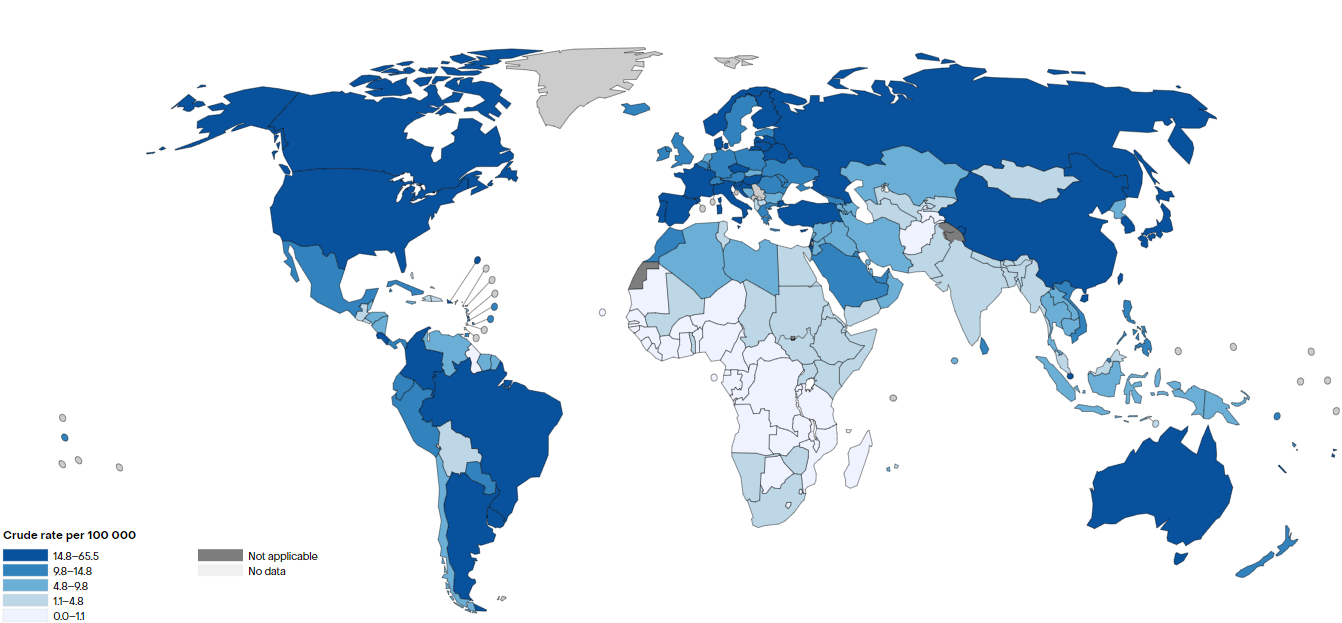
\includegraphics[width=1.00 \textwidth]{1/figures/tb_inc_ct_mujeres.png}
		\caption[Tasa bruta de incidencia de cáncer de tiroides en mujeres por 100 000 personas]{Tasa bruta de incidencia de cáncer de tiroides en mujeres por 100 000 personas. \\
		Fuente: \cite{ws_oms2022cancert}. \textit{Cancer Today}.}
		\label{1:fig}
	\end{center}
\end{figure}


\begin{figure}[H]
	\begin{center}
		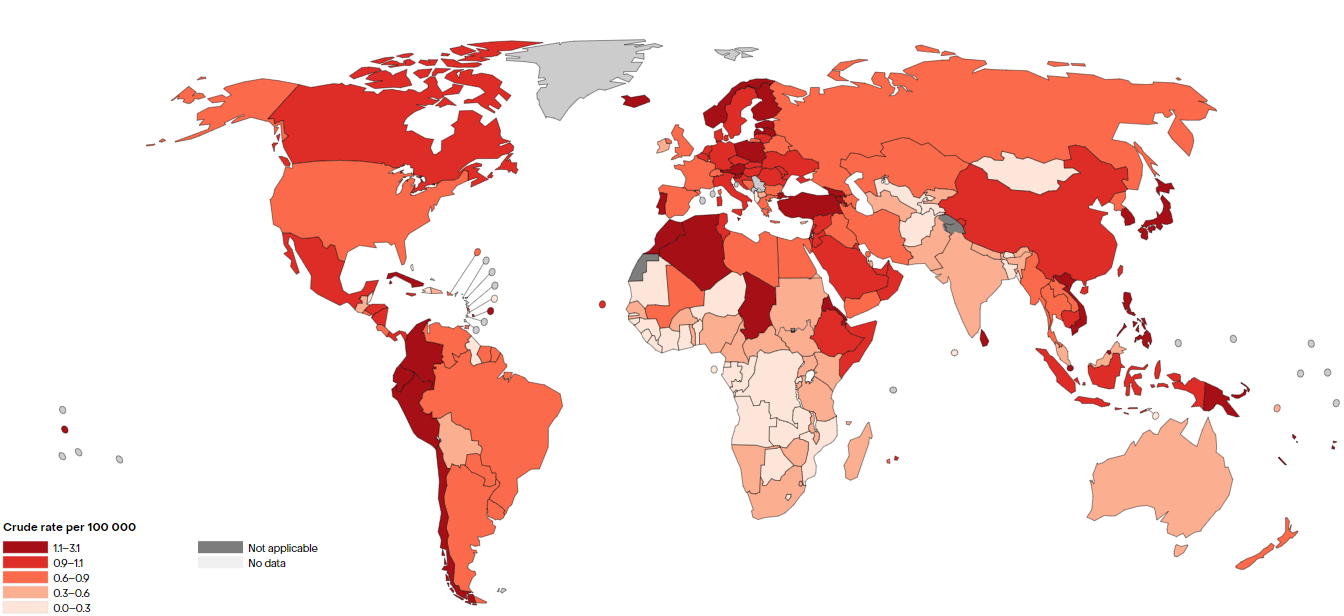
\includegraphics[width=1.00 \textwidth]{1/figures/tb_mor_ct_mujeres.png}
		\caption[Tasa bruta de mortalidad de cáncer de tiroides en mujeres por 100 000 personas]{Tasa bruta de mortalidad de cáncer de tiroides en mujeres por 100 000 personas. \\
		Fuente: \cite{ws_oms2022cancert}. \textit{Cancer Today}.}
		\label{1:fig2}
	\end{center}
\end{figure}

De igual forma, en el caso de los varones, el Perú también se encuentra entre los rangos más altos de incidencia y mortalidad. A continuación, se muestran sus respectivas gráficas.

\begin{figure}[H]
	\begin{center}
		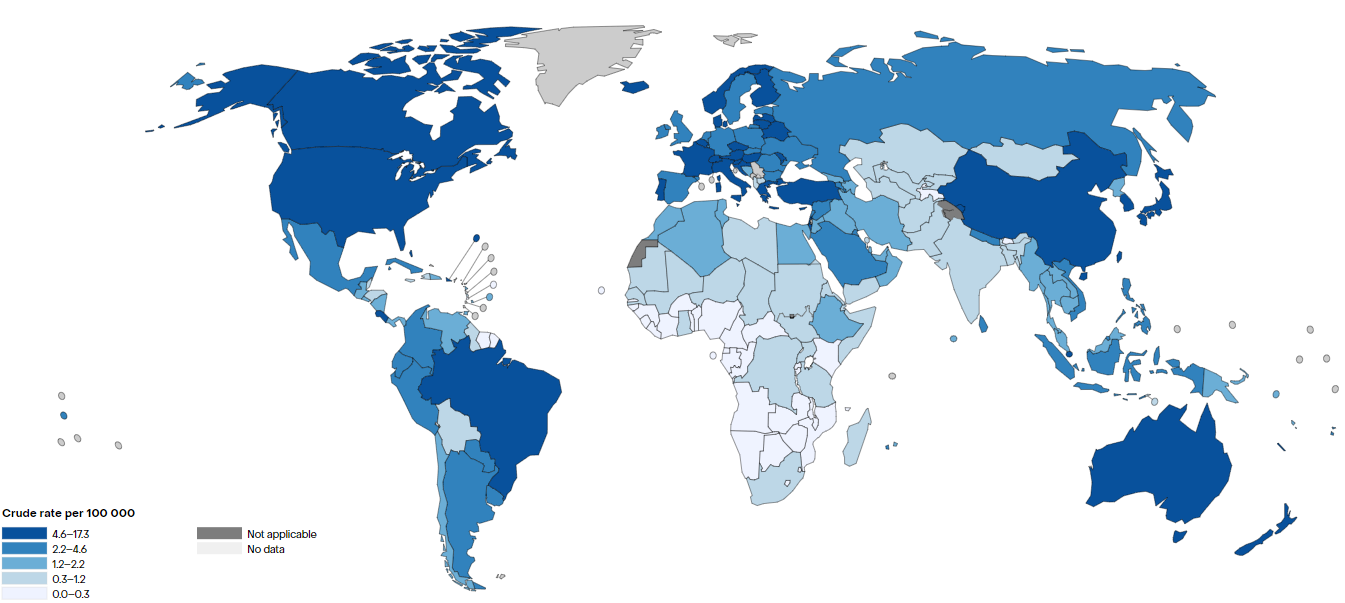
\includegraphics[width=1.00 \textwidth]{1/figures/tb_inc_ct_varones.png}
		\caption[Tasa bruta de incidencia de cáncer de tiroides en varones por 100 000 personas]{Tasa bruta de incidencia de cáncer de tiroides en varones por 100 000 personas. \\
		Fuente: \cite{ws_oms2022cancert}. \textit{Cancer Today}.}
		\label{1:fig3}
	\end{center}
\end{figure}

\begin{figure}[H]
	\begin{center}
		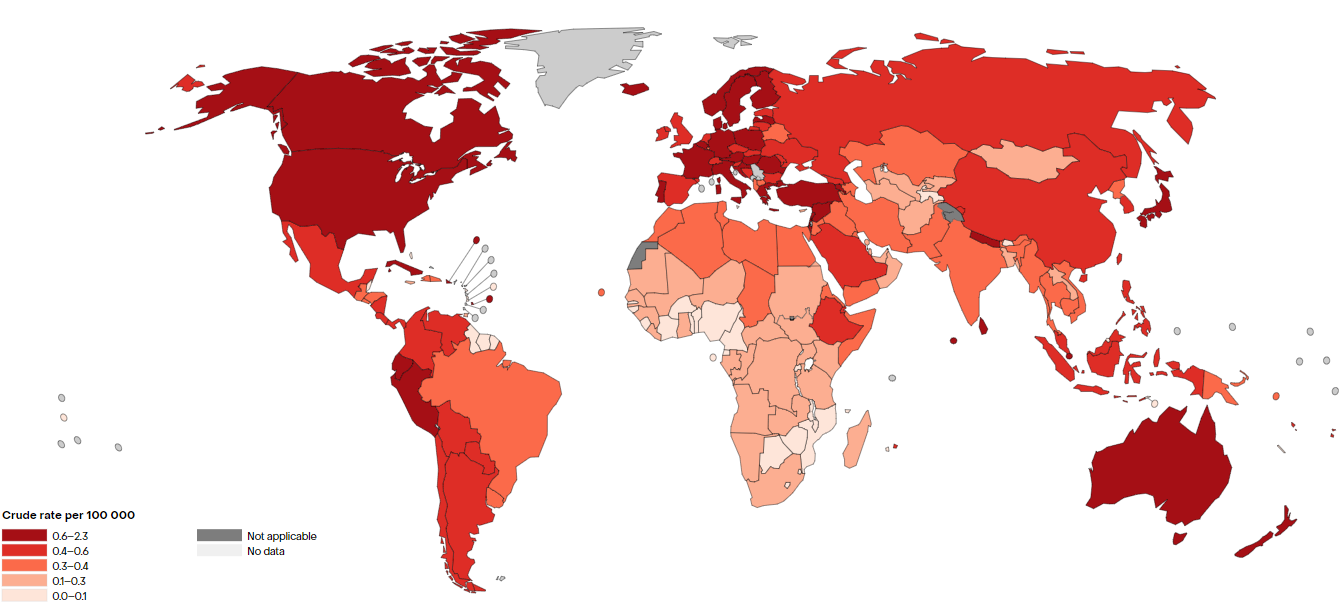
\includegraphics[width=1.00 \textwidth]{1/figures/tb_mor_ct_varones.png}
		\caption[Tasa bruta de mortalidad de cáncer de tiroides en varones por 100 000 personas]{Tasa bruta de mortalidad de cáncer de tiroides en varones por 100 000 personas. \\
		Fuente: \cite{ws_oms2022cancert}. \textit{Cancer Today}.}
		\label{1:fig4}
	\end{center}
\end{figure}

Con el siguiente gráfico que muestra los mismos índices distribuidos por género y regiones del mundo, es fácil notar la alta incidencia de este tipo de cáncer en las mujeres, siendo la región con mayor incidencia América del Norte, mientras que la de mayor mortalidad es Oceanía. La región de Latino América y el Caribe supera a Norte América en mortalidad, aunque se encuentra por debajo de Oceanía y Europa.

\begin{figure}[H]
	\begin{center}
		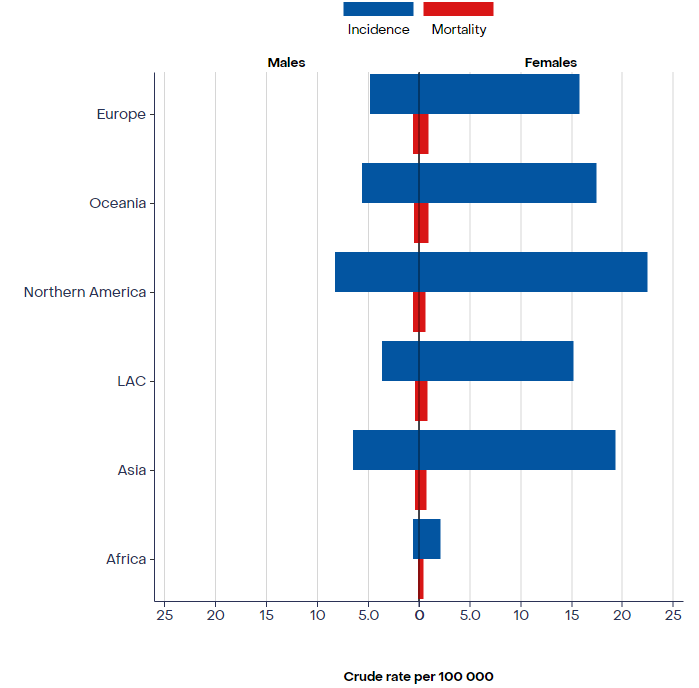
\includegraphics[width=0.60 \textwidth]{1/figures/tb_inc_mor_gen_y_reg.png}
		\caption[Tasa bruta de incidencia y mortalidad de cáncer de tiroides por género y región]{Tasa bruta de incidencia y mortalidad de cáncer de tiroides por género y región. \\
		Fuente: \cite{ws_oms2022cancert}. \textit{Cancer Today}.}
		\label{1:fig5}
	\end{center}
\end{figure}

Además, es importante mencionar que este aumento de incidencia a nivel global de cáncer de tiroides se debe a diversos factores relacionados a problemas de salud como la obesidad y a factores medioambientales como por ejemplo exposición al yodo \parencite{pr_kim2020geoinflu}. Sin embargo, otro factor es la poca disposición y capacidad de realizar un diagnóstico a tiempo de los nódulos tiroideos que, de forma general, cerca del 7\% al 15\% de los casos de llegan a ser cancerígenos \parencite{pr_haugen2016amethy}.

Para la detección temprana de este tipo de cáncer o desarrollo de tumores, depende en gran medida de la experiencia y la capacidad cognitiva de un experto en radiología, y muchos de estos se ven en la necesidad de utilizar no muy avanzados sistemas de diagnóstico por computadora, mejor conocido como CAD por sus siglas en inglés \parencite{pr_zhu2021agendlframew}. Ante grandes limitaciones de sistemas CAD básicos, y aprovechando el extenso uso de la inteligencia artificial, el Deep Learning y sus algoritmos son capaces de incorporar mayor eficacia a dichos sistemas.

El Deep Learning ha sido usado ampliamente como herramienta para el procesamiento de imágenes médicas, no solo para detectar diferentes tipos de cáncer o nódulos como los relacionados a los pulmones, sino también para la retinopatía diabética y localización de feto en ecografías, e inclusive en la detección del COVID-19 \parencite{pr_bhatta2021medimage}. Además, el aumento de la calidad de imágenes de ultrasonido que se fue desarrollando en los últimos 30 años, aumentando cada vez más resolución de las imágenes y el tiempo de adquisición, ha permitido una mejora en términos de detección de enfermedad; sin embargo, aún se requiere de un médico especializado y debidamente entrenado para lograr un realizar un correcto análisis de las imágenes, por ello se vio en la necesidad de encontrar métodos de clasificación automatizada, pero dichos métodos antiguos consumían bastante tiempo, gran poder computacional y poca capacidad de generalización de resultados, es así que en este contexto, apareció una novedosa arquitectura de Deep Learning que actualmente es usado en diferentes área el día de hoy: las Redes Neuronales Convolucionales o CNN, quitando en gran medida los problemas de las antigua técnicas \parencite{pr_signgh20203ddl}. Aunque existe varios antecedentes con esta técnica de Deep Learning en detección de nódulos en la tiroides, muy pocos se han centrado en el grado de ayuda que se brinda a un médico especialista, ya que una simple detección no aceleraría debidamente el proceso de descarte de una anomalía en la tiroides.


\section{Formulación del Problema}
Con el objetivo de formular los objetivos de esta investigación, se propusieron las siguientes preguntas.
\subsection{Problema General}
PG: \newcommand{\ProblemaGeneral}{
¿Es posible implementar un modelo de Deep Learning para el diagnóstico de nódulos tiroideos a través de imágenes de ultrasonido?
}
\ProblemaGeneral
\subsection{Problemas Específicos}
\newcommand{\Pbone}{
¿Qué características del conjunto de datos a usar para entrenar y evaluar los modelos son ideales para obtener buenos resultados?
}
\newcommand{\Pbtwo}{
¿Qué técnicas de preprocesamiento se deberían aplicar a las imágenes de ultrasonido del conjunto de datos?
}
\newcommand{\Pbthree}{
¿De qué forma se puede evaluar el rendimiento de los modelos de Deep Learning en la clasificación de imágenes de ultrasonido?
}
\newcommand{\Pbfour}{
¿Qué arquitecturas de Deep Learning tienen el más alto desempeño en la clasificación de imágenes de ultrasonido de la tiroides?
}

\begin{itemize}
	\item PE1: {\Pbone}
	\item PE2: {\Pbtwo}
	\item PE3: {\Pbthree}
	\item PE4: {\Pbfour}
\end{itemize}

\section{Objetivos de la Investigación}
A continuación, se presentan el objetivo general y los objetivos específicos.
\subsection{Objetivo General}
OG: \newcommand{\ObjetivoGeneral}{
Diseñar un modelo de Deep Learning para el de diagnóstico de nódulos tiroideos a través de imágenes de ultrasonido.
}
\ObjetivoGeneral
\subsection{Objetivos Específicos}
\newcommand{\Objone}{
Determinar las características ideales del conjunto de datos a usar para entrenar y evaluar los modelos.
}
\newcommand{\Objtwo}{
Determinar las técnicas de preprocesamiento que se deben aplicar a las imágenes de ultrasonido del conjunto de datos.
}
\newcommand{\Objthree}{
Identificar las métricas de evaluación de rendimiento de los modelos de Deep Learning en la clasificación de imágenes de ultrasonido.
}
\newcommand{\Objfour}{
Determinar las arquitecturas de Deep Learning que tienen el más alto desempeño en la clasificación de imágenes de ultrasondio de la tiroides.
}

\begin{itemize}
	\item OE1: {\Objone}
	\item OE2: {\Objtwo}
	\item OE3: {\Objthree}
	\item OE4: {\Objfour}
\end{itemize}



\section{Justificación de la Investigación}

\subsection{Teórica}
La investigación se desarrolla con el propósito de otorgar mayor conocimiento sobre el uso de la inteligencia artificial en el diagnóstico de nódulos en la glándula de la tiroides, esto a través de imágenes de ultrasonido. Esta investigación aportará conocimiento sobre el diseño y eficacia de los sistemas de diagnóstico asistido por computadora con base en el Deep Learning en el diagnóstico de nódulos tiroideos. Esto servirá para que en un futuro se generen nuevos y más eficaces sistemas de apoyo médicos dentro de esta área.

\subsection{Práctica}
Los antecedentes presentados en la investigación califican la capacidad de un modelo de Deep Learning en la detección y diagnóstico de una imagen de ultrasonido de la tiroides, esto usando diferentes algoritmos y técnicas con el objetivo de aumentar la capacidad el modelo. Muchos de estos abarcan la parte de clasificar una imagen, mientras que otros realizan segmentación del área donde el nódulo se está desarrollando, basándose además en estándares médicos de diagnóstico. Muy pocos realizan ambos: clasificación y segmentación. La presente investigación se centrará en desarrollar un modelo de clasificación. 

\subsection{Metodológica}
El modelo desarrollado en la investigación no propone un reemplazo de los médicos especialistas en el área, sino una herramienta potente para estos que ayudará a diagnosticar los nódulos que se desarrollan en la glándula de tiroides. La investigación presentará y concluirá con las herramientas tecnológicas y técnicas de Deep Learning ideales para el desarrollo de sistemas de diagnóstico asistido por computadora, esto luego de una extensa recopilación de datos y métodos que permitan la construcción y desarrollo de un modelo eficiente y eficaz.

\section{Delimitación del Estudio}
A continuación, se presentará la delimitación espacial, temporal y conceptual.

\subsection{Espacial}
Debido a que la problemática y necesidad de diagnosticar a tiempo los nódulos tiroideos no es propio de una región o país, la mayoría de la data para realizar un correcto análisis de inteligencia artificial son basados en países extranjeros y de gran alcance como Estados Unidos, India y China. Los proyectos previos más afines al tema presentados en la investigación son desarrollados en diversos países extranjeros. 

\subsection{Temporal}
Los datos presentados en esta investigación sobre casos de incidencia y mortalidad de la tiroides son hasta el 2022. De igual forma, las imágenes de ultrasonido de glándulas de tiroides con presencia de nódulos que se usarán para entrenar y validar el modelo de clasificación son recopiladas del conjunto de datos de acceso libre TNCD recolectada hasta finales del año 2022. Los antecedentes relacionados a esta investigación fueron publicados entre el 2019 y 2023.

\subsection{Conceptual}
La presente investigación se centrará en el desarrollo de un modelo de Deep Learning para realizar la clasificación de nódulos de la glándula de tiroides y así lograr determinar si es de carácter benigno o maligno. 

%\chapter{Marco Teórico}
\section{Antecedentes de la investigación}
En esta parte de la investigación se presentan algunos antecedentes relacionados a la detección y diagnóstico de nódulos en distintos órganos y a través de diversas metodologías. Estos ayudarán a entender el enfoque y obtener bases para un correcto desarrollo del proyecto en cuestión.

\cite{pr_moreira2021deteclung} presenta una investigación relacionada a la elaboración de un sistema CAD (Computer-aided Detection) para la detección y segmentación de nódulos presentes en los pulmones.

Para realizar esta investigación, se tuvo en consideración la realidad que se atraviesa a nivel mundial sobre el cáncer de pulmón, y como este afecta a las personas sin importan su género, convirtiéndolo uno de los tipos de cáncer más mortales según la investigación mencionada. 

La presencia de nuevas formas de detectarlo como el uso de tomografías computarizadas tuvo un gran impacto para la detección temprana de los nódulos en estos órganos, ya que estos pueden significar un futuro desarrollo de cáncer. Sin embargo, realizar un análisis de este tipo de imágenes médicos no era nada trivial debido al complejo proceso de análisis con estas tecnologías. Ante esto, el Deep Learning apareció con una herramienta eficaz para ayudar a los médicos en el análisis de estas imágenes; sin embargo, pese a sus grandes ventajas, su aplicabilidad es muy limitada. Por tal motivo, esta tesis incluye modernos enfoques y técnicas para una detección automática de nódulos pulmonares.

De forma general, el algoritmo presentado en esta investigación consiste en dos bloques. El primero de estos se encarga de la detección de nódulo a través de técnicas de detección de objetos, mientras que el segundo se encarga de la segmentación de este. Los resultados obtenidos fueron del 79\% en recall; sin embargo, esto no fue suficiente para poder considerar al modelo como robusto, por ello, posteriormente, se utilizaron técnicas innovadoras en colaboración expertos en el área. Las anotaciones de los especialistas, junto con los resultados del sistema, mejoraron el desempeño general de la detección.

Para aumentar aún más las capacidades del sistema, se desarrolló en la parte final de la investigación un modelo de Deep Learning para la detección automática y la segmentación de nódulos pulmonares a través de imágenes tomográficas. Este también consistió en dos bloques, uno encargado de la segmentación automática y otro que corrige el anterior en base a dos puntos en los límites del nódulo. El modelo consiguió demostrar su capacidad para corregir la segmentación de nódulos pequeños, además de segmentar los nódulos no sólidos, los cuales presentaban un reto para el sistema.

\cite{pr_felgueiras20193dlungnod} reafirman la importancia de construir este tipo de sistemas mencionando al cáncer de pulmón como el principal tipo de cáncer en causar muertes en todo el mundo.

El sistema desarrollado en esta investigación fue basado también en el diagnóstico a través de imágenes tomográficas que comúnmente es realizado por un médico experto; sin embargo, se menciona que este análisis siempre está sujeto a errores ya que existe mucha subjetividad en este tipo de diagnóstico, lo que conlleva muchas veces errores de detección. Además de la existencia de la tendencia al rechazo hacia esto tipo de sistemas CADx (Computer-aided Diagnosis) por parte de los médicos, esto debido a la fata de comprensión del cómo se realiza este tipo de diagnóstico.

Para afrontar esta desconfianza a este tipo de sistemas, se menciona la existencia del Deep hierarchical semantic convolutional neural network (HSCNN) que añadía a la capacidad de predecir si un nódulo era maligno o benigno, la función de otorgar evidencia visual del diagnóstico a través de la predicción de las características del nódulo. Sin embargo, el conjunto de datos usado en esta investigación difería de las evaluaciones de los propios médicos. Por tal motivo, en la presente investigación se puso como un objetivo probar si la disminución de esta varianza en los datos podría mejorar los resultados del modelo HSCNN.

A través de un análisis de los datos, se logró mejorar la descripción de características. Este nuevo conjunto de datos fue revisado por especialista para comprobar su validez antes de ser ingresado al modelo HSCNN para predecir si un nódulo era maligno o benigno. Este proceso se hizo a través de un k-folds igual a 4 junto con cross-validation.

Los resultados fueron comparados con el modelo inicial, y se obtuvo que el nuevo HSCNN era mejor solo cuando se trataba de predecir si un nódulo era maligno. Las métricas del nuevo modelo fueron de 0.78 en accuracy, el AUC de la curva ROC es de 0.74, una sensibilidad 0.83 y una especificidad de 0.89, frente a las métricas de modelo original que obtuvo un accuracy de 0.84, un AUC de la curva ROC de 0.86, sensibilidad de 0.71 y una especificidad de 0.89. Esto significó que el modelo se equivocaba más cuando los nódulos a analizar eran pequeños. En general, los resultados distaron de los propios del modelo inicial, esto es debido a la reducción considerable de imágenes del conjunto de datos original. 

\cite{pr_supanta2021desalgdetec} menciona la incidencia de cáncer de pulmón en el Perú en el periodo 2010-2012 con un gran número de 3 121 casos diagnosticados, convirtiéndolo en el tercer tipo de cáncer más común en el país, y ocupa el segundo lugar en mortalidad con un número de 2 591 de muertes en el mismo periodo, esto debido al tardío diagnóstico de este mal. Por este motivo, es obvia la necesidad de realizar un examen de detección temprana donde es posible un tratamiento y, posteriormente, una posible cura a esta enfermedad. 

La investigación presenta una forma de realizar detección de nódulos pulmonares a través de imágenes radiográficas digitales que comúnmente presentan problemas como baja claridad y resaltado de las características, por ende, generan dificultades para realizar un correcto análisis de este tipo de imágenes. Las técnicas usadas son corrección gamma, análisis de proyecciones, erosión, filtros geométricos, dilatación, filtro de convergencia y la umbralización por el método Otsu, esto aplicado a un conjunto de datos de 50 radiografías de tórax.

Los resultamos muestran una sensibilidad del 0.91, especificidad de 0.96 y precisión de 0.94. 

Otra investigación relacionada a detectar alguna enfermedad a través de técnicas de Deep Learning y visión por computadora es la presentada por \cite{pr_monroy2021disvc} donde toma a la enfermedad de Parkinson como mal a detectar, y esto a través del análisis de la escritura de una persona. Para tal objetivo, en la investigación se desarrolló un modelo de visión computacional para el prediagnóstico de esta enfermedad.

La metodología empieza con la adquisición y preprocesamiento de los datos, para posteriormente usar técnicas de extracción de características como SIFT, SURF, ORB y HOG. Estos serán ingresados a un modelo de Machine Learning (SVM, RF, KNN) que finalmente realizará una clasificación. Además, se usaron diferente arquitectura de redes neuronales convolucionales como Inception, VGG16, VGG19, LeNet y ResNet50.

Los resultados finales fueron un 0.99 en accuracy, 0.99 en precisión, 0.99 en recall, 0.98 en F1-score y AUC.

\cite{pr_kang2022thysegclass} muestran la frecuencia de diagnóstico de nódulos tiroideos, esto en el rango de 19\% y 68\% de casos clínicos. El cáncer de tiroides es el número 9 en incidencia, mientras que es el número 6 en mortalidad, esto a nivel mundial según datos del 2018.

Se menciona que es importante tener métodos menos invasivos para determinar el cáncer de tiroides, teniendo en cuenta además que es necesario la detección a tiempo, pues esto aumenta la probabilidad de ser curado. El análisis de imágenes de ultrasonido es una buena opción a el análisis de, por ejemplo, cirugías. Sin embargo, este diagnóstico depende mucho de la experiencia del médico especialista, lo cual vuelve a este tipo de análisis muy subjetivo.

La segmentación y clasificación son herramientas claves dentro de un sistema de diagnóstico asistido, siendo ambos muy relacionados entre sí, pues comparten ciertas características de las imágenes (bordes de las imágenes pueden ser usados para la clasificación y segmentación). Afrontar ambas tareas al mismo tiempo en un solo modelo podría ser más robusto.

La red MTL propuesta en uno de los antecedentes es similar a una red de segmentación multiclases que genera como salida mapa de segmentación y predicciones categóricas.

La investigación presentada en este antecedente se centra también en una red MTL que también realizará procesos de segmentación y clasificación.

La metodología empieza con la data. Esta fue recolectada del West China Hospital. Se tuvieron 4 493 imágenes de ultrasonido, cada uno de un paciente. En específico, 2 576 imágenes pertenecen a nódulos benignos, mientras que 1 917 son malignos. Las anotaciones fueron verificadas por especialistas.

Para la evaluación de la clasificación se usó el accuracy, f1-score, ROC, área bajo la curva ROC (AUC). En el caso de la segmentación, se usó Dice coefficient y Intersection of Union (IoU).

Además, se definieron 3 medidas para cuantificar la inconsistencia al nivel de las tareas. El primero de estos evalúa a la clasificación, el segundo por la tarea de segmentación de segunda clase, y el tercero es para la segmentación de tercera clase.

El modelo construido en esta investigación se basó en MSL (Multi Stage Learning) y MTL (Multi Task Learning). Se diseño una red MS-MTL. Además, se determinó diferentes tipos de consistencia de tareas: intra e inter task consistency.

Los resultados fueron extraídos de 3 modelos CIsNet, MS-MTL y MS-MTL con intra e inter task consistency. La medida AUC obtenida para cada modelo es 0.9277, 0.9523 y 0.9608, respectivamente. Además, se determinó que el intra task cosistency y el MSL aumenta el desempeño de la segmentación. El caso de inter task consistency con MTL mejora el desempeño de las tareas de clasificación y segmentación. Con la combinación de ambas tareas de consistencias también se demuestra su efectividad.

El método usado en esta investigación se muestra a continuación.

\begin{figure}[H]
	\begin{center}
		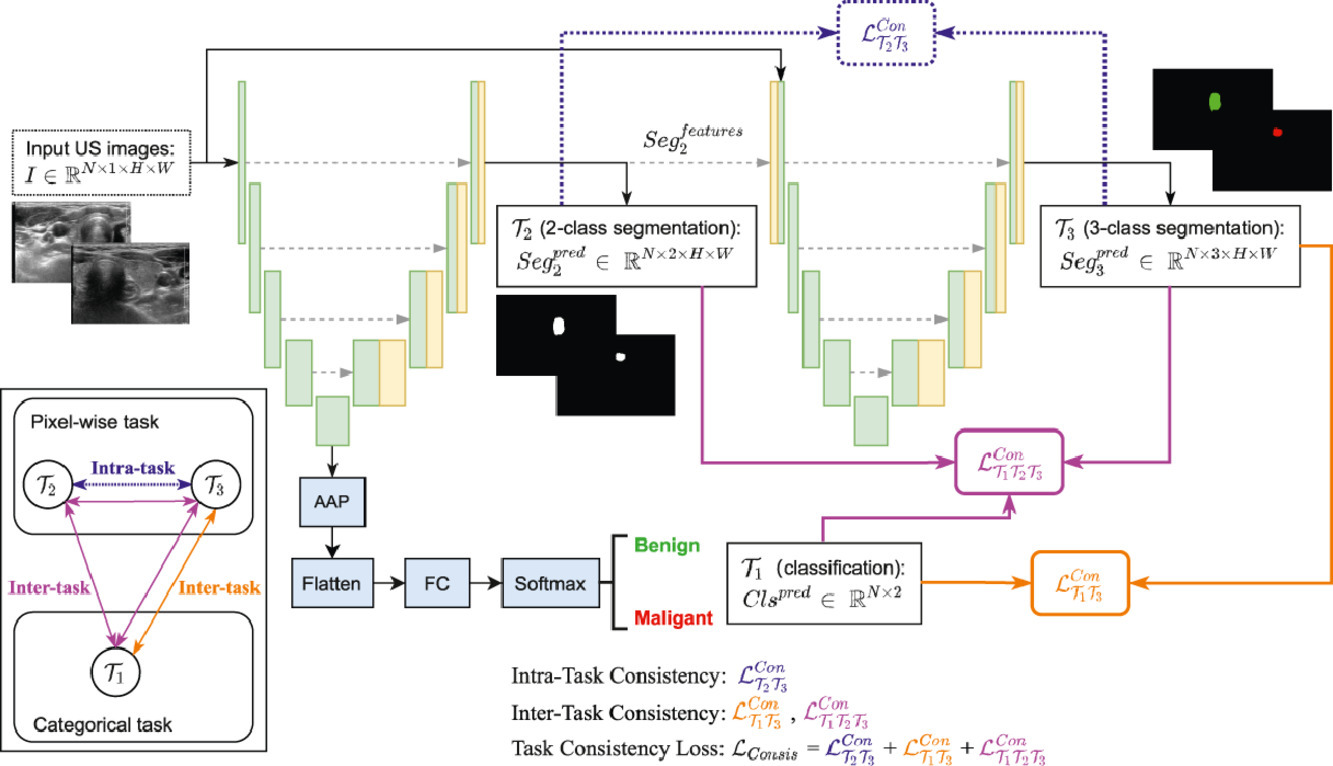
\includegraphics[width=1.00\textwidth]{2/figures/antecedente_4.jpg}
		\caption[Representación del método desarrollado]{Representación del método desarrollado. \\
		Fuente: \cite{pr_kang2022thysegclass}. \textit{Thyroid nodule segmentation and classification in ultrasound images through intra- and inter-task consistent learning}.}
		\label{2:fig101}
	\end{center}
\end{figure}


\cite{pr_sun2023classthynvit} presenta el problema de diagnosticar nódulos tiroideos nivel 3 debido a pocas características representativas que diferencien a los nódulos benignos de nivel 3 con los nódulos malignos, esto conlleva a obtener bajas precisiones en el diagnóstico. Ante esto, en el artículo se presenta un modelo clasificador de nódulos tiroideos con ViT (Vision-Transformer-based) y el contrast learning. Estas técnicas ayudaron a minimizar la distancia de características en nódulos de una misma clase, lo cual mejora la capacidad predictiva del modelo. Finalmente, en la fase de testeo del modelo se logró un accuracy de 0.869, mientras que las demás métricas indican la superioridad frente a otros modelos clásicos de Deep Learning que también son usados para clasificar.

En la siguien figura se presenta la arquitectura de Vison Transformer desarrollada.

\begin{figure}[H]
	\begin{center}
		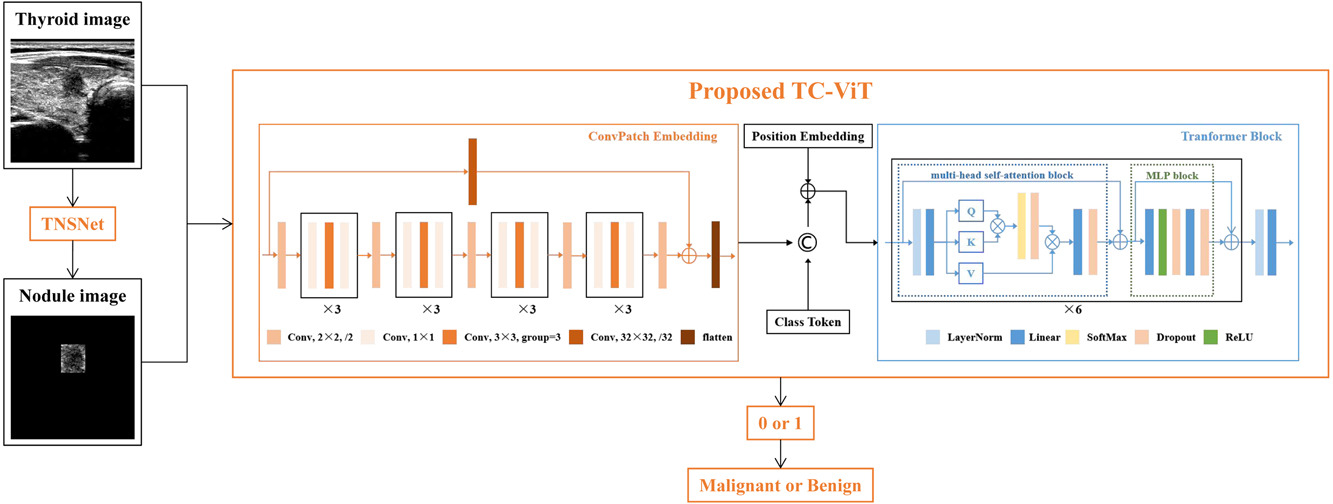
\includegraphics[width=1.00\textwidth]{2/figures/antecedente_5.jpg}
		\caption[Arquitectura de modelo TC-ViT]{Arquitectura de modelo TC-ViT. \\
		Fuente: \cite{pr_sun2023classthynvit}. \textit{Classification for thyroid nodule using ViT with contrastive learning in ultrasound images}.}
		\label{2:fig102}
	\end{center}
\end{figure}


\cite{pr_zhang2023madlap} presenta el nivel de importancia de poseer una buena base de datos etiquetada correctamente para lograr entrenar un buen modelo de Machine Learning. En este artículo se desarrolla y presenta a la herramienta Multistep Automated Data Labelling Procedure (MADLaP) que facilita y automatiza el proceso de etiquetado de datos relacionados a nódulos tiroideos. Este incluye el procesamiento de leguaje natural basado en reglas, el Deep Learning para segmentación de imágenes y el reconocimiento óptico de caracteres. MADLaP fue desarrollado en la fase de entrenamiento con datos de 378 pacientes, mientras que en la fase de prueba se usaron datos de 93. Este obtuvo finalmente un accuracy de 0.83.

\cite{pr_deng2022autclass} ponen al cáncer de tiroides como el que más ha prevalecido en las últimas 3 décadas. Existen diversos sistemas que ayudan a la detección de los nódulos en esta glándula; sin embargo, muchos de estos solo se limitan a determinar si un nódulo es maligno o benigno, y no muestran el porqué de la toma de esa decisión por parte del sistema, lo cual genera desconfianza entre los especialistas al momento de usarlos. Para afrontar esto, se desarrolla primeramente una estratificación de riesgo basada en el léxico estandarizado ACR TI-RADS. Posteriormente, se realiza la clasificación entre benigno y maligno. De formar general, el método realizará una caracterización del nódulo basado en ACR TI-RADS para detectar su nivel de riesgo y la clase al que pertenece (benigno o maligno). Los resultados muestran en la evaluación un accuracy de 0.9355, un sensitivity de 0.9386 y una specificity de 0.9314. 

Se realizó la notación de las imágenes de nódulos con los indicadores del diccionario de ACR TI-RADS. Para afrontar el desbalanceo de la data, se realizó un proceso de mejora de la data creando imágenes a través de giros, recortes y mezclas. Se extrajeron las áreas de interés de las imágenes a través de una red en cascada. Se quitaron las anotaciones manuales en las imágenes (limpieza de imagen). Una vez concluido con el procesamiento de las imágenes, se realizó la construcción y ejecución del modelo de Deep Learning Multi-Task Learning (MLT). Finalmente, el modelo obtenido fue comparado con otros a través de los siguientes indicadores: accuracy, sensitivity, specificity y el área bajo la curva. 

\cite{pr_wang2020autodiag} mencionan que los nódulos tiroideos son uno de los primeros síntomas que podrían conllevar a un cáncer en la tiroides. Este tipo de cáncer es uno de los que tiene mayor incidencia y que esta tendencia ha ido en crecimiento durando los últimos 30 años.

Además, se menciona que, para ayudar a esta detección, se han propuesto anteriormente varios sistemas de diagnóstico asistido; sin embargo, estos solo realizan dicho proceso a través de solo una imagen de ultrasonido en vez de usar todas aquellas que se obtienen de un examen. Por esto, en este artículo, se desarrolla un modelo de Deep Learning para el diagnóstico de tiroides a través de varias imágenes de ultrasonido. Esto a través de una integración de todas las características de las imágenes realizadas en un examen. 

La base de datos usada fue construida, y se obtuvieron resultados perfectamente comparables con los resultados de los antecedentes revisados en este artículo.

La metodología consistía en la construcción de tres redes distintas: feature extraction network, attenntion-based feature aggregation network, classification network. Estas tres redes juntas forman el modelo objetivo desarrollado en este artículo.

En general, la metodología consistía en, primero, la construcción del conjunto de datos que se conforma de imágenes de ultrasonido procedentes de un hospital. Se recolectaron cerca de 7 800 imágenes de 1 046 exámenes de entre los años 2015 y 2018. En segundos lugar, se realizó el etiquetado de los datos. Estas anotaciones se realizaron de acuerdo con los exámenes en general, y no a cada una de las imágenes que la conforman. Luego, se realizó la separación de la data en entrenamiento, prueba y validación. En la parte final de experimentación, se realizó un preprocesamiento con data augmentation y se definió 100 épocas para la fase de entrenamiento. El modelo ganador de la fase de validación fue probado con la data de prueba. Las métricas usadas para la evaluación fueron el accuracy, sensitivity (true positive rate) y el área bajo la curva (AUC ROC).

La siguiente figura muestra la arquitectura propuesta en esta investigación.

\begin{figure}[H]
	\begin{center}
		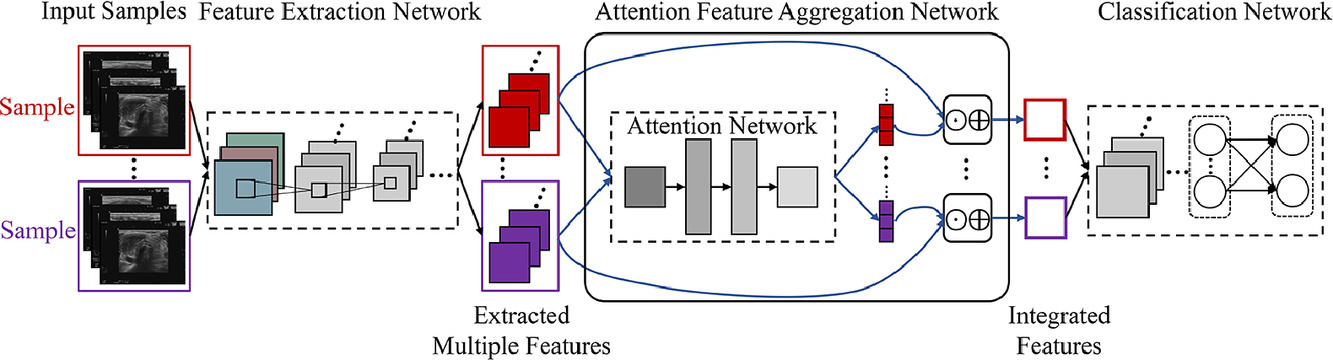
\includegraphics[width=1.00\textwidth]{2/figures/antecedente_8.jpg}
		\caption[Arquitecura de la red desarrollada]{Arquitecura de la red desarrollada. \\
		Fuente: \cite{pr_sun2023classthynvit}. \textit{Automatic diagnosis for thyroid nodules in ultrasound images by deep neural networks}.}
		\label{2:fig103}
	\end{center}
\end{figure}


\cite{pr_sun2022tnsnet} mencionan que, en el sistema endocrino, un problema muy común son los nódulos tiroideos. Normalmente estos pueden ser sólidos o de otras variadas texturas. La incidencia de esta enfermedad se ha ido incrementando a través de los años. Comúnmente se usan las imágenes de ultrasonido para detectar estos nódulos, esto lo hacen en tiempo real, tiene bajo costo y no es invasivo, por cual es una buena opción. Estas imágenes pueden otorgar información valiosa de los nódulos como los márgenes, ecogenicidad, calcificación, composición, etc. Además, existe el Thyroid Image Reporting y el sistema de datos TI-RADS pueden cuantificar las características otorgadas por las imágenes de ultrasonido y evaluar si es benigno o maligno. Sin embargo, estas imágenes pueden traer problemas como bajo contraste y ruido de moteado, lo cual genera retos para extraer sus características. Este problema puede superarse a través de una correcta segmentación de los nódulos tiroideos. Así, la segmentación es un paso importante para realizar diagnóstico correcto. Esto puede ser aplicado a la evaluación automática en TI-RADS para facilitar la clasificación de los nódulos. Se añadió un shape-supervised path para mejorar la identificación de la forma, y así lograr una mejor segmentación.

La data que usaron se obtuvo de diversos escáneres disponibles comercialmente, juntando 3 786 imágenes de ultrasonido de nódulos tiroideos. Posteriormente, se realiza un preprocesamiento para estandarizar la data. Se realizó un proceso de limpieza de las imágenes para quitar los datos privados de los pacientes, y borrar imágenes erróneas. Se propuso TNSNet para asegurar una mejor detección y segmentación. Este modelo es un dual-path network que contiene dos partes region path y shape path. Ambos caminos se enfocan en las características de bordes y texturas (cada uno de estos para cada camino).

Se diseñó un dual-path loss function para el entramiento de ambos caminos del modelo. Para el camino de región, se usó el binary cross-entropy loss y el generalized Dice loss, ambos para entrenar la región de segmentación de los nódulos tiroideos. En el caso del segundo camino (camino de la forma) se combinó el Hausdoff distance loss y un modificado active contour loss. Esto fue construido para el entrenamiento del contorno de segmentación.

Las métricas usadas para evaluar la segmentación del modelo son Dice simialrity coefficient (DSC), sensitivity, specificity y el accuracy.

Los resultados muestran que en el caso de los nódulos benignos todos los modelos (el construido en el artículo y los de referencia) logran buenos resultados, esto debido a la buena calidad de las imágenes. En el caso de los nódulos malignos, el modelo TNSNet superó por completo a los otros modelos de referencia. Hubo otros experimentos, en los cuales, el modelo presentado en este artículo, de manera general, obtuvo mejores resultados.

La investigación realizada por \cite{pr_yang2023novelViTscc} se centra en la problemática del cáncer de piel, específicamente en el grave problema de los melanomas y la alta necesidad de una detección temprana para mejorar las posibilidades de supervivencia de los pacientes con este mal.

Además, se menciona que aunque la técnica más usada para la detección de melanomas es la dermatoscopia, su precisión es muy variada dependiendo el tipo de cáncer de piel con el que se está tratando. En este contexto, las técnicas de Deep Learning han demostrado ser un herramienta capaz de mejorar la precisión en las tareas relacionadas a clasificar el cáncer de piel, incluso superando al desempeño de los propios dermatólogos.

A pesar de estos logros del desarrollo de Deep Learning en esta área, se menciona que aún hay dificultad para la clasificación de algunos tipos de cáncer de piel como el melanoma. Por este motivo se propone una nueva arquitectura de red basada en los transformadores con el objetivo de mejorar la capacidad de los algoritmos de clasificación de cáncer de piel.

La metodología seguida por los autores inicia con la preparación de los datos. En este caso se usó el conjunto de datos HAM10000 que consta de 7 clases distintas de cáncer de piel. Las imágenes tuvieron que ser redimensionadas para los 4 distintos modelos a entrenar: Inception ResNet con Soft Attention (IRv2 + SA), ResNet50 con Soft Attention (ResNet50 + SA), ViTfSCD-Large y ViTfSCD-Base. Los parámetros de estos dos últimos modelos se muestran en la siguiente figura.

Además, se aplicó a las imágenes una limpieza, eliminando los duplicados. También pasó por un proceso de balanceo de las clases donde se intentó igualar la cantidad de imágenes en cada una de estas. Se realizó el proceso de aumento de datos a través de modificaciones en las imágenes como alterar la saturación de forma aleatoria, cambiar el contraste y el brillo. Finalmente, se definió los porcentajes de división para el conjunto de datos, siendo 85\% para el entrenamiento y 15\% para la prueba. 

Para la evaluación de los modelos se utilizaron las métricas de accuracy, precision, recall (sensitivity), specificity y F1 score. Los resultados de evaluar su capacidad de clasificación de los 4 modelos se muestran a continuación.

\begin{figure}[H]
	\begin{center}
		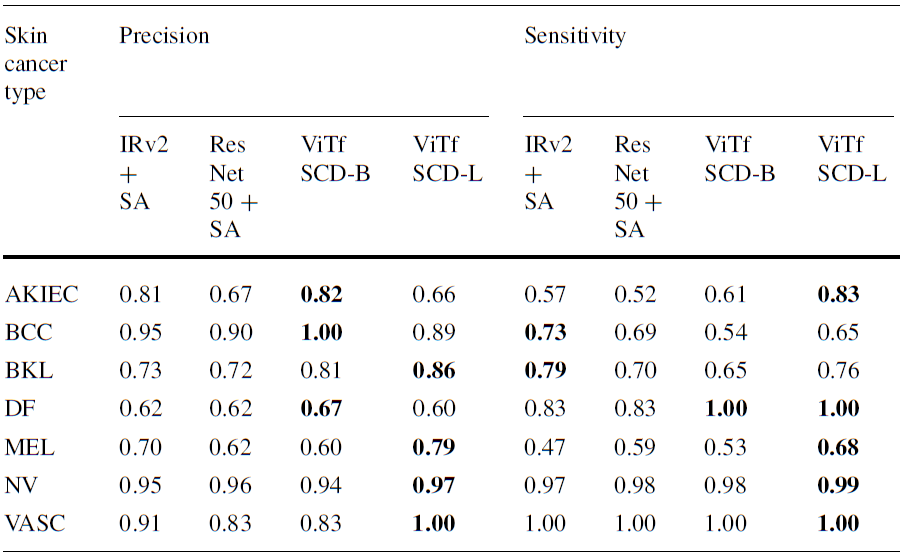
\includegraphics[width=1.00\textwidth]{2/figures/vitpaper1_part1.png}
		\caption[Comparación de resultados de los modelos (precision y sensitivity)]{Comparación de resultados de los modelos (precision y sensitivity). \\
		Fuente: \cite{pr_yang2023novelViTscc}. \textit{A Novel Vision Transformer Model for Skin Cancer Classification}.}
		\label{2:fig104}
	\end{center}
\end{figure}

\begin{figure}[H]
	\begin{center}
		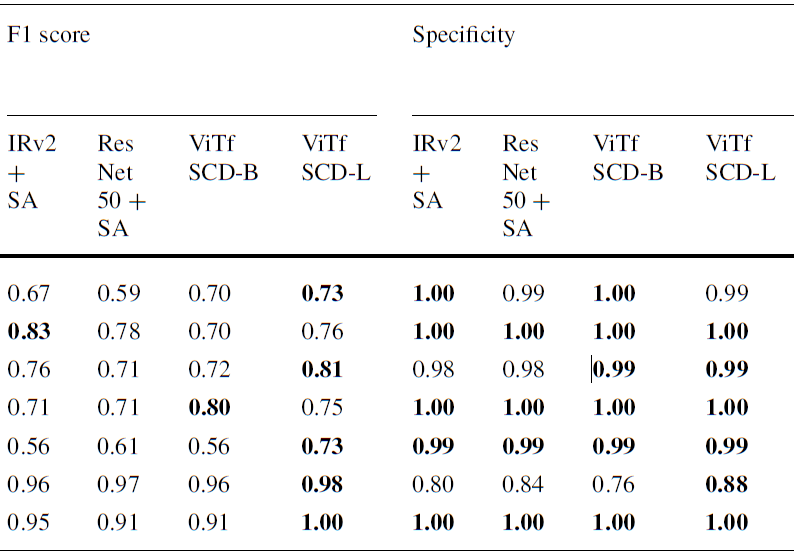
\includegraphics[width=1.00\textwidth]{2/figures/vitpaper1_part2.png}
		\caption[Comparación de resultados de los modelos (f1-socre y specificity)]{Comparación de resultados de los modelos (f1-socre y specificity). \\
		Fuente: \cite{pr_yang2023novelViTscc}. \textit{A Novel Vision Transformer Model for Skin Cancer Classification}.}
		\label{2:fig105}
	\end{center}
\end{figure}

De los resultados, se observó que el modelo ViTfSCD-Large obtuvo el más alto precision, recall, y F1 scores. Además, el mismo modelo obtuvo un accuracy de 94.1\%, siendo el valor más alto, mientras que el modelo ViTfSCD-Base obtuvo 91.4\%.

Finalmente, se realizó una comparación de los modelos a través de su accuracy. En esta última sección, se comparó con otros modelos del estado de arte desarrollados con el conjunto de datos HAM10000. El primero de estos, implementado en 2020 y denominado Efficient-Net logró un accuracy de 92.6\%. También, en el año 2021, se desarrolló un método semi supervisado para la clasificación de imágenes médicas que obtuvo un accuracy de 92.5\%. 

Para esta comparación final, también se consideraron los resultados originales de los modelos IRv2, IRv2 + SA, ResNet50 y ResNet50 + SA junto con los resultados obtenidos en esta investigación. Además, también se realizaron experimentos con los modelos ViT originales (ViT-Base 16 y ViT-Large 16). Los resultados finales muestran que los modelos ViTfSCD-Base y ViTSCD-Large son superiores a sus versiones originales.

\begin{figure}[H]
	\begin{center}
		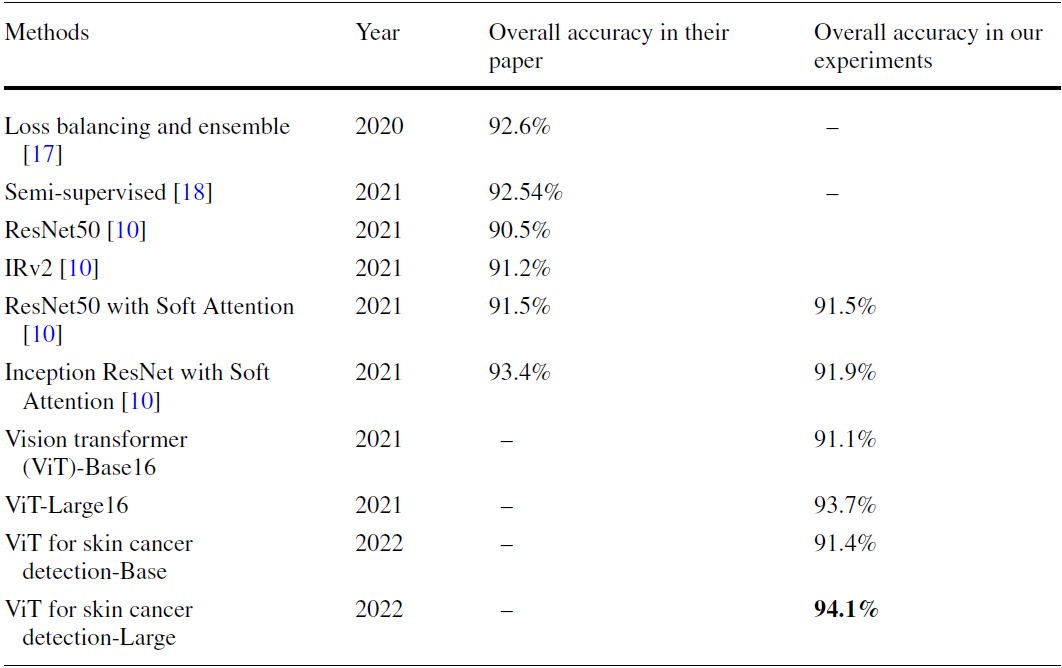
\includegraphics[width=0.90\textwidth]{2/figures/vitpaper1_part3.png}
		\caption[Comparación de resultados según accuracy con el conjunto de datos HAM10000]{Comparación de resultados según accuracy con el conjunto de datos HAM10000. \\
		Fuente: \cite{pr_yang2023novelViTscc}. \textit{A Novel Vision Transformer Model for Skin Cancer Classification}.}
		\label{2:fig106}
	\end{center}
\end{figure}

También se realizaron experimentos con el conjunto de datos DERMOFIT que consta de imágenes de lesiones clínicas de la piel divididas en 10 clases distintas. Los resultados originales con este conjunto de datos muestran que el modelo ResNet50 tuvo mejor desempeño que el modelo de árbol de decisión y KNN. 

Los nuevos experimentos con este conjunto de datos se llevaron a cabo con los modelos ResNet50, IRv2 y ViTfSCD-Base. Los siguientes resultados muestran el desempeño superior del modelo ViTfSCD frente a los demás.

\begin{figure}[H]
	\begin{center}
		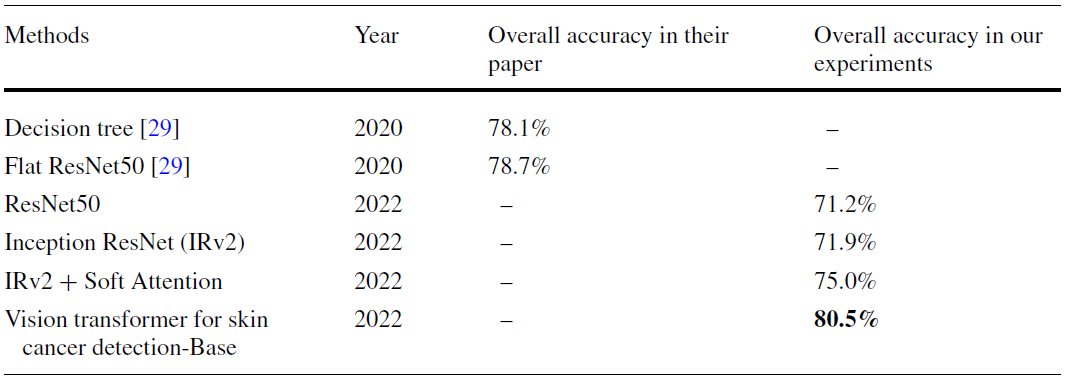
\includegraphics[width=1.00\textwidth]{2/figures/vitpaper1_part4.png}
		\caption[Comparación de resultados según accuracy con el conjunto de datos DERMOFIT]{Comparación de resultados según accuracy con el conjunto de datos DERMOFIT. \\
		Fuente: \cite{pr_yang2023novelViTscc}. \textit{A Novel Vision Transformer Model for Skin Cancer Classification}.}
		\label{2:fig107}
	\end{center}
\end{figure}


\section{Bases Teóricas}
\subsection{Deep Learning}

El Deep Learning o Aprendizaje Profundo es una rama del Machine Learning que conforma varios tipos de algoritmos y enfoques mucho más amplios. Este involucra tratar a los problemas que requiere mayor generalización como lo es la visión por computadora y el reconocimiento de voz. Es decir, estos problemas generales se refieren a problemas que los humanos pueden resolver con facilidad. El Deep Learning involucra al Aprendizaje Supervisado, No Supervisado y el Aprendizaje por Refuerzo. El concepto de “profundidad” se refiere a la característica de sus enfoques en usar muchas capas de redes neuronales artificiales, donde cada una de estas realiza una operación especial, para que en conjunto su complejidad y potencia de resolución de problemas sea mayor. \parencite{bk_hurbans2020grokking}

En el caso de esta investigación, la principal técnica a usar dentro del Deep Learning son las Convoluciones. Esta técnica permite la extracción de características de imágenes para posteriormente realizar su clasificación con respecto a estos. En el proceso de convolución es importante mencionar a los filtros. Estos contienen pesos que son multiplicados por los valores de los pixeles de una imagen, para que finalmente se obtenga un nuevo valor de pixel \parencite{bk_moroney2020aiandml}. A continuación, se presenta un ejemplo gráfico de convolución 2D en una imagen del conjunto de datos Fashion MNIST.

\begin{figure}[H]
	\begin{center}
		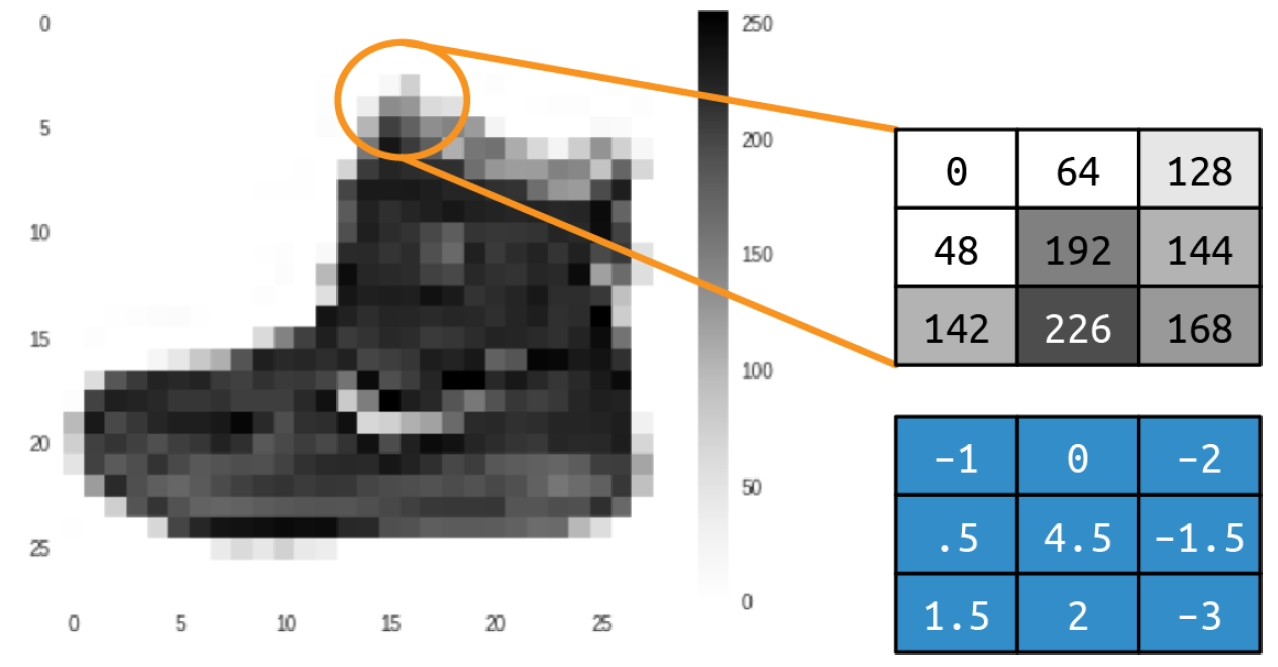
\includegraphics[width=1.00\textwidth]{2/figures/cnn_fash_mnist.png}
		\caption[Convolución de imagen de Fashion MNIST]{Convolución de imagen de Fashion MNIST. \\
		Fuente: \cite{bk_moroney2020aiandml}. \textit{AI and Machine Learning for Coders}.}
		\label{2:fig201}
	\end{center}
\end{figure}

Con un filtro de 3x3 como se muestra en la imagen, se puede modificar el valor del pixel. Este proceso se repite con cada pixel en imagen. Finalmente, se obtiene una imagen nueva conocida como una imagen filtrada. \parencite{bk_moroney2020aiandml} En el ejemplo anterior, el nuevo valor del pixel original 192 será 577, pues este es el resultado de multiplicar, y posteriormente sumar, los pesos del filtro con el valor del pixel y sus vecinos.

Existen distintos tipos de filtros que modifican y otorgan distintos tipos de resultados. Como ejemplo se presentan a continuación las siguientes imágenes.

\begin{figure}[H]
	\begin{center}
		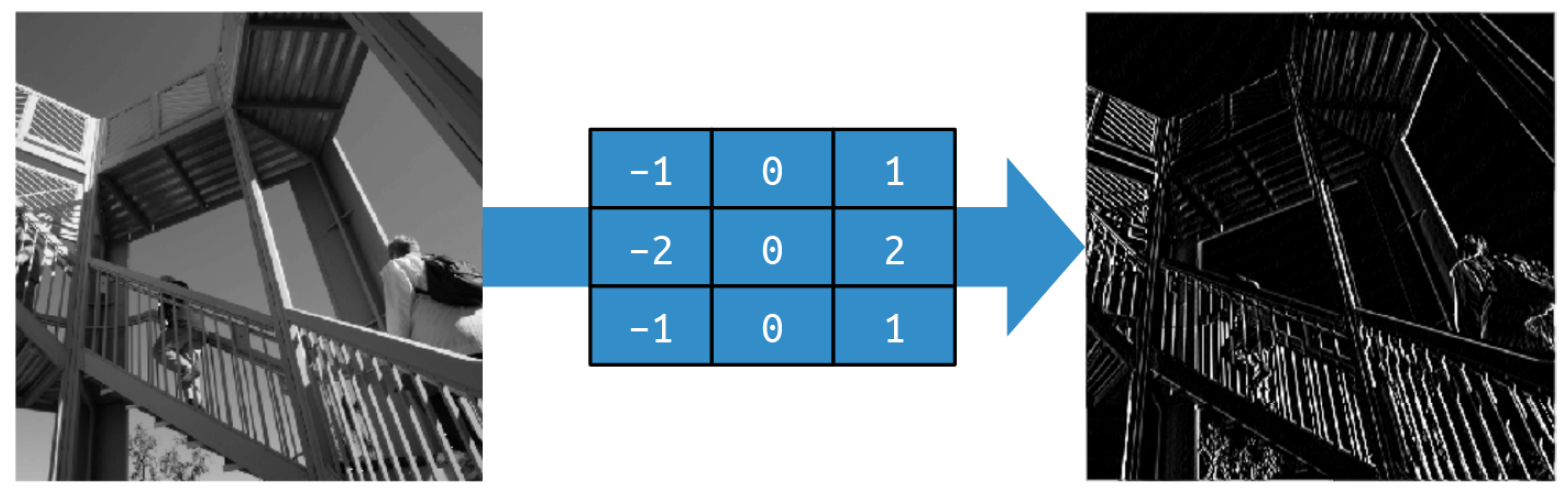
\includegraphics[width=1.00\textwidth]{2/figures/cnn_filtro_vert.png}
		\caption[Convolución de imagen con filtro de líneas verticales]{Convolución de imagen con filtro de líneas verticales. \\
		Fuente: \cite{bk_moroney2020aiandml}. \textit{AI and Machine Learning for Coders}.}
		\label{2:fig202}
	\end{center}
\end{figure}

\begin{figure}[H]
	\begin{center}
		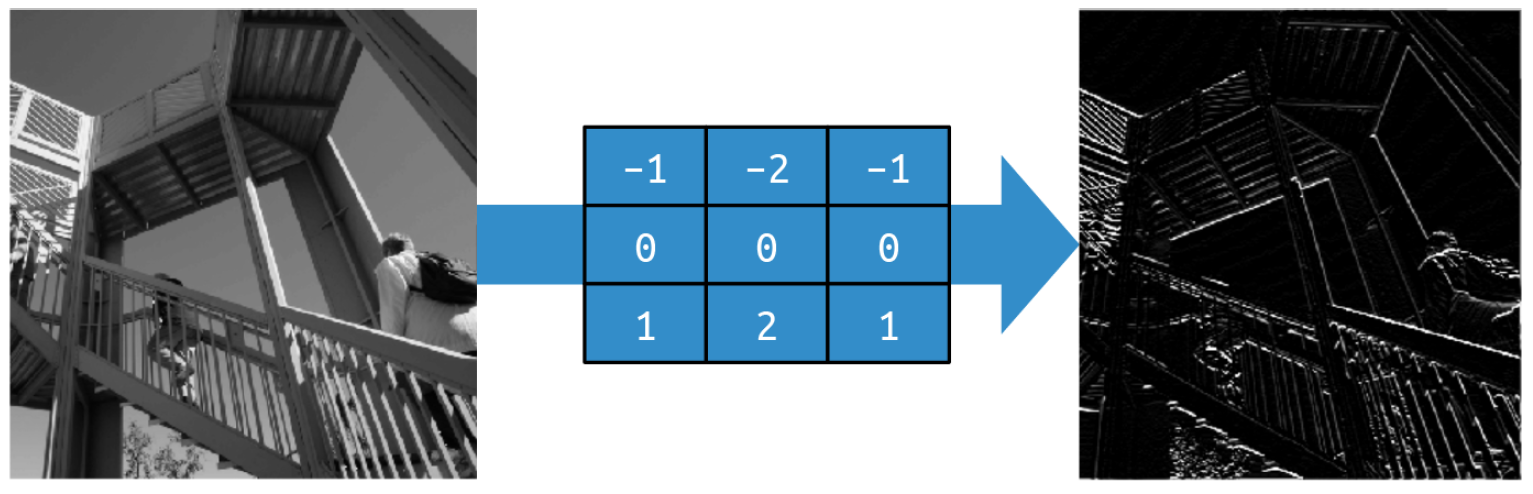
\includegraphics[width=1.00\textwidth]{2/figures/cnn_filtro_hori.png}
		\caption[Convolución de imagen con filtro de líneas horizontales]{Convolución de imagen con filtro de líneas horizontales. \\
		Fuente: \cite{bk_moroney2020aiandml}. \textit{AI and Machine Learning for Coders}.}
		\label{2:fig203}
	\end{center}
\end{figure}

El primer filtro realiza modificaciones a una imagen original para finalmente obtener otra imagen distinta en donde se resaltan las líneas verticales. Caso contrario pasa con el segundo filtro, donde la imagen original es modificada para resaltar sus líneas horizontales. Así, existen distintos tipos de filtros con distintos pesos. Cada uno de estos permite resaltar en las imágenes, a través de modificaciones en sus pixeles, sus características más importantes que serán de utilidad para diferenciar entre una clase u otra de un conjunto de imágenes. También se podría decir que esta técnica de aplicar convoluciones permite reducir la cantidad de información presente en las imágenes, entonces se podría aprender o encontrar un conjunto de filtros específicos capaces de reducir la gran cantidad de información de las imágenes en características que estén relacionadas a sus respectivas etiquetas \parencite{bk_moroney2020aiandml}.

Para reducir la cantidad de información presente en las imágenes, manteniendo al mismo tiempo las características obtenidas por las convoluciones, es necesario aplicar otra técnica entro del mundo del Deep Learning.

El proceso de pooling consiste en eliminar cierta cantidad de pixeles en una imagen, mientras se mantienen las partes resaltantes de la misma. Este proceso normalmente se realiza con agrupaciones de 2x2 en los pixeles de una imagen. Estas agrupaciones también son conocidos como pool. Dentro de cada uno de estas se selecciona el máximo valor de pixel. El proceso se repite con nuevos grupos de pixeles para finalmente obtener una nueva imagen de tamaño considerablemente reducido. \parencite{bk_moroney2020aiandml} A continuación se presenta un ejemplo gráfico.

\begin{figure}[H]
	\begin{center}
		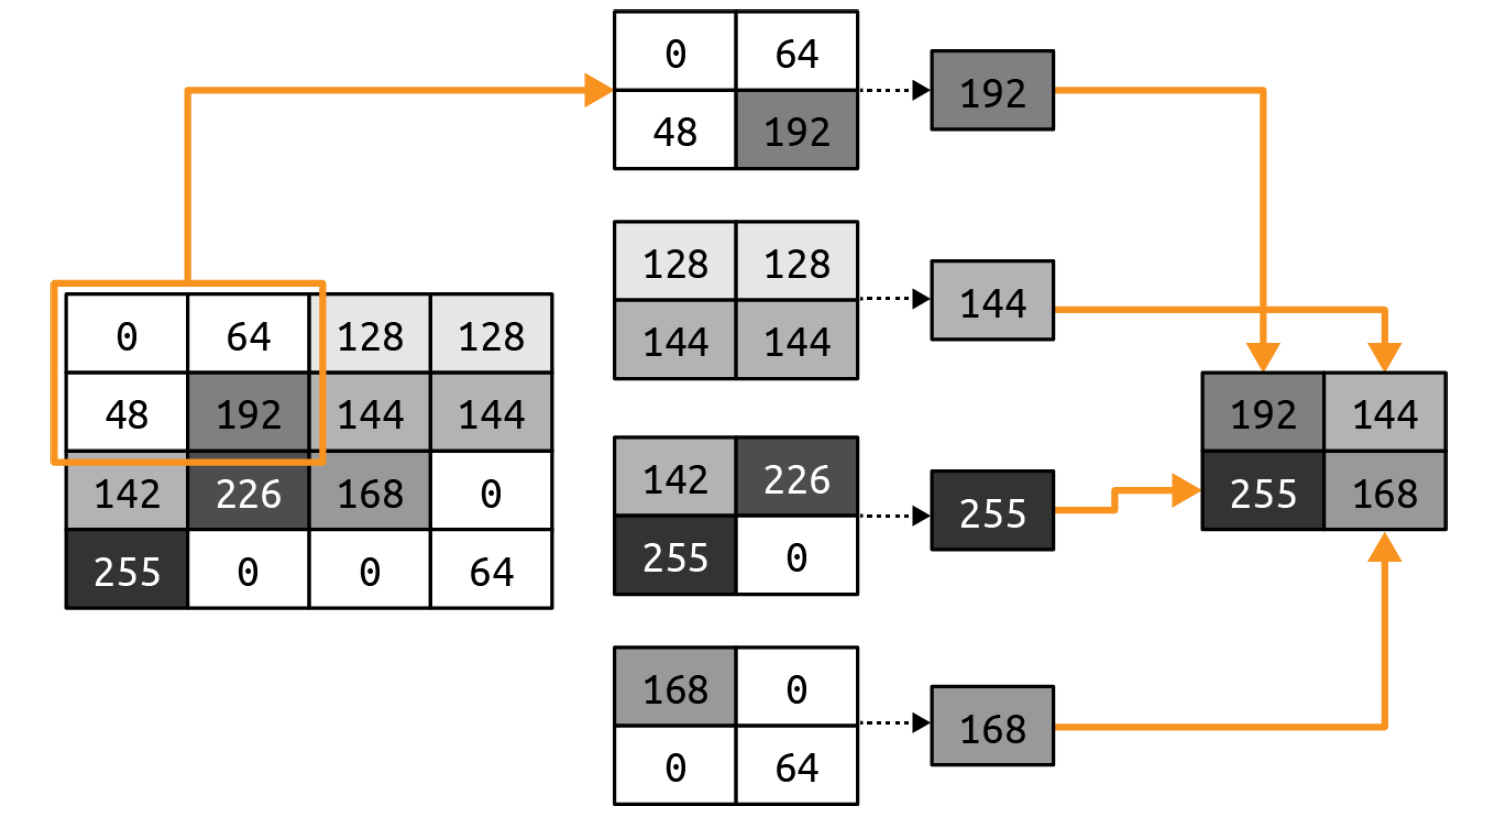
\includegraphics[width=1.00\textwidth]{2/figures/cnn_pool_examp.png}
		\caption[Ejemplo de max-pooling con un pool de 2x2]{Ejemplo de max-pooling con un pool de 2x2. \\
		Fuente: \cite{bk_moroney2020aiandml}. \textit{AI and Machine Learning for Coders}.}
		\label{2:fig204}
	\end{center}
\end{figure}

La imagen original de 4x4 pixeles, luego de ser aplicado el proceso de pooling, se obtiene una imagen reducida de 2x2 pixeles. De manera general, la imagen redujo a la cuarta parte de la cantidad original de pixeles.

Con estas dos técnicas del Deep Learning se han ido desarrollando distintas arquitecturas de redes neurales en la última década. Algunas más complejas y con más capas que otras. Cada una de estas han logrado desempeñarse de forma satisfactoria con el conjunto de datos con el que se han entrenado, demostrando el gran potencial de la redes neuronales convolucionales o CNN.

Algunas de las arquitecturas más conocidas y que han sido usadas en gran variedad de investigaciones son los VGG, ResNet, Inception y DenseNet.

La arquitectura VGG o VGGNet es una red neuronal artificial con una profundidad de 16 o 19 capas (dependiendo de la versión que se analice) y usa pequeños filtros de convolución de tamaño 3x3 a través de estas. Este modelo participó en el ImageNet Challenge 2014, donde logró el primer puesto en las tareas de localización y segundo puesto en clasificación. Además, tiene la alta capacidad de generalización en otros conjuntos de datos, es decir, es capaz de obtener buenos resultados con imágenes distintas a las usadas para su entrenamiento. \parencite{pr_simonyan2015vdcn}

Otra arquitectura bastante difundida en el mundo del Deep Learning y las CNN es ResNet. Esta arquitectura nace de la premisa del aumento de la dificultad de entrenar las redes neuronales profundas. Con el objetivo de facilitar este proceso se añade a las ya conocidas CNN el concepto de residual, para obtener redes residuales que sean mucho más fáciles de optimizar y capaces de obtener mejor desempeño a más grande sea la profundidad de la red. El modelo tuvo 152 capas, ocho veces más grande que las arquitecturas VGG, y fue evaluada con el conjunto de datos ImageNet. \parencite{pr_he2016deepres}

Inception es una arquitectura que obtuvo un alto desempeño en las tareas de clasificación y detección en el ImageNet Large-Scale Visual Recognition Challenge 2014 (ILSVRC14). La principal distinción de este modelo es el uso de los recursos informáticos a través de la red. Esto significa que mientras más aumente la complejidad del modelo a través de su profundidad, los recursos computacionales no variarán a gran escala como se esperaría. Esto se logra a través del uso de módulos de Inception en algunas capas de la arquitectura en general. Los distintos módulos se encuentran apilados unos sobre otros y con algunas capas max-pooling. Dentro de esta arquitectura, se tiene a GoogLeNet, que no es más que una versión de Inception de 22 capas (este modelo fue el presentado a ILSVRC14). \parencite{pr_szegedy2015goingdwc}

DenseNet nace con la premisa de que las CNN pueden obtener mejores desempeños si se tienen conexiones cortas entre las capas cerca de la entrada y salida de la red. La propuesta de esta red consiste en establecer una conexión de cada capa con todas las demás capas de la misma red. Esto trae grandes ventajas como la reducción del problema de gradiente de fuga, fomenta la reutilización de características extraídas en previas capas, además de disminuir la cantidad de parámetros. El modelo fue evaluado con los conjuntos de datos CIFAR-10, CIFAR-100, SVHN e ImageNet para la tarea de reconocimiento de objetos. \parencite{pr_huang2016densconn} A continuación, se muestra una representación de DenseNet con 5 capas.

\begin{figure}[H]
	\begin{center}
		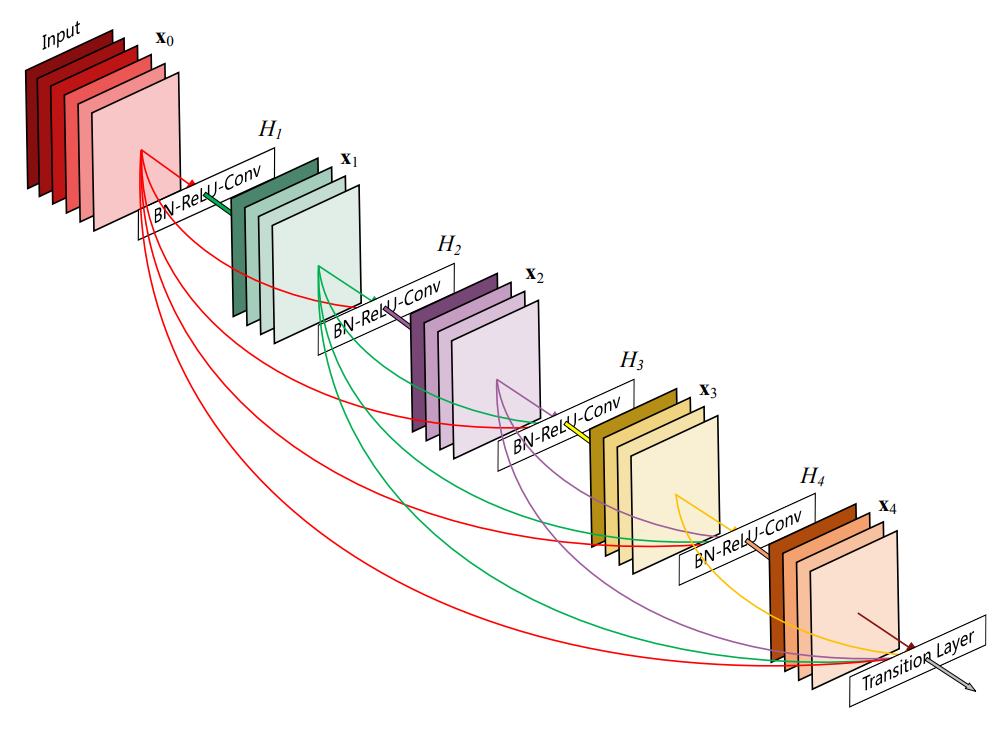
\includegraphics[width=1.00\textwidth]{2/figures/densenet_5lay.png}
		\caption[DenseNet con 5 capas]{DenseNet con 5 capas. \\
		Fuente: \cite{pr_huang2016densconn}. \textit{Densely Connected Convolutional Networks}.}
		\label{2:fig205}
	\end{center}
\end{figure}

Las tareas relacionadas al procesamiento de imágenes como la segmentación, detección de objetos y clasificación es actualmente dominada por las redes neuronales convolucionales explicadas anteriormente; sin embargo, gracias al gran avance y divulgación de los modelos basados en Transformers, se ha visto el surgimiento de un nueva clase de arquitecturas que prometen mejorar el desempeño de los actuales modelos dominantes: los Vision Transformer (ViT).

Según la investigación original presentada por \cite{pr_dosovitskiy2021animageisworth}, los modelos Transformer, dominantes actuales en tareas de procesamiento de lenguaje natural (NLP), se han convertido en el modelo predilecto cuando se trata de manejo de texto, esto debido a su capacidad de utilizar los recursos computacionales de forma eficiente y su escalabilidad, permitiendo así obtener modelos de; por ejemplo, 100 mil millones de parámetros.

A diferencia de las tareas de NLP, la visión por computadora tuvo mayores problemas para adaptar este nuevo tipo de arquitecturas a sus tareas específicas.

Los primeros intentos se basaban en usar la capacidad de self-attention de los Transformer y combinarlo con los dominantes modelos CNN. Estos intentos de obtener los excelentes resultados de los Transformer en las tareas de visión por computadora no obtenían los resultados de los modelos de mayor desempeño como son los basados en la arquitectura de ResNet.

Debido a esto y al gran potencial que tenían las arquitecturas basadas en Transformers, propusieron el uso de estas arquitecturas aplicadas de forma directa a imágenes; es decir, aplicando la menor cantidad de cambios antes de ingresar al mismo Transformer. El proceso exacto de cómo funciona su arquitectura se explicará más adelante.

La gran ventaja de este nuevo tipo de modelos se basa en la cantidad de datos con la que es entrenado. 

En el caso de usar una pequeña cantidad de imágenes para el entrenamiento se obtienen resultados no favorables, llegando a tener un bajo rendimiento comparado a los modelos basados en CNN. Sin embargo, al realizar su entrenamiento con una mayor cantidad de datos, los Vision Transformer (como se le nombró a este nuevo tipo de arquitectura) obtuvieron mejores resultados que los modelos dominantes en las mismas tareas de visión por computadora.

A diferencia de los Transformer dedica a las tareas de NLP que reciben como entrada token embeddings de una sola dimensión, las imágenes son de dos dimensiones (H, W) y una cantidad de canales (C), lo que dificulta su ingreso directo a este tipo de arquitecturas. Es por esto que es necesario aplicar una división de las imágenes en patches 2D que posteriormente serán aplanados e ingresados al Transformer como haría normalmente los token embeddings.

Estos patches deben tener un tamaño constante P, es decir que se deben obtener divisiones de las imágenes de tamaño P x P. Esto conlleva a que el número de patches final sea igual a $N = HW / P^2$.

Una vez se tienen los N patches, se realiza su aplanamiento y, posteriormente, se mapean en D dimensiones (tamaño del vector latente usado en el Transformer) a través de una proyección lineal capaz de ser entrenada.

Ya obtenidos estos patch embedding, se añade uno nuevo pero con la capacidad de ser aprendible. Estos se agrupan en una secuencia que ingresarán posteriormente al Transforme encoder. Cabe resaltar que, luego de pasar por el encoder, este último embedding añadido representará a la imagen.

A los ya mencionados patch embedding también se le agrega otro tipo de embedding capaz de mantener información relacionada a la posición de cada patch. Estos embedding son 1D y aprendibles. Finalmente, estos serán ingresados juntos con los originales embeddings a Transformer encoder.

En la parte final de la arquitectura se tiene un MLP con la principal tarea de realizar la clasificación de las imágenes. Este MLP consta de una sola capa oculta en la etapa de entrenamiento inicial del modelo, y con una sola capa lineal en la etapa de fine-tuning.

El bloque de Transformer encoder está compuesto por distintos bloques como los multi headed self attention (MSA), MLP y los Layernorm (LN). Estos distintos bloques se van alternando de forma específica, introduciendo además conexiones residuales luego del MSA y MLP.

Toda la arquitectura de los ViT se puede resumir con la siguiente imagen.

\begin{figure}[H]
	\begin{center}
		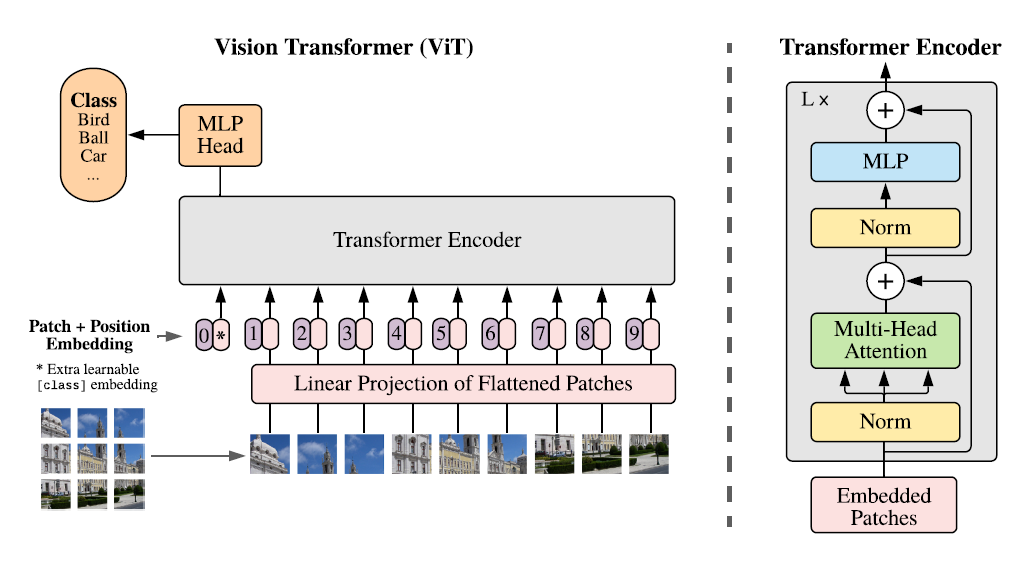
\includegraphics[width=1.00\textwidth]{2/figures/vit_arquitecture.png}
		\caption[Arquitectura del modelo ViT]{Arquitectura del modelo ViT. \\
		Fuente: \cite{pr_dosovitskiy2021animageisworth}. \textit{AN IMAGE IS WORTH 16X16 WORDS: TRANSFORMERS FOR IMAGE RECOGNITION AT SCALE}.}
		\label{2:fig206}
	\end{center}
\end{figure}


\subsection{Nódulos Tiroideos}
Para entender qué es un nódulo tiroideo, primero se debe sabes qué es la tiroides. Este es una glándula localizada en el cuello del cuerpo humano que se encarga de producir hormonas que regulan el metabolismo. Los nódulos que aparecen en esta glándula son los más comunes, y se generan debido a un excesivo crecimiento de las células en esa área, estos pueden ser de textura dura o quísticas. \parencite{pr_deng2022autclass}

La siguiente figura muestra a la glándula en una imagen tomográfica.

\begin{figure}[H]
	\begin{center}
		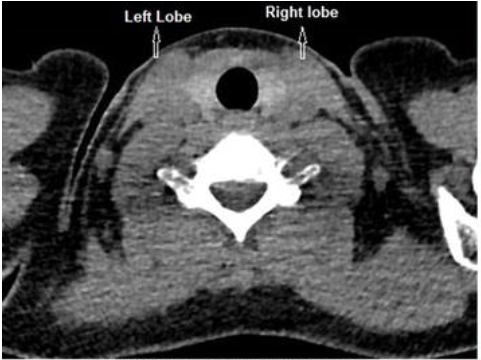
\includegraphics[width=0.75\textwidth]{2/figures/gland_thyroid.png}
		\caption[Imagen tomográfica de glándula de tiroides]{Imagen tomográfica de glándula de tiroides. \\
		Fuente: \cite{pr_binboga2019thyroid}. \textit{Thyroid Anatomy}.}
		\label{2:fig206}
	\end{center}
\end{figure}

\cite{pr_shin2016ultradiag} mencionan que existen algunas características de los nódulos en la tiroides que pueden ser analizados para realizar una clasificación si es de carácter benigno o maligno. A continuación, se presentan aquellos más resaltantes.

El tamaño de nódulos en ciertos casos puede determinar el tipo con el que se está tratando; sin embargo, esto no está debidamente comprobado, a pesar de que normalmente el riesgo de ser maligno de un nódulo es más alto en aquellos de mayor tamaño. Esto principalmente se debe a que los nódulos benignos también pueden llegar a un tamaño considerable, pero con una mayor cantidad de tiempo. Lo que sí puede significar un probable nódulo maligno es un rápido crecimiento de un nódulo sólido.

El contenido interno de un nódulo está determinado por el ratio entre su parte quística y su parte sólida. Los nódulos malignos con contenido sólido poseen mayor riesgo de ser malignos que aquellos con contenido parcialmente quístico.

La ecogenicidad de los nódulos se mide de acuerdo al nivel de brillo en las imágenes de ultrasonido con respecto a otras partes de la imagen. Esto quiere decir que un nódulo es hipoecoico si su nivel de brillo en la imagen es menor con respecto a otra parte de la imagen, específicamente se compara con el músculo anterior del cuello o el parénquima tiroideo. La mayoría de los tumores tiroideos son hipoecoicos, y existe mayor riesgo de que los nódulos con la misma característica sean malignos.

La forma y orientación de los nódulos también pueden determinar si son o no malignos. La manera en que los nódulos malignos crecen es de manera centrífuga y a través del plano del tejido, al igual que los benignos; sin embargo, estos crecen de manera paralela. La forma redonda u ovoide de los nódulos se encuentra en aquellos de carácter benigno; sin embargo, no son propias de este. Una característica mucho más específica de los nódulos de carácter malignos es su orientación no paralela, es decir, son más altos que anchos.

Finalmente, el margen de los nódulos también puede dar información del tipo con el que se trata. Una característica que sugiere que un nódulo es maligno es un margen espiculado o micro tubulado.



\section{Marco Conceptual}
\subsection{Inteligencia Artficial}
Definir a la Inteligencia Artificial llega a ser complicado, esto debido a la dificultad que se tiene en definir lo que en verdad es inteligencia. Algunos grandes personajes pensaban de la inteligencia como la ambición, mientras que otros mencionaban a la imaginación como gran impulsador de la inteligencia. También lo consideraban como la capacidad de adaptarse a los cambios. Estas definiciones hacen pensar que no existe un consenso claro de lo que es la inteligencia, menos aun de la Inteligencia Artificial; sin embargo, en términos generales, se puede calificar de “Inteligencia Artificial” a todo aquel sistema sintético que muestra algún tipo de comportamiento “inteligente”. Esto quiere decir que se puede considerar como IA a todo a aquellos que simule los sentidos naturales como el visión o audición, incluso a la capacidad de algunos sistemas de aprender de forma autónoma según su entorno lo requiera. \parencite{bk_hurbans2020grokking}

\subsection{Perceptrón}
Inventado por Frank Rosenblatt en 1957, el Perceptrón es la unidad básica de una red neuronal e incluso es considerado como la más simple red neuronal artificial (ANN). \parencite{bk_geron2022handml}

El Perceptrón se muestra en la Figura \ref{2:fig207-2}.

\begin{figure}[H]
	\begin{center}
		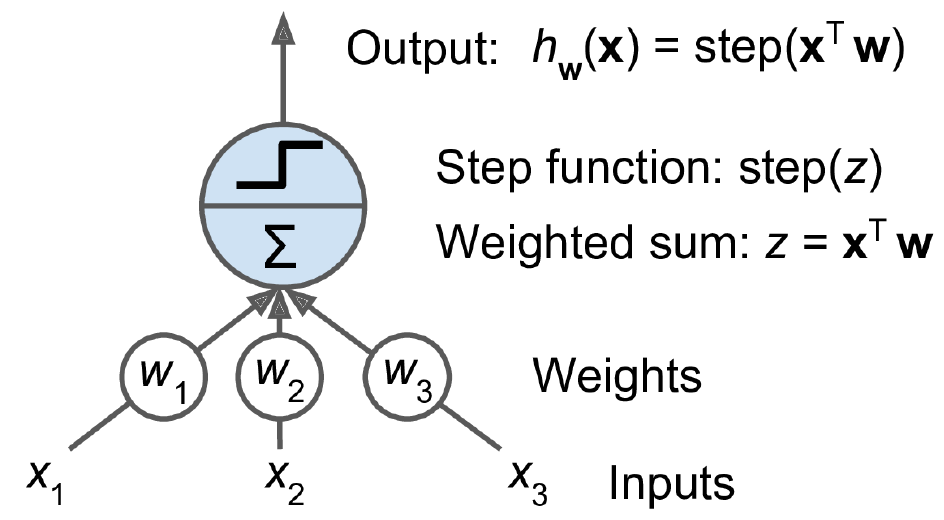
\includegraphics[width=0.75\textwidth]{2/figures/perceptron.png}
		\caption[Perceptrón]{Perceptrón. \\
		Fuente: \cite{bk_geron2022handml}. \textit{Hands-on machine learning with Scikit-Learn, Keras, and TensorFlow}.}
		\label{2:fig207-2}
	\end{center}
\end{figure}


\subsection{Perceptrón Multicapa}
Un Multi-Layer Perceptron (MLP) consiste en la unión de varios perceptrones, con la característica de estar organizados por capas. Existe una capa de entrada y otra de salida, todas las capas, a excepción de la salida, contiene una neurona adicional llamada bias. \parencite{bk_geron2022handml}

Una representación gráfica de un MLP se muestra en la Figura \ref{2:fig208}.

\begin{figure}[H]
	\begin{center}
		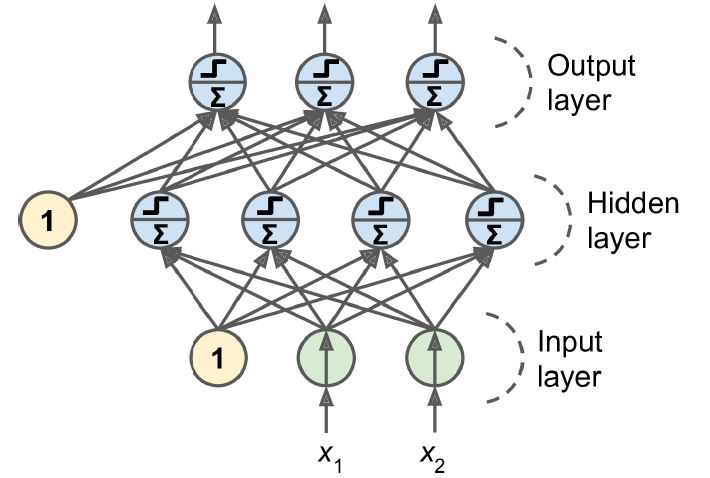
\includegraphics[width=0.77\textwidth]{2/figures/mlp.png}
		\caption[Perceptrón Multicapa]{Perceptrón Multicapa. \\
		Fuente: \cite{bk_geron2022handml}. \textit{Hands-on machine learning with Scikit-Learn, Keras, and TensorFlow}.}
		\label{2:fig208}
	\end{center}
\end{figure}


\subsection{Machine Learning}
El Aprendizaje Automático o Machine Learning es considerado como una ciencia y arte de dar instrucciones a una computadora para que pueda aprender por sí sola de una data. \parencite{bk_geron2022handml}

En la Figura \ref{2:fig209} se presenta el enfoque tradicional del Machine Learning.

\begin{figure}[H]
	\begin{center}
		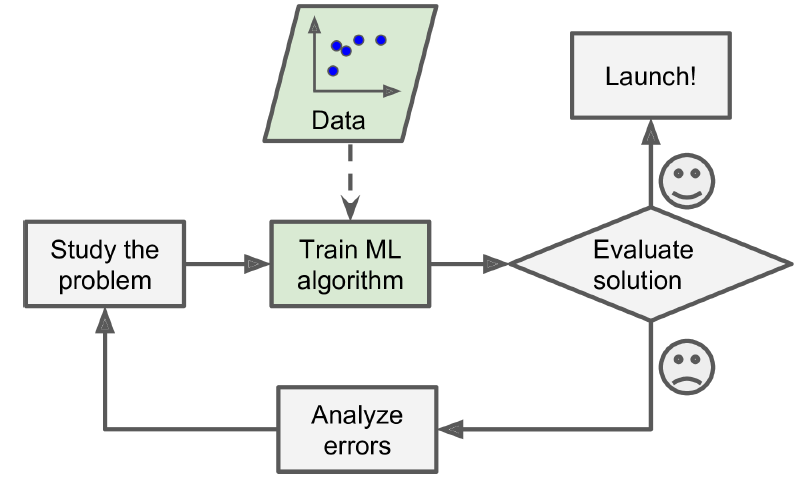
\includegraphics[width=0.75\textwidth]{2/figures/enfoque_ml.png}
		\caption[Enfoque del Machine Learning]{Enfoque del Machine Learning. \\
		Fuente: \cite{bk_geron2022handml}. \textit{Hands-on machine learning with Scikit-Learn, Keras, and TensorFlow}.}
		\label{2:fig209}
	\end{center}
\end{figure}

\begin{comment}

\subsection{Ecografía y las imágenes de ultrasonido}
Según \cite{pr_herrera2017diseimp}, la ecografía, que es una técnica de diagnóstico en donde se usan imágenes generadas por ultrasonido, es comúnmente desarrollado en las áreas de cardiología, ginecología, y otras más relacionadas. La popularidad de esta técnica se basa en la capacidad de las imágenes de alta calidad que se obtienen de este proceso, además de no ser un método invasivo o de radiación como muchos otros de su tipo.

Los sistema encargados de extraer las imágenes de ultrasonido son compuestos de distintas sensores que generan ondas de sonido para posteriormente analizar la respuesta de la interacción física con el campo de interés. Estas señales recibidas de regreso son digitalizados por una parte electrónica delantera que también transforman estos datos crudos en la imagen final. El funcionamiento de este proceso depende de la configuración de los sensores, el método usado para obtener las imágenes y las características de área de interés. \parencite{pr_camacho2022ultrasonicimg}

Algunas imágenes de ultrasonido de nódulos tiroideos se muestran en la Figura \ref{2:fig210}.

\begin{figure}[H]
	\begin{center}
		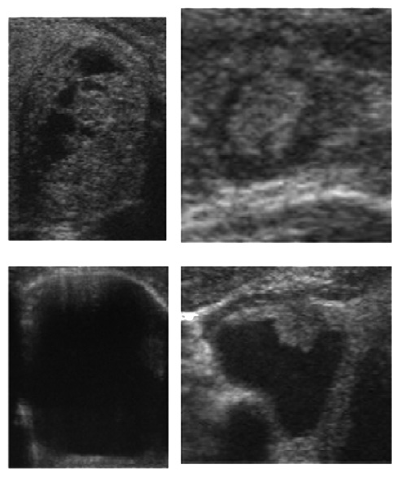
\includegraphics[width=0.40\textwidth]{2/figures/imagenes_ultrasonido_originales.png}
		\caption[Imágenes de ultrasonido de nódulos tiroideos]{Imágenes de ultrasonido de nódulos tiroideos. \\
		Fuente: \cite{pr_JERBI2023autoclassViTGAN}. \textit{Automatic classification of ultrasound thyroids images using vision transformers and generative adversarial networks}.}
		\label{2:fig210}
	\end{center}
\end{figure}


\subsection{Transfer Learning}
\cite{bk_geron2022handml} nos menciona que el Transfer Learning o Transferencia de Aprendizaje es un técnica usada en el campo de Deep Learning que permite el uso de algunas capas de un modelo ya definido y entrenado previamente en un nuevo modelo que necesite ser entrenado en una tarea similar al que se desarrolla el modelo original. Las capas destinadas al reuso son normalmente las más cercanas a la entrada o también conocidas como capas inferiores. El beneficio de usar esta técnica radica en dos puntos importantes: cantidad de datos requeridos y velocidad de entrenamiento del modelo; es decir, la cantidad de datos que se deben usar para entrenar un modelo de alto desempeño se reduce considerablemente, mientras que el tiempo requerido para terminar este proceso es menor comparándolo a si lo entrenaran desde cero.

Para que esta técnica funcione debidamente, las capas más cercanas a la salida, conocidas también como capas de alto nivel, deben ser reemplazadas, esto debido a que son más específicas de las tareas del modelo original. Esto también incluye a la capa final, ya que posiblemente no tenga la cantidad de salidas necesarias para completar satisfactoriamente la nueva tarea.

En la Figura \ref{2:fig211} se presenta de forma gráfica la técnica.

\begin{figure}[H]
	\begin{center}
		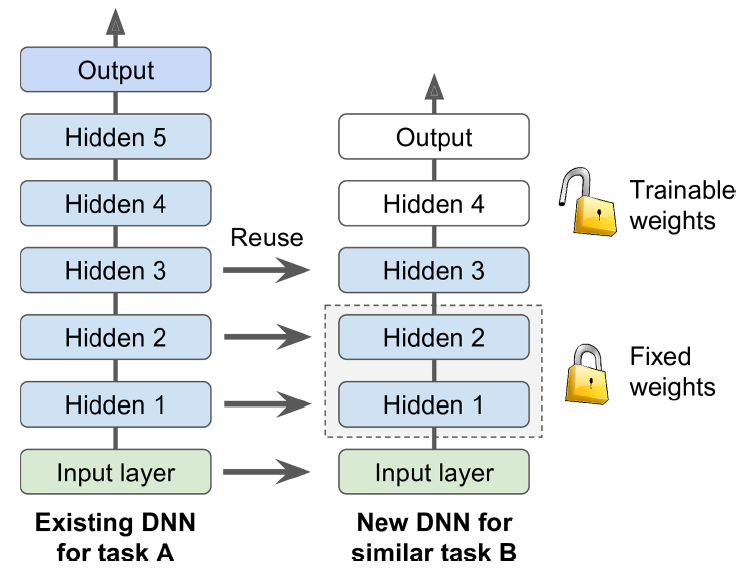
\includegraphics[width=0.70\textwidth]{2/figures/transfer_learning.PNG}
		\caption[Ejemplo de Transfer Learning]{Ejemplo de Transfer Learning. \\
		Fuente: \cite{bk_geron2022handml}. \textit{Hands-on machine learning with Scikit-Learn, Keras, and TensorFlow}.}
		\label{2:fig211}
	\end{center}
\end{figure}


\subsection{Data Augmentation}

Según \cite{bk_geron2022handml} el Aumento de Datos o Data Augmentation es una técnica de regularización que permite reforzar la cantidad de muestras en un conjunto de datos. Esto se realiza a través de la generación de nuevas instancias similares a los originales; es decir, las personas no deberían ser capaces de diferenciar una imagen generada de una del propio conjunto de datos.

Para generar estas nuevas muestras, normalmente se aplican diferentes transformaciones a las instancias del conjunto de datos original. Estas transformaciones pueden ser; por ejemplo, una simple rotación o recorte de la imagen, siempre y cuando no altere por completo su sentido como es el caso de voltear una imagen de texto de forma horizontal. 

El principal beneficio de esta técnica es que permite reducir el sobreajuste de los modelos entrenados. 

En la Figura \ref{2:fig212} se muestran algunas transformaciones que se pueden hacer al aplicar el Aumento de Datos. 

\begin{figure}[H]
	\begin{center}
		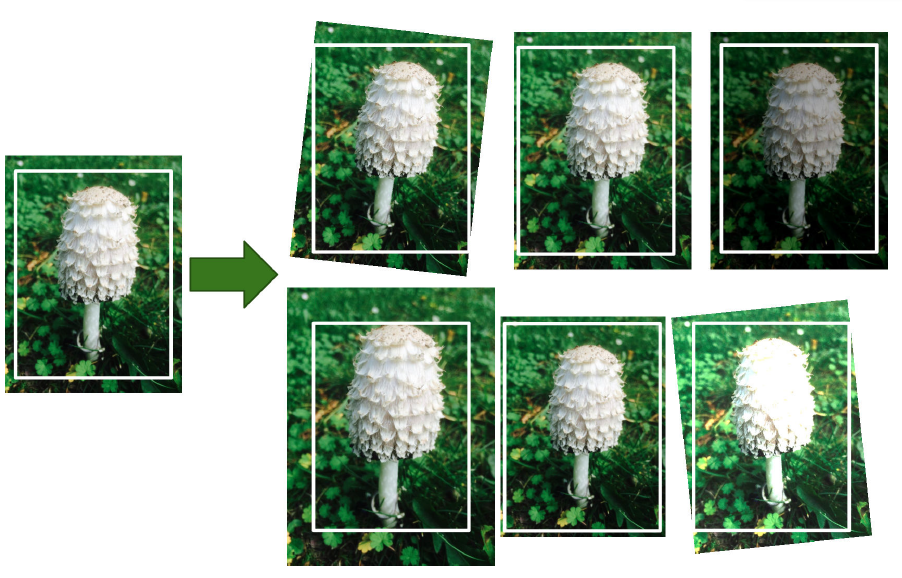
\includegraphics[width=0.85\textwidth]{2/figures/data_aug.PNG}
		\caption[Ejemplo de Data Augmentation]{Ejemplo de Data Augmentation. \\
		Fuente: \cite{bk_geron2022handml}. \textit{Hands-on machine learning with Scikit-Learn, Keras, and TensorFlow}.}
		\label{2:fig212}
	\end{center}
\end{figure}

\end{comment}

\section{Hipótesis}
\subsection{Hipótesis General}
HG: \newcommand{\HipotesisGeneral}{
A través del diseño de un modelo de Deep Learning se logra diagnósticar lo nódulos tiroideos a través de imágenes de ultrasonido.
}
\HipotesisGeneral


\subsection{Hipótesis Específicas}
\newcommand{\Hone}{
Las mejores características del conjunto de datos son usadas para entrenar y evaluar  modelos permiten un mejor desarrollo del modelo de Deep Learning.
}
\newcommand{\Htwo}{
Las técnicas de preprocesamiento a aplicar a las imágenes de ultrasonido del conjunto de datos mejora el desempeño del modelo de Deep Learning.
}
\newcommand{\Hthree}{
Las métricas de evaluación de rendimiento de los modelos de Deep Learning logra una correcta comparación de modelos en la tarea de clasificación de imágenes de ultrasonido.
}
\newcommand{\Hfour}{
    Las arquitecturas de Deep Learning con más alto desempeño en la clasificación de imágenes de ultrasonido demuestran superioridad frente a los demás modelos.
}

\begin{itemize}
	\item HE1: {\Hone}
	\item HE2: {\Htwo}
	\item HE3: {\Hthree}
	\item HE4: {\Hfour}
\end{itemize}

%\chapter{Metodología de la Investigación}
\section{Diseño de la investigación}
Según \cite{bk_sampieri2014metodologia} el manipular y encontrar una relación de causa-efecto entre las variables independientes y dependientes son propias de los diseños experimentales.

En el caso de la presente investigación se tiene un diseño experimental porque se pretende establecer la relación entre modelos y técnicas de Deep Learning con el pre-diagnóstico de nódulos tiroideos, esto a través de imágenes de ultrasonido. 

\subsection{Tipo de la investigación}
Ya definido el diseño que tendrá la investigación, se consideró al tipo experimental puro para seguir en la presente investigación, esto ya que la variable independiente (técnicas, modelos y herramientas de Deep Learning) será manipulada constantemente con el fin de encontrar una relación de causalidad ideal con la variable dependiente. Es decir, todo lo relacionado con el Deep Learning será manipulado reiteradas veces con el objetivo de encontrar el impacto en el pre-diagnóstico de nódulos tiroideos. La manipulación en las técnicas o modelos de Deep Learning también incluye a la de la data a usar, ya que se aplicarán diversas técnicas para realizar una limpieza y extracción de características que ayudarán a la posterior elaboración de un algoritmo de diagnóstico asistido.

\subsection{Enfoque de la investigación}
Según \cite{bk_sampieri2014metodologia} el enfoque que sigue una forma secuencial donde no se puede evitar ningún paso, y se usan herramientas estadísticas para realizar mediciones, es el enfoque cuantitativo. 

La presente investigación tiene un enfoque cuantitativo, esto dado que la variable independiente usa valores numéricos y/o estadísticos para su medición. Los resultados de la variable de Deep Learning deberán ser medidos a través de valores numéricos y, en mayor medida, estadísticos.

\subsection{Población}
La población consiste en imágenes de ultrasonido de la glándula de tiroides con presencia de nódulos. Estas imágenes fueron recolectadas de 2421 pacientes por el Zhujiang Hospital of Southem Medical University y debidamente validadas por los comités de ética institucionales en China.

\subsection{Muestra}
La muestra consiste en 3493 imágenes de ultrasonido de la glándula de tiroides recopiladas de 2421 pacientes.

\section{Metodología de Implementación de la Solución}
La metodología por seguir para implementar un modelo de Deep Learning está basado en gran medida en el conocido ciclo de vida de desarrollo de modelos de Inteligencia Artificial, del cual gran parte de los antecedentes mostrados anteriormente siguen con algunas variaciones. 

En el presente caso, se pretende desarrollar un modelo de Deep Learning capaz de brindar ayuda en el diagnóstico médico; por tal motivo, se optó por basar metodología de esta investigación en la de \cite{pr_monroy2021disvc}, modificándolo en cierta medida en el contexto de nódulos tiroideos e imágenes de ultrasonido. En la Figura \ref{3:fig301} se presenta de forma gráfica la metodología a seguir.

\begin{figure}[H]
	\begin{center}
		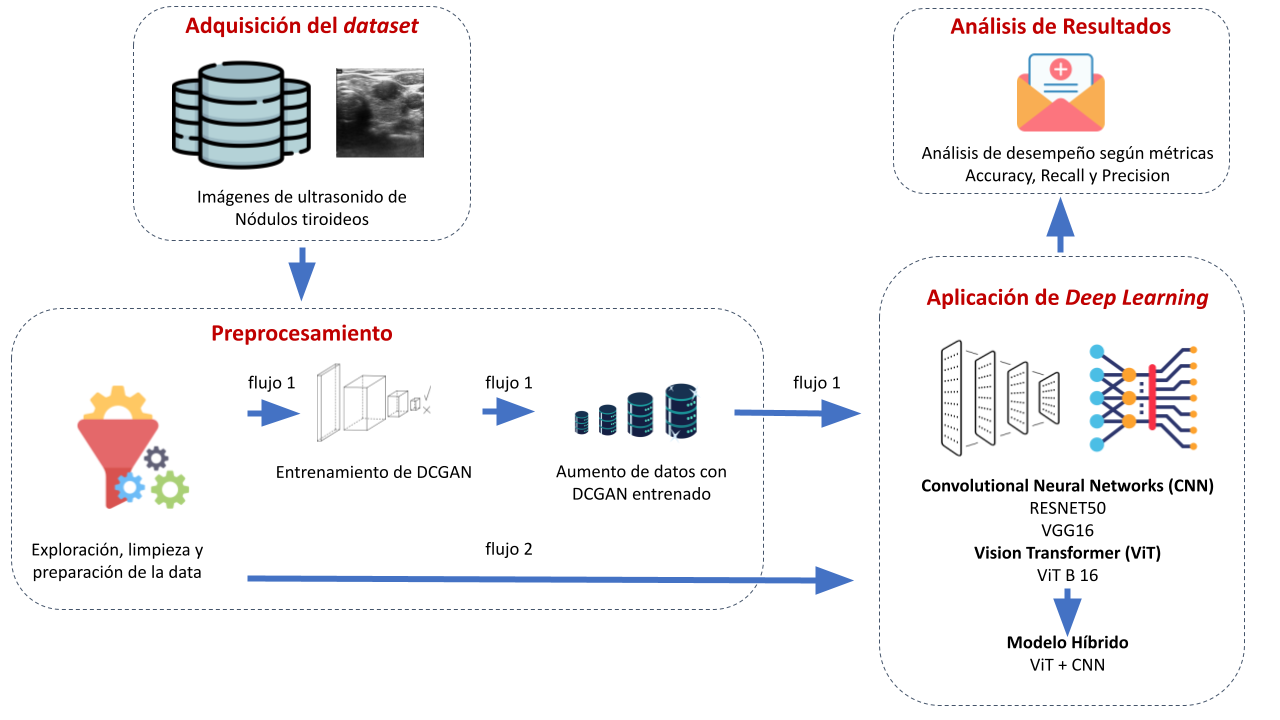
\includegraphics[width=1.00\textwidth]{3/figures/metod_classthy1.png}
		\caption[Metodología de implementación]{Metodología de implementación. \\
		Fuente: Elaboración propia.}
		\label{3:fig301}
	\end{center}
\end{figure}

La adquisición del conjunto de datos, es decir, imágenes de ultrasonido, consiste en la búsqueda y revisión de las bases de datos sobre imágenes de nódulos tiroideos, donde finalmente se seleccionará y descargará la de mayor utilidad. La base de datos debe cumplir con ciertos requerimientos para realizar un posterior entrenamiento del modelo que otorgue buenos resultados. Las imágenes deben ser debidamente etiquetadas según el carácter del nódulo al que representen, es decir, se debe indicar si cada una de las imágenes pertenece a la categoría benigno o maligno. Además, para evitar discrepancias entre calidad de imágenes en futuras evaluaciones, el conjunto de datos debe poseer imágenes de distintas instituciones de salud y de distintas calidades. Esto permitirá que el modelo entrenado no dependa de la una alta o baja calidad de las imágenes para realizar una correcta predicción. Finalmente, la cantidad de datos debe ser relativamente alta con el fin de aumentar la capacidad de generalización del modelo y evitar posibles sobreajustes o bajo rendimiento.  

En la etapa de preprocesamiento, se realizará en primera instancia una exploración del conjunto de datos con el fin de entender su composición y las características a mejorar; por ejemplo, un posible desbalanceo de clases o presencia de imágenes corruptas o sin etiquetar. Posteriormente, se realizará limpieza datos en caso de imágenes corruptas o de nula utilidad. Además, se usarán técnicas de Aumento de Datos en la situación de desbalanceo de datos, con el fin de evitar una baja generalización y sobreajuste en la clase mayoritaria. Además, se aplicará un reescalado y normalización en las imágenes destinadas al entrenamiento del modelo con el objetivo de reducir la complejidad computacional y así obtener menor tiempo de ejecución.

Una vez se tenga la data ya preprocesada, una parte de este se usará para el entrenamiento de modelos de Deep Learning. Inicialmente, se planea usar algunos de los diversos tipos y arquitecturas de Redes Neuronales Convolucionales (CNN), específicamente los más utilizados en este tipo de tareas como lo son VGG y ResNet, pues son ideales para la extracción de características de las imágenes, facilitando así el proceso final de clasificación. Además, se desarrollarán modelos basados en arquitecturas de Vision Transformer debido al potencial que han demostrado en anteriores investigaciones. Finalmente, también se realizará el desarrollo de modelos híbridos de CNN con Vision Transformer. %similares a los descritos por \cite{pr_JERBI2023autoclassViTGAN}.

Cada uno de los modelos será probado en la parte restante de la data, específicamente en la data de prueba o test. De aquí se obtendrán las predicciones de los modelos clasificando las imágenes en benigno (0) o maligno (1).

\section{Metodología para la Medición de Resultados de la Implementación}

Los resultados obtenidos de la clasificación de los modelos previamente entrenados deberán ser evaluados para una correcta elección final. 

Antes de presentar las métricas a usar, es necesario conocer a la matriz de confusión y las partes que lo conforman, pues servirá como base para entenderlas. 

Según \cite{ws_izco2018bdcp} la matriz de confusión es una herramienta que permite ver de forma más clara el rendimiento de nuestro modelo. Este se presenta en la Figura \ref{3:fig302}.

\begin{figure}[H]
	\begin{center}
		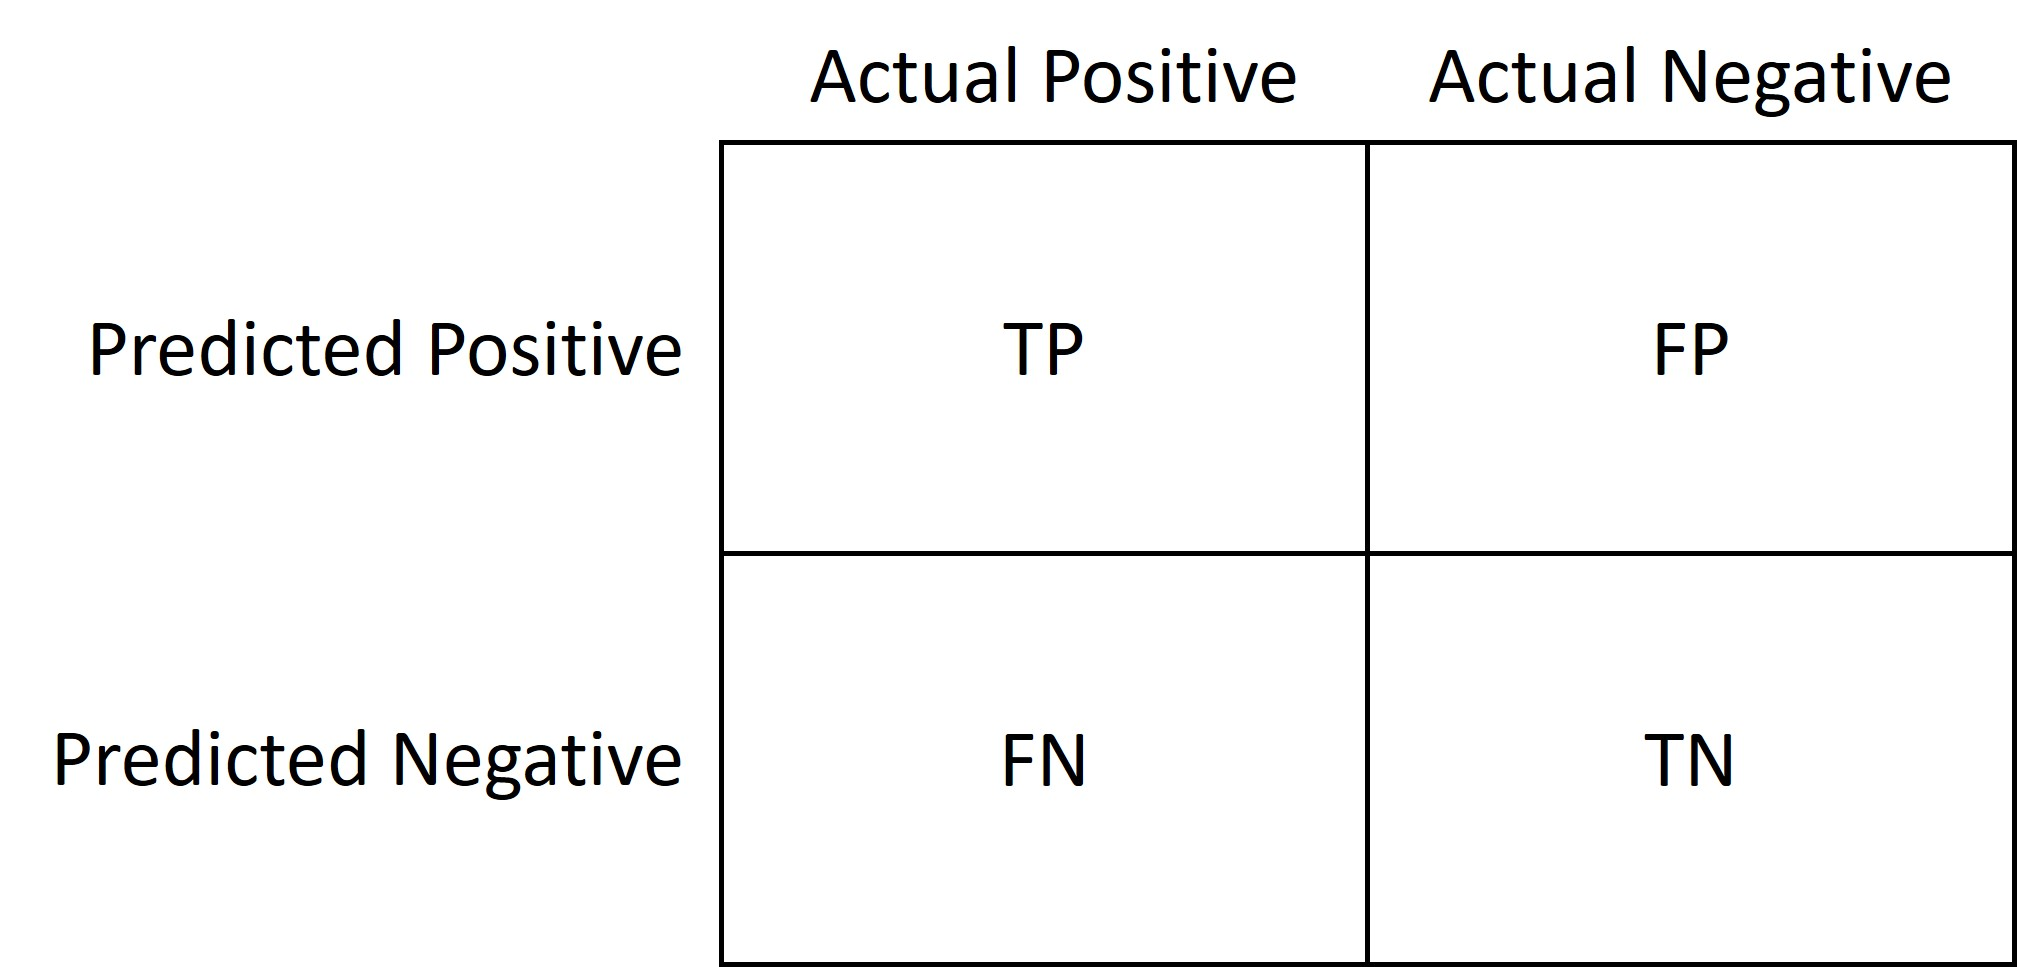
\includegraphics[width=0.75\textwidth]{3/figures/conf_matrix.jpg}
		\caption[Matriz de Confusión]{Matriz de Confusión. \\
		Fuente: Elaboración propia.}
		\label{3:fig302}
	\end{center}
\end{figure}

La matriz consta de cuatro partes importantes: TP, FP, FN y TN. Estos serán usados para presentar las fórmulas de las métricas más adelante. El primero (TP o true positive) se refiere a la cantidad de observaciones que se han predicho como positivos y que en verdad sí son positivos; por el contrario, FP (false positive) se refiere a aquellas predicciones dadas como positivos, pero en verdad son negativos. FN (false negative) es la cantidad de observaciones predichas como negativas; sin embargo, estas en realidad son positivas. Finalmente, TN (true negative) es la cantidad de observaciones predichas como negativas y que en realidad son también negativas.

A continuación, se presenta las métricas para medir el desempeño de la clasificación del modelo.

El accuracy representa aquella proporción del total de predicciones que se ha obtenido correctamente \parencite{ws_izco2018bdcp}. Este se calcula a través de la siguiente fórmula 1.

%\begin{equcaption}[!ht]
\begin{equation}\label{eq:accuracy}
\phantomsection
accuracy=\frac{TP+TN}{TP+TN+FP+FN}
\end{equation}
\myequations{Fórmula para calcular el accuracy}

El recall representa la proporción de solo los positivos reales predichos de manera acertada \parencite{ws_izco2018bdcp}. Se calcula con la siguiente fórmula.

%\begin{equcaption}[!ht]
\begin{equation}\label{eq:recall}
\phantomsection
recall=\frac{TP}{TP+FN}
\end{equation}
\myequations{Fórmula para calcular el recall}

Precision representa aquella proporción de lo predicho positivamente que es positiva \parencite{ws_izco2018bdcp}. Se calcula con la fórmula a continuación.

%\begin{equcaption}[!ht]
\begin{equation}\label{eq:precision}
\phantomsection
precision=\frac{TP}{TP+FP}
\end{equation}
\myequations{Fórmula para calcular el precision}

\begin{landscape}
	\section{Cronograma de actividades y presupuesto}
	Se propuso un cronograma para la investigación. Conforma desde el inicio hasta ser terminada con la sustentación final planeada para mediados del año 2024. Este se presneta en la Figura \ref{3:fig303}.

	\begin{figure}[!ht]
		\begin{center}
			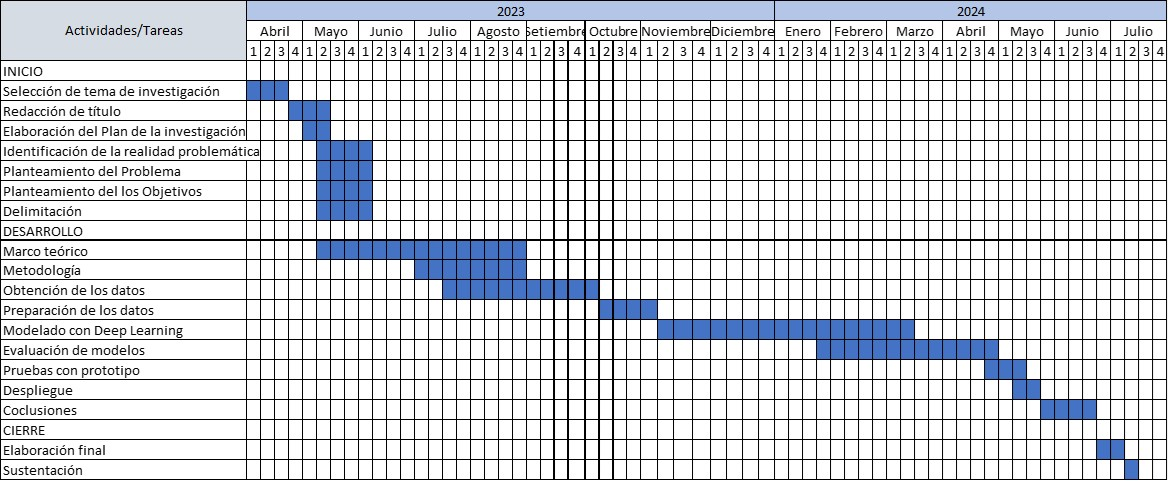
\includegraphics[width=1.50\textwidth]{3/figures/cronograma_tesis_thyr.jpg}
			\caption[Cronograma de actividades]{Cronograma de actividades.\\
				Fuente: Elaboración propia.}
			\label{3:fig303}
		\end{center}
	\end{figure}
	
\end{landscape}

Además, se determinó el presupuesto necesario para la elaboración completa de la investigación. Este se presenta en la Tabla \ref{3:table1}.

\begin{table}[H]
	\caption[Presupuesto]{Presupuesto.}
	\label{3:table1}
	\centering
	\small
	\begin{tabular}{llll}
		\specialrule{.1em}{.05em}{.05em}
		{Grupo} & {Item} & {Costo (soles)} & {Subtotal} \\
		\specialrule{.1em}{.05em}{.05em}
		\multirow{2}{4cm}{Recursos materiales} & {Laptop} & {S/ 6,500.00} & {} \\
		{} & {Materiales de escritorio} & {S/ 100.00} & {S/ 6,600.00} \\
		\cline{1-4}
		\multirow{2}{4cm}{Software y trámites} & {Matrícula de Trabajo de Tesis II} & {S/ 375.00} & {} \\ % & {Reserva de tema} & {S/ 2,700.00} & {} \\
		{} & {Cuotas de Trabajo de Tesis II} & {S/ 1,044.00} & {} \\
		%{} & {Derecho de inscripción} & {S/ 800.00} & {} \\
		%{} & {Derecho de sustentación} & {S/ 1,500.00} & {} \\
		{} & {Software} & {S/ 50.00} & {} \\
		{} & {Renta de servidor en la nube} & {S/ 224.15} & {S/ 1,693.15} \\ % & {S/ 5,274.15} \\
		\cline{1-4}
		\multirow{2}{4cm}{Extras} & {Consultorías} & {S/ 100.00} & {} \\
		{} & {Movilidad} & {S/ 200.00} & {S/ 300.00} \\
		\specialrule{.1em}{.05em}{.05em} 
		{} & {Total} & {} & {S/ 8,593.15} \\ % & {S/ 12,174.15} \\
		\specialrule{.1em}{.05em}{.05em}
	\end{tabular}
	\begin{flushleft}	
		\small Fuente: Elaboración propia.
	\end{flushleft}
\end{table}




%\chapter{Desarrollo de la Solución}
En el presnete capítulo se describe las herramientas y procesos de desarrollo del modelo de Deep Learning.

\section{Determinación y evaluación de alternativas de solución}

En esta sección se presentarán las arquitecturas base CNN y ViT que se usarán en el entrenamiento de los modelos de Deep Learning para la tarea de clasificación de nódulos tiroideos a través de imágenes de ultrasonido. Además, también se introducirá la idea de modelo híbrido que junta las capacidades de extracción de características de los CNN con la actualmente popular arquitectura ViT.

En el grupo de modelos CNN, se tiene en primera instancia a la arquitectura VGG16, ya presentada anteriormente en el Capítulo 2.Este modelo posee 16 capas de profundidad junto con un tamaño de 3 x 3 en los filtros. Se ha reconocido que VGG16, y las arquitecturas VGGNet en general, poseen una alta capacidad de generalización, lo cuál lo vuelve ideal para tareas de clasificación distintas a los que originalmente fue entrenado. \parencite{pr_simonyan2015vdcn}

En segundo lugar, también parte del grupo de modelos CNN, se tiene a ResNet 50, también ya presentado inicialmente en el Capítulo 2. Esta arquitectura introdujo el concepto de redes residuales que permitieron obtener de manera más optimizada un mayor desempeño en arquitecturas de alta profundidad. \parencite{pr_he2016deepres} La versión de ResNet usada en esta investigación fue la de 50 capas de profundidad.

En el conjunto de modelos ViT, el usado en la presente investigación fue la ViT-Base con patch de tamaño 16 x 16.

Los modelos ViT también ya fueron presentados en el Capítulo 2.

Esta arquitectura, basada en los originales Transformers, ha demostrado tener mejor desempeño en tareas de clasificación comparado a los modelos basados en CNNs, aunque ciertamente con una mayor necesidad de datos de entrenamiento.

En la Figura \ref{2:fig206}, ya se muestra la forma de la arquitectura del modelo ViT. Cabe volver a resaltar que la versión del modelo ViT utilizado es el Base que consta de 86 millones de parámetros y recibe patch de tamaño 16 x 16.

Finalmente, el último modelo presente en la investigación es uno que combina la capacidad de los CNN y los ViT para obtener un modelo híbrido.

Este modelo utiliza al CNN como backbone que alimentará los features extraídos en forma de patch de tamaño 1 x 1 al modelo ViT. Para lograr esto se es necesario quitar el cabezal clasificador de la arquitectura CNN, pues esta tarea ya será desarrollada por el propio ViT.

Debido a las limitaciones de tiempo y recursos, solamente se desarrollará dos modelos híbridos con aquellos CNN de mejor desempeño en los entrenamientos iniciales.

Cabe destacar que este modelo híbrido fue inspirado por el trabajo presentado por \cite{pr_JERBI2023autoclassViTGAN}. A continuación se presenta la Figura \ref{4:fig101}, donde se muestra la arquitectura híbrida.

\begin{figure}[H]
	\begin{center}
		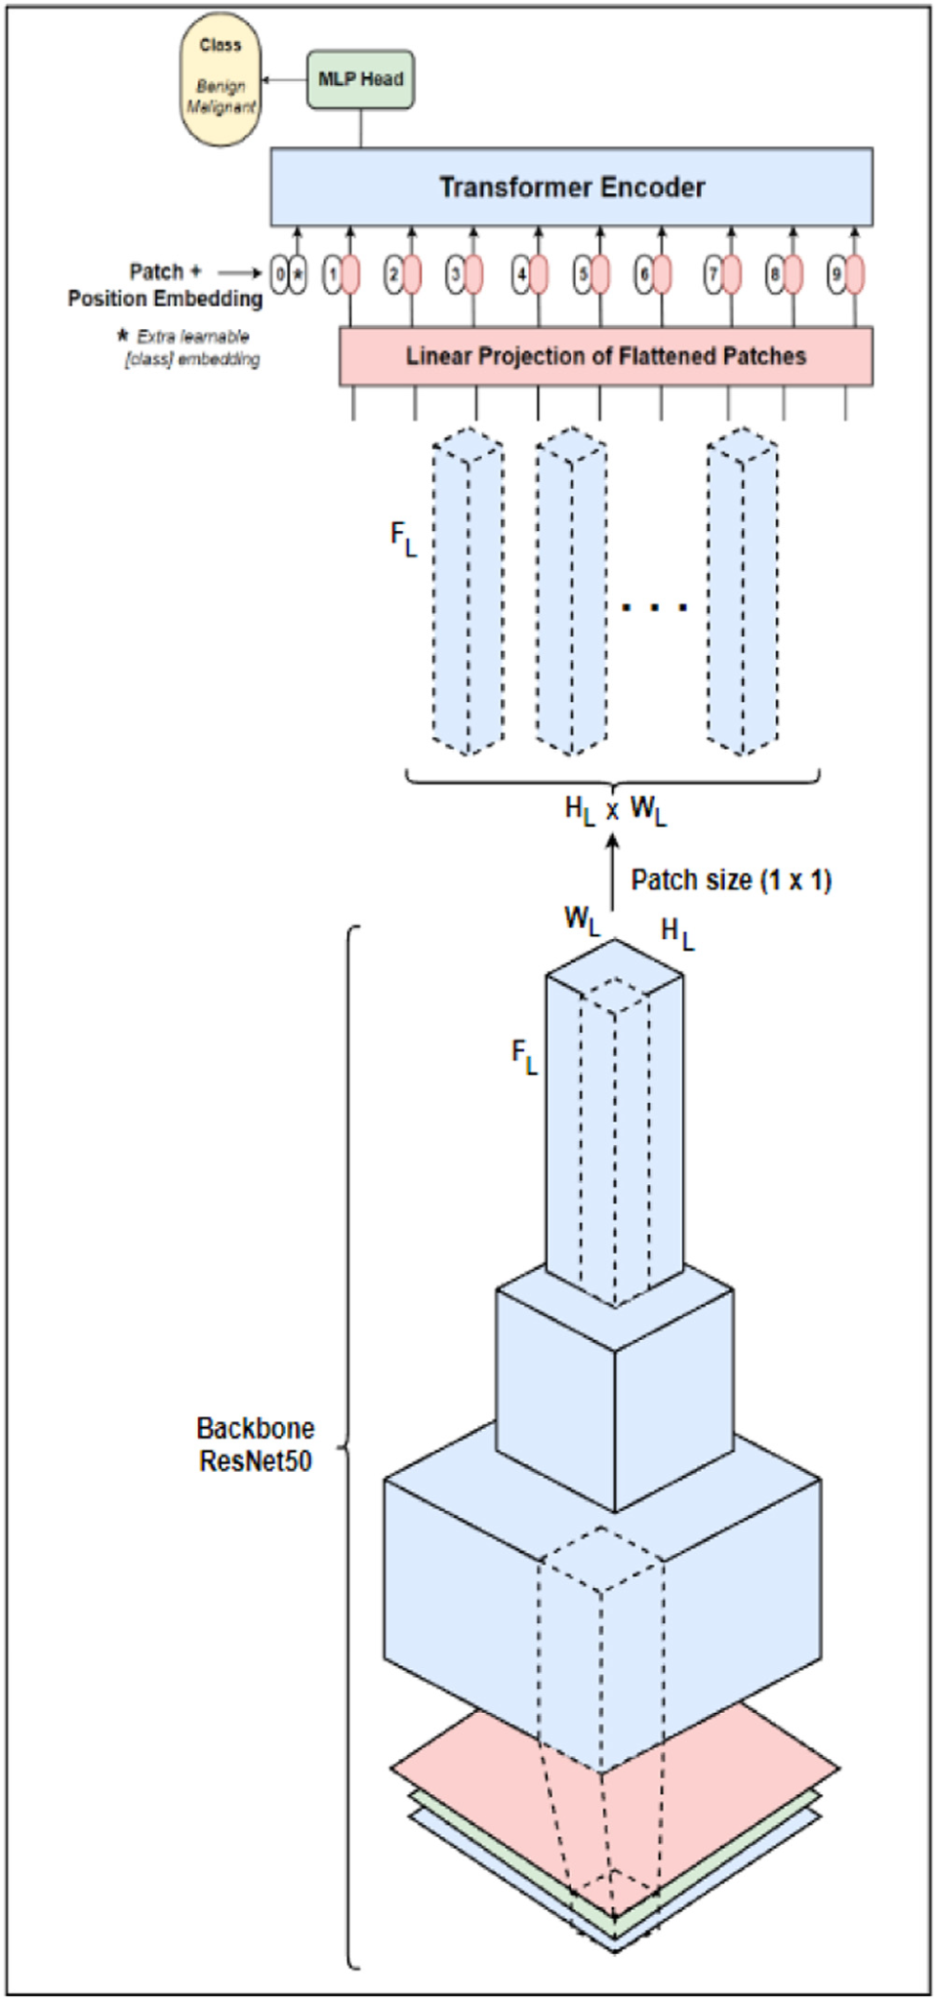
\includegraphics[width=0.60\textwidth]{4/figures/hybrid_arc.png}
		\caption[Imágenes de ultrasonido de la tiroides generadas]{Imágenes de ultrasonido de la tiroides generadas. \\
		Fuente: \cite{pr_JERBI2023autoclassViTGAN}. \textit{Automatic classification of ultrasound thyroids images using vision transformers and generative adversarial networks}.}
		\label{4:fig101}
	\end{center}
\end{figure}

\section{Propuesta solución}

\subsection{Planeamiento y descripción de Actividades}

La metodología descrita en el capítulo anterior consta de tres etapas principales: adquisición de datos, preprocesamiento de los datos y la aplicación de Deep Learning; es decir, el entrenamiento de los diferentes tipos de algoritmos. En la siguiente parte de esta investigación se procederá describir las actividades necesarias para desarrollar y completar cada una de estas etapas para, finalmente, obtener los resultados de cada uno de los modelos entrenados.

La metodología inicia con la adquisición del conjunto de datos necesario para realizar el entrenamiento de los modelos de Deep Learning. Este consta de las siguientes actividades.

\textbf{Actividad 1: Buscar y revisar bases de datos sobre imágenes de ultrasonido de nódulos tiroideos}
\\
En esta actividad se investigarán y analizarán aquellos conjunto de datos que cumplan con las características básicas requeridas: poseer imágenes de ultrasonido de nódulos tiroideos benignos y malignos.

\textbf{Entregable:} Diversos conjuntos de datos de imágenes de ultrasonido de nódulos tiroideos benignos y malignos.
\\

\textbf{Actividad 2: Filtrado de los conjuntos de datos}
\\
El conjunto de datos seleccionado debe cumplir con los siguientes requerimientos: las imágenes deben poseer información del carácter del nódulo; en otras palabras, se debe tener información sobre la imagen cada imagen de ultrasonido donde se indique si se está ante un nódulo de carácter benigno o maligno. Otra importante característica, necesaria para evitar obtener completamente distintos resultados en futuras investigaciones, es la fuente de origen de las imágenes del conjunto de datos, ya que este debe poseer imágenes de diferentes instituciones y herramientas. Esta característica permitirá a los modelos a entrenar tener la capacidad de afrontar distintas calidades y tipos de imágenes de ultrasonido. La última característica radica en la cantidad de las imágenes, ya que el conjunto de datos debe poseer una moderada cantidad de datos que permitan a los modelos interpretar mejor las imágenes de ultrasonido, y así finalmente aumentar la capacidad de generalización del modelo.

\textbf{Entregable:} Conjunto de datos de imágenes de ultrasonido de nódulos tiroideos benignos y malignos que cumple con todas las características requeridas.
\\
En la etapa de preprocesamiento, necesaria para realizar un correcto entrenamiento de los modelos de Deep Learning, se realizará un análisis y limpieza de los datos, además, se pasará por un proceso de preparamiento de los datos para facilitar el flujo de los datos a través de los de los modelos a entrenar. Esta etapa consta de dos flujos, donde uno de estos incluye el Aumento de Datos con el modelo DCGAN; mientras que el otro, evita el paso por este proceso debido a la fiabilidad de este tipo de red para generar datos que puedan ser útiles para el entrenamiento de los modelos. Ambos flujos constan de las tres primeras actividades descritas a continuación.

\textbf{Actividad 1: Explorar características del conjunto de datos}
\\
Se inicia con la exploración del conjunto de datos seleccionado, extrayendo gráficas y tablas que muestren su composición y características, permitiendo así determinar qué técnicas se podrían aplicar para mejorar las flaquezas del conjunto de datos. Aquí se puede obtener información sobre la necesidad o no de aplicar el Aumento de Datos a una clase minoritaria si lo hubiera.

\textbf{Entregable:} Gráficas y tablas de características y composición del conjunto de datos.
\\

\textbf{Actividad 2: Filtrar y organizar imágenes poco útiles del conjunto de datos}
\\
Se realizará un filtrado de aquellas imágenes corruptas, atípicas o sin etiqueta, dejando solo en el conjunto de datos a aquellas de mayor utilidad, al mismo tiempo que se reorganiza en un nuevo formato de ficheros para facilitar su posterior carga a los modelos de Deep Learning.

\textbf{Entregable:} Conjunto de datos organizados y sin imágenes corruptas, atípicas o sin etiquetas.
\\

\textbf{Actividad 3: Redimensionar, normalizar y dividir los datos según los requerimientos para cada modelo de Deep Learning}
\\
Inicialmente se aplicará a cada imagen un redimensionamiento y normalización según se vea conveniente, esto con el fin de evitar mayor complejidad computacional y reducir los tiempos de ejecución de los modelos. Luego se hará una división del conjunto de datos total en data de entrenamiento, validación y prueba.

\textbf{Entregable:} Conjunto de datos de entrenamiento, validación y prueba preprocesados.
\\
El segundo flujo de la metodología, al evitar el proceso de Aumento de Datos, obvia la siguiente actividad y continúa directamente en la siguiente etapa.

\textbf{Actividad 4: Mejorar composición del conjunto de datos}
\\
El Aumento de Datos se debe utilizar en caso de desbalance de clases en el conjunto de datos con el objetivo de aumentar la capacidad de generalización del modelo y evitar su sobreajuste.

Debido a las características que determinan si una imagen de ultrasonido es benigno o maligno (forma, orientación, tamaño y nivel de brillo), usar las técnicas comunes de Aumento de Datos de hacer diferentes transformaciones en las imágenes originales de forma aleatorio, no tendría sentido. Por este motivo, en esta actividad, se entrenará un modelo DCGAN personalizado que logre aprender la distribución de las imágenes reales y pueda generar posteriormente imágenes sintéticas. El entrenamiento de este modelo se realizará a través del conjunto de datos de entrenamiento obtenido de la anterior actividad, seleccionando aquellos pertenecientes a la clase de minoritaria.

Ya con el modelo entrenado, este será utilizado para generar y aumentar la cantidad de datos final para la clase minoritaria en la data de entrenamiento.

\textbf{Entregable:} Conjunto de datos con ambas clases balanceadas.
\\
Una vez se termina el preprocesamiento y se obtiene la data final, se continúa con el entrenamiento y validación de modelos de Deep Learning, seguido de una prueba final con la data respectiva. Esta etapa se divide en las siguientes actividades.

\textbf{Actividad 1: Seleccionar algoritmos a entrenar según usos y resultados de las investigaciones presentadas en los antecedentes}
\\
Se revisará aquellas arquitecturas utilizadas en las investigación mencionadas en el Capítulo 2. De todas las recolectadas, se seleccionarán las de mejor desempeño y de mayor presencia.

\textbf{Entregable:} Arquitecturas de Deep Learning ideales para la tarea de clasificación de imágenes de ultrasonido de nódulos tiroideos.
\\

\textbf{Actividad 2: Entrenar y probar los modelos de Deep Learning previamente definidos}
\\
Se realizará el entrenamiento de cada uno de las diferentes arquitecturas con configuraciones establecidas por anteriores investigaciones. También se aplicarán dos técnicas por separado para este proceso: Transfer Learning y Fine Tuning. Además, en cada época de entrenamiento de todos los modelos, se usará el conjunto de datos de validación para verificar el avance de la capacidad predictiva de los modelos.

Finalmente, cada uno de estos modelo será puesto a prueba en el conjunto de datos restantes (data de prueba), así finalmente se obtendrán las métricas correspondientes que permitirán luego realizar el análisis de desempeño.

\textbf{Entregable:} Modelos CNN y ViT entrenados. Métricas de cada uno de los modelos.
\\

\textbf{Actividad 3:  Definir modelos híbridos entre ViT y CNN}
\\
Se desarrollarán modelos híbridos entre CNN y ViT. En cada uno de estos, la arquitectura CNN funcionará como backbone o modelo base que recibirá las imágenes y posteriormente alimentará al modelo ViT.

Debido a la limitación de tiempo y poder computacional al que se puede acceder, solamente se seleccionará dos modelo CNN de mejor desempeño como backbone para elaborar dos híbridos. Adicionalmente, también se utilizará un modelo híbrido totalmente preentrenado.

\textbf{Entregable:} Modelos híbridos CNN + ViT.
\\

\textbf{Actividad 4: Entrenar y probar modelos híbridos CNN + ViT}
\\
Al igual que los anteriores modelos, estos nuevos modelos híbridos serán entrenados con la misma data de entrenamiento y con las mismas configuraciones, a excepción de algunas variaciones.

En este caso solo se aplicará la técnica de Fine Tuning debido a la capacidad de procesamiento disponible.

En cada época del entrenamiento, se usará la data de validación para verificar su desempeño en este proceso.

Finalmente, al igual que los otros modelos, los híbridos también serán sometidos al conjunto de datos de prueba para obtener sus métricas correspondientes.

\textbf{Entregable:} Modelos híbridos CNN + ViT entrenandos. Métricas de los modelos híbridos.
\\

\subsection{Desarrollo de actividades}

En esta sección de la investigación se procederá a desarrollar cada una de las actividades aplicando las técnicas y herramientas ya mencionadas en anteriores capítulos siguiendo la metodología de implementación previamente definida.

La primera etapa de Adquisición del conjunto de datos se desarrollaron las ya definidas actividades de la siguiente forma.

\textbf{Actividad 1: Buscar y revisar bases de datos sobre imágenes de ultrasonido de nódulos tiroideos}
\\
En los antecedentes presentados en la sección 2.1, la mayoría de investigaciones relacionadas a imágenes de ultrasonido de nódulos tiroideos, no posee datos de acceso libre, esto conlleva a que se tenga una limitada cantidad de opciones de donde escoger y filtrar el conjunto de datos a usar para entrenar y probar los modelos de Deep Learning.

La base de datos más popular y de acceso libre de imágenes de ultrasonido de nódulos tiroides es el dado por la Universidad de Colombia, CIM@LAB y IDIME (Instituto de Diagnóstico Médico). Este conjunto de datos consta de 472 imágenes, de las cuales, la amplia mayoría (397) son de nódulos malignos, mientras que los restantes pertenecen a aquellos de carácter benigno. Este conjunto de datos posee, además, anotaciones de expertos en archivos de formato XML, donde indica diversas características de las imágenes, además de datos personales de los pacientes. En la Figura \ref{4:fig102} se muestra algunas imágenes de este conjunto de datos, mientras que en la Figura \ref{4:fig103} se muestra un ejemplo de archivo XML también presente.

\begin{figure}[H]
	\begin{center}
		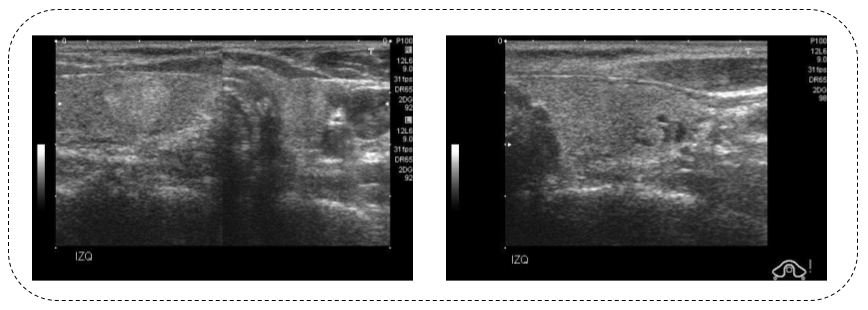
\includegraphics[width=0.85\textwidth]{4/figures/nodule_ddti.png}
		\caption[Ejemplo de imágenes del conjunto de datos de la Universidad de Colombia]{Ejemplo de imágenes del conjunto de datos de la Universidad de Colombia. \\
		Fuente: Elaboración propia.}
		\label{4:fig102}
	\end{center}
\end{figure}

\begin{figure}[H]
	\begin{center}
		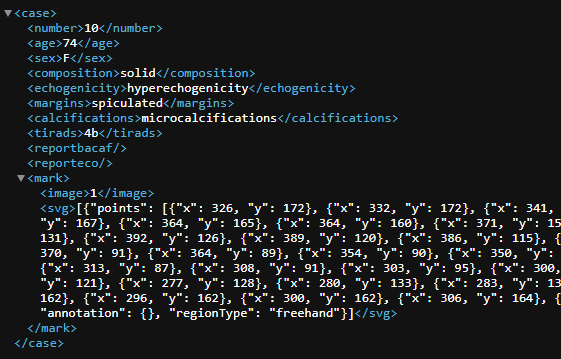
\includegraphics[width=0.65\textwidth]{4/figures/xmlfile.png}
		\caption[Ejemplo de archivo XML del conjunto de datos de la Universidad de Colombia]{Ejemplo de archivo XML del conjunto de datos de la Universidad de Colombia. \\
		Fuente: Elaboración propia.}
		\label{4:fig103}
	\end{center}
\end{figure}

Otro conjunto de datos, también de acceso libre, aunque no tan difundido como el presentado anteriormente es el otorgado por Zhujiang Hospital of Southem Medical University que recopila imágenes de 2421 pacientes obteniendo un total de 3493 imágenes de ultrasonido, de los cuales, 2283 pertenecen a imágenes de glándulas de tiroides con nódulos de carácter benigno, mientras que 1210 pertenecen a nódulos malignos. Además, este conjunto de datos también posee archivos CSV donde especifica el nombre de la imagen y la etiqueta a la que pertenece: benigno (0) o maligno (1).

Cabe destacar que este conjunto de datos posee características particulares que lo diferencian del primero, y es que este, además de estar validado por distintos comités de ética en China, procede de distintas fuentes; es decir, las imágenes pueden variar de tamaño y/o calidad entre sí.

En la Figura \ref{4:fig104} se muestran algunas imágenes de este conjunto de datos, mientras que en la Figura \ref{4:fig105} se muestra una sección de los archivos CSV.

\begin{figure}[H]
	\begin{center}
		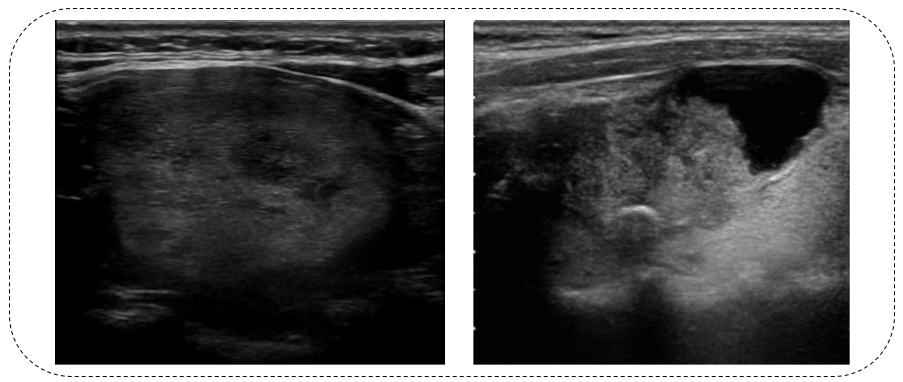
\includegraphics[width=0.68\textwidth]{4/figures/tn3k_examp.png}
		\caption[Ejemplo de imágenes del conjunto de datos de Zhujiang Hospital of Southem Medical University]{Ejemplo de imágenes del conjunto de datos de Zhujiang Hospital of Southem Medical University. \\
		Fuente: Elaboración propia.}
		\label{4:fig104}
	\end{center}
\end{figure}

\begin{figure}[H]
	\begin{center}
		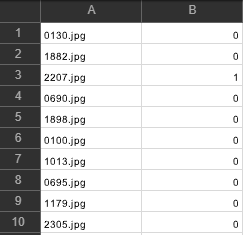
\includegraphics[width=0.38\textwidth]{4/figures/tn3k_csv.PNG}
		\caption[Ejemplo de archivo CSV del conjunto de datos de Zhujiang Hospital of Southem Medical University]{Ejemplo de archivo CSV del conjunto de datos de Zhujiang Hospital of Southem Medical University. \\
		Fuente: Elaboración propia.}
		\label{4:fig105}
	\end{center}
\end{figure}

\textbf{Actividad 2: Filtrado de los conjuntos de datos}
\\
Los requerimientos para un buen conjunto de datos radica principalmente en la información del tipo o carácter del nódulo, el origen de las imágenes de ultrasonido y la cantidad de datos.

El conjunto de datos otorgado por la Universidad de Colombia, CIM@LAB y IDIME poseía buena información, superando el requerimiento base de tipo o carácter del nódulo, pues otorgaba datos del paciente que podrían ser útiles a la hora de realizar el proceso de prediagnóstico; sin embargo, la gran debilidad del este conjunto de datos es la poca cantidad de imágenes que posee. Además, el hecho de no definirse el origen específico de estas imágenes en relación a si se obtuvo de distintas instituciones con diferentes herramientas o no, conllevó finalmente a su descarte.

El conjunto de datos de Zhujiang Hospital of Southem Medical University cumple exactamente con otorgar información sobre el carácter de los nódulos de cada imagen que posee, además, también se especifica el origen variado de las imágenes, pues fueron recopiladas de distintas instituciones y con diferentes herramientas. Finalmente, la cantidad de datos, aunque con clases desbalanceadas, supera en gran medida al primer conjunto de datos.

Al cumplir con todos los requerimientos para el entrenamiento de un buen modelo Deep Learning, el conjunto de datos finalmente seleccionado fue el de Zhujiang Hospital of Southem Medical University.

Como se mencionó en la sección anterior, la etapa siguiente es la de preprocesamiento. En este se realizó un completo análisis, limpieza y preparación de los datos para el entrenamiento de los modelos.

Cabe recordar además la existencia de dos flujos en este proceso igualmente descritos en la sección anterior. Ambos inician de igual forma con las tres siguientes actividades.

\textbf{Actividad 1: Explorar características del conjunto de datos}
\\
Ya con el conjunto de datos seleccionado, se utilizó la data almacenada en los archivos CSV (mostrado en la Figura \ref{4:fig105}) para contabilizar la cantidad de imágenes por cada clase y así determinar si existía o no la presencia de desbalance. La Figura \ref{4:fig106} y Figura \ref{4:fig107} muestran gráficas circulares donde se aprecia la proporción del total de datos por cada clase y por cada tipo de datos (entrenamiento y prueba).

\begin{figure}[H]
	\begin{center}
		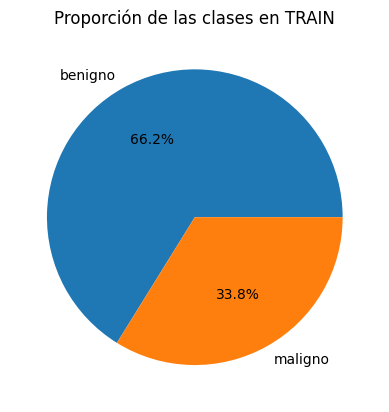
\includegraphics[width=0.51\textwidth]{4/figures/train_circular.png}
		\caption[Gráfica circular de conjunto de datos de entrenamiento]{Gráfica circular de conjunto de datos de entrenamiento. \\
		Fuente: Elaboración propia.}
		\label{4:fig106}
	\end{center}
\end{figure}

\begin{figure}[H]
	\begin{center}
		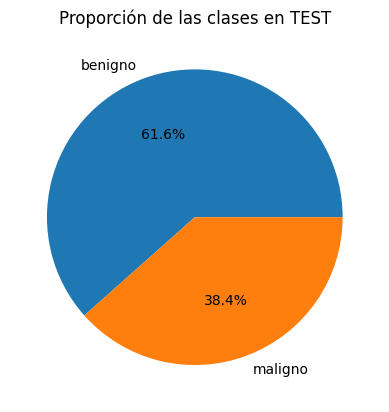
\includegraphics[width=0.51\textwidth]{4/figures/test_circular.png}
		\caption[Gráfica circular de conjunto de datos de prueba]{Gráfica circular de conjunto de datos de prueba. \\
		Fuente: Elaboración propia.}
		\label{4:fig107}
	\end{center}
\end{figure}

En ambas figuras se puede verificar la presencia de desbalance en clases, observando además como la clase de nódulos benignos duplica aproximadamente a la cantidad de imágenes de la clase de nódulos malignos. Este comportamiento se ve reflejado tanto para los datos de entrenamiento como para los de prueba.

Este descubrimiento afirmó la necesidad de aplicar una técnica de balanceo de datos.

\textbf{Actividad 2: Filtrar y organizar imágenes poco útiles del conjunto de datos}
\\
A través del Algoritmo \ref{4:alg101} se logró filtrar y obviar aquellas imágenes corruptas (en el caso de este conjunto de datos no se tuvo ninguno). Además, este también permitió la lectura de solo las imágenes con nombre presente en los archivos CSV, lo cual logró evitar el cargado de imágenes sin etiqueta alguna (en el caso de este conjunto de datos tampoco se tuvieron imágenes sin etiquetas). Finalmente, todas aquellos datos que cumplieran con los anteriores pasos serían trasladados a la nueva distribución de ficheros mostrada en la Figura \ref{4:fig109}.
%\hspace{\algorithmicindent} 
\begin{algorithm}[H]
	\caption{Proceso de organización y traslado de imágenes}
	\label{4:alg101}
	\begin{algorithmic}[1]
		\State \textbf{Entradas:} $pd\_train$, $pd\_test$, $source\_dir\_train$, $source\_dir\_test$, $train\_dir$, $test\_dir$
		\State Obtener nombres de imágenes de entrenamiento de $pd\_train$
		\State Crear diccionario $d$ de nombres a etiquetas de $pd\_train$
		\For{cada nombre de imagen $im$ en nombres de imágenes de entrenamiento}
			\State \textbf{Intentar:}
			\If{etiqueta de $im$ en $d$ es 1}
				\State Copiar $im$ a $train\_dir/malignant$
			\ElsIf{etiqueta de $im$ en $d$ es 0}
				\State Copiar $im$ a $train\_dir/benign$
			\EndIf
			\State \textbf{Excepción:}
			\State \textbf{Imprimir:} La imagen $im$ no se ha podido cargar...
		\EndFor

		\State Obtener nombres de imágenes de prueba de $pd\_test$
		\State Crear diccionario $dt$ de nombres a etiquetas de $pd\_test$
		\For{cada nombre de imagen $im$ en nombres de imágenes de prueba}
			\State \textbf{Intentar:}
			\If{etiqueta de $im$ en $dt$ es 1}
				\State Copiar $im$ a $test\_dir/malignant$
			\ElsIf{etiqueta de $im$ en $dt$ es 0}
				\State Copiar $im$ a $test\_dir/benign$
			\EndIf
			\State \textbf{Excepción:}
			\State \textbf{Imprimir:} La imagen $im$ no se ha podido cargar...
		\EndFor

		\State \textbf{Imprimir:} SE TRASLADARON TODAS LAS IMÁGENES AL NUEVO DIRECTORIO!
	\end{algorithmic}
\end{algorithm}

\begin{comment}
	\begin{figure}[H]
		\begin{center}
			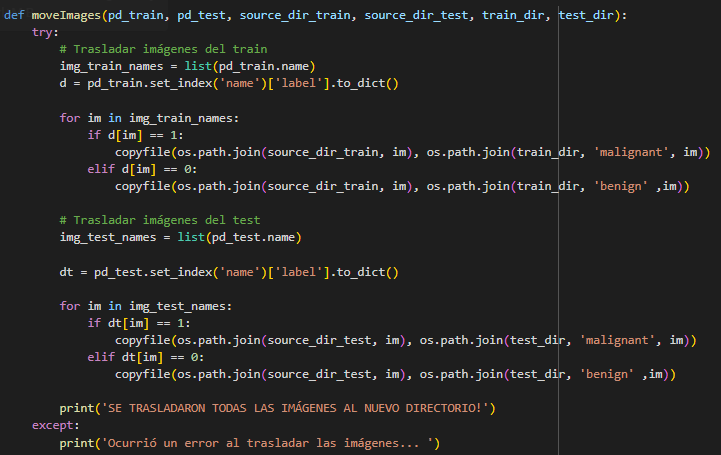
\includegraphics[width=0.75\textwidth]{4/figures/algoritm_organi.PNG}
			\caption[Algoritmo de organización de imágenes]{Algoritmo de organización de imágenes. \\
			Fuente: Elaboración propia.}
			\label{4:fig108}
		\end{center}
	\end{figure}
	
\end{comment}

\begin{figure}[H]
	\begin{center}
		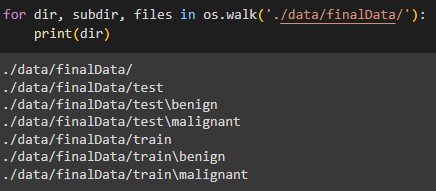
\includegraphics[width=0.60\textwidth]{4/figures/nuevos_ficheros.PNG}
		\caption[Nueva distribución de ficheros para los datos]{Nueva distribución de ficheros para los datos. \\
		Fuente: Elaboración propia.}
		\label{4:fig109}
	\end{center}
\end{figure}

\textbf{Actividad 3: Redimensionar, normalizar y dividir los datos según los requerimientos para cada modelo de Deep Learning}
\\
A partir de esta actividad, los datos usados fueron aquellos anteriormente trasladados desde los ficheros originales a los nuevos directorios.

El tamaño a redimensionar de las imágenes del conjunto de datos dependió únicamente del modelo en el que este se usó.

La normalización de los valores de píxeles de cada imagen se hizo con un media y desviación estándar de 0.5 aplicadas a cada uno de los 3 canales de las imágenes. Esto llevó a obtener finalmente píxeles con valores dentro del rango de [-1, 1], lo cual se recomienda para realizar entrenamientos de los modelos de forma más eficiente.

Finalmente, el conjunto de datos de entrenamiento se dividió en dos partes: data de validación, el cual representa el 15\% del total, y data de entrenamiento, compuesta del 85\% restante. La distribución de los datos se hizo de forma aleatoria manteniendo los mismos porcentajes.

La cantidad de la data de prueba se mantuvo igual a como originalmente fue obtenida.

Todo este proceso se realizó a través del Algoritmo \ref{4:alg102}, donde finalmente se otorgaron los tres conjuntos de datos en tipo DataLoader de Pytorch que posteriormente facilitó la ingesta de datos a los modelos.

\begin{algorithm}[H]
	\caption{Preparación de datos para entrenamiento, validación y prueba}
	\label{4:alg102}
	\begin{algorithmic}[1]
		\State \textbf{Entradas:} $train\_dir$, $test\_dir$, $img\_size$, $b\_size$
		\State \textbf{Salidas:} $train\_gen$, $val\_gen$, $test\_gen$
		
		\Procedure{DefinirTransformaciones}{}
			\State Redimensionar imágenes a $img\_size$
			\State Recortar las imágenes a $img\_size$
			\State Convertir imágenes a tensores
			\State Normalizar tensores con medias y desviaciones estándar $(0.5, 0.5, 0.5)$
		\EndProcedure
		
		\Procedure{CargarDatos}{}
			\State Cargar imágenes de entrenamiento de $train\_dir$ con transformaciones
			\State Cargar imágenes de prueba de $test\_dir$ con transformaciones
		\EndProcedure
		
		\Procedure{DividirDatosEntrenamiento}{}
			\State Calcular $val\_size$ como $15\%$ de $train\_data$
			\State Calcular $train\_size$ como $len(train\_data) - val\_size$
			\State Dividir de forma aleatoria $train\_data$ en $train\_data$ y $val\_data$ usando $train\_size$ y $val\_size$
		\EndProcedure
		
		\Procedure{CrearDataloaders}{}
			\State Crear $train\_gen$ para $train\_data$ con $b\_size$
			\State Crear $val\_gen$ para $val\_data$ con $b\_size$
			\State Crear $test\_gen$ para $test\_data$ con $b\_size$
		\EndProcedure
		
		\State \Return $train\_gen$, $val\_gen$, $test\_gen$
	\end{algorithmic}
\end{algorithm}

\begin{comment}
	\begin{figure}[H]
		\begin{center}
			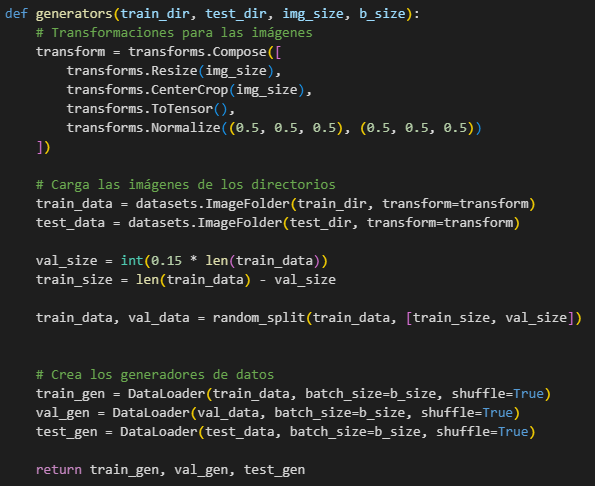
\includegraphics[width=0.70\textwidth]{4/figures/algoritm_dataloader.PNG}
			\caption[Algoritmo para lectura de los datos en DataLoader]{Algoritmo para lectura de los datos en DataLoader. \\
			Fuente: Elaboración propia.}
			\label{4:fig110}
		\end{center}
	\end{figure}
\end{comment}

\textbf{Actividad 4: Mejorar composición del conjunto de datos}
\\
Como se ha mencionado en la sección anterior de este capítulo, las características que determinan si un nódulo puede ser benigno o maligno en un imagen de ultrasonido impiden el uso de las técnicas convencionales de Aumento de Datos. Por este motivo, se construyó un modelo DCGAN con el objetivo de generar imágenes sintéticas.

Inicialmente, la arquitectura del modelo DCGAN siguió los mismos lineamientos definidos en la página oficial de Pytorch por \cite{ws_inkawhich2024dcganpytorch}; sin embargo, debido a la posible pérdida de información al reducir considerablemente el tamaño de las imágenes (ya que se pedía como entrada imágenes de 64 x 64), se decidió por personalizar el modelo original para que pueda recibir imágenes de 128 x 128, de la misma manera como se hizo en la investigación presentada por \cite{pr_JERBI2023autoclassViTGAN}. Para lograr esto se tuvo que modificar tanto la red generadora como la discriminadora.

En la red generadora se agregaron un bloque nuevo de capas similar a las que ya poseída, modificando únicamente el tamaño de canales de salida de la capa ConvTranspose2d al doble de las que poseía la capa inicial original. El tamaño de kernel, stride y padding de esta misma capa se mantuvieron del formato original. En la capa de BatchNorm2d también se duplicó la cantidad de features que recibía. La función de activación ReLU se mantuvo con la misma configuración inicial. La capas siguientes a este nuevo bloque, fueron adaptándose a la cambiada cantidad de canales de salida.

El tamaño del vector latente que ingresa a la red generadora se definió en 200, con 3 como número de canales y 128 como cantidad base de features map.

En el caso de la red discriminadora, se introdujo un bloque intermedio de capas en la parte final de todo el grupo de bloque de capas similares. La capa Conv2d de este nuevo bloque recibiría la cantidad de canales de salida del bloque anterior, mientras que sus canales de salida serían el doble de los tenía la capa Conv2d anterior. De igual forma, la capa BatchNorm2d  duplicó la cantidad de features que recibía originalmente. Se mantuvo la misma configuración de la función de activación LeakyReLU. La capa siguiente a este bloque recién creado se modificó para recibir el doble de canales de los que recibía originalmente.

La cantidad de canales que recibía el modelo se estableció en 3, mientras que el número de features map base a generar se estableció a 32.

Todas las demás configuraciones en ambas redes se dejaron por defecto.

La Figura \ref{4:fig111} muestra la arquitectura final de la red generadora.

\begin{figure}[H]
	\begin{center}
		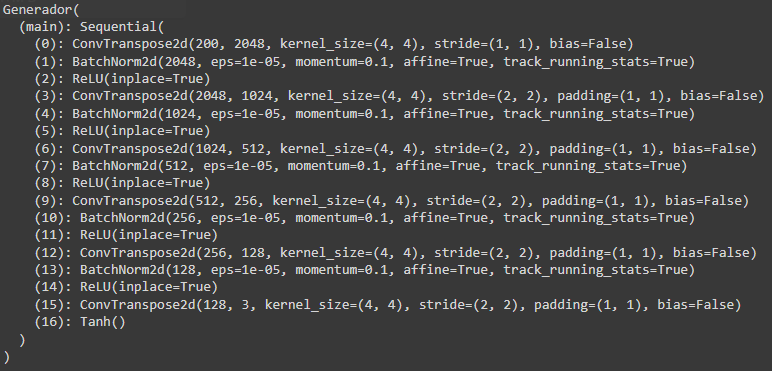
\includegraphics[width=0.78\textwidth]{4/figures/generator_network.PNG}
		\caption[Arquitectura de Red Generadora]{Arquitectura de Red Generadora. \\
		Fuente: Elaboración propia.}
		\label{4:fig111}
	\end{center}
\end{figure}

De igual forma, la Figura \ref{4:fig112}, muestra la arquitectura de la red discriminadora. 

\begin{figure}[H]
	\begin{center}
		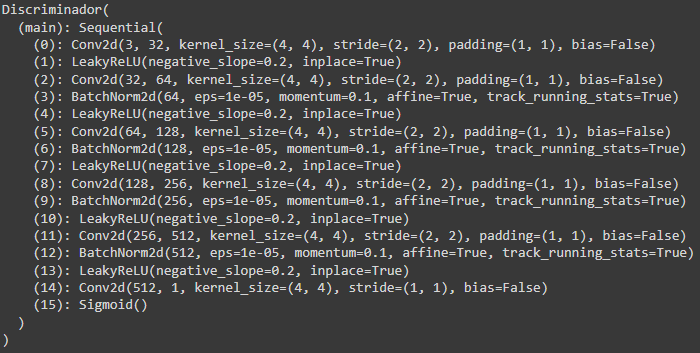
\includegraphics[width=0.76\textwidth]{4/figures/discriminator_network.PNG}
		\caption[Arquitectura de Red Discriminadora]{Arquitectura de Red Discriminadora. \\
		Fuente: Elaboración propia.}
		\label{4:fig112}
	\end{center}
\end{figure}

Para la función de pérdida se usó el Binary Cross Entropy Loss, mientras que la función de optimización se estableció en Adam con una tasa de aprendizaje de 0.0002 y betas de 0.5 para el primero y 0.999 para el segundo. Todo esto según lo establecido por la página oficial de Pytorch.

También se definió un tensor fijo de tamaño 200 (tamaño anteriormente definido de vector latente) inicializado con números aleatorios pero que siguen una distribución normal. Este tensor tenía un lote de tamaño 64.

Para ya iniciar con el entrenamiento del modelo DCGAN se procedió con la creación del DataLoader de Pytorch que contenía todas las imágenes del conjunto de datos de entrenamiento. En este proceso, se definió que las imágenes deberían ser redimensionadas a tamaño 128 y con leídas en un tamaño de lote 64.

El proceso de entrenamiento siguió las características normales del DCGAN original, estableciendo únicamente la cantidad de épocas a 200.

Se usó las capacidades de la GPU NVIDIA A100-SXM4-40GB obtenido a través de Google Colab para este proceso de entrenamiento.

En la Figura \ref{4:fig113} se muestran las métricas de la parte final del entrenamiento.

\begin{figure}[H]
	\begin{center}
		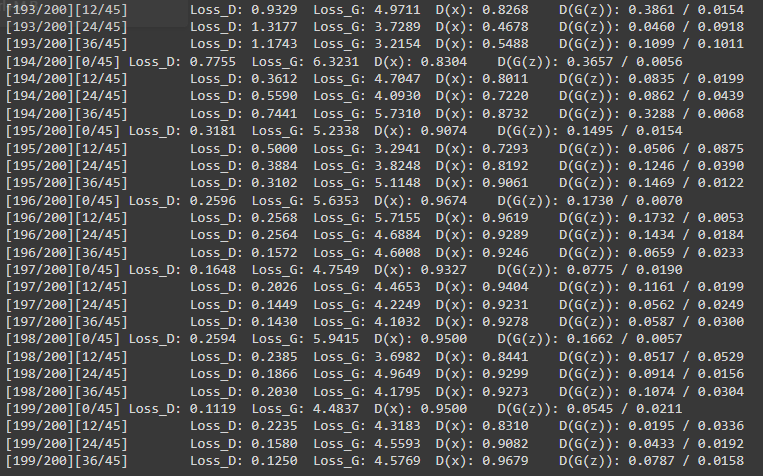
\includegraphics[width=0.75\textwidth]{4/figures/dcgan_1_train.PNG}
		\caption[Parte final del entrenamietno del DCGAN]{Parte final del entrenamietno del DCGAN. \\
		Fuente: Elaboración propia.}
		\label{4:fig113}
	\end{center}
\end{figure}

Además, se realizó un plot de las pérdidas de ambas redes a través de cada iteración del entrenamiento del modelo. Este se muestra en la Figura \ref{4:fig114}.

\begin{figure}[H]
	\begin{center}
		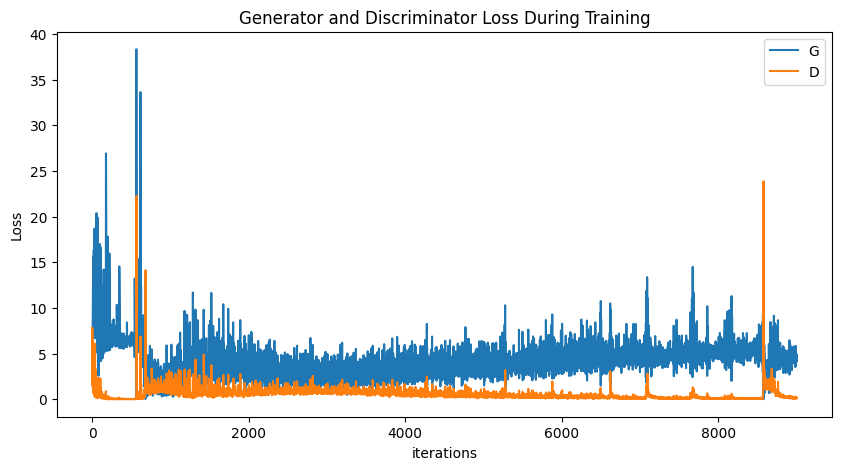
\includegraphics[width=0.85\textwidth]{4/figures/plot_loss_1.png}
		\caption[Plot de pérdidas de las red Generadora y Discriminadora]{Plot de pérdidas de las red Generadora y Discriminadora. \\
		Fuente: Elaboración propia.}
		\label{4:fig114}
	\end{center}
\end{figure}

En esta última gráfica se puede observar cómo ambas pérdidas van convergiendo a más iteraciones se tiene; sin embargo, ya en la parte final se logra observar la divergencia de ambos valores. Esto podría deberse a un sobreajuste por parte de la red discriminadora, al mismo tiempo que la red generadora deja de mejorar en la tarea de generar imágenes sintéticas.

Las imágenes reales y generadas se muestran en la Figura \ref{4:fig115}.

\begin{figure}[H]
	\begin{center}
		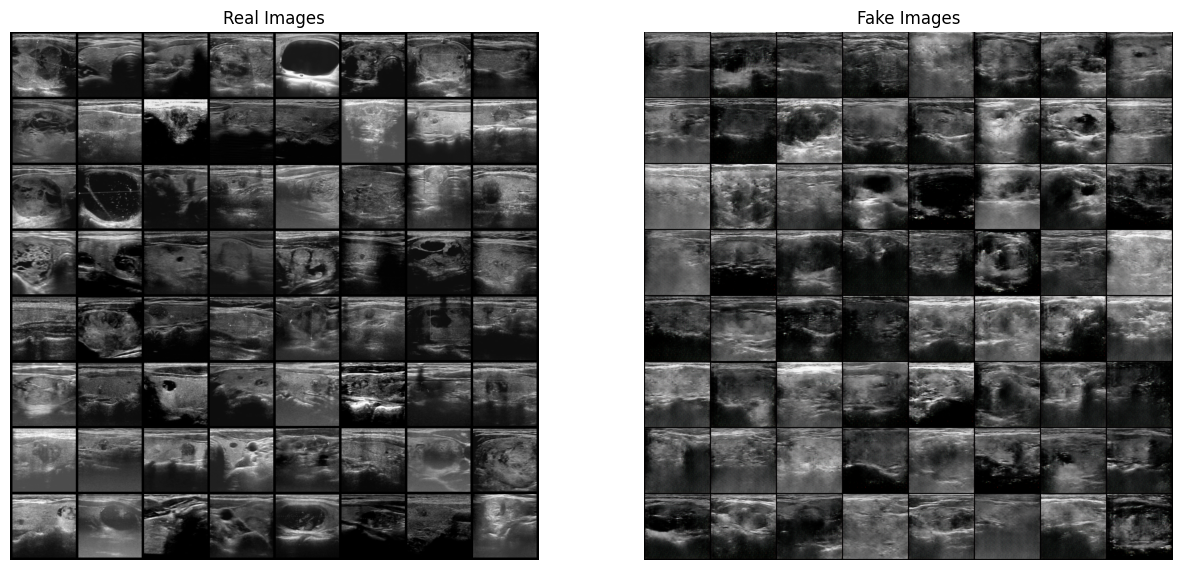
\includegraphics[width=0.85\textwidth]{4/figures/generated_real_1.png}
		\caption[Imágenes de ultrasonido de nódulos tiroideos generados y reales]{Imágenes de ultrasonido de nódulos tiroideos generados y reales. \\
		Fuente: Elaboración propia.}
		\label{4:fig115}
	\end{center}
\end{figure}

Según un rápido análisis visual, la imágenes generadas sí tienen un poco de similitud a las originales, y fácilmente, para alguien no experto, estos podrían pasar como imágenes reales.

Ya que el entrenamiento se realizó con todas las imágenes la data de entrenamiento, todas las imágenes generadas podrían pertenecer a cualquiera de las clases (benigno o maligno) y se es difícil sino imposible determinar a qué tipo pertenecen (benigno o maligno). Por este motivo, y viendo el potencial del DCGAN, se volvió a entrenar el modelo ahora solo con imágenes de la clase maligno (clase minoritaria) del conjunto de datos de entrenamiento para que la red solo pueda generar imágenes de ultrasonido de esta clase en específico.

En este caso se modificó el tamaño de vector latente a 300 y los features map base a 256 en la red generadora. Las demás configuraciones se mantuvieron, incluyendo aquellas de la red discriminadora.

Se usaron la misma función de pérdida y optimización con los mismos parámetros definidos anteriormente.

El tensor fijo de números aleatorio de distribución normal tuvo para este entrenamiento un tamaño de 300 (igual al tamaño del vector latente).

Para el DataLoader se mantuvo el mismo tamaño de redimensionamiento y lote.

Debido a una prueba rápida inicial con una menor cantidad de épocas, donde se obtuvieron pobres resultados, se decidió aumentar la cantidad de iteraciones totales estableciendo el número de épocas a 370.

La Figura \ref{4:fig116} muestra la parte final del entrenamiento.

\begin{figure}[H]
	\begin{center}
		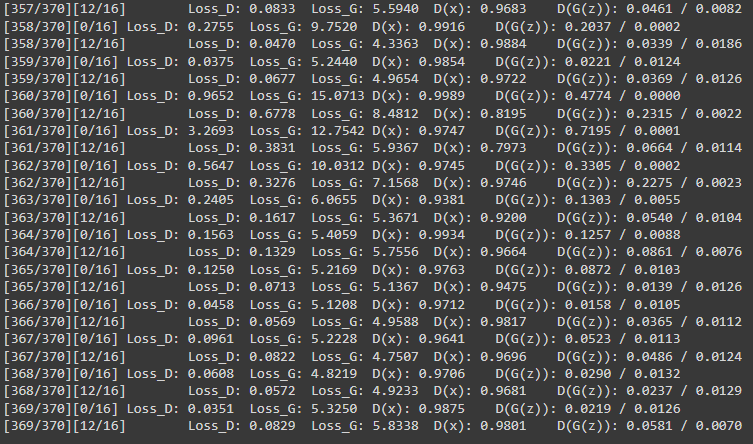
\includegraphics[width=0.75\textwidth]{4/figures/dcgan_2_train.PNG}
		\caption[Parte final del entrenamietno del DCGAN con imágenes de nódulos malignos]{Parte final del entrenamietno del DCGAN con imágenes de nódulos malignos. \\
		Fuente: Elaboración propia.}
		\label{4:fig116}
	\end{center}
\end{figure}

De igual manera al entrenamiento inicial, se realizó una gráfica donde se muestra el comportamiento de la pérdida en ambas redes. Esto se muestra en la Figura \ref{4:fig117}.

\begin{figure}[H]
	\begin{center}
		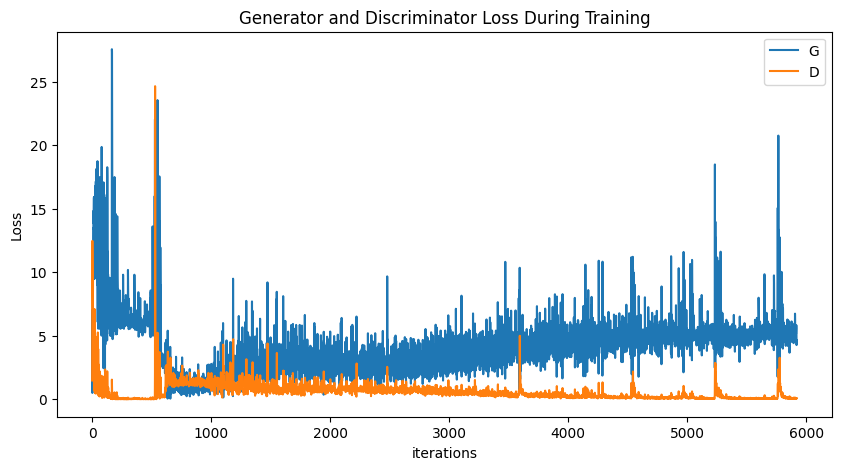
\includegraphics[width=0.85\textwidth]{4/figures/plot_loss_2.png}
		\caption[Plot de pérdidas de las red Generadora y Discriminadora de imágenes de nódulos malignos]{Plot de pérdidas de las red Generadora y Discriminadora de imágenes de nódulos malignos. \\
		Fuente: Elaboración propia.}
		\label{4:fig117}
	\end{center}
\end{figure}

Esta gráfica muestra el mismo comportamiento que a más iteraciones, mayor divergencia entre las pérdidas.

En la Figura \ref{4:fig118} se presentan las imágenes generadas junto a las originales.

\begin{figure}[H]
	\begin{center}
		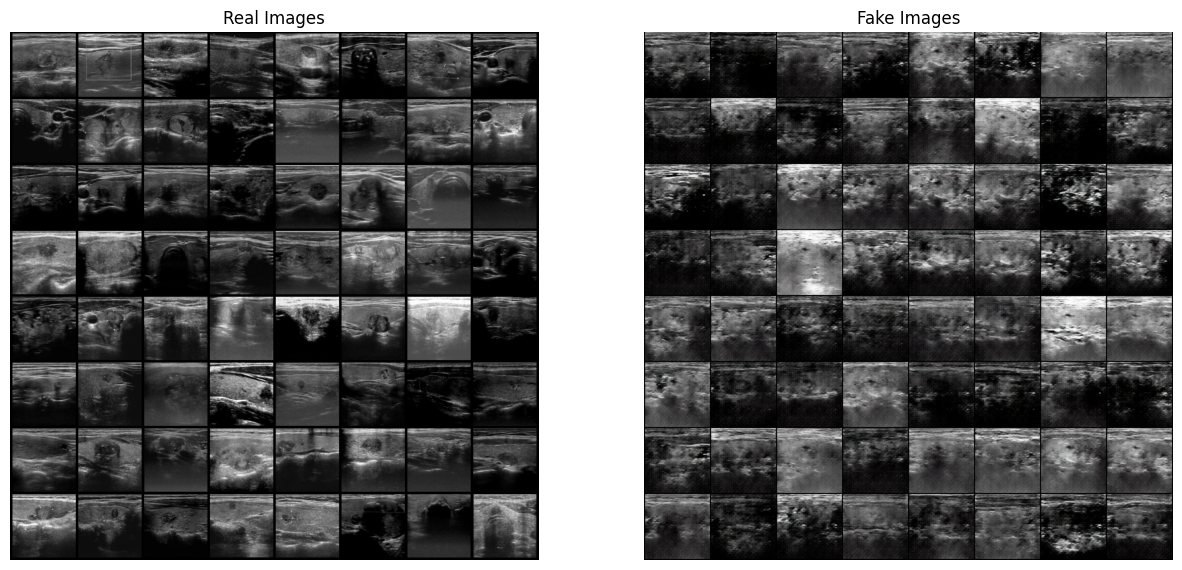
\includegraphics[width=0.85\textwidth]{4/figures/generated_real_2.png}
		\caption[Imágenes de ultrasonido de nódulos tiroideos generados y reales (DCGAN de imágenes de nódulos malignos)]{Imágenes de ultrasonido de nódulos tiroideos generados y reales (DCGAN de imágenes de nódulos malignos). \\
		Fuente: Elaboración propia.}
		\label{4:fig118}
	\end{center}
\end{figure}

Los resultados de las imágenes generadas en este modelo muestran mayor ruido comparado las generadas con el entrenamiento inicial, esto se debe principalmente a la menor cantidad de datos usada para el entrenamiento de este nuevo DCGAN. Sin embargo, luego de un rápido análisis visual, se puede observar un comportamiento similar entre todas estas imágenes nuevas, y es que en la mayoría de estas hay lo que parece ser la presencia de un nódulo, aunque difuminado con mucho ruido aleatorio, esto podría indicar un aprendizaje cercano a la distribución de las imágenes de nódulos malignos.

Intentando utilizar el potencial que ofrece el DCGAN, se realizó posteriormente dos tipos de entrenamiento a los modelos de Deep Learning: el primero sin el Aumento de Datos a través de DCGAN, mientras que el segundo combinará los datos generados con la data original de entrenamiento para realizar dicho proceso. Esto permitirá determinar si las imágenes generadas por el DCGAN, aunque con ruido, son capaces de aumentar la capacidad de predicción de los modelos.

La gráfica circula presenta en la Figura \ref{4:fig119} muestra el nuevo balance entre ambas clases en la nueva data de entrenamiento.

\begin{figure}[H]
	\begin{center}
		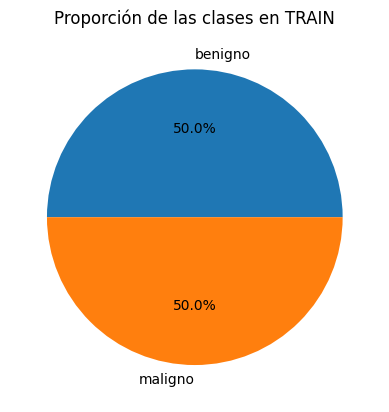
\includegraphics[width=0.51\textwidth]{4/figures/balanced_circular.png}
		\caption[Gráfica circula de data de entrenamiento balanceada]{Gráfica circula de data de entrenamiento balanceada. \\
		Fuente: Elaboración propia.}
		\label{4:fig119}
	\end{center}
\end{figure}

Ya con la data preprocesada, se inició con la etapa de Aplicación de Deep Learning donde se entrenó, validó y puso a prueba los diversos modelos CNN y ViT. Esta etapa inicia con la siguiente actividad.

\textbf{Actividad 1: Seleccionar algoritmos a entrenar según usos y resultados de las investigaciones presentadas en los antecedentes}
\\
Según los datos analizados en las investigaciones presentadas en el Capítulo 2, el modelo con mayor presencia de los CNN es el ResNet50, mientras que por el lado de los modelos ViT, los más usados son los ViT-Base con tamaño de patch de 16 x 16.

Además, debido al tipo de problema de clasificación presente en esta investigación, y la similitud con el trabajo de \cite{pr_JERBI2023autoclassViTGAN}, se decidió por probar con las redes VGG16, ya que ha demostrado ser capaz de obtener un alto desempeño.

En resumen, se ha optado por utilizar las arquitecturas CNN de ResNet50 y VGG16. Además, como parte de las arquitecturas ViT, se optó por el uso de ViT-Base (16).

\textbf{Actividad 2: Entrenar y probar los modelos de Deep Learning previamente definidos}
\\
Para todas las arquitecturas de Deep Learning en esta investigación, se definió como función de activación el sigmoide. De igual manera, para el entrenamiento se usó la capacidad de la GPU NVIDIA A100-SXM4-40GB obtenido a través de Google Colab para lograr un rápido y eficiente entrenamiento. Además, se determinó una semilla de 2024 para permitir la reproducibilidad de los resultados. 

En este primer grupo, no se utilizará el conjunto de datos con imágenes generadas.

Se empezó con los modelos ViT-Base (16).

Para este proceso se crearon los DataLoader correspondientes con las características requeridas por estos modelos ViT: se redimensionaron las imágenes a 224 x 224 y se definió un tamaño de lote de 64 (este último tamaño será constante para todos los modelos mostrados en esta actividad).

En este primer modelo, se usó la técnica de entrenamiento de Fine Tuning junto con el modelo ViT-Base (16) con pesos de IMAGENET1KV1.

La función de pérdida aplicada fue el BCEWithLogitsLoss que evita el uso manual de la sigmoide y lo aplica directamente con la entropía cruzada. Nuevamente, esta función será utilizada en cada uno de los modelos en esta actividad.

Para lograr una clasificación binaria, las últimas capas de estas arquitecturas debió ser reemplazada por un MLP simple que recibe todos los features del modelo y produce una única salida. La configuración del MLP se definió de la forma (256, 1), donde el primer valor es el número de neuronas en la capas oculta que tuvo la función de activación ReLU, y el segundo valor es el número de neuronas en la capa de salida. Esta configuración de MLP se aplicó a todos los modelos ViT y CNN, a excepción de VGG16, donde se usó una configuración por defecto, únicamente modificando a 1 el número de neuronas en la capa de salida. En el caso de los modelos híbridos, solamente se etableció el bloque clasificador a una capa de salida con 1 neurona, debido a las limitaciones de disponibilidad de recursos computacionales.

Finalmente, la función de optimización utilizada fue Adam con una tasa de aprendizaje de 0.0001, y se definió para el entrenamiento 20 épocas. Las demás configuraciones se dejaron por defecto.

Estas configuraciones se aplicarán de igual manera a los demás modelos en esta actividad.

A continuación se presenta en la Figura \ref{4:fig120} el proceso de entrenamiento del modelo ViT-Base (16) con los pesos IMAGENET1KV1 y usando la técnica de Fine Tuning.

\begin{figure}[H]
	\begin{center}
		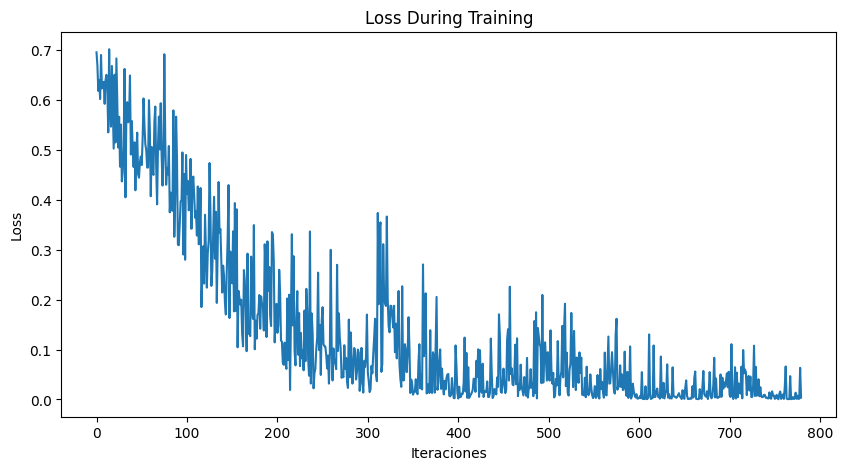
\includegraphics[width=0.85\textwidth]{4/figures/model1_train.PNG}
		\caption[Proceso de entrenamiento del modelo n°1]{Proceso de entrenamiento del modelo n°1. \\
		Fuente: Elaboración propia.}
		\label{4:fig120}
	\end{center}
\end{figure}

Finalmente, para este modelo también se calcularon su Accuracy, Recall y Precision. Estos son presentados en la Tabla \ref{4:table2}.

\begin{table}[H]
	\caption[Accuracy, Recall y Precision del modelo n°1]{Accuracy, Recall y Precision del modelo n°1.}
	\label{4:table2}
	\centering
	\small
	\begin{tabular}{c|ccc}
		\specialrule{.1em}{.05em}{.05em}
		{Métrica} & {Accuracy} & {Recall} & {Precision} \\
		\hline
		{Valor} & {69.54\%} & {47.03\%} & {64.16\%} \\
		\specialrule{.1em}{.05em}{.05em}
	\end{tabular}
	\begin{flushleft}	
		\small Fuente: Elaboración propia.
	\end{flushleft}
\end{table}

\begin{comment}
\begin{figure}[H]
	\begin{center}
		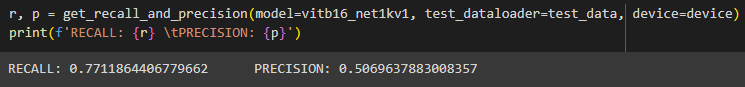
\includegraphics[width=0.83\textwidth]{4/figures/model1_rp.PNG}
		\caption[Accuracy, Recall y Precision del modelo n°1]{Recall y Precision del modelo n°1. \\
		Fuente: Elaboración propia.}
		\label{4:fig121}
	\end{center}
\end{figure}
\end{comment}

En el siguiente modelo, se usó la técnica de entrenamiento de Transfer Learning junto con el modelo ViT-Base (16) con pesos de IMAGENET1KV1.

El DataLoader constaba de las imágenes redimensionadas nuevamente a 224 x 224, y se aplicó la función de pérdida BCEWithLogitsLoss junto con la función de optimización Adam.

A continuación se presenta en la Figura \ref{4:fig122} el proceso de entrenamiento del modelo ViT-Base (16) con los pesos IMAGENET1KV1 y usando la técnica de Transfer Learning.

\begin{figure}[H]
	\begin{center}
		\includegraphics[width=0.85\textwidth]{4/figures/model2_train.PNG}
		\caption[Proceso de entrenamiento del modelo n°2]{Proceso de entrenamiento del modelo n°2. \\
		Fuente: Elaboración propia.}
		\label{4:fig122}
	\end{center}
\end{figure}

También se calcularon su Accuracy, Recall y Precision. Estos son presentados en la Tabla \ref{4:table3}.

\begin{table}[H]
	\caption[Accuracy, Recall y Precision del modelo n°2]{Accuracy, Recall y Precision del modelo n°2.}
	\label{4:table3}
	\centering
	\small
	\begin{tabular}{c|ccc}
		\specialrule{.1em}{.05em}{.05em}
		{Métrica} & {Accuracy} & {Recall} & {Precision} \\
		\hline
		{Valor} & {68.08\%} & {53.39\%} & {59.43\%} \\
		\specialrule{.1em}{.05em}{.05em}
	\end{tabular}
	\begin{flushleft}	
		\small Fuente: Elaboración propia.
	\end{flushleft}
\end{table}

\begin{comment}
\begin{figure}[H]
	\begin{center}
		\includegraphics[width=0.83\textwidth]{4/figures/model2_rp.PNG}
		\caption[Recall y Precision del modelo n°2]{Recall y Precision del modelo n°2. \\
		Fuente: Elaboración propia.}
		\label{4:fig123}
	\end{center}
\end{figure}
\end{comment}

Este modelo usó la técnica de entrenamiento de Fine Tuning junto con el modelo ViT-Base (16) con pesos de IMAGENET1KSWAGE2EV1.

En este caso, el DataLoader constaba de las imágenes redimensionadas a 384 x 384.

Se presenta en la Figura \ref{4:fig124} el proceso de entrenamiento del modelo ViT-Base (16) con los pesos  IMAGENET1KSWAGE2EV1 y usando la técnica de Fine Tuning.

\begin{figure}[H]
	\begin{center}
		\includegraphics[width=0.85\textwidth]{4/figures/model3_train.PNG}
		\caption[Proceso de entrenamiento del modelo n°3]{Proceso de entrenamiento del modelo n°3. \\
		Fuente: Elaboración propia.}
		\label{4:fig124}
	\end{center}
\end{figure}

También se calcularon su Accuracy, Recall y Precision. Estos son presentados en la Tabla \ref{4:table4}.

\begin{table}[H]
	\caption[Accuracy, Recall y Precision del modelo n°3]{Accuracy, Recall y Precision del modelo n°3.}
	\label{4:table4}
	\centering
	\small
	\begin{tabular}{c|ccc}
		\specialrule{.1em}{.05em}{.05em}
		{Métrica} & {Accuracy} & {Recall} & {Precision} \\
		\hline
		{Valor} & {56.84\%} & {53.81\%} & {44.88\%} \\
		\specialrule{.1em}{.05em}{.05em}
	\end{tabular}
	\begin{flushleft}	
		\small Fuente: Elaboración propia.
	\end{flushleft}
\end{table}

\begin{comment}
\begin{figure}[H]
	\begin{center}
		\includegraphics[width=0.83\textwidth]{4/figures/model3_rp.PNG}
		\caption[Recall y Precision del modelo n°3]{Recall y Precision del modelo n°3. \\
		Fuente: Elaboración propia.}
		\label{4:fig125}
	\end{center}
\end{figure}
\end{comment}

El modelo n°4 empleó la técnica de entrenamiento de Transfer Learning junto con el modelo ViT-Base (16) con pesos de IMAGENET1KSWAGE2EV1.

En este caso, nuevamente el DataLoader constaba de las imágenes redimensionadas a 384 x 384.

Se presenta en la Figura \ref{4:fig126} el proceso de entrenamiento del modelo ViT-Base (16) con los pesos IMAGENET1KSWAGE2EV1 y usando la técnica de Transfer Learning.

\begin{figure}[H]
	\begin{center}
		\includegraphics[width=0.85\textwidth]{4/figures/model4_train.PNG}
		\caption[Proceso de entrenamiento del modelo n°4]{Proceso de entrenamiento del modelo n°4. \\
		Fuente: Elaboración propia.}
		\label{4:fig126}
	\end{center}
\end{figure}

También se calcularon su Accuracy, Recall y Precision. Estos son presentados en la Tabla \ref{4:table5}.

\begin{table}[H]
	\caption[Accuracy, Recall y Precision del modelo n°4]{Accuracy, Recall y Precision del modelo n°4.}
	\label{4:table5}
	\centering
	\small
	\begin{tabular}{c|ccc}
		\specialrule{.1em}{.05em}{.05em}
		{Métrica} & {Accuracy} & {Recall} & {Precision} \\
		\hline
		{Valor} & {69.22\%} & {55.51\%} & {60.93\%} \\
		\specialrule{.1em}{.05em}{.05em}
	\end{tabular}
	\begin{flushleft}	
		\small Fuente: Elaboración propia.
	\end{flushleft}
\end{table}

\begin{comment}
\begin{figure}[H]
	\begin{center}
		\includegraphics[width=0.83\textwidth]{4/figures/model4_rp.PNG}
		\caption[Recall y Precision del modelo n°4]{Recall y Precision del modelo n°4. \\
		Fuente: Elaboración propia.}
		\label{4:fig127}
	\end{center}
\end{figure}
\end{comment}

El modelo n°5 empleó la técnica de entrenamiento de Fine Tuning junto con el modelo ViT-Base (16) con pesos de IMAGENET1KSWAGLINEARV1.

En este caso, el DataLoader constaba de las imágenes redimensionadas a 224 x 224.

Se presenta en la Figura \ref{4:fig128} el proceso de entrenamiento del modelo ViT-Base (16) con los pesos IMAGENET1KSWAGLINEARV1 y usando la técnica de Fine Tuning.

\begin{figure}[H]
	\begin{center}
		\includegraphics[width=0.85\textwidth]{4/figures/model5_train.PNG}
		\caption[Proceso de entrenamiento del modelo n°5]{Proceso de entrenamiento del modelo n°5. \\
		Fuente: Elaboración propia.}
		\label{4:fig128}
	\end{center}
\end{figure}

También se calcularon su Recall y Precision. Estos son presentados en la Tabla \ref{4:table6}.

\begin{table}[H]
	\caption[Accuracy, Recall y Precision del modelo n°5]{Accuracy, Recall y Precision del modelo n°5.}
	\label{4:table6}
	\centering
	\small
	\begin{tabular}{c|ccc}
		\specialrule{.1em}{.05em}{.05em}
		{Métrica} & {Accuracy} & {Recall} & {Precision} \\
		\hline
		{Valor} & {58.47\%} & {34.75\%} & {44.81\%} \\
		\specialrule{.1em}{.05em}{.05em}
	\end{tabular}
	\begin{flushleft}	
		\small Fuente: Elaboración propia.
	\end{flushleft}
\end{table}

\begin{comment}
\begin{figure}[H]
	\begin{center}
		\includegraphics[width=0.83\textwidth]{4/figures/model5_rp.PNG}
		\caption[Recall y Precision del modelo n°5]{Recall y Precision del modelo n°5. \\
		Fuente: Elaboración propia.}
		\label{4:fig129}
	\end{center}
\end{figure}
\end{comment}

El modelo n°6 empleó la técnica de entrenamiento de Transfer Learning junto con el modelo ViT-Base (16) con pesos de IMAGENET1KSWAGLINEARV1.

En este caso, el DataLoader constaba nuevamente de las imágenes redimensionadas a 224 x 224.

Se presenta en la Figura \ref{4:fig130} el proceso de entrenamiento del modelo ViT-Base (16) con los pesos IMAGENET1KSWAGLINEARV1 y usando la técnica de Transfer Learning.

\begin{figure}[H]
	\begin{center}
		\includegraphics[width=0.85\textwidth]{4/figures/model6_train.PNG}
		\caption[Proceso de entrenamiento del modelo n°6]{Proceso de entrenamiento del modelo n°6. \\
		Fuente: Elaboración propia.}
		\label{4:fig130}
	\end{center}
\end{figure}

También se calcularon su Accuracy, Recall y Precision. Estos son presentados en la Tabla \ref{4:table7}.

\begin{table}[H]
	\caption[Accuracy, Recall y Precision del modelo n°6]{Accuracy, Recall y Precision del modelo n°6.}
	\label{4:table7}
	\centering
	\small
	\begin{tabular}{c|ccc}
		\specialrule{.1em}{.05em}{.05em}
		{Métrica} & {Accuracy} & {Recall} & {Precision} \\
		\hline
		{Valor} & {65.31\%} & {41.95\%} & {56.57\%} \\
		\specialrule{.1em}{.05em}{.05em}
	\end{tabular}
	\begin{flushleft}	
		\small Fuente: Elaboración propia.
	\end{flushleft}
\end{table}

\begin{comment}
\begin{figure}[H]
	\begin{center}
		\includegraphics[width=0.83\textwidth]{4/figures/model6_rp.PNG}
		\caption[Recall y Precision del modelo n°6]{Recall y Precision del modelo n°6. \\
		Fuente: Elaboración propia.}
		\label{4:fig131}
	\end{center}
\end{figure}
\end{comment}

El modelo n°7 empleó la técnica de entrenamiento de Fine Tuning junto con el modelo VGG16 con pesos de IMAGENET1KV1.

En este caso, el DataLoader fue cargado con imágenes redimensionadas a 128 x 128. Este tamaño será constante para los demás modelos CNN.

Se presenta en la Figura \ref{4:fig132} el proceso de entrenamiento del modelo VGG16 con los pesos IMAGENET1KV1 y usando la técnica de Fine Tuning.

\begin{figure}[H]
	\begin{center}
		\includegraphics[width=0.85\textwidth]{4/figures/model7_train.PNG}
		\caption[Proceso de entrenamiento del modelo n°7]{Proceso de entrenamiento del modelo n°7. \\
		Fuente: Elaboración propia.}
		\label{4:fig132}
	\end{center}
\end{figure}

También se calcularon su Accuracy, Recall y Precision. Estos son presentados en la Tabla \ref{4:table8}.

\begin{table}[H]
	\caption[Accuracy, Recall y Precision del modelo n°7]{Accuracy, Recall y Precision del modelo n°7.}
	\label{4:table8}
	\centering
	\small
	\begin{tabular}{c|ccc}
		\specialrule{.1em}{.05em}{.05em}
		{Métrica} & {Accuracy} & {Recall} & {Precision} \\
		\hline
		{Valor} & {71.99\%} & {58.90\%} & {64.95\%} \\
		\specialrule{.1em}{.05em}{.05em}
	\end{tabular}
	\begin{flushleft}	
		\small Fuente: Elaboración propia.
	\end{flushleft}
\end{table}

\begin{comment}
\begin{figure}[H]
	\begin{center}
		\includegraphics[width=0.83\textwidth]{4/figures/model7_rp.PNG}
		\caption[Recall y Precision del modelo n°7]{Recall y Precision del modelo n°7. \\
		Fuente: Elaboración propia.}
		\label{4:fig133}
	\end{center}
\end{figure}
\end{comment}

El modelo n°8 empleó la técnica de entrenamiento de Transfer Learning junto con el modelo VGG16 con pesos de IMAGENET1KV1.

Se presenta en la Figura \ref{4:fig134} el proceso del entrenamiento del modelo VGG16 con los pesos IMAGENET1KV1 y usando la técnica de Transfer Learning.

\begin{figure}[H]
	\begin{center}
		\includegraphics[width=0.85\textwidth]{4/figures/model8_train.PNG}
		\caption[Proceso de entrenamiento del modelo n°8]{Proceso de entrenamiento del modelo n°8. \\
		Fuente: Elaboración propia.}
		\label{4:fig134}
	\end{center}
\end{figure}

También se calcularon su Accuracy, Recall y Precision. Estos son presentados en la Tabla \ref{4:table9}.

\begin{table}[H]
	\caption[Accuracy, Recall y Precision del modelo n°8]{Accuracy, Recall y Precision del modelo n°8.}
	\label{4:table9}
	\centering
	\small
	\begin{tabular}{c|ccc}
		\specialrule{.1em}{.05em}{.05em}
		{Métrica} & {Accuracy} & {Recall} & {Precision} \\
		\hline
		{Valor} & {65.80\%} & {67.37\%} & {54.45\%} \\
		\specialrule{.1em}{.05em}{.05em}
	\end{tabular}
	\begin{flushleft}	
		\small Fuente: Elaboración propia.
	\end{flushleft}
\end{table}

\begin{comment}
\begin{figure}[H]
	\begin{center}
		\includegraphics[width=0.83\textwidth]{4/figures/model8_rp.PNG}
		\caption[Recall y Precision del modelo n°8]{Recall y Precision del modelo n°8. \\
		Fuente: Elaboración propia.}
		\label{4:fig135}
	\end{center}
\end{figure}
\end{comment}

El modelo n°9 empleó la técnica de entrenamiento de Fine Tuning junto con el modelo RESNET50 con pesos de IMAGENET1KV1.

Se presenta en la Figura \ref{4:fig136} el proceso del entrenamiento del modelo RESNET50 con los pesos IMAGENET1KV1 y usando la técnica de Fine Tuning.

\begin{figure}[H]
	\begin{center}
		\includegraphics[width=0.85\textwidth]{4/figures/model9_train.PNG}
		\caption[Proceso de entrenamiento del modelo n°9]{Proceso de entrenamiento del modelo n°9. \\
		Fuente: Elaboración propia.}
		\label{4:fig136}
	\end{center}
\end{figure}

También se calcularon su Accuracy, Recall y Precision. Estos son presentados en la Tabla \ref{4:table10}.

\begin{table}[H]
	\caption[Accuracy, Recall y Precision del modelo n°9]{Accuracy, Recall y Precision del modelo n°9.}
	\label{4:table10}
	\centering
	\small
	\begin{tabular}{c|ccc}
		\specialrule{.1em}{.05em}{.05em}
		{Métrica} & {Accuracy} & {Recall} & {Precision} \\
		\hline
		{Valor} & {72.48\%} & {58.90\%} & {65.88\%} \\
		\specialrule{.1em}{.05em}{.05em}
	\end{tabular}
	\begin{flushleft}	
		\small Fuente: Elaboración propia.
	\end{flushleft}
\end{table}

\begin{comment}
\begin{figure}[H]
	\begin{center}
		\includegraphics[width=0.83\textwidth]{4/figures/model9_rp.PNG}
		\caption[Recall y Precision del modelo n°9]{Recall y Precision del modelo n°9. \\
		Fuente: Elaboración propia.}
		\label{4:fig137}
	\end{center}
\end{figure}
\end{comment}

El modelo n°10 empleó la técnica de entrenamiento de Transfer Learning  junto con el modelo RESNET50 con pesos de IMAGENET1KV1.

Se presenta en la Figura \ref{4:fig138} el proceso del entrenamiento del modelo RESNET50 con los pesos IMAGENET1KV1 y usando la técnica de Transfer Learning.

\begin{figure}[H]
	\begin{center}
		\includegraphics[width=0.85\textwidth]{4/figures/model10_train.PNG}
		\caption[Proceso de entrenamiento del modelo n°10]{Proceso de entrenamiento del modelo n°10. \\
		Fuente: Elaboración propia.}
		\label{4:fig138}
	\end{center}
\end{figure}

También se calcularon su Accuracy, Recall y Precision. Estos son presentados en la Tabla \ref{4:table11}.

\begin{table}[H]
	\caption[Accuracy, Recall y Precision del modelo n°10]{Accuracy, Recall y Precision del modelo n°10.}
	\label{4:table11}
	\centering
	\small
	\begin{tabular}{c|ccc}
		\specialrule{.1em}{.05em}{.05em}
		{Métrica} & {Accuracy} & {Recall} & {Precision} \\
		\hline
		{Valor} & {62.38\%} & {37.71\%} & {51.45\%} \\
		\specialrule{.1em}{.05em}{.05em}
	\end{tabular}
	\begin{flushleft}	
		\small Fuente: Elaboración propia.
	\end{flushleft}
\end{table}

\begin{comment}
\begin{figure}[H]
	\begin{center}
		\includegraphics[width=0.83\textwidth]{4/figures/model10_rp.PNG}
		\caption[Recall y Precision del modelo n°10]{Recall y Precision del modelo n°10. \\
		Fuente: Elaboración propia.}
		\label{4:fig139}
	\end{center}
\end{figure}
\end{comment}

El modelo n°11 empleó la técnica de entrenamiento de Fine Tuning junto con el modelo RESNET50 con pesos de IMAGENET1KV2.

Se presenta en la Figura \ref{4:fig140} el proceso del entrenamiento del modelo RESNET50 con los pesos IMAGENET1KV2 y usando la técnica de Fine Tuning.

\begin{figure}[H]
	\begin{center}
		\includegraphics[width=0.85\textwidth]{4/figures/model11_train.PNG}
		\caption[Proceso de entrenamiento del modelo n°11]{Proceso de entrenamiento del modelo n°11. \\
		Fuente: Elaboración propia.}
		\label{4:fig140}
	\end{center}
\end{figure}

También se calcularon su Accuracy, Recall y Precision. Estos son presentados en la Tabla \ref{4:table12}.

\begin{table}[H]
	\caption[Accuracy, Recall y Precision del modelo n°11]{Accuracy, Recall y Precision del modelo n°11.}
	\label{4:table12}
	\centering
	\small
	\begin{tabular}{c|ccc}
		\specialrule{.1em}{.05em}{.05em}
		{Métrica} & {Accuracy} & {Recall} & {Precision} \\
		\hline
		{Valor} & {67.59\%} & {51.27\%} & {59.02\%} \\
		\specialrule{.1em}{.05em}{.05em}
	\end{tabular}
	\begin{flushleft}	
		\small Fuente: Elaboración propia.
	\end{flushleft}
\end{table}

\begin{comment}
\begin{figure}[H]
	\begin{center}
		\includegraphics[width=0.83\textwidth]{4/figures/model11_rp.PNG}
		\caption[Recall y Precision del modelo n°11]{Recall y Precision del modelo n°11. \\
		Fuente: Elaboración propia.}
		\label{4:fig141}
	\end{center}
\end{figure}
\end{comment}

El modelo n°12 empleó la técnica de entrenamiento de Transfer Learning junto con el modelo RESNET50 con pesos de IMAGENET1KV2.

Se presenta en la Figura \ref{4:fig142} el proceso del entrenamiento del modelo RESNET50 con los pesos IMAGENET1KV2 y usando la técnica de Transfer Learning.

\begin{figure}[H]
	\begin{center}
		\includegraphics[width=0.85\textwidth]{4/figures/model12_train.PNG}
		\caption[Proceso de entrenamiento del modelo n°12]{Proceso de entrenamiento del modelo n°12. \\
		Fuente: Elaboración propia.}
		\label{4:fig142}
	\end{center}
\end{figure}

También se calcularon su Accuracy, Recall y Precision. Estos son presentados en la Tabla \ref{4:table13}.

\begin{table}[H]
	\caption[Accuracy, Recall y Precision del modelo n°12]{Accuracy, Recall y Precision del modelo n°12.}
	\label{4:table13}
	\centering
	\small
	\begin{tabular}{c|ccc}
		\specialrule{.1em}{.05em}{.05em}
		{Métrica} & {Accuracy} & {Recall} & {Precision} \\
		\hline
		{Valor} & {62.05\%} & {49.15\%} & {50.66\%} \\
		\specialrule{.1em}{.05em}{.05em}
	\end{tabular}
	\begin{flushleft}	
		\small Fuente: Elaboración propia.
	\end{flushleft}
\end{table}

\begin{comment}
\begin{figure}[H]
	\begin{center}
		\includegraphics[width=0.83\textwidth]{4/figures/model12_rp.PNG}
		\caption[Recall y Precision del modelo n°12]{Recall y Precision del modelo n°12. \\
		Fuente: Elaboración propia.}
		\label{4:fig143}
	\end{center}
\end{figure}
\end{comment}

Una vez culminado el entrenamiento de los modelos con el conjunto de datos sin imágenes generadas, se inició un nuevo proceso de entrenamiento, esta vez con el conjunto de datos aumentado. 

Todos los modelos, tanto ViT como CNN, poseen las mismas configuraciones definidas antes, así que no hay necesidad de especificarlo nuevamente.

A continuación se presentan las siguientes Figuras y Tablas donde se muestran todos los resultados de los modelos de manera similar a como se presentó anteriormente.

\begin{figure}[H]
	\begin{center}
		\includegraphics[width=0.85\textwidth]{4/figures/model13_train.PNG}
		\caption[Proceso de entrenamiento del modelo n°13]{Proceso de entrenamiento del modelo n°13. \\
		Fuente: Elaboración propia.}
		\label{4:fig144}
	\end{center}
\end{figure}

\begin{table}[H]
	\caption[Accuracy, Recall y Precision del modelo n°13]{Accuracy, Recall y Precision del modelo n°13.}
	\label{4:table14}
	\centering
	\small
	\begin{tabular}{c|ccc}
		\specialrule{.1em}{.05em}{.05em}
		{Métrica} & {Accuracy} & {Recall} & {Precision} \\
		\hline
		{Valor} & {70.36\%} & {61.44\%} & {61.44\%} \\
		\specialrule{.1em}{.05em}{.05em}
	\end{tabular}
	\begin{flushleft}	
		\small Fuente: Elaboración propia.
	\end{flushleft}
\end{table}

\begin{comment}
\begin{figure}[H]
	\begin{center}
		\includegraphics[width=0.83\textwidth]{4/figures/model13_rp.PNG}
		\caption[Recall y Precision del modelo n°13]{Recall y Precision del modelo n°13. \\
		Fuente: Elaboración propia.}
		\label{4:fig145}
	\end{center}
\end{figure}
\end{comment}

\begin{figure}[H]
	\begin{center}
		\includegraphics[width=0.85\textwidth]{4/figures/model14_train.PNG}
		\caption[Proceso de entrenamiento del modelo n°14]{Proceso de entrenamiento del modelo n°14. \\
		Fuente: Elaboración propia.}
		\label{4:fig146}
	\end{center}
\end{figure}

\begin{table}[H]
	\caption[Accuracy, Recall y Precision del modelo n°14]{Accuracy, Recall y Precision del modelo n°14.}
	\label{4:table15}
	\centering
	\small
	\begin{tabular}{c|ccc}
		\specialrule{.1em}{.05em}{.05em}
		{Métrica} & {Accuracy} & {Recall} & {Precision} \\
		\hline
		{Valor} & {69.06\%} & {50.00\%} & {62.11\%} \\
		\specialrule{.1em}{.05em}{.05em}
	\end{tabular}
	\begin{flushleft}	
		\small Fuente: Elaboración propia.
	\end{flushleft}
\end{table}

\begin{comment}
\begin{figure}[H]
	\begin{center}
		\includegraphics[width=0.83\textwidth]{4/figures/model14_rp.PNG}
		\caption[Recall y Precision del modelo n°14]{Recall y Precision del modelo n°14. \\
		Fuente: Elaboración propia.}
		\label{4:fig147}
	\end{center}
\end{figure}
\end{comment}

\begin{figure}[H]
	\begin{center}
		\includegraphics[width=0.85\textwidth]{4/figures/model15_train.PNG}
		\caption[Proceso de entrenamiento del modelo n°15]{Proceso de entrenamiento del modelo n°15. \\
		Fuente: Elaboración propia.}
		\label{4:fig148}
	\end{center}
\end{figure}

\begin{table}[H]
	\caption[Accuracy, Recall y Precision del modelo n°15]{Accuracy, Recall y Precision del modelo n°15.}
	\label{4:table16}
	\centering
	\small
	\begin{tabular}{c|ccc}
		\specialrule{.1em}{.05em}{.05em}
		{Métrica} & {Accuracy} & {Recall} & {Precision} \\
		\hline
		{Valor} & {67.43\%} & {41.10\%} & {61.39\%} \\
		\specialrule{.1em}{.05em}{.05em}
	\end{tabular}
	\begin{flushleft}	
		\small Fuente: Elaboración propia.
	\end{flushleft}
\end{table}

\begin{comment}
\begin{figure}[H]
	\begin{center}
		\includegraphics[width=0.83\textwidth]{4/figures/model15_rp.PNG}
		\caption[Recall y Precision del modelo n°15]{Recall y Precision del modelo n°15. \\
		Fuente: Elaboración propia.}
		\label{4:fig149}
	\end{center}
\end{figure}
\end{comment}

\begin{figure}[H]
	\begin{center}
		\includegraphics[width=0.85\textwidth]{4/figures/model16_train.PNG}
		\caption[Proceso de entrenamiento del modelo n°16]{Proceso de entrenamiento del modelo n°16. \\
		Fuente: Elaboración propia.}
		\label{4:fig150}
	\end{center}
\end{figure}

\begin{table}[H]
	\caption[Accuracy, Recall y Precision del modelo n°16]{Accuracy, Recall y Precision del modelo n°16.}
	\label{4:table17}
	\centering
	\small
	\begin{tabular}{c|ccc}
		\specialrule{.1em}{.05em}{.05em}
		{Métrica} & {Accuracy} & {Recall} & {Precision} \\
		\hline
		{Valor} & {69.71\%} & {64.83\%} & {59.77\%} \\
		\specialrule{.1em}{.05em}{.05em}
	\end{tabular}
	\begin{flushleft}	
		\small Fuente: Elaboración propia.
	\end{flushleft}
\end{table}

\begin{comment}
\begin{figure}[H]
	\begin{center}
		\includegraphics[width=0.83\textwidth]{4/figures/model16_rp.PNG}
		\caption[Recall y Precision del modelo n°16]{Recall y Precision del modelo n°16. \\
		Fuente: Elaboración propia.}
		\label{4:fig151}
	\end{center}
\end{figure}
\end{comment}

\begin{figure}[H]
	\begin{center}
		\includegraphics[width=0.85\textwidth]{4/figures/model17_train.PNG}
		\caption[Proceso de entrenamiento del modelo n°17]{Proceso de entrenamiento del modelo n°17. \\
		Fuente: Elaboración propia.}
		\label{4:fig152}
	\end{center}
\end{figure}

\begin{table}[H]
	\caption[Accuracy, Recall y Precision del modelo n°17]{Accuracy, Recall y Precision del modelo n°17.}
	\label{4:table18}
	\centering
	\small
	\begin{tabular}{c|ccc}
		\specialrule{.1em}{.05em}{.05em}
		{Métrica} & {Accuracy} & {Recall} & {Precision} \\
		\hline
		{Valor} & {57.65\%} & {41.95\%} & {44.59\%} \\
		\specialrule{.1em}{.05em}{.05em}
	\end{tabular}
	\begin{flushleft}	
		\small Fuente: Elaboración propia.
	\end{flushleft}
\end{table}

\begin{comment}
\begin{figure}[H]
	\begin{center}
		\includegraphics[width=0.83\textwidth]{4/figures/model17_rp.PNG}
		\caption[Recall y Precision del modelo n°17]{Recall y Precision del modelo n°17. \\
		Fuente: Elaboración propia.}
		\label{4:fig153}
	\end{center}
\end{figure}
\end{comment}

\begin{figure}[H]
	\begin{center}
		\includegraphics[width=0.85\textwidth]{4/figures/model18_train.PNG}
		\caption[Proceso de entrenamiento del modelo n°18]{Proceso de entrenamiento del modelo n°18. \\
		Fuente: Elaboración propia.}
		\label{4:fig154}
	\end{center}
\end{figure}

\begin{table}[H]
	\caption[Accuracy, Recall y Precision del modelo n°18]{Accuracy, Recall y Precision del modelo n°18.}
	\label{4:table19}
	\centering
	\small
	\begin{tabular}{c|ccc}
		\specialrule{.1em}{.05em}{.05em}
		{Métrica} & {Accuracy} & {Recall} & {Precision} \\
		\hline
		{Valor} & {64.82\%} & {49.58\%} & {54.67\%} \\
		\specialrule{.1em}{.05em}{.05em}
	\end{tabular}
	\begin{flushleft}	
		\small Fuente: Elaboración propia.
	\end{flushleft}
\end{table}

\begin{comment}
\begin{figure}[H]
	\begin{center}
		\includegraphics[width=0.83\textwidth]{4/figures/model18_rp.PNG}
		\caption[Recall y Precision del modelo n°18]{Recall y Precision del modelo n°18. \\
		Fuente: Elaboración propia.}
		\label{4:fig155}
	\end{center}
\end{figure}
\end{comment}

\begin{figure}[H]
	\begin{center}
		\includegraphics[width=0.85\textwidth]{4/figures/model19_train.PNG}
		\caption[Proceso de entrenamiento del modelo n°19]{Proceso de entrenamiento del modelo n°19. \\
		Fuente: Elaboración propia.}
		\label{4:fig156}
	\end{center}
\end{figure}

\begin{table}[H]
	\caption[Accuracy, Recall y Precision del modelo n°19]{Accuracy, Recall y Precision del modelo n°19.}
	\label{4:table20}
	\centering
	\small
	\begin{tabular}{c|ccc}
		\specialrule{.1em}{.05em}{.05em}
		{Métrica} & {Accuracy} & {Recall} & {Precision} \\
		\hline
		{Valor} & {71.99\%} & {59.75\%} & {64.68\%} \\
		\specialrule{.1em}{.05em}{.05em}
	\end{tabular}
	\begin{flushleft}	
		\small Fuente: Elaboración propia.
	\end{flushleft}
\end{table}

\begin{comment}
\begin{figure}[H]
	\begin{center}
		\includegraphics[width=0.83\textwidth]{4/figures/model19_rp.PNG}
		\caption[Recall y Precision del modelo n°19]{Recall y Precision del modelo n°19. \\
		Fuente: Elaboración propia.}
		\label{4:fig157}
	\end{center}
\end{figure}
\end{comment}

\begin{figure}[H]
	\begin{center}
		\includegraphics[width=0.85\textwidth]{4/figures/model20_train.PNG}
		\caption[Proceso de entrenamiento del modelo n°20]{Proceso de entrenamiento del modelo n°20. \\
		Fuente: Elaboración propia.}
		\label{4:fig158}
	\end{center}
\end{figure}

\begin{table}[H]
	\caption[Accuracy, Recall y Precision del modelo n°20]{Accuracy, Recall y Precision del modelo n°20.}
	\label{4:table21}
	\centering
	\small
	\begin{tabular}{c|ccc}
		\specialrule{.1em}{.05em}{.05em}
		{Métrica} & {Accuracy} & {Recall} & {Precision} \\
		\hline
		{Valor} & {66.45\%} & {52.97\%} & {56.82\%} \\
		\specialrule{.1em}{.05em}{.05em}
	\end{tabular}
	\begin{flushleft}	
		\small Fuente: Elaboración propia.
	\end{flushleft}
\end{table}

\begin{comment}
\begin{figure}[H]
	\begin{center}
		\includegraphics[width=0.83\textwidth]{4/figures/model20_rp.PNG}
		\caption[Recall y Precision del modelo n°20]{Recall y Precision del modelo n°20. \\
		Fuente: Elaboración propia.}
		\label{4:fig159}
	\end{center}
\end{figure}
\end{comment}

\begin{figure}[H]
	\begin{center}
		\includegraphics[width=0.85\textwidth]{4/figures/model21_train.PNG}
		\caption[Proceso de entrenamiento del modelo n°21]{Proceso de entrenamiento del modelo n°21. \\
		Fuente: Elaboración propia.}
		\label{4:fig160}
	\end{center}
\end{figure}

\begin{table}[H]
	\caption[Accuracy, Recall y Precision del modelo n°21]{Accuracy, Recall y Precision del modelo n°21.}
	\label{4:table22}
	\centering
	\small
	\begin{tabular}{c|ccc}
		\specialrule{.1em}{.05em}{.05em}
		{Métrica} & {Accuracy} & {Recall} & {Precision} \\
		\hline
		{Valor} & {70.85\%} & {68.22\%} & {60.75\%} \\
		\specialrule{.1em}{.05em}{.05em}
	\end{tabular}
	\begin{flushleft}	
		\small Fuente: Elaboración propia.
	\end{flushleft}
\end{table}

\begin{comment}
\begin{figure}[H]
	\begin{center}
		\includegraphics[width=0.83\textwidth]{4/figures/model21_rp.PNG}
		\caption[Recall y Precision del modelo n°21]{Recall y Precision del modelo n°21. \\
		Fuente: Elaboración propia.}
		\label{4:fig161}
	\end{center}
\end{figure}
\end{comment}

\begin{figure}[H]
	\begin{center}
		\includegraphics[width=0.85\textwidth]{4/figures/model22_train.PNG}
		\caption[Proceso de entrenamiento del modelo n°22]{Proceso de entrenamiento del modelo n°22. \\
		Fuente: Elaboración propia.}
		\label{4:fig162}
	\end{center}
\end{figure}

\begin{table}[H]
	\caption[Accuracy, Recall y Precision del modelo n°22]{Accuracy, Recall y Precision del modelo n°22.}
	\label{4:table23}
	\centering
	\small
	\begin{tabular}{c|ccc}
		\specialrule{.1em}{.05em}{.05em}
		{Métrica} & {Accuracy} & {Recall} & {Precision} \\
		\hline
		{Valor} & {64.17\%} & {33.90\%} & {55.56\%} \\
		\specialrule{.1em}{.05em}{.05em}
	\end{tabular}
	\begin{flushleft}	
		\small Fuente: Elaboración propia.
	\end{flushleft}
\end{table}

\begin{comment}
\begin{figure}[H]
	\begin{center}
		\includegraphics[width=0.83\textwidth]{4/figures/model22_rp.PNG}
		\caption[Recall y Precision del modelo n°22]{Recall y Precision del modelo n°22. \\
		Fuente: Elaboración propia.}
		\label{4:fig163}
	\end{center}
\end{figure}
\end{comment}

\begin{figure}[H]
	\begin{center}
		\includegraphics[width=0.85\textwidth]{4/figures/model23_train.PNG}
		\caption[Proceso de entrenamiento del modelo n°23]{Proceso de entrenamiento del modelo n°23. \\
		Fuente: Elaboración propia.}
		\label{4:fig164}
	\end{center}
\end{figure}

\begin{table}[H]
	\caption[Accuracy, Recall y Precision del modelo n°23]{Accuracy, Recall y Precision del modelo n°23.}
	\label{4:table24}
	\centering
	\small
	\begin{tabular}{c|ccc}
		\specialrule{.1em}{.05em}{.05em}
		{Métrica} & {Accuracy} & {Recall} & {Precision} \\
		\hline
		{Valor} & {67.92\%} & {55.51\%} & {58.74\%} \\
		\specialrule{.1em}{.05em}{.05em}
	\end{tabular}
	\begin{flushleft}	
		\small Fuente: Elaboración propia.
	\end{flushleft}
\end{table}

\begin{comment}
\begin{figure}[H]
	\begin{center}
		\includegraphics[width=0.83\textwidth]{4/figures/model23_rp.PNG}
		\caption[Recall y Precision del modelo n°23]{Recall y Precision del modelo n°23. \\
		Fuente: Elaboración propia.}
		\label{4:fig165}
	\end{center}
\end{figure}
\end{comment}

\begin{figure}[H]
	\begin{center}
		\includegraphics[width=0.85\textwidth]{4/figures/model24_train.PNG}
		\caption[Proceso de entrenamiento del modelo n°24]{Proceso de entrenamiento del modelo n°24. \\
		Fuente: Elaboración propia.}
		\label{4:fig166}
	\end{center}
\end{figure}

\begin{table}[H]
	\caption[Accuracy, Recall y Precision del modelo n°24]{Accuracy, Recall y Precision del modelo n°24.}
	\label{4:table25}
	\centering
	\small
	\begin{tabular}{c|ccc}
		\specialrule{.1em}{.05em}{.05em}
		{Métrica} & {Accuracy} & {Recall} & {Precision} \\
		\hline
		{Valor} & {62.87\%} & {47.03\%} & {51.87\%} \\
		\specialrule{.1em}{.05em}{.05em}
	\end{tabular}
	\begin{flushleft}	
		\small Fuente: Elaboración propia.
	\end{flushleft}
\end{table}

\begin{comment}
\begin{figure}[H]
	\begin{center}
		\includegraphics[width=0.83\textwidth]{4/figures/model24_rp.PNG}
		\caption[Recall y Precision del modelo n°24]{Recall y Precision del modelo n°24. \\
		Fuente: Elaboración propia.}
		\label{4:fig167}
	\end{center}
\end{figure}
\end{comment}

\textbf{Actividad 3:  Definir modelos híbridos entre ViT y CNN}
\\
Luego del entrenamiento y un análisis rápido de resultados de los modelos CNN y ViT, se determinó que la arquitectura de mejor desempeño fue ResNet50 con los pesos de IMAGENET1KV1 entrenado con la técnica de Fine Tuning y sin la data aumentada, pues su métrica Accuracy superó a los demás modelos. En segundo lugar se ubica el modelo VGG16 con los pesos de IMAGENET1KV1 entrenado con la técnica de Fine Tuning y sin la data aumentada.

Se decidió tomar ambos modelos CNN para la construcción de modelos híbridos con ViT. Para lograr esto, se usó la librería “transformers” de Python que se encuentra actualmente mantenida por Hugging Face. Esta librería permitió personalizar un modelo ViT híbrido base, lo cuál facilitó su construcción, a diferencia de las herramientas incluidas en mismo Pytorch, específicamente Torchvision, donde los modelos ViT venían de forma predefinida y dificultaban su personalización de acuerdo a las necesidades de esta investigación.

Es así que, para lograr un correcta integración de los modelos ResNet50 y VGG16 con ViT, fue necesario configurar todos los híbridos con un nuevo tamaño de features que recibirá la arquitectura ViT dependiendo del tipo de backbone, además, el tamaño de la imagen de entrada fue establecida a 128 x 128. El tamaño de patch se estableció en 1 (valor por defecto en la creación del modelo) de igual forma a cómo se define el paper de \cite{pr_JERBI2023autoclassViTGAN} que fue fuente original y de inspiración para esta investigación. Finalmente, se configuró el bloque clasificador del ViT a un MLP con dos capas de configuración (256, 1) y con una función de activación ReLU en la primera de estas.

De forma adicional, se usó el modelo híbrido desarrollado por Google y preentrando con el conjunto de datos IMAGENET21K: ViT-hybrid-base-bit-384. Este modelo usa como backbone una versión modificada de las arquitecturas ResNet. Para lograr adaptarlo a la tarea de esta investigación, se modificó su bloque clasificador a un MLP con una sola capa de una neurona.

\textbf{Actividad 4: Entrenar y probar modelos híbridos CNN + ViT}
\\
Ya con los modelos híbridos construidos se pasó a la etapa de entrenamiento.

Debido a que los modelos CNN ResNet50 y VGG16 de mayor desempeño se entrenaron con los pesos de IMAGENET1KV1 con Fine Tuning y sin la data aumentada, se usó esta misma configuración para los modelos híbridos. De igual forma, la función de pérdida y de optimización se mantuvieron como los anteriores modelos.

En el caso del modelo híbrido de Google, la única diferencia fue que se estableció el tamaño de lote a 32 debido a las limitaciones de hardware.

Con todas esta especificaciones, se inició el entrenamiento de los modelos híbridos con 20 épocas. 

A continuación, en la Figura \ref{4:fig168} se presenta el proceso de entrenamiento del modelo híbrido ViT + ResNet50 con los pesos pre-entrenados de IMAGENET1KV1 y el tipo de entrenamiento Fine Tuning.

\begin{figure}[H]
	\begin{center}
		\includegraphics[width=0.85\textwidth]{4/figures/modelH_resnet_train.PNG}
		\caption[Proceso de entrenamiento del modelo híbrido ViT + ResNet50]{Proceso de entrenamiento del modelo híbrido ViT + ResNet50. \\
		Fuente: Elaboración propia.}
		\label{4:fig168}
	\end{center}
\end{figure}


Además, también se presenta las métricas de Accuracy, Recall y Precision en la Tabla \ref{4:table26}.

\begin{table}[H]
	\caption[Accuracy, Recall y Precision del modelo híbrido ViT + ResNet50]{Accuracy, Recall y Precision del modelo híbrido ViT + ResNet50.}
	\label{4:table26}
	\centering
	\small
	\begin{tabular}{c|ccc}
		\specialrule{.1em}{.05em}{.05em}
		{Métrica} & {Accuracy} & {Recall} & {Precision} \\
		\hline
		{Valor} & {57.00\%} & {48.73\%} & {44.57\%} \\
		\specialrule{.1em}{.05em}{.05em}
	\end{tabular}
	\begin{flushleft}	
		\small Fuente: Elaboración propia.
	\end{flushleft}
\end{table}

De igual manera, en la Figura \ref{4:fig172} se presenta el proceso de entrenamiento del modelo híbrido ViT + VGG16 con los pesos pre-entrenados de IMAGENET1KV1 y el tipo de entrenamiento Fine Tuning.

\begin{figure}[H]
	\begin{center}
		\includegraphics[width=0.85\textwidth]{4/figures/modelH_vgg_train.PNG}
		\caption[Proceso de entrenamiento del modelo híbrido ViT + VGG16]{Proceso de entrenamiento del modelo híbrido ViT + VGG16. \\
		Fuente: Elaboración propia.}
		\label{4:fig172}
	\end{center}
\end{figure}

Se presenta las métricas de Accuracy, Recall y Precision en la Tabla \ref{4:table30}.

\begin{table}[H]
	\caption[Accuracy, Recall y Precision del modelo híbrido ViT + VGG16]{Accuracy, Recall y Precision del modelo híbrido ViT + VGG16.}
	\label{4:table30}
	\centering
	\small
	\begin{tabular}{c|ccc}
		\specialrule{.1em}{.05em}{.05em}
		{Métrica} & {Accuracy} & {Recall} & {Precision} \\
		\hline
		{Valor} & {55.37\%} & {44.49\%} & {42.34\%} \\
		\specialrule{.1em}{.05em}{.05em}
	\end{tabular}
	\begin{flushleft}	
		\small Fuente: Elaboración propia.
	\end{flushleft}
\end{table}

Finalmente, en la Figura \ref{4:fig173} se presenta el proceso de entrenamiento del modelo híbrido de Google con los pesos pre-entrenados de IMAGENET21k y el tipo de entrenamiento Fine Tuning.

\begin{figure}[H]
	\begin{center}
		\includegraphics[width=0.85\textwidth]{4/figures/modelH_google_train.PNG}
		\caption[Proceso de entrenamiento del modelo híbrido de Google]{Proceso de entrenamiento del modelo híbrido de Google. \\
		Fuente: Elaboración propia.}
		\label{4:fig173}
	\end{center}
\end{figure}

Se presenta las métricas de Accuracy, Recall y Precision en la Tabla \ref{4:table31}.

\begin{table}[H]
	\caption[Accuracy, Recall y Precision del modelo híbrido de Google]{Accuracy, Recall y Precision del modelo híbrido de Google.}
	\label{4:table31}
	\centering
	\small
	\begin{tabular}{c|ccc}
		\specialrule{.1em}{.05em}{.05em}
		{Métrica} & {Accuracy} & {Recall} & {Precision} \\
		\hline
		{Valor} & {77.20\%} & {77.97\%} & {67.65\%} \\
		\specialrule{.1em}{.05em}{.05em}
	\end{tabular}
	\begin{flushleft}	
		\small Fuente: Elaboración propia.
	\end{flushleft}
\end{table}

\section{Medición de la solución}

\subsection{Análisis de Indicadores cuantitativo}
Los indicadores a analizar en esta sección son los obtenidos en el entrenamiento de todos los modelos CNN y ViT, incluyendo además los modelos híbridos. Cada uno de estos dio como resultado principal tres indicadores: Accuracy, Recall y Precision. El primero de estos permitió determinar la capacidad de predicción para ambas clases. El segundo y tercer indicador ayudan a evaluar el modelo en cuestión de capacidad de predicción para la clase positiva. En el caso de esta investigación, la clase positiva es maligno (1).

En la Tabla \ref{4:table1} se presentan los resultados de los modelos.

\begin{table}[H]
	\caption[Resultados de los modelos entrenados con los dos conjuntos de datos, técnicas de entrenamiento y pesos]{Resultados de los modelos entrenados con los dos conjuntos de datos, técnicas de entrenamiento y pesos.}
	\label{4:table1}
	\centering
	\small
	\begin{tabular}{m{2cm}m{2.5cm}m{3cm}m{1.8cm}ccc}
		\specialrule{.1em}{.05em}{.05em}
		{Aumento de datos con DCGAN} & {Modelo} & {Pesos} & {Tipo de entrenamiento} & {Accuracy} & {Recall} & {Precision} \\
		\specialrule{.1em}{.05em}{.05em}
		\multirow{12}{4cm}{No} & \multirow{6}{4cm}{ViT B 16} & \multirow{2}{4cm}{I-NET1K V1} & {FT} & {69.54\%} & {47.03\%} & {64.16\%} \\
		{} & {} & {} & {TL} & {68.08\%} & {53.39\%} & {59.43\%} \\
		{} & {} & \multirow{2}{4cm}{I-NET1K SE V1} & {FT} & {56.84\%} & {53.81\%} & {44.88\%} \\
		{} & {} & {} & {TL} & {69.22\%} & {55.51\%} & {60.93\%} \\
		{} & {} & \multirow{2}{4cm}{I-NET1K SL V1} & {FT} & {58.47\%} & {34.75\%} & {44.81\%} \\
		{} & {} & {} & {TL} & {65.31\%} & {41.95\%} & {56.57\%} \\
		{} & \multirow{2}{4cm}{VGG16} & \multirow{2}{4cm}{I-NET1K V1} & {FT} & {71.99\%} & {58.90\%} & {64.95\%} \\
		{} & {} & {} & {TL} & {65.80\%} & {67.37\%} & {54.45\%} \\
		{} & \multirow{4}{4cm}{RESNET50} & \multirow{2}{4cm}{I-NET1K V1} & {FT} & {72.48\%} & {58.90\%} & {65.88\%} \\
		{} & {} & {} & {TL} & {62.38\%} & {37.71\%} & {51.45\%} \\
		{} & {} & \multirow{2}{4cm}{I-NET1K V2} & {FT} & {67.59\%} & {51.27\%} & {59.02\%} \\
		{} & {} & {} & {TL} & {62.05\%} & {49.15\%} & {50.66\%} \\
		\specialrule{.1em}{.05em}{.05em}
		\multirow{12}{4cm}{Sí} & \multirow{6}{4cm}{ViT B 16} & \multirow{2}{4cm}{I-NET1K V1} & {FT} & {70.36\%} & {61.44\%} & {61.44\%} \\
		{} & {} & {} & {TL} & {69.06\%} & {50.00\%} & {62.11\%} \\
		{} & {} & \multirow{2}{4cm}{I-NET1K SE V1} & {FT} & {67.43\%} & {41.10\%} & {61.39\%} \\
		{} & {} & {} & {TL} & {69.71\%} & {64.83\%} & {59.77\%} \\
		{} & {} & \multirow{2}{4cm}{I-NET1K SL V1} & {FT} & {57.65\%} & {41.95\%} & {44.59\%} \\
		{} & {} & {} & {TL} & {64.82\%} & {49.58\%} & {54.67\%} \\
		{} & \multirow{2}{4cm}{VGG16} & \multirow{2}{4cm}{I-NET1K V1} & {FT} & {71.99\%} & {59.75\%} & {64.68\%} \\
		{} & {} & {} & {TL} & {66.45\%} & {52.97\%} & {56.82\%} \\
		{} & \multirow{4}{4cm}{RESNET50} & \multirow{2}{4cm}{I-NET1K V1} & {FT} & {70.85\%} & {68.22\%} & {60.75\%} \\
		{} & {} & {} & {TL} & {64.17\%} & {33.90\%} & {55.56\%} \\
		{} & {} & \multirow{2}{4cm}{I-NET1K V2} & {FT} & {67.92\%} & {55.51\%} & {58.74\%} \\
		{} & {} & {} & {TL} & {62.87\%} & {47.03\%} & {51.87\%} \\
		\specialrule{.1em}{.05em}{.05em}
		%{No} & {Híbrido} & {I-NET1K V1} & {FT} & {67.92\%} & {78.81\%} & {55.86\%} \\
		{No} & {ViT + ResNet50} & {I-NET1K V1} & {FT} & {57.00\%} & {48.73\%} & {44.57\%} \\
		{No} & {ViT + VGG16} & {I-NET1K V1} & {FT} & {55.37\%} & {44.49\%} & {42.34\%} \\
		{No} & {Híbrido Google} & {I-NET 21k} & {FT} & {\textbf{77.20\%}} & {\textbf{77.97\%}} & {\textbf{67.65\%}} \\
		\specialrule{.1em}{.05em}{.05em}
	\end{tabular}
	\begin{flushleft}	
		\small Fuente: Elaboración propia.
	\end{flushleft}
\end{table}

En relación al indicador Accuracy, el modelo de mejor desempeño fue el modelo híbrido de Google con los pesos IMAGENET21k y la técnica de entrenamiento Fine Tuning, junto con el uso del conjunto de datos original, alcanzado un valor de 77.20\%. En este mismo modelo, las otras dos métricas también fueron los más altos, siendo el caso del Recall (77.97\%) el valor más alto y con un gran margen respecto al Recall de los demás modelos, mientras que el Precision (67.65\%) superó, aunque por menor margen, al segundo mejor modelo en esta métrica.

Algo que mecionar sobre los demás modelos no híbridos es que no hubo una gran diferencia entre los resultados de usar la data aumentada y la origianl, pues el DCGAN no logró capturar al distribución de los imágenes originales, por que su impacto en el entrenamiento no fue tan alto. Esto es debido principalmente a que esta arquitectura fue entrenada con pocos datos (clase minoritaria), lo cuál desencadenó que finalmente las imágenes generadas no tuvieron gran parecido a las originales. 

Debido a la naturaleza del problema de esta investigación, se considera que las métricas de Recall y Precision deben ser relativamente altas para lograr seleccionar el modelo, de igual manera, el Accuracy, que mide la capacidad de predicción para ambar clases, también debe ser alta, ya que es importante determinar no solo si un nódulo es malingo, sino también benigno, ya que esto determinará el tipo de tratamiento posterior que se recomendará a los pacientes. Por este motivo, se decidió elegir el modelo híbrido de Google con los pesos IMAGENET21K y la técnica de entrenamiento Fine Tuning como el modelo para la simulación, ya que posee un Accuracy, Recall y Precision superior a los demás modelos.

\subsection{Simulación de solución}

Luego del análisis de los indicadores de los modelos, y de la elección final, se decidió realizar una simulación de uso del modelo con imágenes del conjunto de datos de prueba.

Para lograr esto, se usó la librería ipywidgets de python que permitió, a través de un mismo jupyter notebook, subir una imagen e ingresarlo al modelo ya cargado y obtener finalmente el resultado de su predicción. En la Figura \ref{4:fig174} se muestra el cargado de las imágenes, mientras que en la Figura \ref{4:fig170} y Figura \ref{4:fig171} se muestra la prueba con dos imágenes de ultrasonido de distintas clases.

\begin{figure}[H]
	\begin{center}
		\includegraphics[width=0.80\textwidth]{4/figures/upload_image.png}
		\caption[Cargado de imágenes de ultrasonido para prueba del modelo]{Cargado de imágenes de ultrasonido para prueba del modelo. \\
		Fuente: Elaboración propia.}
		\label{4:fig174}
	\end{center}
\end{figure}

\begin{figure}[H]
	\begin{center}
		\includegraphics[width=0.58\textwidth]{4/figures/upload_malign.png}
		\caption[Prueba de modelo con imágen de ultrasonido de nódulo maligno]{Prueba de modelo con imágen de ultrasonido de nódulo maligno. \\
		Fuente: Elaboración propia.}
		\label{4:fig170}
	\end{center}
\end{figure}

\begin{figure}[H]
	\begin{center}
		\includegraphics[width=0.58\textwidth]{4/figures/upload_benign.png}
		\caption[Prueba de modelo con imágen de ultrasonido de nódulo benigno]{Prueba de modelo con imágen de ultrasonido de nódulo benigno. \\
		Fuente: Elaboración propia.}
		\label{4:fig171}
	\end{center}
\end{figure}

%\chapter{Conclusiones y Recomendaciones}

A través de toda esta investigación, se ha ido explorando las necesidades y posibles métodos de solución en la problemática del prediagnóstico de nódulos tiroideos a través de imágenes de ultrasonido. Lo más resaltante y constantemente repetido por otros investigadores es la alta urgencia que hay por conocer si un paciente posee un nódulo de carácter benigno o maligno, ya que a través de esta información, los especialistas pueden tomar mejores y más rápida decisiones que pueden mejorar la calidad de vida de las personas. Antes esto, se ha visto el alto desarrollo de Sistema de Diagnóstico Asistido capaces de ayudar y agilizar el proceso de diagnóstico realizado por los médicos. De entre los distintos tipos de este sistema, los actualmente de mayor desempeño son aquellos basados en algoritmos de Inteligencia Artificial, específicamente aquellos que trabajan con imágenes como lo son los CNN. Es por este motivo que en la presente investigación se ha desarrollado, a través de distintos algoritmos de Deep Learning, una herramientas capaz de acelerar el proceso de diagnóstico. 

Para ello, fue necesario determinar en primer lugar aquellas características que el conjunto de datos a usar para entrenar los algoritmos debió poseer para lograr un modelo capaz de generalizar en todas de imágenes de ultrasonido de nódulos en la tiroides. Es así que se encontró la necesidad de que el conjunto de datos tengan una cantidad de datos elevada para ambas clases de nódulos, algo que fue difícil encontrar debido a que la mayoría de conjuntos de datos de este tipo no son de libre acceso. Otra característica importante fue la validez de las etiquetas de las imágenes, ya que muchas veces se puede encontrar inconsistencias entre datos de distintos tipos que pueden definir si un nódulo es benigno o maligno. Finalmente, fue necesario encontrar datos que vengan de distintas fuentes; es decir, las imágenes de ultrasonido deben ser obtenidas a través de distintos dispositivos, esto para lograr una mayor capacidad de generalización de los modelos.

De igual manera, determinar aquellas técnicas de preprocesamiento de imágenes que deben ser aplicadas fue de gran utilidad ya que debido a la naturaleza y características que permiten el diagnóstico de un nódulo a través de imágenes de ultrasonido, no permitieron utilizar las técnicas convencionales de Aumento de Datos. En primer lugar se encontró que el clásico preprocesamiento de imágenes de reducción de dimensiones sí fue necesario debido a que esto reduce la necesidad de mayor capacidad computacional, de igual forma, por el mismo motivo, se aplicó la Normalización de las imágenes. En segundo lugar, el Aumento de Datos clásico aplicando transformaciones específicas de forma aleatoria para generar nuevos datos y lograr un balance de clases en los datos no se pudo aplicar en las imágenes de ultrasonido, esto debido a que las características que permiten determinar si un nódulo es benigno o maligno se verían totalmente alteradas si algunos de estos cambios fuese a aplicarse. Es por este motivo que se optó por una nueva forma de Aumento de Datos a través del modelo DCGAN capaz de generar imágenes falsas a través de un proceso de aprendizaje tomando como base ruido aleatorio.

Para evaluar de forma correcta la capacidad de los modelos a ser entrenados, se observó las investigaciones previas y el uso de aquellas métricas de evaluación de rendimiento usadas. Se determinó que el Accuracy es la métrica principal que describe si el modelo evaluado tiene la capacidad de clasificar correctamente si un nódulo es benigno y maligno, por lo que se decidió por su uso en esta investigación. Además, para lograr evaluar la capacidad de un modelo en clasificar correctamente si un nódulo es maligno específicamente, se optó por las métricas de Recall y Precision, usadas en gran medida también por otros investigadores, esto debido a la mayor importancia que se da por determinar si un nódulo pertenece a esta clase.

Determinar las arquitecturas de Deep Learning mayormente usadas y de alto desempeño también fue de gran importancia para reducir la cantidad de pruebas y entrenamiento de distintos algoritmos. Para lograr esto, se extrajo aquellos modelos con altas métricas de otras investigaciones desarrolladas en el mismo tipo de problemas. Así se tuvo, en primera instancia, a la arquitectura de VGG16, ResNet50 y Vision Transformer Base 16. En segundo lugar, se seleccionó también nuevas arquitecturas híbridas (ViT + CNN) que demostraban poseer un alto rendimiento comparado con los demás modelos de Deep Learning. Con todas las arquitecturas ya seleccionadas, el entrenamiento de todos estos fue más enfocado y pudo lograrse los mejores resultados posibles.

A través de todo este proceso de entrenamiento y modelos de Deep Learning con distintas técnicas, y luego de un minucioso análisis de las métricas de rendimiento, se obtuvo finalmente un modelo capaz de predecir con una precisión de 77.20\% si un nódulo es benigno o maligno a través de las imágenes de ultrasonido de la glándula tiroidal.

En esta investigación se ha encontrado con el problema de la baja cantidad de conjuntos de datos de acceso libre y con características ideales que permitan un correcto desarrollo de modelos de Deep Learning capaz de ayudar al pre diagnóstico de nódulos en la tiroides. Es por ello que, para futuras investigaciones, se recomienda una propia recolección de datos en las pertinentes instituciones, de igual forma a cómo se realiza en la mayoría de los antecedentes presentados en esta investigación. Si se consigue obtener un nuevo conjunto de datos, se podría lograr entrenar el mejor modelo DCGAN que sea capaz de generar mejores imágenes falsas, aumentando así la cantidad final de datos que se pueden tener y mejorando así las capacidades de los modelos.

El proceso de clasificación de imágenes es solo una pequeña parte de lo que puede permitir hacer un Sistema de Diagnóstico Asistido. En futuras investigaciones, se podría incluir la clasificación junto con otras tareas como la segmentación de nódulos en imágenes y el análisis del nivel de hormonas en sangre para mejorar la capacidad del sistema en determinar si un nódulo tiroideo es benigno o maligno, obteniendo así una potente herramienta capaz de ayudar en la toma de decisiones final de los médicos especialistas y así lograr una mejora en la calidad de vida de sus pacientes.


%\chapter{Conclusiones y Recomendaciones}
\section{Conclusiones}
Luego de identificar y formular el problema general, plantear los objetivos y las hipótesis, se logró cumplir el objetivo de predecir el estado de financiamiento de un proyecto, ya sea detectando aquellos que podrían ser exitosos como los que podrían fracasar, bajo un nuevo criterio, solo considerar proyectos de tecnología, y un nuevo enfoque, implementar un modelo de Aprendizaje Profundo Multimodal que fue denominado «The Hydra».

Respecto a los objetivos específicos, se determinó que el análisis de las alternativas propuestas en los trabajos previos sí influyó en la selección de características y del desarrollo del marco de trabajo de la investigación, ya que se validaron algunas hipótesis de la literatura respecto al rendimiento de modelos de acuerdo a las variables, técnicas y parámetros establecidos en el desarrollo, como por ejemplo, la efectividad de modelos de redes neuronales frente a modelos convencionales de Aprendizaje Automático. Esto se puede corroborar en los resultados mostrados en la Tabla \ref{5:table5}.

De la mencionada tabla, también se concluye que el modelo de Aprendizaje Profundo Multimodal se vio afectado por las características consideradas en su desarrollo, ya que presentó mejor rendimiento tanto contra sus submodelos como contra los modelos de tesis de pregrado evaluado por las 5 métricas, siendo 0.01 la diferencia contra el segundo mejor modelo bajo el valor AUC y 0.57 contra el peor modelo bajo la sensibilidad. Sin embargo, la desventaja de la propuesta de la investigación radica en que la ausencia o poca presencia de datos en alguna de las modalidades basadas en texto disminuye el ratio de éxito predicho para un proyecto. Esto se debe al comportamiento mencionado, con tendencia al fracaso, que se observó al probar el prototipo con proyectos de tecnología con dichas características, por ejemplo, descripción muy breve o pocos comentarios recibidos por patrocinadores.

Otra desventaja relacionada con el punto anterior fue el comportamiento de la modalidad de comentarios, ya que si bien hasta en 4 antecedentes se resalta su buena performance y el submodelo entrenado presentó niveles entre 0.75 y 0.87 en las 5 métricas evaluadas, solo el 29\% de proyectos de tecnología de este trabajo presentó comentarios, y de este universo, el 41\% fracasaron en ser financiados. Se encontró, además, una notable brecha entre el promedio de palabras de proyectos exitosos (aproximadamente 103 palabras en todos los comentarios) frente al de aquellos que fracasaron (en promedio 6 palabras en todos los comentarios). Como dato adicional, de las más de 74 mil palabras únicas en el diccionario desarrollado, se observaron términos que no fueron del todo lematizados dado a la complejidad de interpretación por parte del algoritmo ante los errores ortográficos encontrados en cada palabra (por ejemplo, repeticiones de vocales o sustitución de consonantes), comúnmente expuestas en el lenguaje informal de las comunicaciones online. Esta observación no afectó significativamente en la etapa de entrenamiento del submodelo. Sin embargo, encontrar una manera de lidiar con ella, es decir, aumentar la valorización del procesamiento de textos sobre todo en los comentarios, sí hubiese permitido mejorar su actual rendimiento al utilizar su lema correcta que aparece con mayor frecuencia.

A nivel individual, The Hydra bajo cada métrica (desde las más usadas como la exactitud hasta aquellas más recomendadas para problemas con data desbalanceada como el puntaje F1) mantuvo niveles parejos y conllevó sin problemas su entrenamiento, pese a que tanto el modelo de descripción como de comentarios se obstaculizaron con el sobreajuste luego de muchas épocas. Entre una de las razones por las cuales ambos modelos no progresaban luego de una avanzada cantidad de épocas se encontró en el contenido textual, en especial, el de comentarios ya que la interacción social muchas veces no está sujeta a estrictas normativas de la gramática hacia los usuarios que expresan libremente su opinión. Por lo tanto, algunas palabras incorrectamente redactadas no pudieron ser lematizadas al 100\% por la librería NLTK. El modelo de metainformación, en cambio, ayudó a mejorar el rendimiento del modelo apilado, ya que al combinar sus predicciones con los otros dos modelos, la nueva performance del conjunto se incrementó al evaluarse con las 5 métricas (un poco menos de 0.01 en la exactitud, precisión, sensibilidad y puntaje F1, y un poco más de 0.01 en el AUC).

A pesar de presentarse una data desbalanceada (72\% proyectos fracasados y 28\% exitosos), fraccionar la base total en subconjuntos de entrenamiento y pruebas de forma estratificada, es decir, mantener la distribución de 72\% fracasados y 28\% exitosos para cada subconjunto, y luego previo a la creación de cada modelo balancear los pesos de las clases (0.6987077585764833 para proyectos fracasados y 1.7581290322580645 para exitosos) fueron también determinantes para que los modelos eviten caer en sobreajuste tempranamente y presenten comportamientos de exactitud y pérdida en la validación cercanas al entrenamiento como se presentó en la Figura \ref{5:fig10}.

Asimismo, la evaluación de la factibilidad técnica del ambiente de desarrollo para las características del modelo de Aprendizaje Profundo Multimodal determinó la aplicabilidad de las condiciones propuestas en la literatura. Algunos de los trabajos del Capítulo II que inicialmente se tenía en mente implementar eran modelos Seq2seq o LDA. Por ejemplo, \cite{pr_shafqat2019topicpredictions} planteó una arquitectura de este último tipo para resolver el problema de clasificación que encajaba con el marco de trabajo de la actual tesis de investigación, aplicando segmentaciones de comentarios según el tema de su contenido para luego alimentar a su sistema de recomendación de proyectos. Sin embargo, como se explica en las especificaciones de sus requerimientos para llevar a cabo estos experimentos, se necesitó tener al menos una memoria RAM de 32 GB y una GPU potente como Nvidia GForce 1080 para llevar a cabo los experimentos con más de 504 mil comentarios filtrados provenientes de 600 proyectos de Kickstarter. Esto resultó inviable para las condiciones presentes en el entorno ya que, si bien la suscripción a Google Colab Pro permite utilizar GPU con hasta aproximadamante 26 GB de memoria, el conjunto recolectado de comentarios representó más de 10 veces (7,865 proyectos con comentarios) la cantidad mencionada con un total de más de 494 mil comentarios. De igual manera, el modelo Seq2seq implicaba el uso de una extensa memoria RAM y su otra desventaja se encontró en no poder alterar internamente una arquitectura ya modificada, es decir, modificar las capas y sus conexiones. Ante este escenario, se optó por la opción de un modelo LSTM Bidireccional, acortando el número de palabras del total de comentarios por proyecto a un valor estándar para poder diseñar la capa de incrustación correspondiente.

Finalmente, el último objetivo específico cumplido fue la implementación de una herramienta analítica en tiempo real para ayudar a los emprendedores y creadores de proyectos de tecnología en la toma de decisiones y estrategias de sus campañas. El prototipo del sistema funciona localmente en la computadora del investigador y fue puesto a prueba con al menos 1 proyecto vigente de tecnología.

\section{Recomendaciones}
Para futuros trabajos de investigación, se recomienda crear una plataforma web que contenga el prototipo del sistema descrito en la sección de despliegue del Capítulo V, que integre tanto la parte de extracción y pre-procesamiento del input como el modelo The Hydra, con una interfaz que permita al usuario aprender a utilizarla de manera autodidacta, siguiendo las buenas prácticas de experiencia del usuario y motivada por la aplicación de la extensión en Google Chrome que realizaron los autores \cite{pr_chen2013kickpredict}.

Para afinar el desarrollo y los resultados de este trabajo, se sugiere comenzar con continuar ajustando los hiperparámetros de los modelos de contenido textual para progresar en la etapa de entrenamiento, mediante técnicas como validación cruzada (\textit{k-fold Cross Validation}), \textit{Grid Search}, \textit{Random Search}, entre otros. Además, se sugiere también buscar otras alternativas de optimizadores (por ejemplo, \textit{RMSProp}, \textit{SGD}) o alterar más parámetros de la opción usada \textit{Adam}, usando otros inicializadores de kernel, entre otros, con el fin de optimizar los resultados de la predicción de los submodelos.

En caso se cuente con herramientas tecnológicas más potentes de hardware y software para el desarrollo de modelos predictivos más profundos como modelos Seq2seq, multimodales o híbridos del tipo DC-LDA, se recomienda limitar la extensión de palabras a un valor no mayor a la cantidad de comentarios presentada en el trabajo de \cite{pr_shafqat2019topicpredictions}.

Para lidiar con las oportunidades de mejora del tercer y cuarto párrafo de las conclusiones, se sugiere considerar otras variables y modalidades, como por ejemplo, la interacción social externa entre el creador y la comunidad, ya sea en la sección de comentarios como se consideró en esta investigación, así como también en las menciones del proyecto en las redes sociales para efectuar un análisis de sentimientos más profundo. Estas deberían considerarse en un segundo modelo de Aprendizaje Profundo Multimodal (como lo trabajaron los autores \cite{pr_shafqat2019topicpredictions} en su investigación de predicción de temas en varios documentos) que luego sería concatenado con el primero, en las que el creador de la campaña interviene directamente (metainformación y descripción del proyecto), ya que la dependencia de una modalidad en la cual interviene una tercera parte (patrocinadores) podría afectar negativamente la poca o nula presencia de esta información, para lo cual se le podría asignar a este último grupo un menor peso en la fase de entrenamiento. Bajo este escenario, se podría tomar en cuenta opciones de limpieza de texto más avanzadas u otras disponibles (por ejemplo, realizar experimentos con \textit{stemming}) para reducir lo máximo posible la aparición de palabras únicas de un mismo significado u origen pero reconocidas como distintas en el diccionario entrenado, y con esto implementar un clasificador de estados de financiamiento más sólido.

Se prefiere evitar usar la modalidad de imagen y/o video principal de la campaña, ya que como se comentó en la fase de Evaluación, en un trabajo previo desarrollado por el autor, no se encontraron características similares entre ellos para el caso particular de la categoría Tecnología. Otras alternativas potenciales también figuran la de predicción de las mejores opciones de valores que deberían contener las variables (tanto cuantitativas como cualitativas) para un proyecto antes del lanzamiento de su campaña. Este enfoque permitiría evaluar indefinidamente la información que un creador asigne a su campaña hasta encontrar la mejor combinación gracias a un modelo de recomendación.

Como penúltima sugerencia, debería seguirse alguna metodología para definir el valor del punto de corte o \textit{threshold}, ya sea explorando más a detalle los puntos del Área bajo la curva ROC (AUC) u otra técnica, y poder implementar una clasificación más precisa.

Finalmente, como en varias referencias y libros sobre Aprendizaje Automático y Aprendizaje Profundo que se pueden encontrar, no existe una regla definida para asegurar el rendimiento excelente de cualquier modelo. El factor del logro de objetivos principalmente se debe a la continua experimentación y uso de distintas técnicas para alcanzar la performance esperada.

%%Para insertar los capítulos de forma seguida
\chapter{Planteamiento del Problema}
\section{Descripción de la Realidad Problemática}

A nivel mundial, las tasas de presencia de cáncer de tiroides en personas varían de acuerdo con la edad, al género y al país. En el caso de Perú se tiene que por cada 100 000 mujeres existen 10.9 de casos de incidencia en este tipo de cáncer, y por cada 100 000 varones, se tiene un 3.6 de casos. Además de los casos de incidencia, la mortalidad también está presente y varía en varias partes del mundo. En Perú la mortalidad de pacientes mujeres con cáncer de tiroides es 1.7 por cada 100 000 personas, mientras que en los varones es de 0.77 casos cada 100 000 personas. \parencite{ws_oms2022cancert}

A continuación, se presentan dos gráficos que muestran los distintos índices de incidencia y mortalidad de cáncer de tiroides en mujeres, donde se puede resaltar la presencia de Perú en los rangos más altos de cada uno de estos. 

\begin{figure}[H]
	\begin{center}
		\includegraphics[width=1.00 \textwidth]{1/figures/tb_inc_ct_mujeres.png}
		\caption[Tasa bruta de incidencia de cáncer de tiroides en mujeres por 100 000 personas]{Tasa bruta de incidencia de cáncer de tiroides en mujeres por 100 000 personas. \\
		Fuente: \cite{ws_oms2022cancert}. \textit{Cancer Today}.}
		\label{1:fig}
	\end{center}
\end{figure}


\begin{figure}[H]
	\begin{center}
		\includegraphics[width=1.00 \textwidth]{1/figures/tb_mor_ct_mujeres.png}
		\caption[Tasa bruta de mortalidad de cáncer de tiroides en mujeres por 100 000 personas]{Tasa bruta de mortalidad de cáncer de tiroides en mujeres por 100 000 personas. \\
		Fuente: \cite{ws_oms2022cancert}. \textit{Cancer Today}.}
		\label{1:fig2}
	\end{center}
\end{figure}

De igual forma, en el caso de los varones, el Perú también se encuentra entre los rangos más altos de incidencia y mortalidad. A continuación, se muestran sus respectivas gráficas.

\begin{figure}[H]
	\begin{center}
		\includegraphics[width=1.00 \textwidth]{1/figures/tb_inc_ct_varones.png}
		\caption[Tasa bruta de incidencia de cáncer de tiroides en varones por 100 000 personas]{Tasa bruta de incidencia de cáncer de tiroides en varones por 100 000 personas. \\
		Fuente: \cite{ws_oms2022cancert}. \textit{Cancer Today}.}
		\label{1:fig3}
	\end{center}
\end{figure}

\begin{figure}[H]
	\begin{center}
		\includegraphics[width=1.00 \textwidth]{1/figures/tb_mor_ct_varones.png}
		\caption[Tasa bruta de mortalidad de cáncer de tiroides en varones por 100 000 personas]{Tasa bruta de mortalidad de cáncer de tiroides en varones por 100 000 personas. \\
		Fuente: \cite{ws_oms2022cancert}. \textit{Cancer Today}.}
		\label{1:fig4}
	\end{center}
\end{figure}

Con el siguiente gráfico que muestra los mismos índices distribuidos por género y regiones del mundo, es fácil notar la alta incidencia de este tipo de cáncer en las mujeres, siendo la región con mayor incidencia América del Norte, mientras que la de mayor mortalidad es Oceanía. La región de Latino América y el Caribe supera a Norte América en mortalidad, aunque se encuentra por debajo de Oceanía y Europa.

\begin{figure}[H]
	\begin{center}
		\includegraphics[width=0.60 \textwidth]{1/figures/tb_inc_mor_gen_y_reg.png}
		\caption[Tasa bruta de incidencia y mortalidad de cáncer de tiroides por género y región]{Tasa bruta de incidencia y mortalidad de cáncer de tiroides por género y región. \\
		Fuente: \cite{ws_oms2022cancert}. \textit{Cancer Today}.}
		\label{1:fig5}
	\end{center}
\end{figure}

Además, es importante mencionar que este aumento de incidencia a nivel global de cáncer de tiroides se debe a diversos factores relacionados a problemas de salud como la obesidad y a factores medioambientales como por ejemplo exposición al yodo \parencite{pr_kim2020geoinflu}. Sin embargo, otro factor es la poca disposición y capacidad de realizar un diagnóstico a tiempo de los nódulos tiroideos que, de forma general, cerca del 7\% al 15\% de los casos de llegan a ser cancerígenos \parencite{pr_haugen2016amethy}.

Para la detección temprana de este tipo de cáncer o desarrollo de tumores, depende en gran medida de la experiencia y la capacidad cognitiva de un experto en radiología, y muchos de estos se ven en la necesidad de utilizar no muy avanzados sistemas de diagnóstico por computadora, mejor conocido como CAD por sus siglas en inglés \parencite{pr_zhu2021agendlframew}. Ante grandes limitaciones de sistemas CAD básicos, y aprovechando el extenso uso de la inteligencia artificial, el Deep Learning y sus algoritmos son capaces de incorporar mayor eficacia a dichos sistemas.

El Deep Learning ha sido usado ampliamente como herramienta para el procesamiento de imágenes médicas, no solo para detectar diferentes tipos de cáncer o nódulos como los relacionados a los pulmones, sino también para la retinopatía diabética y localización de feto en ecografías, e inclusive en la detección del COVID-19 \parencite{pr_bhatta2021medimage}. Además, el aumento de la calidad de imágenes de ultrasonido que se fue desarrollando en los últimos 30 años, aumentando cada vez más resolución de las imágenes y el tiempo de adquisición, ha permitido una mejora en términos de detección de enfermedad; sin embargo, aún se requiere de un médico especializado y debidamente entrenado para lograr un realizar un correcto análisis de las imágenes, por ello se vio en la necesidad de encontrar métodos de clasificación automatizada, pero dichos métodos antiguos consumían bastante tiempo, gran poder computacional y poca capacidad de generalización de resultados, es así que en este contexto, apareció una novedosa arquitectura de Deep Learning que actualmente es usado en diferentes área el día de hoy: las Redes Neuronales Convolucionales o CNN, quitando en gran medida los problemas de las antigua técnicas \parencite{pr_signgh20203ddl}. Aunque existe varios antecedentes con esta técnica de Deep Learning en detección de nódulos en la tiroides, muy pocos se han centrado en el grado de ayuda que se brinda a un médico especialista, ya que una simple detección no aceleraría debidamente el proceso de descarte de una anomalía en la tiroides.


\section{Formulación del Problema}
Con el objetivo de formular los objetivos de esta investigación, se propusieron las siguientes preguntas.
\subsection{Problema General}
PG: \newcommand{\ProblemaGeneral}{
¿Es posible implementar un modelo de Deep Learning para el diagnóstico de nódulos tiroideos a través de imágenes de ultrasonido?
}
\ProblemaGeneral
\subsection{Problemas Específicos}
\newcommand{\Pbone}{
¿Qué características del conjunto de datos a usar para entrenar y evaluar los modelos son ideales para obtener buenos resultados?
}
\newcommand{\Pbtwo}{
¿Qué técnicas de preprocesamiento se deberían aplicar a las imágenes de ultrasonido del conjunto de datos?
}
\newcommand{\Pbthree}{
¿De qué forma se puede evaluar el rendimiento de los modelos de Deep Learning en la clasificación de imágenes de ultrasonido?
}
\newcommand{\Pbfour}{
¿Qué arquitecturas de Deep Learning tienen el más alto desempeño en la clasificación de imágenes de ultrasonido de la tiroides?
}

\begin{itemize}
	\item PE1: {\Pbone}
	\item PE2: {\Pbtwo}
	\item PE3: {\Pbthree}
	\item PE4: {\Pbfour}
\end{itemize}

\section{Objetivos de la Investigación}
A continuación, se presentan el objetivo general y los objetivos específicos.
\subsection{Objetivo General}
OG: \newcommand{\ObjetivoGeneral}{
Diseñar un modelo de Deep Learning para el de diagnóstico de nódulos tiroideos a través de imágenes de ultrasonido.
}
\ObjetivoGeneral
\subsection{Objetivos Específicos}
\newcommand{\Objone}{
Determinar las características ideales del conjunto de datos a usar para entrenar y evaluar los modelos.
}
\newcommand{\Objtwo}{
Determinar las técnicas de preprocesamiento que se deben aplicar a las imágenes de ultrasonido del conjunto de datos.
}
\newcommand{\Objthree}{
Identificar las métricas de evaluación de rendimiento de los modelos de Deep Learning en la clasificación de imágenes de ultrasonido.
}
\newcommand{\Objfour}{
Determinar las arquitecturas de Deep Learning que tienen el más alto desempeño en la clasificación de imágenes de ultrasondio de la tiroides.
}

\begin{itemize}
	\item OE1: {\Objone}
	\item OE2: {\Objtwo}
	\item OE3: {\Objthree}
	\item OE4: {\Objfour}
\end{itemize}



\section{Justificación de la Investigación}

\subsection{Teórica}
La investigación se desarrolla con el propósito de otorgar mayor conocimiento sobre el uso de la inteligencia artificial en el diagnóstico de nódulos en la glándula de la tiroides, esto a través de imágenes de ultrasonido. Esta investigación aportará conocimiento sobre el diseño y eficacia de los sistemas de diagnóstico asistido por computadora con base en el Deep Learning en el diagnóstico de nódulos tiroideos. Esto servirá para que en un futuro se generen nuevos y más eficaces sistemas de apoyo médicos dentro de esta área.

\subsection{Práctica}
Los antecedentes presentados en la investigación califican la capacidad de un modelo de Deep Learning en la detección y diagnóstico de una imagen de ultrasonido de la tiroides, esto usando diferentes algoritmos y técnicas con el objetivo de aumentar la capacidad el modelo. Muchos de estos abarcan la parte de clasificar una imagen, mientras que otros realizan segmentación del área donde el nódulo se está desarrollando, basándose además en estándares médicos de diagnóstico. Muy pocos realizan ambos: clasificación y segmentación. La presente investigación se centrará en desarrollar un modelo de clasificación. 

\subsection{Metodológica}
El modelo desarrollado en la investigación no propone un reemplazo de los médicos especialistas en el área, sino una herramienta potente para estos que ayudará a diagnosticar los nódulos que se desarrollan en la glándula de tiroides. La investigación presentará y concluirá con las herramientas tecnológicas y técnicas de Deep Learning ideales para el desarrollo de sistemas de diagnóstico asistido por computadora, esto luego de una extensa recopilación de datos y métodos que permitan la construcción y desarrollo de un modelo eficiente y eficaz.

\section{Delimitación del Estudio}
A continuación, se presentará la delimitación espacial, temporal y conceptual.

\subsection{Espacial}
Debido a que la problemática y necesidad de diagnosticar a tiempo los nódulos tiroideos no es propio de una región o país, la mayoría de la data para realizar un correcto análisis de inteligencia artificial son basados en países extranjeros y de gran alcance como Estados Unidos, India y China. Los proyectos previos más afines al tema presentados en la investigación son desarrollados en diversos países extranjeros. 

\subsection{Temporal}
Los datos presentados en esta investigación sobre casos de incidencia y mortalidad de la tiroides son hasta el 2022. De igual forma, las imágenes de ultrasonido de glándulas de tiroides con presencia de nódulos que se usarán para entrenar y validar el modelo de clasificación son recopiladas del conjunto de datos de acceso libre TNCD recolectada hasta finales del año 2022. Los antecedentes relacionados a esta investigación fueron publicados entre el 2019 y 2023.

\subsection{Conceptual}
La presente investigación se centrará en el desarrollo de un modelo de Deep Learning para realizar la clasificación de nódulos de la glándula de tiroides y así lograr determinar si es de carácter benigno o maligno. 

\chapter{Marco Teórico}
\section{Antecedentes de la investigación}
En esta parte de la investigación se presentan algunos antecedentes relacionados a la detección y diagnóstico de nódulos en distintos órganos y a través de diversas metodologías. Estos ayudarán a entender el enfoque y obtener bases para un correcto desarrollo del proyecto en cuestión.

\cite{pr_moreira2021deteclung} presenta una investigación relacionada a la elaboración de un sistema CAD (Computer-aided Detection) para la detección y segmentación de nódulos presentes en los pulmones.

Para realizar esta investigación, se tuvo en consideración la realidad que se atraviesa a nivel mundial sobre el cáncer de pulmón, y como este afecta a las personas sin importan su género, convirtiéndolo uno de los tipos de cáncer más mortales según la investigación mencionada. 

La presencia de nuevas formas de detectarlo como el uso de tomografías computarizadas tuvo un gran impacto para la detección temprana de los nódulos en estos órganos, ya que estos pueden significar un futuro desarrollo de cáncer. Sin embargo, realizar un análisis de este tipo de imágenes médicos no era nada trivial debido al complejo proceso de análisis con estas tecnologías. Ante esto, el Deep Learning apareció con una herramienta eficaz para ayudar a los médicos en el análisis de estas imágenes; sin embargo, pese a sus grandes ventajas, su aplicabilidad es muy limitada. Por tal motivo, esta tesis incluye modernos enfoques y técnicas para una detección automática de nódulos pulmonares.

De forma general, el algoritmo presentado en esta investigación consiste en dos bloques. El primero de estos se encarga de la detección de nódulo a través de técnicas de detección de objetos, mientras que el segundo se encarga de la segmentación de este. Los resultados obtenidos fueron del 79\% en recall; sin embargo, esto no fue suficiente para poder considerar al modelo como robusto, por ello, posteriormente, se utilizaron técnicas innovadoras en colaboración expertos en el área. Las anotaciones de los especialistas, junto con los resultados del sistema, mejoraron el desempeño general de la detección.

Para aumentar aún más las capacidades del sistema, se desarrolló en la parte final de la investigación un modelo de Deep Learning para la detección automática y la segmentación de nódulos pulmonares a través de imágenes tomográficas. Este también consistió en dos bloques, uno encargado de la segmentación automática y otro que corrige el anterior en base a dos puntos en los límites del nódulo. El modelo consiguió demostrar su capacidad para corregir la segmentación de nódulos pequeños, además de segmentar los nódulos no sólidos, los cuales presentaban un reto para el sistema.

\cite{pr_felgueiras20193dlungnod} reafirman la importancia de construir este tipo de sistemas mencionando al cáncer de pulmón como el principal tipo de cáncer en causar muertes en todo el mundo.

El sistema desarrollado en esta investigación fue basado también en el diagnóstico a través de imágenes tomográficas que comúnmente es realizado por un médico experto; sin embargo, se menciona que este análisis siempre está sujeto a errores ya que existe mucha subjetividad en este tipo de diagnóstico, lo que conlleva muchas veces errores de detección. Además de la existencia de la tendencia al rechazo hacia esto tipo de sistemas CADx (Computer-aided Diagnosis) por parte de los médicos, esto debido a la fata de comprensión del cómo se realiza este tipo de diagnóstico.

Para afrontar esta desconfianza a este tipo de sistemas, se menciona la existencia del Deep hierarchical semantic convolutional neural network (HSCNN) que añadía a la capacidad de predecir si un nódulo era maligno o benigno, la función de otorgar evidencia visual del diagnóstico a través de la predicción de las características del nódulo. Sin embargo, el conjunto de datos usado en esta investigación difería de las evaluaciones de los propios médicos. Por tal motivo, en la presente investigación se puso como un objetivo probar si la disminución de esta varianza en los datos podría mejorar los resultados del modelo HSCNN.

A través de un análisis de los datos, se logró mejorar la descripción de características. Este nuevo conjunto de datos fue revisado por especialista para comprobar su validez antes de ser ingresado al modelo HSCNN para predecir si un nódulo era maligno o benigno. Este proceso se hizo a través de un k-folds igual a 4 junto con cross-validation.

Los resultados fueron comparados con el modelo inicial, y se obtuvo que el nuevo HSCNN era mejor solo cuando se trataba de predecir si un nódulo era maligno. Las métricas del nuevo modelo fueron de 0.78 en accuracy, el AUC de la curva ROC es de 0.74, una sensibilidad 0.83 y una especificidad de 0.89, frente a las métricas de modelo original que obtuvo un accuracy de 0.84, un AUC de la curva ROC de 0.86, sensibilidad de 0.71 y una especificidad de 0.89. Esto significó que el modelo se equivocaba más cuando los nódulos a analizar eran pequeños. En general, los resultados distaron de los propios del modelo inicial, esto es debido a la reducción considerable de imágenes del conjunto de datos original. 

\cite{pr_supanta2021desalgdetec} menciona la incidencia de cáncer de pulmón en el Perú en el periodo 2010-2012 con un gran número de 3 121 casos diagnosticados, convirtiéndolo en el tercer tipo de cáncer más común en el país, y ocupa el segundo lugar en mortalidad con un número de 2 591 de muertes en el mismo periodo, esto debido al tardío diagnóstico de este mal. Por este motivo, es obvia la necesidad de realizar un examen de detección temprana donde es posible un tratamiento y, posteriormente, una posible cura a esta enfermedad. 

La investigación presenta una forma de realizar detección de nódulos pulmonares a través de imágenes radiográficas digitales que comúnmente presentan problemas como baja claridad y resaltado de las características, por ende, generan dificultades para realizar un correcto análisis de este tipo de imágenes. Las técnicas usadas son corrección gamma, análisis de proyecciones, erosión, filtros geométricos, dilatación, filtro de convergencia y la umbralización por el método Otsu, esto aplicado a un conjunto de datos de 50 radiografías de tórax.

Los resultamos muestran una sensibilidad del 0.91, especificidad de 0.96 y precisión de 0.94. 

Otra investigación relacionada a detectar alguna enfermedad a través de técnicas de Deep Learning y visión por computadora es la presentada por \cite{pr_monroy2021disvc} donde toma a la enfermedad de Parkinson como mal a detectar, y esto a través del análisis de la escritura de una persona. Para tal objetivo, en la investigación se desarrolló un modelo de visión computacional para el prediagnóstico de esta enfermedad.

La metodología empieza con la adquisición y preprocesamiento de los datos, para posteriormente usar técnicas de extracción de características como SIFT, SURF, ORB y HOG. Estos serán ingresados a un modelo de Machine Learning (SVM, RF, KNN) que finalmente realizará una clasificación. Además, se usaron diferente arquitectura de redes neuronales convolucionales como Inception, VGG16, VGG19, LeNet y ResNet50.

Los resultados finales fueron un 0.99 en accuracy, 0.99 en precisión, 0.99 en recall, 0.98 en F1-score y AUC.

\cite{pr_kang2022thysegclass} muestran la frecuencia de diagnóstico de nódulos tiroideos, esto en el rango de 19\% y 68\% de casos clínicos. El cáncer de tiroides es el número 9 en incidencia, mientras que es el número 6 en mortalidad, esto a nivel mundial según datos del 2018.

Se menciona que es importante tener métodos menos invasivos para determinar el cáncer de tiroides, teniendo en cuenta además que es necesario la detección a tiempo, pues esto aumenta la probabilidad de ser curado. El análisis de imágenes de ultrasonido es una buena opción a el análisis de, por ejemplo, cirugías. Sin embargo, este diagnóstico depende mucho de la experiencia del médico especialista, lo cual vuelve a este tipo de análisis muy subjetivo.

La segmentación y clasificación son herramientas claves dentro de un sistema de diagnóstico asistido, siendo ambos muy relacionados entre sí, pues comparten ciertas características de las imágenes (bordes de las imágenes pueden ser usados para la clasificación y segmentación). Afrontar ambas tareas al mismo tiempo en un solo modelo podría ser más robusto.

La red MTL propuesta en uno de los antecedentes es similar a una red de segmentación multiclases que genera como salida mapa de segmentación y predicciones categóricas.

La investigación presentada en este antecedente se centra también en una red MTL que también realizará procesos de segmentación y clasificación.

La metodología empieza con la data. Esta fue recolectada del West China Hospital. Se tuvieron 4 493 imágenes de ultrasonido, cada uno de un paciente. En específico, 2 576 imágenes pertenecen a nódulos benignos, mientras que 1 917 son malignos. Las anotaciones fueron verificadas por especialistas.

Para la evaluación de la clasificación se usó el accuracy, f1-score, ROC, área bajo la curva ROC (AUC). En el caso de la segmentación, se usó Dice coefficient y Intersection of Union (IoU).

Además, se definieron 3 medidas para cuantificar la inconsistencia al nivel de las tareas. El primero de estos evalúa a la clasificación, el segundo por la tarea de segmentación de segunda clase, y el tercero es para la segmentación de tercera clase.

El modelo construido en esta investigación se basó en MSL (Multi Stage Learning) y MTL (Multi Task Learning). Se diseño una red MS-MTL. Además, se determinó diferentes tipos de consistencia de tareas: intra e inter task consistency.

Los resultados fueron extraídos de 3 modelos CIsNet, MS-MTL y MS-MTL con intra e inter task consistency. La medida AUC obtenida para cada modelo es 0.9277, 0.9523 y 0.9608, respectivamente. Además, se determinó que el intra task cosistency y el MSL aumenta el desempeño de la segmentación. El caso de inter task consistency con MTL mejora el desempeño de las tareas de clasificación y segmentación. Con la combinación de ambas tareas de consistencias también se demuestra su efectividad.

El método usado en esta investigación se muestra a continuación.

\begin{figure}[H]
	\begin{center}
		\includegraphics[width=1.00\textwidth]{2/figures/antecedente_4.jpg}
		\caption[Representación del método desarrollado]{Representación del método desarrollado. \\
		Fuente: \cite{pr_kang2022thysegclass}. \textit{Thyroid nodule segmentation and classification in ultrasound images through intra- and inter-task consistent learning}.}
		\label{2:fig101}
	\end{center}
\end{figure}


\cite{pr_sun2023classthynvit} presenta el problema de diagnosticar nódulos tiroideos nivel 3 debido a pocas características representativas que diferencien a los nódulos benignos de nivel 3 con los nódulos malignos, esto conlleva a obtener bajas precisiones en el diagnóstico. Ante esto, en el artículo se presenta un modelo clasificador de nódulos tiroideos con ViT (Vision-Transformer-based) y el contrast learning. Estas técnicas ayudaron a minimizar la distancia de características en nódulos de una misma clase, lo cual mejora la capacidad predictiva del modelo. Finalmente, en la fase de testeo del modelo se logró un accuracy de 0.869, mientras que las demás métricas indican la superioridad frente a otros modelos clásicos de Deep Learning que también son usados para clasificar.

En la siguien figura se presenta la arquitectura de Vison Transformer desarrollada.

\begin{figure}[H]
	\begin{center}
		\includegraphics[width=1.00\textwidth]{2/figures/antecedente_5.jpg}
		\caption[Arquitectura de modelo TC-ViT]{Arquitectura de modelo TC-ViT. \\
		Fuente: \cite{pr_sun2023classthynvit}. \textit{Classification for thyroid nodule using ViT with contrastive learning in ultrasound images}.}
		\label{2:fig102}
	\end{center}
\end{figure}


\cite{pr_zhang2023madlap} presenta el nivel de importancia de poseer una buena base de datos etiquetada correctamente para lograr entrenar un buen modelo de Machine Learning. En este artículo se desarrolla y presenta a la herramienta Multistep Automated Data Labelling Procedure (MADLaP) que facilita y automatiza el proceso de etiquetado de datos relacionados a nódulos tiroideos. Este incluye el procesamiento de leguaje natural basado en reglas, el Deep Learning para segmentación de imágenes y el reconocimiento óptico de caracteres. MADLaP fue desarrollado en la fase de entrenamiento con datos de 378 pacientes, mientras que en la fase de prueba se usaron datos de 93. Este obtuvo finalmente un accuracy de 0.83.

\cite{pr_deng2022autclass} ponen al cáncer de tiroides como el que más ha prevalecido en las últimas 3 décadas. Existen diversos sistemas que ayudan a la detección de los nódulos en esta glándula; sin embargo, muchos de estos solo se limitan a determinar si un nódulo es maligno o benigno, y no muestran el porqué de la toma de esa decisión por parte del sistema, lo cual genera desconfianza entre los especialistas al momento de usarlos. Para afrontar esto, se desarrolla primeramente una estratificación de riesgo basada en el léxico estandarizado ACR TI-RADS. Posteriormente, se realiza la clasificación entre benigno y maligno. De formar general, el método realizará una caracterización del nódulo basado en ACR TI-RADS para detectar su nivel de riesgo y la clase al que pertenece (benigno o maligno). Los resultados muestran en la evaluación un accuracy de 0.9355, un sensitivity de 0.9386 y una specificity de 0.9314. 

Se realizó la notación de las imágenes de nódulos con los indicadores del diccionario de ACR TI-RADS. Para afrontar el desbalanceo de la data, se realizó un proceso de mejora de la data creando imágenes a través de giros, recortes y mezclas. Se extrajeron las áreas de interés de las imágenes a través de una red en cascada. Se quitaron las anotaciones manuales en las imágenes (limpieza de imagen). Una vez concluido con el procesamiento de las imágenes, se realizó la construcción y ejecución del modelo de Deep Learning Multi-Task Learning (MLT). Finalmente, el modelo obtenido fue comparado con otros a través de los siguientes indicadores: accuracy, sensitivity, specificity y el área bajo la curva. 

\cite{pr_wang2020autodiag} mencionan que los nódulos tiroideos son uno de los primeros síntomas que podrían conllevar a un cáncer en la tiroides. Este tipo de cáncer es uno de los que tiene mayor incidencia y que esta tendencia ha ido en crecimiento durando los últimos 30 años.

Además, se menciona que, para ayudar a esta detección, se han propuesto anteriormente varios sistemas de diagnóstico asistido; sin embargo, estos solo realizan dicho proceso a través de solo una imagen de ultrasonido en vez de usar todas aquellas que se obtienen de un examen. Por esto, en este artículo, se desarrolla un modelo de Deep Learning para el diagnóstico de tiroides a través de varias imágenes de ultrasonido. Esto a través de una integración de todas las características de las imágenes realizadas en un examen. 

La base de datos usada fue construida, y se obtuvieron resultados perfectamente comparables con los resultados de los antecedentes revisados en este artículo.

La metodología consistía en la construcción de tres redes distintas: feature extraction network, attenntion-based feature aggregation network, classification network. Estas tres redes juntas forman el modelo objetivo desarrollado en este artículo.

En general, la metodología consistía en, primero, la construcción del conjunto de datos que se conforma de imágenes de ultrasonido procedentes de un hospital. Se recolectaron cerca de 7 800 imágenes de 1 046 exámenes de entre los años 2015 y 2018. En segundos lugar, se realizó el etiquetado de los datos. Estas anotaciones se realizaron de acuerdo con los exámenes en general, y no a cada una de las imágenes que la conforman. Luego, se realizó la separación de la data en entrenamiento, prueba y validación. En la parte final de experimentación, se realizó un preprocesamiento con data augmentation y se definió 100 épocas para la fase de entrenamiento. El modelo ganador de la fase de validación fue probado con la data de prueba. Las métricas usadas para la evaluación fueron el accuracy, sensitivity (true positive rate) y el área bajo la curva (AUC ROC).

La siguiente figura muestra la arquitectura propuesta en esta investigación.

\begin{figure}[H]
	\begin{center}
		\includegraphics[width=1.00\textwidth]{2/figures/antecedente_8.jpg}
		\caption[Arquitecura de la red desarrollada]{Arquitecura de la red desarrollada. \\
		Fuente: \cite{pr_sun2023classthynvit}. \textit{Automatic diagnosis for thyroid nodules in ultrasound images by deep neural networks}.}
		\label{2:fig103}
	\end{center}
\end{figure}


\cite{pr_sun2022tnsnet} mencionan que, en el sistema endocrino, un problema muy común son los nódulos tiroideos. Normalmente estos pueden ser sólidos o de otras variadas texturas. La incidencia de esta enfermedad se ha ido incrementando a través de los años. Comúnmente se usan las imágenes de ultrasonido para detectar estos nódulos, esto lo hacen en tiempo real, tiene bajo costo y no es invasivo, por cual es una buena opción. Estas imágenes pueden otorgar información valiosa de los nódulos como los márgenes, ecogenicidad, calcificación, composición, etc. Además, existe el Thyroid Image Reporting y el sistema de datos TI-RADS pueden cuantificar las características otorgadas por las imágenes de ultrasonido y evaluar si es benigno o maligno. Sin embargo, estas imágenes pueden traer problemas como bajo contraste y ruido de moteado, lo cual genera retos para extraer sus características. Este problema puede superarse a través de una correcta segmentación de los nódulos tiroideos. Así, la segmentación es un paso importante para realizar diagnóstico correcto. Esto puede ser aplicado a la evaluación automática en TI-RADS para facilitar la clasificación de los nódulos. Se añadió un shape-supervised path para mejorar la identificación de la forma, y así lograr una mejor segmentación.

La data que usaron se obtuvo de diversos escáneres disponibles comercialmente, juntando 3 786 imágenes de ultrasonido de nódulos tiroideos. Posteriormente, se realiza un preprocesamiento para estandarizar la data. Se realizó un proceso de limpieza de las imágenes para quitar los datos privados de los pacientes, y borrar imágenes erróneas. Se propuso TNSNet para asegurar una mejor detección y segmentación. Este modelo es un dual-path network que contiene dos partes region path y shape path. Ambos caminos se enfocan en las características de bordes y texturas (cada uno de estos para cada camino).

Se diseñó un dual-path loss function para el entramiento de ambos caminos del modelo. Para el camino de región, se usó el binary cross-entropy loss y el generalized Dice loss, ambos para entrenar la región de segmentación de los nódulos tiroideos. En el caso del segundo camino (camino de la forma) se combinó el Hausdoff distance loss y un modificado active contour loss. Esto fue construido para el entrenamiento del contorno de segmentación.

Las métricas usadas para evaluar la segmentación del modelo son Dice simialrity coefficient (DSC), sensitivity, specificity y el accuracy.

Los resultados muestran que en el caso de los nódulos benignos todos los modelos (el construido en el artículo y los de referencia) logran buenos resultados, esto debido a la buena calidad de las imágenes. En el caso de los nódulos malignos, el modelo TNSNet superó por completo a los otros modelos de referencia. Hubo otros experimentos, en los cuales, el modelo presentado en este artículo, de manera general, obtuvo mejores resultados.

La investigación realizada por \cite{pr_yang2023novelViTscc} se centra en la problemática del cáncer de piel, específicamente en el grave problema de los melanomas y la alta necesidad de una detección temprana para mejorar las posibilidades de supervivencia de los pacientes con este mal.

Además, se menciona que aunque la técnica más usada para la detección de melanomas es la dermatoscopia, su precisión es muy variada dependiendo el tipo de cáncer de piel con el que se está tratando. En este contexto, las técnicas de Deep Learning han demostrado ser un herramienta capaz de mejorar la precisión en las tareas relacionadas a clasificar el cáncer de piel, incluso superando al desempeño de los propios dermatólogos.

A pesar de estos logros del desarrollo de Deep Learning en esta área, se menciona que aún hay dificultad para la clasificación de algunos tipos de cáncer de piel como el melanoma. Por este motivo se propone una nueva arquitectura de red basada en los transformadores con el objetivo de mejorar la capacidad de los algoritmos de clasificación de cáncer de piel.

La metodología seguida por los autores inicia con la preparación de los datos. En este caso se usó el conjunto de datos HAM10000 que consta de 7 clases distintas de cáncer de piel. Las imágenes tuvieron que ser redimensionadas para los 4 distintos modelos a entrenar: Inception ResNet con Soft Attention (IRv2 + SA), ResNet50 con Soft Attention (ResNet50 + SA), ViTfSCD-Large y ViTfSCD-Base. Los parámetros de estos dos últimos modelos se muestran en la siguiente figura.

Además, se aplicó a las imágenes una limpieza, eliminando los duplicados. También pasó por un proceso de balanceo de las clases donde se intentó igualar la cantidad de imágenes en cada una de estas. Se realizó el proceso de aumento de datos a través de modificaciones en las imágenes como alterar la saturación de forma aleatoria, cambiar el contraste y el brillo. Finalmente, se definió los porcentajes de división para el conjunto de datos, siendo 85\% para el entrenamiento y 15\% para la prueba. 

Para la evaluación de los modelos se utilizaron las métricas de accuracy, precision, recall (sensitivity), specificity y F1 score. Los resultados de evaluar su capacidad de clasificación de los 4 modelos se muestran a continuación.

\begin{figure}[H]
	\begin{center}
		\includegraphics[width=1.00\textwidth]{2/figures/vitpaper1_part1.png}
		\caption[Comparación de resultados de los modelos (precision y sensitivity)]{Comparación de resultados de los modelos (precision y sensitivity). \\
		Fuente: \cite{pr_yang2023novelViTscc}. \textit{A Novel Vision Transformer Model for Skin Cancer Classification}.}
		\label{2:fig104}
	\end{center}
\end{figure}

\begin{figure}[H]
	\begin{center}
		\includegraphics[width=1.00\textwidth]{2/figures/vitpaper1_part2.png}
		\caption[Comparación de resultados de los modelos (f1-socre y specificity)]{Comparación de resultados de los modelos (f1-socre y specificity). \\
		Fuente: \cite{pr_yang2023novelViTscc}. \textit{A Novel Vision Transformer Model for Skin Cancer Classification}.}
		\label{2:fig105}
	\end{center}
\end{figure}

De los resultados, se observó que el modelo ViTfSCD-Large obtuvo el más alto precision, recall, y F1 scores. Además, el mismo modelo obtuvo un accuracy de 94.1\%, siendo el valor más alto, mientras que el modelo ViTfSCD-Base obtuvo 91.4\%.

Finalmente, se realizó una comparación de los modelos a través de su accuracy. En esta última sección, se comparó con otros modelos del estado de arte desarrollados con el conjunto de datos HAM10000. El primero de estos, implementado en 2020 y denominado Efficient-Net logró un accuracy de 92.6\%. También, en el año 2021, se desarrolló un método semi supervisado para la clasificación de imágenes médicas que obtuvo un accuracy de 92.5\%. 

Para esta comparación final, también se consideraron los resultados originales de los modelos IRv2, IRv2 + SA, ResNet50 y ResNet50 + SA junto con los resultados obtenidos en esta investigación. Además, también se realizaron experimentos con los modelos ViT originales (ViT-Base 16 y ViT-Large 16). Los resultados finales muestran que los modelos ViTfSCD-Base y ViTSCD-Large son superiores a sus versiones originales.

\begin{figure}[H]
	\begin{center}
		\includegraphics[width=0.90\textwidth]{2/figures/vitpaper1_part3.png}
		\caption[Comparación de resultados según accuracy con el conjunto de datos HAM10000]{Comparación de resultados según accuracy con el conjunto de datos HAM10000. \\
		Fuente: \cite{pr_yang2023novelViTscc}. \textit{A Novel Vision Transformer Model for Skin Cancer Classification}.}
		\label{2:fig106}
	\end{center}
\end{figure}

También se realizaron experimentos con el conjunto de datos DERMOFIT que consta de imágenes de lesiones clínicas de la piel divididas en 10 clases distintas. Los resultados originales con este conjunto de datos muestran que el modelo ResNet50 tuvo mejor desempeño que el modelo de árbol de decisión y KNN. 

Los nuevos experimentos con este conjunto de datos se llevaron a cabo con los modelos ResNet50, IRv2 y ViTfSCD-Base. Los siguientes resultados muestran el desempeño superior del modelo ViTfSCD frente a los demás.

\begin{figure}[H]
	\begin{center}
		\includegraphics[width=1.00\textwidth]{2/figures/vitpaper1_part4.png}
		\caption[Comparación de resultados según accuracy con el conjunto de datos DERMOFIT]{Comparación de resultados según accuracy con el conjunto de datos DERMOFIT. \\
		Fuente: \cite{pr_yang2023novelViTscc}. \textit{A Novel Vision Transformer Model for Skin Cancer Classification}.}
		\label{2:fig107}
	\end{center}
\end{figure}


\section{Bases Teóricas}
\subsection{Deep Learning}

El Deep Learning o Aprendizaje Profundo es una rama del Machine Learning que conforma varios tipos de algoritmos y enfoques mucho más amplios. Este involucra tratar a los problemas que requiere mayor generalización como lo es la visión por computadora y el reconocimiento de voz. Es decir, estos problemas generales se refieren a problemas que los humanos pueden resolver con facilidad. El Deep Learning involucra al Aprendizaje Supervisado, No Supervisado y el Aprendizaje por Refuerzo. El concepto de “profundidad” se refiere a la característica de sus enfoques en usar muchas capas de redes neuronales artificiales, donde cada una de estas realiza una operación especial, para que en conjunto su complejidad y potencia de resolución de problemas sea mayor. \parencite{bk_hurbans2020grokking}

En el caso de esta investigación, la principal técnica a usar dentro del Deep Learning son las Convoluciones. Esta técnica permite la extracción de características de imágenes para posteriormente realizar su clasificación con respecto a estos. En el proceso de convolución es importante mencionar a los filtros. Estos contienen pesos que son multiplicados por los valores de los pixeles de una imagen, para que finalmente se obtenga un nuevo valor de pixel \parencite{bk_moroney2020aiandml}. A continuación, se presenta un ejemplo gráfico de convolución 2D en una imagen del conjunto de datos Fashion MNIST.

\begin{figure}[H]
	\begin{center}
		\includegraphics[width=1.00\textwidth]{2/figures/cnn_fash_mnist.png}
		\caption[Convolución de imagen de Fashion MNIST]{Convolución de imagen de Fashion MNIST. \\
		Fuente: \cite{bk_moroney2020aiandml}. \textit{AI and Machine Learning for Coders}.}
		\label{2:fig201}
	\end{center}
\end{figure}

Con un filtro de 3x3 como se muestra en la imagen, se puede modificar el valor del pixel. Este proceso se repite con cada pixel en imagen. Finalmente, se obtiene una imagen nueva conocida como una imagen filtrada. \parencite{bk_moroney2020aiandml} En el ejemplo anterior, el nuevo valor del pixel original 192 será 577, pues este es el resultado de multiplicar, y posteriormente sumar, los pesos del filtro con el valor del pixel y sus vecinos.

Existen distintos tipos de filtros que modifican y otorgan distintos tipos de resultados. Como ejemplo se presentan a continuación las siguientes imágenes.

\begin{figure}[H]
	\begin{center}
		\includegraphics[width=1.00\textwidth]{2/figures/cnn_filtro_vert.png}
		\caption[Convolución de imagen con filtro de líneas verticales]{Convolución de imagen con filtro de líneas verticales. \\
		Fuente: \cite{bk_moroney2020aiandml}. \textit{AI and Machine Learning for Coders}.}
		\label{2:fig202}
	\end{center}
\end{figure}

\begin{figure}[H]
	\begin{center}
		\includegraphics[width=1.00\textwidth]{2/figures/cnn_filtro_hori.png}
		\caption[Convolución de imagen con filtro de líneas horizontales]{Convolución de imagen con filtro de líneas horizontales. \\
		Fuente: \cite{bk_moroney2020aiandml}. \textit{AI and Machine Learning for Coders}.}
		\label{2:fig203}
	\end{center}
\end{figure}

El primer filtro realiza modificaciones a una imagen original para finalmente obtener otra imagen distinta en donde se resaltan las líneas verticales. Caso contrario pasa con el segundo filtro, donde la imagen original es modificada para resaltar sus líneas horizontales. Así, existen distintos tipos de filtros con distintos pesos. Cada uno de estos permite resaltar en las imágenes, a través de modificaciones en sus pixeles, sus características más importantes que serán de utilidad para diferenciar entre una clase u otra de un conjunto de imágenes. También se podría decir que esta técnica de aplicar convoluciones permite reducir la cantidad de información presente en las imágenes, entonces se podría aprender o encontrar un conjunto de filtros específicos capaces de reducir la gran cantidad de información de las imágenes en características que estén relacionadas a sus respectivas etiquetas \parencite{bk_moroney2020aiandml}.

Para reducir la cantidad de información presente en las imágenes, manteniendo al mismo tiempo las características obtenidas por las convoluciones, es necesario aplicar otra técnica entro del mundo del Deep Learning.

El proceso de pooling consiste en eliminar cierta cantidad de pixeles en una imagen, mientras se mantienen las partes resaltantes de la misma. Este proceso normalmente se realiza con agrupaciones de 2x2 en los pixeles de una imagen. Estas agrupaciones también son conocidos como pool. Dentro de cada uno de estas se selecciona el máximo valor de pixel. El proceso se repite con nuevos grupos de pixeles para finalmente obtener una nueva imagen de tamaño considerablemente reducido. \parencite{bk_moroney2020aiandml} A continuación se presenta un ejemplo gráfico.

\begin{figure}[H]
	\begin{center}
		\includegraphics[width=1.00\textwidth]{2/figures/cnn_pool_examp.png}
		\caption[Ejemplo de max-pooling con un pool de 2x2]{Ejemplo de max-pooling con un pool de 2x2. \\
		Fuente: \cite{bk_moroney2020aiandml}. \textit{AI and Machine Learning for Coders}.}
		\label{2:fig204}
	\end{center}
\end{figure}

La imagen original de 4x4 pixeles, luego de ser aplicado el proceso de pooling, se obtiene una imagen reducida de 2x2 pixeles. De manera general, la imagen redujo a la cuarta parte de la cantidad original de pixeles.

Con estas dos técnicas del Deep Learning se han ido desarrollando distintas arquitecturas de redes neurales en la última década. Algunas más complejas y con más capas que otras. Cada una de estas han logrado desempeñarse de forma satisfactoria con el conjunto de datos con el que se han entrenado, demostrando el gran potencial de la redes neuronales convolucionales o CNN.

Algunas de las arquitecturas más conocidas y que han sido usadas en gran variedad de investigaciones son los VGG, ResNet, Inception y DenseNet.

La arquitectura VGG o VGGNet es una red neuronal artificial con una profundidad de 16 o 19 capas (dependiendo de la versión que se analice) y usa pequeños filtros de convolución de tamaño 3x3 a través de estas. Este modelo participó en el ImageNet Challenge 2014, donde logró el primer puesto en las tareas de localización y segundo puesto en clasificación. Además, tiene la alta capacidad de generalización en otros conjuntos de datos, es decir, es capaz de obtener buenos resultados con imágenes distintas a las usadas para su entrenamiento. \parencite{pr_simonyan2015vdcn}

Otra arquitectura bastante difundida en el mundo del Deep Learning y las CNN es ResNet. Esta arquitectura nace de la premisa del aumento de la dificultad de entrenar las redes neuronales profundas. Con el objetivo de facilitar este proceso se añade a las ya conocidas CNN el concepto de residual, para obtener redes residuales que sean mucho más fáciles de optimizar y capaces de obtener mejor desempeño a más grande sea la profundidad de la red. El modelo tuvo 152 capas, ocho veces más grande que las arquitecturas VGG, y fue evaluada con el conjunto de datos ImageNet. \parencite{pr_he2016deepres}

Inception es una arquitectura que obtuvo un alto desempeño en las tareas de clasificación y detección en el ImageNet Large-Scale Visual Recognition Challenge 2014 (ILSVRC14). La principal distinción de este modelo es el uso de los recursos informáticos a través de la red. Esto significa que mientras más aumente la complejidad del modelo a través de su profundidad, los recursos computacionales no variarán a gran escala como se esperaría. Esto se logra a través del uso de módulos de Inception en algunas capas de la arquitectura en general. Los distintos módulos se encuentran apilados unos sobre otros y con algunas capas max-pooling. Dentro de esta arquitectura, se tiene a GoogLeNet, que no es más que una versión de Inception de 22 capas (este modelo fue el presentado a ILSVRC14). \parencite{pr_szegedy2015goingdwc}

DenseNet nace con la premisa de que las CNN pueden obtener mejores desempeños si se tienen conexiones cortas entre las capas cerca de la entrada y salida de la red. La propuesta de esta red consiste en establecer una conexión de cada capa con todas las demás capas de la misma red. Esto trae grandes ventajas como la reducción del problema de gradiente de fuga, fomenta la reutilización de características extraídas en previas capas, además de disminuir la cantidad de parámetros. El modelo fue evaluado con los conjuntos de datos CIFAR-10, CIFAR-100, SVHN e ImageNet para la tarea de reconocimiento de objetos. \parencite{pr_huang2016densconn} A continuación, se muestra una representación de DenseNet con 5 capas.

\begin{figure}[H]
	\begin{center}
		\includegraphics[width=1.00\textwidth]{2/figures/densenet_5lay.png}
		\caption[DenseNet con 5 capas]{DenseNet con 5 capas. \\
		Fuente: \cite{pr_huang2016densconn}. \textit{Densely Connected Convolutional Networks}.}
		\label{2:fig205}
	\end{center}
\end{figure}

Las tareas relacionadas al procesamiento de imágenes como la segmentación, detección de objetos y clasificación es actualmente dominada por las redes neuronales convolucionales explicadas anteriormente; sin embargo, gracias al gran avance y divulgación de los modelos basados en Transformers, se ha visto el surgimiento de un nueva clase de arquitecturas que prometen mejorar el desempeño de los actuales modelos dominantes: los Vision Transformer (ViT).

Según la investigación original presentada por \cite{pr_dosovitskiy2021animageisworth}, los modelos Transformer, dominantes actuales en tareas de procesamiento de lenguaje natural (NLP), se han convertido en el modelo predilecto cuando se trata de manejo de texto, esto debido a su capacidad de utilizar los recursos computacionales de forma eficiente y su escalabilidad, permitiendo así obtener modelos de; por ejemplo, 100 mil millones de parámetros.

A diferencia de las tareas de NLP, la visión por computadora tuvo mayores problemas para adaptar este nuevo tipo de arquitecturas a sus tareas específicas.

Los primeros intentos se basaban en usar la capacidad de self-attention de los Transformer y combinarlo con los dominantes modelos CNN. Estos intentos de obtener los excelentes resultados de los Transformer en las tareas de visión por computadora no obtenían los resultados de los modelos de mayor desempeño como son los basados en la arquitectura de ResNet.

Debido a esto y al gran potencial que tenían las arquitecturas basadas en Transformers, propusieron el uso de estas arquitecturas aplicadas de forma directa a imágenes; es decir, aplicando la menor cantidad de cambios antes de ingresar al mismo Transformer. El proceso exacto de cómo funciona su arquitectura se explicará más adelante.

La gran ventaja de este nuevo tipo de modelos se basa en la cantidad de datos con la que es entrenado. 

En el caso de usar una pequeña cantidad de imágenes para el entrenamiento se obtienen resultados no favorables, llegando a tener un bajo rendimiento comparado a los modelos basados en CNN. Sin embargo, al realizar su entrenamiento con una mayor cantidad de datos, los Vision Transformer (como se le nombró a este nuevo tipo de arquitectura) obtuvieron mejores resultados que los modelos dominantes en las mismas tareas de visión por computadora.

A diferencia de los Transformer dedica a las tareas de NLP que reciben como entrada token embeddings de una sola dimensión, las imágenes son de dos dimensiones (H, W) y una cantidad de canales (C), lo que dificulta su ingreso directo a este tipo de arquitecturas. Es por esto que es necesario aplicar una división de las imágenes en patches 2D que posteriormente serán aplanados e ingresados al Transformer como haría normalmente los token embeddings.

Estos patches deben tener un tamaño constante P, es decir que se deben obtener divisiones de las imágenes de tamaño P x P. Esto conlleva a que el número de patches final sea igual a $N = HW / P^2$.

Una vez se tienen los N patches, se realiza su aplanamiento y, posteriormente, se mapean en D dimensiones (tamaño del vector latente usado en el Transformer) a través de una proyección lineal capaz de ser entrenada.

Ya obtenidos estos patch embedding, se añade uno nuevo pero con la capacidad de ser aprendible. Estos se agrupan en una secuencia que ingresarán posteriormente al Transforme encoder. Cabe resaltar que, luego de pasar por el encoder, este último embedding añadido representará a la imagen.

A los ya mencionados patch embedding también se le agrega otro tipo de embedding capaz de mantener información relacionada a la posición de cada patch. Estos embedding son 1D y aprendibles. Finalmente, estos serán ingresados juntos con los originales embeddings a Transformer encoder.

En la parte final de la arquitectura se tiene un MLP con la principal tarea de realizar la clasificación de las imágenes. Este MLP consta de una sola capa oculta en la etapa de entrenamiento inicial del modelo, y con una sola capa lineal en la etapa de fine-tuning.

El bloque de Transformer encoder está compuesto por distintos bloques como los multi headed self attention (MSA), MLP y los Layernorm (LN). Estos distintos bloques se van alternando de forma específica, introduciendo además conexiones residuales luego del MSA y MLP.

Toda la arquitectura de los ViT se puede resumir con la siguiente imagen.

\begin{figure}[H]
	\begin{center}
		\includegraphics[width=1.00\textwidth]{2/figures/vit_arquitecture.png}
		\caption[Arquitectura del modelo ViT]{Arquitectura del modelo ViT. \\
		Fuente: \cite{pr_dosovitskiy2021animageisworth}. \textit{AN IMAGE IS WORTH 16X16 WORDS: TRANSFORMERS FOR IMAGE RECOGNITION AT SCALE}.}
		\label{2:fig206}
	\end{center}
\end{figure}


\subsection{Nódulos Tiroideos}
Para entender qué es un nódulo tiroideo, primero se debe sabes qué es la tiroides. Este es una glándula localizada en el cuello del cuerpo humano que se encarga de producir hormonas que regulan el metabolismo. Los nódulos que aparecen en esta glándula son los más comunes, y se generan debido a un excesivo crecimiento de las células en esa área, estos pueden ser de textura dura o quísticas. \parencite{pr_deng2022autclass}

La siguiente figura muestra a la glándula en una imagen tomográfica.

\begin{figure}[H]
	\begin{center}
		\includegraphics[width=0.75\textwidth]{2/figures/gland_thyroid.png}
		\caption[Imagen tomográfica de glándula de tiroides]{Imagen tomográfica de glándula de tiroides. \\
		Fuente: \cite{pr_binboga2019thyroid}. \textit{Thyroid Anatomy}.}
		\label{2:fig206}
	\end{center}
\end{figure}

\cite{pr_shin2016ultradiag} mencionan que existen algunas características de los nódulos en la tiroides que pueden ser analizados para realizar una clasificación si es de carácter benigno o maligno. A continuación, se presentan aquellos más resaltantes.

El tamaño de nódulos en ciertos casos puede determinar el tipo con el que se está tratando; sin embargo, esto no está debidamente comprobado, a pesar de que normalmente el riesgo de ser maligno de un nódulo es más alto en aquellos de mayor tamaño. Esto principalmente se debe a que los nódulos benignos también pueden llegar a un tamaño considerable, pero con una mayor cantidad de tiempo. Lo que sí puede significar un probable nódulo maligno es un rápido crecimiento de un nódulo sólido.

El contenido interno de un nódulo está determinado por el ratio entre su parte quística y su parte sólida. Los nódulos malignos con contenido sólido poseen mayor riesgo de ser malignos que aquellos con contenido parcialmente quístico.

La ecogenicidad de los nódulos se mide de acuerdo al nivel de brillo en las imágenes de ultrasonido con respecto a otras partes de la imagen. Esto quiere decir que un nódulo es hipoecoico si su nivel de brillo en la imagen es menor con respecto a otra parte de la imagen, específicamente se compara con el músculo anterior del cuello o el parénquima tiroideo. La mayoría de los tumores tiroideos son hipoecoicos, y existe mayor riesgo de que los nódulos con la misma característica sean malignos.

La forma y orientación de los nódulos también pueden determinar si son o no malignos. La manera en que los nódulos malignos crecen es de manera centrífuga y a través del plano del tejido, al igual que los benignos; sin embargo, estos crecen de manera paralela. La forma redonda u ovoide de los nódulos se encuentra en aquellos de carácter benigno; sin embargo, no son propias de este. Una característica mucho más específica de los nódulos de carácter malignos es su orientación no paralela, es decir, son más altos que anchos.

Finalmente, el margen de los nódulos también puede dar información del tipo con el que se trata. Una característica que sugiere que un nódulo es maligno es un margen espiculado o micro tubulado.



\section{Marco Conceptual}
\subsection{Inteligencia Artficial}
Definir a la Inteligencia Artificial llega a ser complicado, esto debido a la dificultad que se tiene en definir lo que en verdad es inteligencia. Algunos grandes personajes pensaban de la inteligencia como la ambición, mientras que otros mencionaban a la imaginación como gran impulsador de la inteligencia. También lo consideraban como la capacidad de adaptarse a los cambios. Estas definiciones hacen pensar que no existe un consenso claro de lo que es la inteligencia, menos aun de la Inteligencia Artificial; sin embargo, en términos generales, se puede calificar de “Inteligencia Artificial” a todo aquel sistema sintético que muestra algún tipo de comportamiento “inteligente”. Esto quiere decir que se puede considerar como IA a todo a aquellos que simule los sentidos naturales como el visión o audición, incluso a la capacidad de algunos sistemas de aprender de forma autónoma según su entorno lo requiera. \parencite{bk_hurbans2020grokking}

\subsection{Perceptrón}
Inventado por Frank Rosenblatt en 1957, el Perceptrón es la unidad básica de una red neuronal e incluso es considerado como la más simple red neuronal artificial (ANN). \parencite{bk_geron2022handml}

El Perceptrón se muestra en la Figura \ref{2:fig207-2}.

\begin{figure}[H]
	\begin{center}
		\includegraphics[width=0.75\textwidth]{2/figures/perceptron.png}
		\caption[Perceptrón]{Perceptrón. \\
		Fuente: \cite{bk_geron2022handml}. \textit{Hands-on machine learning with Scikit-Learn, Keras, and TensorFlow}.}
		\label{2:fig207-2}
	\end{center}
\end{figure}


\subsection{Perceptrón Multicapa}
Un Multi-Layer Perceptron (MLP) consiste en la unión de varios perceptrones, con la característica de estar organizados por capas. Existe una capa de entrada y otra de salida, todas las capas, a excepción de la salida, contiene una neurona adicional llamada bias. \parencite{bk_geron2022handml}

Una representación gráfica de un MLP se muestra en la Figura \ref{2:fig208}.

\begin{figure}[H]
	\begin{center}
		\includegraphics[width=0.77\textwidth]{2/figures/mlp.png}
		\caption[Perceptrón Multicapa]{Perceptrón Multicapa. \\
		Fuente: \cite{bk_geron2022handml}. \textit{Hands-on machine learning with Scikit-Learn, Keras, and TensorFlow}.}
		\label{2:fig208}
	\end{center}
\end{figure}


\subsection{Machine Learning}
El Aprendizaje Automático o Machine Learning es considerado como una ciencia y arte de dar instrucciones a una computadora para que pueda aprender por sí sola de una data. \parencite{bk_geron2022handml}

En la Figura \ref{2:fig209} se presenta el enfoque tradicional del Machine Learning.

\begin{figure}[H]
	\begin{center}
		\includegraphics[width=0.75\textwidth]{2/figures/enfoque_ml.png}
		\caption[Enfoque del Machine Learning]{Enfoque del Machine Learning. \\
		Fuente: \cite{bk_geron2022handml}. \textit{Hands-on machine learning with Scikit-Learn, Keras, and TensorFlow}.}
		\label{2:fig209}
	\end{center}
\end{figure}

\begin{comment}

\subsection{Ecografía y las imágenes de ultrasonido}
Según \cite{pr_herrera2017diseimp}, la ecografía, que es una técnica de diagnóstico en donde se usan imágenes generadas por ultrasonido, es comúnmente desarrollado en las áreas de cardiología, ginecología, y otras más relacionadas. La popularidad de esta técnica se basa en la capacidad de las imágenes de alta calidad que se obtienen de este proceso, además de no ser un método invasivo o de radiación como muchos otros de su tipo.

Los sistema encargados de extraer las imágenes de ultrasonido son compuestos de distintas sensores que generan ondas de sonido para posteriormente analizar la respuesta de la interacción física con el campo de interés. Estas señales recibidas de regreso son digitalizados por una parte electrónica delantera que también transforman estos datos crudos en la imagen final. El funcionamiento de este proceso depende de la configuración de los sensores, el método usado para obtener las imágenes y las características de área de interés. \parencite{pr_camacho2022ultrasonicimg}

Algunas imágenes de ultrasonido de nódulos tiroideos se muestran en la Figura \ref{2:fig210}.

\begin{figure}[H]
	\begin{center}
		\includegraphics[width=0.40\textwidth]{2/figures/imagenes_ultrasonido_originales.png}
		\caption[Imágenes de ultrasonido de nódulos tiroideos]{Imágenes de ultrasonido de nódulos tiroideos. \\
		Fuente: \cite{pr_JERBI2023autoclassViTGAN}. \textit{Automatic classification of ultrasound thyroids images using vision transformers and generative adversarial networks}.}
		\label{2:fig210}
	\end{center}
\end{figure}


\subsection{Transfer Learning}
\cite{bk_geron2022handml} nos menciona que el Transfer Learning o Transferencia de Aprendizaje es un técnica usada en el campo de Deep Learning que permite el uso de algunas capas de un modelo ya definido y entrenado previamente en un nuevo modelo que necesite ser entrenado en una tarea similar al que se desarrolla el modelo original. Las capas destinadas al reuso son normalmente las más cercanas a la entrada o también conocidas como capas inferiores. El beneficio de usar esta técnica radica en dos puntos importantes: cantidad de datos requeridos y velocidad de entrenamiento del modelo; es decir, la cantidad de datos que se deben usar para entrenar un modelo de alto desempeño se reduce considerablemente, mientras que el tiempo requerido para terminar este proceso es menor comparándolo a si lo entrenaran desde cero.

Para que esta técnica funcione debidamente, las capas más cercanas a la salida, conocidas también como capas de alto nivel, deben ser reemplazadas, esto debido a que son más específicas de las tareas del modelo original. Esto también incluye a la capa final, ya que posiblemente no tenga la cantidad de salidas necesarias para completar satisfactoriamente la nueva tarea.

En la Figura \ref{2:fig211} se presenta de forma gráfica la técnica.

\begin{figure}[H]
	\begin{center}
		\includegraphics[width=0.70\textwidth]{2/figures/transfer_learning.PNG}
		\caption[Ejemplo de Transfer Learning]{Ejemplo de Transfer Learning. \\
		Fuente: \cite{bk_geron2022handml}. \textit{Hands-on machine learning with Scikit-Learn, Keras, and TensorFlow}.}
		\label{2:fig211}
	\end{center}
\end{figure}


\subsection{Data Augmentation}

Según \cite{bk_geron2022handml} el Aumento de Datos o Data Augmentation es una técnica de regularización que permite reforzar la cantidad de muestras en un conjunto de datos. Esto se realiza a través de la generación de nuevas instancias similares a los originales; es decir, las personas no deberían ser capaces de diferenciar una imagen generada de una del propio conjunto de datos.

Para generar estas nuevas muestras, normalmente se aplican diferentes transformaciones a las instancias del conjunto de datos original. Estas transformaciones pueden ser; por ejemplo, una simple rotación o recorte de la imagen, siempre y cuando no altere por completo su sentido como es el caso de voltear una imagen de texto de forma horizontal. 

El principal beneficio de esta técnica es que permite reducir el sobreajuste de los modelos entrenados. 

En la Figura \ref{2:fig212} se muestran algunas transformaciones que se pueden hacer al aplicar el Aumento de Datos. 

\begin{figure}[H]
	\begin{center}
		\includegraphics[width=0.85\textwidth]{2/figures/data_aug.PNG}
		\caption[Ejemplo de Data Augmentation]{Ejemplo de Data Augmentation. \\
		Fuente: \cite{bk_geron2022handml}. \textit{Hands-on machine learning with Scikit-Learn, Keras, and TensorFlow}.}
		\label{2:fig212}
	\end{center}
\end{figure}

\end{comment}

\section{Hipótesis}
\subsection{Hipótesis General}
HG: \newcommand{\HipotesisGeneral}{
A través del diseño de un modelo de Deep Learning se logra diagnósticar lo nódulos tiroideos a través de imágenes de ultrasonido.
}
\HipotesisGeneral


\subsection{Hipótesis Específicas}
\newcommand{\Hone}{
Las mejores características del conjunto de datos son usadas para entrenar y evaluar  modelos permiten un mejor desarrollo del modelo de Deep Learning.
}
\newcommand{\Htwo}{
Las técnicas de preprocesamiento a aplicar a las imágenes de ultrasonido del conjunto de datos mejora el desempeño del modelo de Deep Learning.
}
\newcommand{\Hthree}{
Las métricas de evaluación de rendimiento de los modelos de Deep Learning logra una correcta comparación de modelos en la tarea de clasificación de imágenes de ultrasonido.
}
\newcommand{\Hfour}{
    Las arquitecturas de Deep Learning con más alto desempeño en la clasificación de imágenes de ultrasonido demuestran superioridad frente a los demás modelos.
}

\begin{itemize}
	\item HE1: {\Hone}
	\item HE2: {\Htwo}
	\item HE3: {\Hthree}
	\item HE4: {\Hfour}
\end{itemize}

\chapter{Metodología de la Investigación}
\section{Diseño de la investigación}
Según \cite{bk_sampieri2014metodologia} el manipular y encontrar una relación de causa-efecto entre las variables independientes y dependientes son propias de los diseños experimentales.

En el caso de la presente investigación se tiene un diseño experimental porque se pretende establecer la relación entre modelos y técnicas de Deep Learning con el pre-diagnóstico de nódulos tiroideos, esto a través de imágenes de ultrasonido. 

\subsection{Tipo de la investigación}
Ya definido el diseño que tendrá la investigación, se consideró al tipo experimental puro para seguir en la presente investigación, esto ya que la variable independiente (técnicas, modelos y herramientas de Deep Learning) será manipulada constantemente con el fin de encontrar una relación de causalidad ideal con la variable dependiente. Es decir, todo lo relacionado con el Deep Learning será manipulado reiteradas veces con el objetivo de encontrar el impacto en el pre-diagnóstico de nódulos tiroideos. La manipulación en las técnicas o modelos de Deep Learning también incluye a la de la data a usar, ya que se aplicarán diversas técnicas para realizar una limpieza y extracción de características que ayudarán a la posterior elaboración de un algoritmo de diagnóstico asistido.

\subsection{Enfoque de la investigación}
Según \cite{bk_sampieri2014metodologia} el enfoque que sigue una forma secuencial donde no se puede evitar ningún paso, y se usan herramientas estadísticas para realizar mediciones, es el enfoque cuantitativo. 

La presente investigación tiene un enfoque cuantitativo, esto dado que la variable independiente usa valores numéricos y/o estadísticos para su medición. Los resultados de la variable de Deep Learning deberán ser medidos a través de valores numéricos y, en mayor medida, estadísticos.

\subsection{Población}
La población consiste en imágenes de ultrasonido de la glándula de tiroides con presencia de nódulos. Estas imágenes fueron recolectadas de 2421 pacientes por el Zhujiang Hospital of Southem Medical University y debidamente validadas por los comités de ética institucionales en China.

\subsection{Muestra}
La muestra consiste en 3493 imágenes de ultrasonido de la glándula de tiroides recopiladas de 2421 pacientes.

\section{Metodología de Implementación de la Solución}
La metodología por seguir para implementar un modelo de Deep Learning está basado en gran medida en el conocido ciclo de vida de desarrollo de modelos de Inteligencia Artificial, del cual gran parte de los antecedentes mostrados anteriormente siguen con algunas variaciones. 

En el presente caso, se pretende desarrollar un modelo de Deep Learning capaz de brindar ayuda en el diagnóstico médico; por tal motivo, se optó por basar metodología de esta investigación en la de \cite{pr_monroy2021disvc}, modificándolo en cierta medida en el contexto de nódulos tiroideos e imágenes de ultrasonido. En la Figura \ref{3:fig301} se presenta de forma gráfica la metodología a seguir.

\begin{figure}[H]
	\begin{center}
		\includegraphics[width=1.00\textwidth]{3/figures/metod_classthy1.png}
		\caption[Metodología de implementación]{Metodología de implementación. \\
		Fuente: Elaboración propia.}
		\label{3:fig301}
	\end{center}
\end{figure}

La adquisición del conjunto de datos, es decir, imágenes de ultrasonido, consiste en la búsqueda y revisión de las bases de datos sobre imágenes de nódulos tiroideos, donde finalmente se seleccionará y descargará la de mayor utilidad. La base de datos debe cumplir con ciertos requerimientos para realizar un posterior entrenamiento del modelo que otorgue buenos resultados. Las imágenes deben ser debidamente etiquetadas según el carácter del nódulo al que representen, es decir, se debe indicar si cada una de las imágenes pertenece a la categoría benigno o maligno. Además, para evitar discrepancias entre calidad de imágenes en futuras evaluaciones, el conjunto de datos debe poseer imágenes de distintas instituciones de salud y de distintas calidades. Esto permitirá que el modelo entrenado no dependa de la una alta o baja calidad de las imágenes para realizar una correcta predicción. Finalmente, la cantidad de datos debe ser relativamente alta con el fin de aumentar la capacidad de generalización del modelo y evitar posibles sobreajustes o bajo rendimiento.  

En la etapa de preprocesamiento, se realizará en primera instancia una exploración del conjunto de datos con el fin de entender su composición y las características a mejorar; por ejemplo, un posible desbalanceo de clases o presencia de imágenes corruptas o sin etiquetar. Posteriormente, se realizará limpieza datos en caso de imágenes corruptas o de nula utilidad. Además, se usarán técnicas de Aumento de Datos en la situación de desbalanceo de datos, con el fin de evitar una baja generalización y sobreajuste en la clase mayoritaria. Además, se aplicará un reescalado y normalización en las imágenes destinadas al entrenamiento del modelo con el objetivo de reducir la complejidad computacional y así obtener menor tiempo de ejecución.

Una vez se tenga la data ya preprocesada, una parte de este se usará para el entrenamiento de modelos de Deep Learning. Inicialmente, se planea usar algunos de los diversos tipos y arquitecturas de Redes Neuronales Convolucionales (CNN), específicamente los más utilizados en este tipo de tareas como lo son VGG y ResNet, pues son ideales para la extracción de características de las imágenes, facilitando así el proceso final de clasificación. Además, se desarrollarán modelos basados en arquitecturas de Vision Transformer debido al potencial que han demostrado en anteriores investigaciones. Finalmente, también se realizará el desarrollo de modelos híbridos de CNN con Vision Transformer. %similares a los descritos por \cite{pr_JERBI2023autoclassViTGAN}.

Cada uno de los modelos será probado en la parte restante de la data, específicamente en la data de prueba o test. De aquí se obtendrán las predicciones de los modelos clasificando las imágenes en benigno (0) o maligno (1).

\section{Metodología para la Medición de Resultados de la Implementación}

Los resultados obtenidos de la clasificación de los modelos previamente entrenados deberán ser evaluados para una correcta elección final. 

Antes de presentar las métricas a usar, es necesario conocer a la matriz de confusión y las partes que lo conforman, pues servirá como base para entenderlas. 

Según \cite{ws_izco2018bdcp} la matriz de confusión es una herramienta que permite ver de forma más clara el rendimiento de nuestro modelo. Este se presenta en la Figura \ref{3:fig302}.

\begin{figure}[H]
	\begin{center}
		\includegraphics[width=0.75\textwidth]{3/figures/conf_matrix.jpg}
		\caption[Matriz de Confusión]{Matriz de Confusión. \\
		Fuente: Elaboración propia.}
		\label{3:fig302}
	\end{center}
\end{figure}

La matriz consta de cuatro partes importantes: TP, FP, FN y TN. Estos serán usados para presentar las fórmulas de las métricas más adelante. El primero (TP o true positive) se refiere a la cantidad de observaciones que se han predicho como positivos y que en verdad sí son positivos; por el contrario, FP (false positive) se refiere a aquellas predicciones dadas como positivos, pero en verdad son negativos. FN (false negative) es la cantidad de observaciones predichas como negativas; sin embargo, estas en realidad son positivas. Finalmente, TN (true negative) es la cantidad de observaciones predichas como negativas y que en realidad son también negativas.

A continuación, se presenta las métricas para medir el desempeño de la clasificación del modelo.

El accuracy representa aquella proporción del total de predicciones que se ha obtenido correctamente \parencite{ws_izco2018bdcp}. Este se calcula a través de la siguiente fórmula 1.

%\begin{equcaption}[!ht]
\begin{equation}\label{eq:accuracy}
\phantomsection
accuracy=\frac{TP+TN}{TP+TN+FP+FN}
\end{equation}
\myequations{Fórmula para calcular el accuracy}

El recall representa la proporción de solo los positivos reales predichos de manera acertada \parencite{ws_izco2018bdcp}. Se calcula con la siguiente fórmula.

%\begin{equcaption}[!ht]
\begin{equation}\label{eq:recall}
\phantomsection
recall=\frac{TP}{TP+FN}
\end{equation}
\myequations{Fórmula para calcular el recall}

Precision representa aquella proporción de lo predicho positivamente que es positiva \parencite{ws_izco2018bdcp}. Se calcula con la fórmula a continuación.

%\begin{equcaption}[!ht]
\begin{equation}\label{eq:precision}
\phantomsection
precision=\frac{TP}{TP+FP}
\end{equation}
\myequations{Fórmula para calcular el precision}

\begin{landscape}
	\section{Cronograma de actividades y presupuesto}
	Se propuso un cronograma para la investigación. Conforma desde el inicio hasta ser terminada con la sustentación final planeada para mediados del año 2024. Este se presneta en la Figura \ref{3:fig303}.

	\begin{figure}[!ht]
		\begin{center}
			\includegraphics[width=1.50\textwidth]{3/figures/cronograma_tesis_thyr.jpg}
			\caption[Cronograma de actividades]{Cronograma de actividades.\\
				Fuente: Elaboración propia.}
			\label{3:fig303}
		\end{center}
	\end{figure}
	
\end{landscape}

Además, se determinó el presupuesto necesario para la elaboración completa de la investigación. Este se presenta en la Tabla \ref{3:table1}.

\begin{table}[H]
	\caption[Presupuesto]{Presupuesto.}
	\label{3:table1}
	\centering
	\small
	\begin{tabular}{llll}
		\specialrule{.1em}{.05em}{.05em}
		{Grupo} & {Item} & {Costo (soles)} & {Subtotal} \\
		\specialrule{.1em}{.05em}{.05em}
		\multirow{2}{4cm}{Recursos materiales} & {Laptop} & {S/ 6,500.00} & {} \\
		{} & {Materiales de escritorio} & {S/ 100.00} & {S/ 6,600.00} \\
		\cline{1-4}
		\multirow{2}{4cm}{Software y trámites} & {Matrícula de Trabajo de Tesis II} & {S/ 375.00} & {} \\ % & {Reserva de tema} & {S/ 2,700.00} & {} \\
		{} & {Cuotas de Trabajo de Tesis II} & {S/ 1,044.00} & {} \\
		%{} & {Derecho de inscripción} & {S/ 800.00} & {} \\
		%{} & {Derecho de sustentación} & {S/ 1,500.00} & {} \\
		{} & {Software} & {S/ 50.00} & {} \\
		{} & {Renta de servidor en la nube} & {S/ 224.15} & {S/ 1,693.15} \\ % & {S/ 5,274.15} \\
		\cline{1-4}
		\multirow{2}{4cm}{Extras} & {Consultorías} & {S/ 100.00} & {} \\
		{} & {Movilidad} & {S/ 200.00} & {S/ 300.00} \\
		\specialrule{.1em}{.05em}{.05em} 
		{} & {Total} & {} & {S/ 8,593.15} \\ % & {S/ 12,174.15} \\
		\specialrule{.1em}{.05em}{.05em}
	\end{tabular}
	\begin{flushleft}	
		\small Fuente: Elaboración propia.
	\end{flushleft}
\end{table}




%\chapter{Desarrollo de la Solución}
En el presnete capítulo se describe las herramientas y procesos de desarrollo del modelo de Deep Learning.

\section{Determinación y evaluación de alternativas de solución}

En esta sección se presentarán las arquitecturas base CNN y ViT que se usarán en el entrenamiento de los modelos de Deep Learning para la tarea de clasificación de nódulos tiroideos a través de imágenes de ultrasonido. Además, también se introducirá la idea de modelo híbrido que junta las capacidades de extracción de características de los CNN con la actualmente popular arquitectura ViT.

En el grupo de modelos CNN, se tiene en primera instancia a la arquitectura VGG16, ya presentada anteriormente en el Capítulo 2.Este modelo posee 16 capas de profundidad junto con un tamaño de 3 x 3 en los filtros. Se ha reconocido que VGG16, y las arquitecturas VGGNet en general, poseen una alta capacidad de generalización, lo cuál lo vuelve ideal para tareas de clasificación distintas a los que originalmente fue entrenado. \parencite{pr_simonyan2015vdcn}

En segundo lugar, también parte del grupo de modelos CNN, se tiene a ResNet 50, también ya presentado inicialmente en el Capítulo 2. Esta arquitectura introdujo el concepto de redes residuales que permitieron obtener de manera más optimizada un mayor desempeño en arquitecturas de alta profundidad. \parencite{pr_he2016deepres} La versión de ResNet usada en esta investigación fue la de 50 capas de profundidad.

En el conjunto de modelos ViT, el usado en la presente investigación fue la ViT-Base con patch de tamaño 16 x 16.

Los modelos ViT también ya fueron presentados en el Capítulo 2.

Esta arquitectura, basada en los originales Transformers, ha demostrado tener mejor desempeño en tareas de clasificación comparado a los modelos basados en CNNs, aunque ciertamente con una mayor necesidad de datos de entrenamiento.

En la Figura \ref{2:fig206}, ya se muestra la forma de la arquitectura del modelo ViT. Cabe volver a resaltar que la versión del modelo ViT utilizado es el Base que consta de 86 millones de parámetros y recibe patch de tamaño 16 x 16.

Finalmente, el último modelo presente en la investigación es uno que combina la capacidad de los CNN y los ViT para obtener un modelo híbrido.

Este modelo utiliza al CNN como backbone que alimentará los features extraídos en forma de patch de tamaño 1 x 1 al modelo ViT. Para lograr esto se es necesario quitar el cabezal clasificador de la arquitectura CNN, pues esta tarea ya será desarrollada por el propio ViT.

Debido a las limitaciones de tiempo y recursos, solamente se desarrollará dos modelos híbridos con aquellos CNN de mejor desempeño en los entrenamientos iniciales.

Cabe destacar que este modelo híbrido fue inspirado por el trabajo presentado por \cite{pr_JERBI2023autoclassViTGAN}. A continuación se presenta la Figura \ref{4:fig101}, donde se muestra la arquitectura híbrida.

\begin{figure}[H]
	\begin{center}
		\includegraphics[width=0.60\textwidth]{4/figures/hybrid_arc.png}
		\caption[Imágenes de ultrasonido de la tiroides generadas]{Imágenes de ultrasonido de la tiroides generadas. \\
		Fuente: \cite{pr_JERBI2023autoclassViTGAN}. \textit{Automatic classification of ultrasound thyroids images using vision transformers and generative adversarial networks}.}
		\label{4:fig101}
	\end{center}
\end{figure}

\section{Propuesta solución}

\subsection{Planeamiento y descripción de Actividades}

La metodología descrita en el capítulo anterior consta de tres etapas principales: adquisición de datos, preprocesamiento de los datos y la aplicación de Deep Learning; es decir, el entrenamiento de los diferentes tipos de algoritmos. En la siguiente parte de esta investigación se procederá describir las actividades necesarias para desarrollar y completar cada una de estas etapas para, finalmente, obtener los resultados de cada uno de los modelos entrenados.

La metodología inicia con la adquisición del conjunto de datos necesario para realizar el entrenamiento de los modelos de Deep Learning. Este consta de las siguientes actividades.

\textbf{Actividad 1: Buscar y revisar bases de datos sobre imágenes de ultrasonido de nódulos tiroideos}
\\
En esta actividad se investigarán y analizarán aquellos conjunto de datos que cumplan con las características básicas requeridas: poseer imágenes de ultrasonido de nódulos tiroideos benignos y malignos.

\textbf{Entregable:} Diversos conjuntos de datos de imágenes de ultrasonido de nódulos tiroideos benignos y malignos.
\\

\textbf{Actividad 2: Filtrado de los conjuntos de datos}
\\
El conjunto de datos seleccionado debe cumplir con los siguientes requerimientos: las imágenes deben poseer información del carácter del nódulo; en otras palabras, se debe tener información sobre la imagen cada imagen de ultrasonido donde se indique si se está ante un nódulo de carácter benigno o maligno. Otra importante característica, necesaria para evitar obtener completamente distintos resultados en futuras investigaciones, es la fuente de origen de las imágenes del conjunto de datos, ya que este debe poseer imágenes de diferentes instituciones y herramientas. Esta característica permitirá a los modelos a entrenar tener la capacidad de afrontar distintas calidades y tipos de imágenes de ultrasonido. La última característica radica en la cantidad de las imágenes, ya que el conjunto de datos debe poseer una moderada cantidad de datos que permitan a los modelos interpretar mejor las imágenes de ultrasonido, y así finalmente aumentar la capacidad de generalización del modelo.

\textbf{Entregable:} Conjunto de datos de imágenes de ultrasonido de nódulos tiroideos benignos y malignos que cumple con todas las características requeridas.
\\
En la etapa de preprocesamiento, necesaria para realizar un correcto entrenamiento de los modelos de Deep Learning, se realizará un análisis y limpieza de los datos, además, se pasará por un proceso de preparamiento de los datos para facilitar el flujo de los datos a través de los de los modelos a entrenar. Esta etapa consta de dos flujos, donde uno de estos incluye el Aumento de Datos con el modelo DCGAN; mientras que el otro, evita el paso por este proceso debido a la fiabilidad de este tipo de red para generar datos que puedan ser útiles para el entrenamiento de los modelos. Ambos flujos constan de las tres primeras actividades descritas a continuación.

\textbf{Actividad 1: Explorar características del conjunto de datos}
\\
Se inicia con la exploración del conjunto de datos seleccionado, extrayendo gráficas y tablas que muestren su composición y características, permitiendo así determinar qué técnicas se podrían aplicar para mejorar las flaquezas del conjunto de datos. Aquí se puede obtener información sobre la necesidad o no de aplicar el Aumento de Datos a una clase minoritaria si lo hubiera.

\textbf{Entregable:} Gráficas y tablas de características y composición del conjunto de datos.
\\

\textbf{Actividad 2: Filtrar y organizar imágenes poco útiles del conjunto de datos}
\\
Se realizará un filtrado de aquellas imágenes corruptas, atípicas o sin etiqueta, dejando solo en el conjunto de datos a aquellas de mayor utilidad, al mismo tiempo que se reorganiza en un nuevo formato de ficheros para facilitar su posterior carga a los modelos de Deep Learning.

\textbf{Entregable:} Conjunto de datos organizados y sin imágenes corruptas, atípicas o sin etiquetas.
\\

\textbf{Actividad 3: Redimensionar, normalizar y dividir los datos según los requerimientos para cada modelo de Deep Learning}
\\
Inicialmente se aplicará a cada imagen un redimensionamiento y normalización según se vea conveniente, esto con el fin de evitar mayor complejidad computacional y reducir los tiempos de ejecución de los modelos. Luego se hará una división del conjunto de datos total en data de entrenamiento, validación y prueba.

\textbf{Entregable:} Conjunto de datos de entrenamiento, validación y prueba preprocesados.
\\
El segundo flujo de la metodología, al evitar el proceso de Aumento de Datos, obvia la siguiente actividad y continúa directamente en la siguiente etapa.

\textbf{Actividad 4: Mejorar composición del conjunto de datos}
\\
El Aumento de Datos se debe utilizar en caso de desbalance de clases en el conjunto de datos con el objetivo de aumentar la capacidad de generalización del modelo y evitar su sobreajuste.

Debido a las características que determinan si una imagen de ultrasonido es benigno o maligno (forma, orientación, tamaño y nivel de brillo), usar las técnicas comunes de Aumento de Datos de hacer diferentes transformaciones en las imágenes originales de forma aleatorio, no tendría sentido. Por este motivo, en esta actividad, se entrenará un modelo DCGAN personalizado que logre aprender la distribución de las imágenes reales y pueda generar posteriormente imágenes sintéticas. El entrenamiento de este modelo se realizará a través del conjunto de datos de entrenamiento obtenido de la anterior actividad, seleccionando aquellos pertenecientes a la clase de minoritaria.

Ya con el modelo entrenado, este será utilizado para generar y aumentar la cantidad de datos final para la clase minoritaria en la data de entrenamiento.

\textbf{Entregable:} Conjunto de datos con ambas clases balanceadas.
\\
Una vez se termina el preprocesamiento y se obtiene la data final, se continúa con el entrenamiento y validación de modelos de Deep Learning, seguido de una prueba final con la data respectiva. Esta etapa se divide en las siguientes actividades.

\textbf{Actividad 1: Seleccionar algoritmos a entrenar según usos y resultados de las investigaciones presentadas en los antecedentes}
\\
Se revisará aquellas arquitecturas utilizadas en las investigación mencionadas en el Capítulo 2. De todas las recolectadas, se seleccionarán las de mejor desempeño y de mayor presencia.

\textbf{Entregable:} Arquitecturas de Deep Learning ideales para la tarea de clasificación de imágenes de ultrasonido de nódulos tiroideos.
\\

\textbf{Actividad 2: Entrenar y probar los modelos de Deep Learning previamente definidos}
\\
Se realizará el entrenamiento de cada uno de las diferentes arquitecturas con configuraciones establecidas por anteriores investigaciones. También se aplicarán dos técnicas por separado para este proceso: Transfer Learning y Fine Tuning. Además, en cada época de entrenamiento de todos los modelos, se usará el conjunto de datos de validación para verificar el avance de la capacidad predictiva de los modelos.

Finalmente, cada uno de estos modelo será puesto a prueba en el conjunto de datos restantes (data de prueba), así finalmente se obtendrán las métricas correspondientes que permitirán luego realizar el análisis de desempeño.

\textbf{Entregable:} Modelos CNN y ViT entrenados. Métricas de cada uno de los modelos.
\\

\textbf{Actividad 3:  Definir modelos híbridos entre ViT y CNN}
\\
Se desarrollarán modelos híbridos entre CNN y ViT. En cada uno de estos, la arquitectura CNN funcionará como backbone o modelo base que recibirá las imágenes y posteriormente alimentará al modelo ViT.

Debido a la limitación de tiempo y poder computacional al que se puede acceder, solamente se seleccionará dos modelo CNN de mejor desempeño como backbone para elaborar dos híbridos. Adicionalmente, también se utilizará un modelo híbrido totalmente preentrenado.

\textbf{Entregable:} Modelos híbridos CNN + ViT.
\\

\textbf{Actividad 4: Entrenar y probar modelos híbridos CNN + ViT}
\\
Al igual que los anteriores modelos, estos nuevos modelos híbridos serán entrenados con la misma data de entrenamiento y con las mismas configuraciones, a excepción de algunas variaciones.

En este caso solo se aplicará la técnica de Fine Tuning debido a la capacidad de procesamiento disponible.

En cada época del entrenamiento, se usará la data de validación para verificar su desempeño en este proceso.

Finalmente, al igual que los otros modelos, los híbridos también serán sometidos al conjunto de datos de prueba para obtener sus métricas correspondientes.

\textbf{Entregable:} Modelos híbridos CNN + ViT entrenandos. Métricas de los modelos híbridos.
\\

\subsection{Desarrollo de actividades}

En esta sección de la investigación se procederá a desarrollar cada una de las actividades aplicando las técnicas y herramientas ya mencionadas en anteriores capítulos siguiendo la metodología de implementación previamente definida.

La primera etapa de Adquisición del conjunto de datos se desarrollaron las ya definidas actividades de la siguiente forma.

\textbf{Actividad 1: Buscar y revisar bases de datos sobre imágenes de ultrasonido de nódulos tiroideos}
\\
En los antecedentes presentados en la sección 2.1, la mayoría de investigaciones relacionadas a imágenes de ultrasonido de nódulos tiroideos, no posee datos de acceso libre, esto conlleva a que se tenga una limitada cantidad de opciones de donde escoger y filtrar el conjunto de datos a usar para entrenar y probar los modelos de Deep Learning.

La base de datos más popular y de acceso libre de imágenes de ultrasonido de nódulos tiroides es el dado por la Universidad de Colombia, CIM@LAB y IDIME (Instituto de Diagnóstico Médico). Este conjunto de datos consta de 472 imágenes, de las cuales, la amplia mayoría (397) son de nódulos malignos, mientras que los restantes pertenecen a aquellos de carácter benigno. Este conjunto de datos posee, además, anotaciones de expertos en archivos de formato XML, donde indica diversas características de las imágenes, además de datos personales de los pacientes. En la Figura \ref{4:fig102} se muestra algunas imágenes de este conjunto de datos, mientras que en la Figura \ref{4:fig103} se muestra un ejemplo de archivo XML también presente.

\begin{figure}[H]
	\begin{center}
		\includegraphics[width=0.85\textwidth]{4/figures/nodule_ddti.png}
		\caption[Ejemplo de imágenes del conjunto de datos de la Universidad de Colombia]{Ejemplo de imágenes del conjunto de datos de la Universidad de Colombia. \\
		Fuente: Elaboración propia.}
		\label{4:fig102}
	\end{center}
\end{figure}

\begin{figure}[H]
	\begin{center}
		\includegraphics[width=0.65\textwidth]{4/figures/xmlfile.png}
		\caption[Ejemplo de archivo XML del conjunto de datos de la Universidad de Colombia]{Ejemplo de archivo XML del conjunto de datos de la Universidad de Colombia. \\
		Fuente: Elaboración propia.}
		\label{4:fig103}
	\end{center}
\end{figure}

Otro conjunto de datos, también de acceso libre, aunque no tan difundido como el presentado anteriormente es el otorgado por Zhujiang Hospital of Southem Medical University que recopila imágenes de 2421 pacientes obteniendo un total de 3493 imágenes de ultrasonido, de los cuales, 2283 pertenecen a imágenes de glándulas de tiroides con nódulos de carácter benigno, mientras que 1210 pertenecen a nódulos malignos. Además, este conjunto de datos también posee archivos CSV donde especifica el nombre de la imagen y la etiqueta a la que pertenece: benigno (0) o maligno (1).

Cabe destacar que este conjunto de datos posee características particulares que lo diferencian del primero, y es que este, además de estar validado por distintos comités de ética en China, procede de distintas fuentes; es decir, las imágenes pueden variar de tamaño y/o calidad entre sí.

En la Figura \ref{4:fig104} se muestran algunas imágenes de este conjunto de datos, mientras que en la Figura \ref{4:fig105} se muestra una sección de los archivos CSV.

\begin{figure}[H]
	\begin{center}
		\includegraphics[width=0.68\textwidth]{4/figures/tn3k_examp.png}
		\caption[Ejemplo de imágenes del conjunto de datos de Zhujiang Hospital of Southem Medical University]{Ejemplo de imágenes del conjunto de datos de Zhujiang Hospital of Southem Medical University. \\
		Fuente: Elaboración propia.}
		\label{4:fig104}
	\end{center}
\end{figure}

\begin{figure}[H]
	\begin{center}
		\includegraphics[width=0.38\textwidth]{4/figures/tn3k_csv.PNG}
		\caption[Ejemplo de archivo CSV del conjunto de datos de Zhujiang Hospital of Southem Medical University]{Ejemplo de archivo CSV del conjunto de datos de Zhujiang Hospital of Southem Medical University. \\
		Fuente: Elaboración propia.}
		\label{4:fig105}
	\end{center}
\end{figure}

\textbf{Actividad 2: Filtrado de los conjuntos de datos}
\\
Los requerimientos para un buen conjunto de datos radica principalmente en la información del tipo o carácter del nódulo, el origen de las imágenes de ultrasonido y la cantidad de datos.

El conjunto de datos otorgado por la Universidad de Colombia, CIM@LAB y IDIME poseía buena información, superando el requerimiento base de tipo o carácter del nódulo, pues otorgaba datos del paciente que podrían ser útiles a la hora de realizar el proceso de prediagnóstico; sin embargo, la gran debilidad del este conjunto de datos es la poca cantidad de imágenes que posee. Además, el hecho de no definirse el origen específico de estas imágenes en relación a si se obtuvo de distintas instituciones con diferentes herramientas o no, conllevó finalmente a su descarte.

El conjunto de datos de Zhujiang Hospital of Southem Medical University cumple exactamente con otorgar información sobre el carácter de los nódulos de cada imagen que posee, además, también se especifica el origen variado de las imágenes, pues fueron recopiladas de distintas instituciones y con diferentes herramientas. Finalmente, la cantidad de datos, aunque con clases desbalanceadas, supera en gran medida al primer conjunto de datos.

Al cumplir con todos los requerimientos para el entrenamiento de un buen modelo Deep Learning, el conjunto de datos finalmente seleccionado fue el de Zhujiang Hospital of Southem Medical University.

Como se mencionó en la sección anterior, la etapa siguiente es la de preprocesamiento. En este se realizó un completo análisis, limpieza y preparación de los datos para el entrenamiento de los modelos.

Cabe recordar además la existencia de dos flujos en este proceso igualmente descritos en la sección anterior. Ambos inician de igual forma con las tres siguientes actividades.

\textbf{Actividad 1: Explorar características del conjunto de datos}
\\
Ya con el conjunto de datos seleccionado, se utilizó la data almacenada en los archivos CSV (mostrado en la Figura \ref{4:fig105}) para contabilizar la cantidad de imágenes por cada clase y así determinar si existía o no la presencia de desbalance. La Figura \ref{4:fig106} y Figura \ref{4:fig107} muestran gráficas circulares donde se aprecia la proporción del total de datos por cada clase y por cada tipo de datos (entrenamiento y prueba).

\begin{figure}[H]
	\begin{center}
		\includegraphics[width=0.51\textwidth]{4/figures/train_circular.png}
		\caption[Gráfica circular de conjunto de datos de entrenamiento]{Gráfica circular de conjunto de datos de entrenamiento. \\
		Fuente: Elaboración propia.}
		\label{4:fig106}
	\end{center}
\end{figure}

\begin{figure}[H]
	\begin{center}
		\includegraphics[width=0.51\textwidth]{4/figures/test_circular.png}
		\caption[Gráfica circular de conjunto de datos de prueba]{Gráfica circular de conjunto de datos de prueba. \\
		Fuente: Elaboración propia.}
		\label{4:fig107}
	\end{center}
\end{figure}

En ambas figuras se puede verificar la presencia de desbalance en clases, observando además como la clase de nódulos benignos duplica aproximadamente a la cantidad de imágenes de la clase de nódulos malignos. Este comportamiento se ve reflejado tanto para los datos de entrenamiento como para los de prueba.

Este descubrimiento afirmó la necesidad de aplicar una técnica de balanceo de datos.

\textbf{Actividad 2: Filtrar y organizar imágenes poco útiles del conjunto de datos}
\\
A través del Algoritmo \ref{4:alg101} se logró filtrar y obviar aquellas imágenes corruptas (en el caso de este conjunto de datos no se tuvo ninguno). Además, este también permitió la lectura de solo las imágenes con nombre presente en los archivos CSV, lo cual logró evitar el cargado de imágenes sin etiqueta alguna (en el caso de este conjunto de datos tampoco se tuvieron imágenes sin etiquetas). Finalmente, todas aquellos datos que cumplieran con los anteriores pasos serían trasladados a la nueva distribución de ficheros mostrada en la Figura \ref{4:fig109}.
%\hspace{\algorithmicindent} 
\begin{algorithm}[H]
	\caption{Proceso de organización y traslado de imágenes}
	\label{4:alg101}
	\begin{algorithmic}[1]
		\State \textbf{Entradas:} $pd\_train$, $pd\_test$, $source\_dir\_train$, $source\_dir\_test$, $train\_dir$, $test\_dir$
		\State Obtener nombres de imágenes de entrenamiento de $pd\_train$
		\State Crear diccionario $d$ de nombres a etiquetas de $pd\_train$
		\For{cada nombre de imagen $im$ en nombres de imágenes de entrenamiento}
			\State \textbf{Intentar:}
			\If{etiqueta de $im$ en $d$ es 1}
				\State Copiar $im$ a $train\_dir/malignant$
			\ElsIf{etiqueta de $im$ en $d$ es 0}
				\State Copiar $im$ a $train\_dir/benign$
			\EndIf
			\State \textbf{Excepción:}
			\State \textbf{Imprimir:} La imagen $im$ no se ha podido cargar...
		\EndFor

		\State Obtener nombres de imágenes de prueba de $pd\_test$
		\State Crear diccionario $dt$ de nombres a etiquetas de $pd\_test$
		\For{cada nombre de imagen $im$ en nombres de imágenes de prueba}
			\State \textbf{Intentar:}
			\If{etiqueta de $im$ en $dt$ es 1}
				\State Copiar $im$ a $test\_dir/malignant$
			\ElsIf{etiqueta de $im$ en $dt$ es 0}
				\State Copiar $im$ a $test\_dir/benign$
			\EndIf
			\State \textbf{Excepción:}
			\State \textbf{Imprimir:} La imagen $im$ no se ha podido cargar...
		\EndFor

		\State \textbf{Imprimir:} SE TRASLADARON TODAS LAS IMÁGENES AL NUEVO DIRECTORIO!
	\end{algorithmic}
\end{algorithm}

\begin{comment}
	\begin{figure}[H]
		\begin{center}
			\includegraphics[width=0.75\textwidth]{4/figures/algoritm_organi.PNG}
			\caption[Algoritmo de organización de imágenes]{Algoritmo de organización de imágenes. \\
			Fuente: Elaboración propia.}
			\label{4:fig108}
		\end{center}
	\end{figure}
	
\end{comment}

\begin{figure}[H]
	\begin{center}
		\includegraphics[width=0.60\textwidth]{4/figures/nuevos_ficheros.PNG}
		\caption[Nueva distribución de ficheros para los datos]{Nueva distribución de ficheros para los datos. \\
		Fuente: Elaboración propia.}
		\label{4:fig109}
	\end{center}
\end{figure}

\textbf{Actividad 3: Redimensionar, normalizar y dividir los datos según los requerimientos para cada modelo de Deep Learning}
\\
A partir de esta actividad, los datos usados fueron aquellos anteriormente trasladados desde los ficheros originales a los nuevos directorios.

El tamaño a redimensionar de las imágenes del conjunto de datos dependió únicamente del modelo en el que este se usó.

La normalización de los valores de píxeles de cada imagen se hizo con un media y desviación estándar de 0.5 aplicadas a cada uno de los 3 canales de las imágenes. Esto llevó a obtener finalmente píxeles con valores dentro del rango de [-1, 1], lo cual se recomienda para realizar entrenamientos de los modelos de forma más eficiente.

Finalmente, el conjunto de datos de entrenamiento se dividió en dos partes: data de validación, el cual representa el 15\% del total, y data de entrenamiento, compuesta del 85\% restante. La distribución de los datos se hizo de forma aleatoria manteniendo los mismos porcentajes.

La cantidad de la data de prueba se mantuvo igual a como originalmente fue obtenida.

Todo este proceso se realizó a través del Algoritmo \ref{4:alg102}, donde finalmente se otorgaron los tres conjuntos de datos en tipo DataLoader de Pytorch que posteriormente facilitó la ingesta de datos a los modelos.

\begin{algorithm}[H]
	\caption{Preparación de datos para entrenamiento, validación y prueba}
	\label{4:alg102}
	\begin{algorithmic}[1]
		\State \textbf{Entradas:} $train\_dir$, $test\_dir$, $img\_size$, $b\_size$
		\State \textbf{Salidas:} $train\_gen$, $val\_gen$, $test\_gen$
		
		\Procedure{DefinirTransformaciones}{}
			\State Redimensionar imágenes a $img\_size$
			\State Recortar las imágenes a $img\_size$
			\State Convertir imágenes a tensores
			\State Normalizar tensores con medias y desviaciones estándar $(0.5, 0.5, 0.5)$
		\EndProcedure
		
		\Procedure{CargarDatos}{}
			\State Cargar imágenes de entrenamiento de $train\_dir$ con transformaciones
			\State Cargar imágenes de prueba de $test\_dir$ con transformaciones
		\EndProcedure
		
		\Procedure{DividirDatosEntrenamiento}{}
			\State Calcular $val\_size$ como $15\%$ de $train\_data$
			\State Calcular $train\_size$ como $len(train\_data) - val\_size$
			\State Dividir de forma aleatoria $train\_data$ en $train\_data$ y $val\_data$ usando $train\_size$ y $val\_size$
		\EndProcedure
		
		\Procedure{CrearDataloaders}{}
			\State Crear $train\_gen$ para $train\_data$ con $b\_size$
			\State Crear $val\_gen$ para $val\_data$ con $b\_size$
			\State Crear $test\_gen$ para $test\_data$ con $b\_size$
		\EndProcedure
		
		\State \Return $train\_gen$, $val\_gen$, $test\_gen$
	\end{algorithmic}
\end{algorithm}

\begin{comment}
	\begin{figure}[H]
		\begin{center}
			\includegraphics[width=0.70\textwidth]{4/figures/algoritm_dataloader.PNG}
			\caption[Algoritmo para lectura de los datos en DataLoader]{Algoritmo para lectura de los datos en DataLoader. \\
			Fuente: Elaboración propia.}
			\label{4:fig110}
		\end{center}
	\end{figure}
\end{comment}

\textbf{Actividad 4: Mejorar composición del conjunto de datos}
\\
Como se ha mencionado en la sección anterior de este capítulo, las características que determinan si un nódulo puede ser benigno o maligno en un imagen de ultrasonido impiden el uso de las técnicas convencionales de Aumento de Datos. Por este motivo, se construyó un modelo DCGAN con el objetivo de generar imágenes sintéticas.

Inicialmente, la arquitectura del modelo DCGAN siguió los mismos lineamientos definidos en la página oficial de Pytorch por \cite{ws_inkawhich2024dcganpytorch}; sin embargo, debido a la posible pérdida de información al reducir considerablemente el tamaño de las imágenes (ya que se pedía como entrada imágenes de 64 x 64), se decidió por personalizar el modelo original para que pueda recibir imágenes de 128 x 128, de la misma manera como se hizo en la investigación presentada por \cite{pr_JERBI2023autoclassViTGAN}. Para lograr esto se tuvo que modificar tanto la red generadora como la discriminadora.

En la red generadora se agregaron un bloque nuevo de capas similar a las que ya poseída, modificando únicamente el tamaño de canales de salida de la capa ConvTranspose2d al doble de las que poseía la capa inicial original. El tamaño de kernel, stride y padding de esta misma capa se mantuvieron del formato original. En la capa de BatchNorm2d también se duplicó la cantidad de features que recibía. La función de activación ReLU se mantuvo con la misma configuración inicial. La capas siguientes a este nuevo bloque, fueron adaptándose a la cambiada cantidad de canales de salida.

El tamaño del vector latente que ingresa a la red generadora se definió en 200, con 3 como número de canales y 128 como cantidad base de features map.

En el caso de la red discriminadora, se introdujo un bloque intermedio de capas en la parte final de todo el grupo de bloque de capas similares. La capa Conv2d de este nuevo bloque recibiría la cantidad de canales de salida del bloque anterior, mientras que sus canales de salida serían el doble de los tenía la capa Conv2d anterior. De igual forma, la capa BatchNorm2d  duplicó la cantidad de features que recibía originalmente. Se mantuvo la misma configuración de la función de activación LeakyReLU. La capa siguiente a este bloque recién creado se modificó para recibir el doble de canales de los que recibía originalmente.

La cantidad de canales que recibía el modelo se estableció en 3, mientras que el número de features map base a generar se estableció a 32.

Todas las demás configuraciones en ambas redes se dejaron por defecto.

La Figura \ref{4:fig111} muestra la arquitectura final de la red generadora.

\begin{figure}[H]
	\begin{center}
		\includegraphics[width=0.78\textwidth]{4/figures/generator_network.PNG}
		\caption[Arquitectura de Red Generadora]{Arquitectura de Red Generadora. \\
		Fuente: Elaboración propia.}
		\label{4:fig111}
	\end{center}
\end{figure}

De igual forma, la Figura \ref{4:fig112}, muestra la arquitectura de la red discriminadora. 

\begin{figure}[H]
	\begin{center}
		\includegraphics[width=0.76\textwidth]{4/figures/discriminator_network.PNG}
		\caption[Arquitectura de Red Discriminadora]{Arquitectura de Red Discriminadora. \\
		Fuente: Elaboración propia.}
		\label{4:fig112}
	\end{center}
\end{figure}

Para la función de pérdida se usó el Binary Cross Entropy Loss, mientras que la función de optimización se estableció en Adam con una tasa de aprendizaje de 0.0002 y betas de 0.5 para el primero y 0.999 para el segundo. Todo esto según lo establecido por la página oficial de Pytorch.

También se definió un tensor fijo de tamaño 200 (tamaño anteriormente definido de vector latente) inicializado con números aleatorios pero que siguen una distribución normal. Este tensor tenía un lote de tamaño 64.

Para ya iniciar con el entrenamiento del modelo DCGAN se procedió con la creación del DataLoader de Pytorch que contenía todas las imágenes del conjunto de datos de entrenamiento. En este proceso, se definió que las imágenes deberían ser redimensionadas a tamaño 128 y con leídas en un tamaño de lote 64.

El proceso de entrenamiento siguió las características normales del DCGAN original, estableciendo únicamente la cantidad de épocas a 200.

Se usó las capacidades de la GPU NVIDIA A100-SXM4-40GB obtenido a través de Google Colab para este proceso de entrenamiento.

En la Figura \ref{4:fig113} se muestran las métricas de la parte final del entrenamiento.

\begin{figure}[H]
	\begin{center}
		\includegraphics[width=0.75\textwidth]{4/figures/dcgan_1_train.PNG}
		\caption[Parte final del entrenamietno del DCGAN]{Parte final del entrenamietno del DCGAN. \\
		Fuente: Elaboración propia.}
		\label{4:fig113}
	\end{center}
\end{figure}

Además, se realizó un plot de las pérdidas de ambas redes a través de cada iteración del entrenamiento del modelo. Este se muestra en la Figura \ref{4:fig114}.

\begin{figure}[H]
	\begin{center}
		\includegraphics[width=0.85\textwidth]{4/figures/plot_loss_1.png}
		\caption[Plot de pérdidas de las red Generadora y Discriminadora]{Plot de pérdidas de las red Generadora y Discriminadora. \\
		Fuente: Elaboración propia.}
		\label{4:fig114}
	\end{center}
\end{figure}

En esta última gráfica se puede observar cómo ambas pérdidas van convergiendo a más iteraciones se tiene; sin embargo, ya en la parte final se logra observar la divergencia de ambos valores. Esto podría deberse a un sobreajuste por parte de la red discriminadora, al mismo tiempo que la red generadora deja de mejorar en la tarea de generar imágenes sintéticas.

Las imágenes reales y generadas se muestran en la Figura \ref{4:fig115}.

\begin{figure}[H]
	\begin{center}
		\includegraphics[width=0.85\textwidth]{4/figures/generated_real_1.png}
		\caption[Imágenes de ultrasonido de nódulos tiroideos generados y reales]{Imágenes de ultrasonido de nódulos tiroideos generados y reales. \\
		Fuente: Elaboración propia.}
		\label{4:fig115}
	\end{center}
\end{figure}

Según un rápido análisis visual, la imágenes generadas sí tienen un poco de similitud a las originales, y fácilmente, para alguien no experto, estos podrían pasar como imágenes reales.

Ya que el entrenamiento se realizó con todas las imágenes la data de entrenamiento, todas las imágenes generadas podrían pertenecer a cualquiera de las clases (benigno o maligno) y se es difícil sino imposible determinar a qué tipo pertenecen (benigno o maligno). Por este motivo, y viendo el potencial del DCGAN, se volvió a entrenar el modelo ahora solo con imágenes de la clase maligno (clase minoritaria) del conjunto de datos de entrenamiento para que la red solo pueda generar imágenes de ultrasonido de esta clase en específico.

En este caso se modificó el tamaño de vector latente a 300 y los features map base a 256 en la red generadora. Las demás configuraciones se mantuvieron, incluyendo aquellas de la red discriminadora.

Se usaron la misma función de pérdida y optimización con los mismos parámetros definidos anteriormente.

El tensor fijo de números aleatorio de distribución normal tuvo para este entrenamiento un tamaño de 300 (igual al tamaño del vector latente).

Para el DataLoader se mantuvo el mismo tamaño de redimensionamiento y lote.

Debido a una prueba rápida inicial con una menor cantidad de épocas, donde se obtuvieron pobres resultados, se decidió aumentar la cantidad de iteraciones totales estableciendo el número de épocas a 370.

La Figura \ref{4:fig116} muestra la parte final del entrenamiento.

\begin{figure}[H]
	\begin{center}
		\includegraphics[width=0.75\textwidth]{4/figures/dcgan_2_train.PNG}
		\caption[Parte final del entrenamietno del DCGAN con imágenes de nódulos malignos]{Parte final del entrenamietno del DCGAN con imágenes de nódulos malignos. \\
		Fuente: Elaboración propia.}
		\label{4:fig116}
	\end{center}
\end{figure}

De igual manera al entrenamiento inicial, se realizó una gráfica donde se muestra el comportamiento de la pérdida en ambas redes. Esto se muestra en la Figura \ref{4:fig117}.

\begin{figure}[H]
	\begin{center}
		\includegraphics[width=0.85\textwidth]{4/figures/plot_loss_2.png}
		\caption[Plot de pérdidas de las red Generadora y Discriminadora de imágenes de nódulos malignos]{Plot de pérdidas de las red Generadora y Discriminadora de imágenes de nódulos malignos. \\
		Fuente: Elaboración propia.}
		\label{4:fig117}
	\end{center}
\end{figure}

Esta gráfica muestra el mismo comportamiento que a más iteraciones, mayor divergencia entre las pérdidas.

En la Figura \ref{4:fig118} se presentan las imágenes generadas junto a las originales.

\begin{figure}[H]
	\begin{center}
		\includegraphics[width=0.85\textwidth]{4/figures/generated_real_2.png}
		\caption[Imágenes de ultrasonido de nódulos tiroideos generados y reales (DCGAN de imágenes de nódulos malignos)]{Imágenes de ultrasonido de nódulos tiroideos generados y reales (DCGAN de imágenes de nódulos malignos). \\
		Fuente: Elaboración propia.}
		\label{4:fig118}
	\end{center}
\end{figure}

Los resultados de las imágenes generadas en este modelo muestran mayor ruido comparado las generadas con el entrenamiento inicial, esto se debe principalmente a la menor cantidad de datos usada para el entrenamiento de este nuevo DCGAN. Sin embargo, luego de un rápido análisis visual, se puede observar un comportamiento similar entre todas estas imágenes nuevas, y es que en la mayoría de estas hay lo que parece ser la presencia de un nódulo, aunque difuminado con mucho ruido aleatorio, esto podría indicar un aprendizaje cercano a la distribución de las imágenes de nódulos malignos.

Intentando utilizar el potencial que ofrece el DCGAN, se realizó posteriormente dos tipos de entrenamiento a los modelos de Deep Learning: el primero sin el Aumento de Datos a través de DCGAN, mientras que el segundo combinará los datos generados con la data original de entrenamiento para realizar dicho proceso. Esto permitirá determinar si las imágenes generadas por el DCGAN, aunque con ruido, son capaces de aumentar la capacidad de predicción de los modelos.

La gráfica circula presenta en la Figura \ref{4:fig119} muestra el nuevo balance entre ambas clases en la nueva data de entrenamiento.

\begin{figure}[H]
	\begin{center}
		\includegraphics[width=0.51\textwidth]{4/figures/balanced_circular.png}
		\caption[Gráfica circula de data de entrenamiento balanceada]{Gráfica circula de data de entrenamiento balanceada. \\
		Fuente: Elaboración propia.}
		\label{4:fig119}
	\end{center}
\end{figure}

Ya con la data preprocesada, se inició con la etapa de Aplicación de Deep Learning donde se entrenó, validó y puso a prueba los diversos modelos CNN y ViT. Esta etapa inicia con la siguiente actividad.

\textbf{Actividad 1: Seleccionar algoritmos a entrenar según usos y resultados de las investigaciones presentadas en los antecedentes}
\\
Según los datos analizados en las investigaciones presentadas en el Capítulo 2, el modelo con mayor presencia de los CNN es el ResNet50, mientras que por el lado de los modelos ViT, los más usados son los ViT-Base con tamaño de patch de 16 x 16.

Además, debido al tipo de problema de clasificación presente en esta investigación, y la similitud con el trabajo de \cite{pr_JERBI2023autoclassViTGAN}, se decidió por probar con las redes VGG16, ya que ha demostrado ser capaz de obtener un alto desempeño.

En resumen, se ha optado por utilizar las arquitecturas CNN de ResNet50 y VGG16. Además, como parte de las arquitecturas ViT, se optó por el uso de ViT-Base (16).

\textbf{Actividad 2: Entrenar y probar los modelos de Deep Learning previamente definidos}
\\
Para todas las arquitecturas de Deep Learning en esta investigación, se definió como función de activación el sigmoide. De igual manera, para el entrenamiento se usó la capacidad de la GPU NVIDIA A100-SXM4-40GB obtenido a través de Google Colab para lograr un rápido y eficiente entrenamiento. Además, se determinó una semilla de 2024 para permitir la reproducibilidad de los resultados. 

En este primer grupo, no se utilizará el conjunto de datos con imágenes generadas.

Se empezó con los modelos ViT-Base (16).

Para este proceso se crearon los DataLoader correspondientes con las características requeridas por estos modelos ViT: se redimensionaron las imágenes a 224 x 224 y se definió un tamaño de lote de 64 (este último tamaño será constante para todos los modelos mostrados en esta actividad).

En este primer modelo, se usó la técnica de entrenamiento de Fine Tuning junto con el modelo ViT-Base (16) con pesos de IMAGENET1KV1.

La función de pérdida aplicada fue el BCEWithLogitsLoss que evita el uso manual de la sigmoide y lo aplica directamente con la entropía cruzada. Nuevamente, esta función será utilizada en cada uno de los modelos en esta actividad.

Para lograr una clasificación binaria, las últimas capas de estas arquitecturas debió ser reemplazada por un MLP simple que recibe todos los features del modelo y produce una única salida. La configuración del MLP se definió de la forma (256, 1), donde el primer valor es el número de neuronas en la capas oculta que tuvo la función de activación ReLU, y el segundo valor es el número de neuronas en la capa de salida. Esta configuración de MLP se aplicó a todos los modelos ViT y CNN, a excepción de VGG16, donde se usó una configuración por defecto, únicamente modificando a 1 el número de neuronas en la capa de salida. En el caso de los modelos híbridos, solamente se etableció el bloque clasificador a una capa de salida con 1 neurona, debido a las limitaciones de disponibilidad de recursos computacionales.

Finalmente, la función de optimización utilizada fue Adam con una tasa de aprendizaje de 0.0001, y se definió para el entrenamiento 20 épocas. Las demás configuraciones se dejaron por defecto.

Estas configuraciones se aplicarán de igual manera a los demás modelos en esta actividad.

A continuación se presenta en la Figura \ref{4:fig120} el proceso de entrenamiento del modelo ViT-Base (16) con los pesos IMAGENET1KV1 y usando la técnica de Fine Tuning.

\begin{figure}[H]
	\begin{center}
		\includegraphics[width=0.85\textwidth]{4/figures/model1_train.PNG}
		\caption[Proceso de entrenamiento del modelo n°1]{Proceso de entrenamiento del modelo n°1. \\
		Fuente: Elaboración propia.}
		\label{4:fig120}
	\end{center}
\end{figure}

Finalmente, para este modelo también se calcularon su Accuracy, Recall y Precision. Estos son presentados en la Tabla \ref{4:table2}.

\begin{table}[H]
	\caption[Accuracy, Recall y Precision del modelo n°1]{Accuracy, Recall y Precision del modelo n°1.}
	\label{4:table2}
	\centering
	\small
	\begin{tabular}{c|ccc}
		\specialrule{.1em}{.05em}{.05em}
		{Métrica} & {Accuracy} & {Recall} & {Precision} \\
		\hline
		{Valor} & {69.54\%} & {47.03\%} & {64.16\%} \\
		\specialrule{.1em}{.05em}{.05em}
	\end{tabular}
	\begin{flushleft}	
		\small Fuente: Elaboración propia.
	\end{flushleft}
\end{table}

\begin{comment}
\begin{figure}[H]
	\begin{center}
		\includegraphics[width=0.83\textwidth]{4/figures/model1_rp.PNG}
		\caption[Accuracy, Recall y Precision del modelo n°1]{Recall y Precision del modelo n°1. \\
		Fuente: Elaboración propia.}
		\label{4:fig121}
	\end{center}
\end{figure}
\end{comment}

En el siguiente modelo, se usó la técnica de entrenamiento de Transfer Learning junto con el modelo ViT-Base (16) con pesos de IMAGENET1KV1.

El DataLoader constaba de las imágenes redimensionadas nuevamente a 224 x 224, y se aplicó la función de pérdida BCEWithLogitsLoss junto con la función de optimización Adam.

A continuación se presenta en la Figura \ref{4:fig122} el proceso de entrenamiento del modelo ViT-Base (16) con los pesos IMAGENET1KV1 y usando la técnica de Transfer Learning.

\begin{figure}[H]
	\begin{center}
		\includegraphics[width=0.85\textwidth]{4/figures/model2_train.PNG}
		\caption[Proceso de entrenamiento del modelo n°2]{Proceso de entrenamiento del modelo n°2. \\
		Fuente: Elaboración propia.}
		\label{4:fig122}
	\end{center}
\end{figure}

También se calcularon su Accuracy, Recall y Precision. Estos son presentados en la Tabla \ref{4:table3}.

\begin{table}[H]
	\caption[Accuracy, Recall y Precision del modelo n°2]{Accuracy, Recall y Precision del modelo n°2.}
	\label{4:table3}
	\centering
	\small
	\begin{tabular}{c|ccc}
		\specialrule{.1em}{.05em}{.05em}
		{Métrica} & {Accuracy} & {Recall} & {Precision} \\
		\hline
		{Valor} & {68.08\%} & {53.39\%} & {59.43\%} \\
		\specialrule{.1em}{.05em}{.05em}
	\end{tabular}
	\begin{flushleft}	
		\small Fuente: Elaboración propia.
	\end{flushleft}
\end{table}

\begin{comment}
\begin{figure}[H]
	\begin{center}
		\includegraphics[width=0.83\textwidth]{4/figures/model2_rp.PNG}
		\caption[Recall y Precision del modelo n°2]{Recall y Precision del modelo n°2. \\
		Fuente: Elaboración propia.}
		\label{4:fig123}
	\end{center}
\end{figure}
\end{comment}

Este modelo usó la técnica de entrenamiento de Fine Tuning junto con el modelo ViT-Base (16) con pesos de IMAGENET1KSWAGE2EV1.

En este caso, el DataLoader constaba de las imágenes redimensionadas a 384 x 384.

Se presenta en la Figura \ref{4:fig124} el proceso de entrenamiento del modelo ViT-Base (16) con los pesos  IMAGENET1KSWAGE2EV1 y usando la técnica de Fine Tuning.

\begin{figure}[H]
	\begin{center}
		\includegraphics[width=0.85\textwidth]{4/figures/model3_train.PNG}
		\caption[Proceso de entrenamiento del modelo n°3]{Proceso de entrenamiento del modelo n°3. \\
		Fuente: Elaboración propia.}
		\label{4:fig124}
	\end{center}
\end{figure}

También se calcularon su Accuracy, Recall y Precision. Estos son presentados en la Tabla \ref{4:table4}.

\begin{table}[H]
	\caption[Accuracy, Recall y Precision del modelo n°3]{Accuracy, Recall y Precision del modelo n°3.}
	\label{4:table4}
	\centering
	\small
	\begin{tabular}{c|ccc}
		\specialrule{.1em}{.05em}{.05em}
		{Métrica} & {Accuracy} & {Recall} & {Precision} \\
		\hline
		{Valor} & {56.84\%} & {53.81\%} & {44.88\%} \\
		\specialrule{.1em}{.05em}{.05em}
	\end{tabular}
	\begin{flushleft}	
		\small Fuente: Elaboración propia.
	\end{flushleft}
\end{table}

\begin{comment}
\begin{figure}[H]
	\begin{center}
		\includegraphics[width=0.83\textwidth]{4/figures/model3_rp.PNG}
		\caption[Recall y Precision del modelo n°3]{Recall y Precision del modelo n°3. \\
		Fuente: Elaboración propia.}
		\label{4:fig125}
	\end{center}
\end{figure}
\end{comment}

El modelo n°4 empleó la técnica de entrenamiento de Transfer Learning junto con el modelo ViT-Base (16) con pesos de IMAGENET1KSWAGE2EV1.

En este caso, nuevamente el DataLoader constaba de las imágenes redimensionadas a 384 x 384.

Se presenta en la Figura \ref{4:fig126} el proceso de entrenamiento del modelo ViT-Base (16) con los pesos IMAGENET1KSWAGE2EV1 y usando la técnica de Transfer Learning.

\begin{figure}[H]
	\begin{center}
		\includegraphics[width=0.85\textwidth]{4/figures/model4_train.PNG}
		\caption[Proceso de entrenamiento del modelo n°4]{Proceso de entrenamiento del modelo n°4. \\
		Fuente: Elaboración propia.}
		\label{4:fig126}
	\end{center}
\end{figure}

También se calcularon su Accuracy, Recall y Precision. Estos son presentados en la Tabla \ref{4:table5}.

\begin{table}[H]
	\caption[Accuracy, Recall y Precision del modelo n°4]{Accuracy, Recall y Precision del modelo n°4.}
	\label{4:table5}
	\centering
	\small
	\begin{tabular}{c|ccc}
		\specialrule{.1em}{.05em}{.05em}
		{Métrica} & {Accuracy} & {Recall} & {Precision} \\
		\hline
		{Valor} & {69.22\%} & {55.51\%} & {60.93\%} \\
		\specialrule{.1em}{.05em}{.05em}
	\end{tabular}
	\begin{flushleft}	
		\small Fuente: Elaboración propia.
	\end{flushleft}
\end{table}

\begin{comment}
\begin{figure}[H]
	\begin{center}
		\includegraphics[width=0.83\textwidth]{4/figures/model4_rp.PNG}
		\caption[Recall y Precision del modelo n°4]{Recall y Precision del modelo n°4. \\
		Fuente: Elaboración propia.}
		\label{4:fig127}
	\end{center}
\end{figure}
\end{comment}

El modelo n°5 empleó la técnica de entrenamiento de Fine Tuning junto con el modelo ViT-Base (16) con pesos de IMAGENET1KSWAGLINEARV1.

En este caso, el DataLoader constaba de las imágenes redimensionadas a 224 x 224.

Se presenta en la Figura \ref{4:fig128} el proceso de entrenamiento del modelo ViT-Base (16) con los pesos IMAGENET1KSWAGLINEARV1 y usando la técnica de Fine Tuning.

\begin{figure}[H]
	\begin{center}
		\includegraphics[width=0.85\textwidth]{4/figures/model5_train.PNG}
		\caption[Proceso de entrenamiento del modelo n°5]{Proceso de entrenamiento del modelo n°5. \\
		Fuente: Elaboración propia.}
		\label{4:fig128}
	\end{center}
\end{figure}

También se calcularon su Recall y Precision. Estos son presentados en la Tabla \ref{4:table6}.

\begin{table}[H]
	\caption[Accuracy, Recall y Precision del modelo n°5]{Accuracy, Recall y Precision del modelo n°5.}
	\label{4:table6}
	\centering
	\small
	\begin{tabular}{c|ccc}
		\specialrule{.1em}{.05em}{.05em}
		{Métrica} & {Accuracy} & {Recall} & {Precision} \\
		\hline
		{Valor} & {58.47\%} & {34.75\%} & {44.81\%} \\
		\specialrule{.1em}{.05em}{.05em}
	\end{tabular}
	\begin{flushleft}	
		\small Fuente: Elaboración propia.
	\end{flushleft}
\end{table}

\begin{comment}
\begin{figure}[H]
	\begin{center}
		\includegraphics[width=0.83\textwidth]{4/figures/model5_rp.PNG}
		\caption[Recall y Precision del modelo n°5]{Recall y Precision del modelo n°5. \\
		Fuente: Elaboración propia.}
		\label{4:fig129}
	\end{center}
\end{figure}
\end{comment}

El modelo n°6 empleó la técnica de entrenamiento de Transfer Learning junto con el modelo ViT-Base (16) con pesos de IMAGENET1KSWAGLINEARV1.

En este caso, el DataLoader constaba nuevamente de las imágenes redimensionadas a 224 x 224.

Se presenta en la Figura \ref{4:fig130} el proceso de entrenamiento del modelo ViT-Base (16) con los pesos IMAGENET1KSWAGLINEARV1 y usando la técnica de Transfer Learning.

\begin{figure}[H]
	\begin{center}
		\includegraphics[width=0.85\textwidth]{4/figures/model6_train.PNG}
		\caption[Proceso de entrenamiento del modelo n°6]{Proceso de entrenamiento del modelo n°6. \\
		Fuente: Elaboración propia.}
		\label{4:fig130}
	\end{center}
\end{figure}

También se calcularon su Accuracy, Recall y Precision. Estos son presentados en la Tabla \ref{4:table7}.

\begin{table}[H]
	\caption[Accuracy, Recall y Precision del modelo n°6]{Accuracy, Recall y Precision del modelo n°6.}
	\label{4:table7}
	\centering
	\small
	\begin{tabular}{c|ccc}
		\specialrule{.1em}{.05em}{.05em}
		{Métrica} & {Accuracy} & {Recall} & {Precision} \\
		\hline
		{Valor} & {65.31\%} & {41.95\%} & {56.57\%} \\
		\specialrule{.1em}{.05em}{.05em}
	\end{tabular}
	\begin{flushleft}	
		\small Fuente: Elaboración propia.
	\end{flushleft}
\end{table}

\begin{comment}
\begin{figure}[H]
	\begin{center}
		\includegraphics[width=0.83\textwidth]{4/figures/model6_rp.PNG}
		\caption[Recall y Precision del modelo n°6]{Recall y Precision del modelo n°6. \\
		Fuente: Elaboración propia.}
		\label{4:fig131}
	\end{center}
\end{figure}
\end{comment}

El modelo n°7 empleó la técnica de entrenamiento de Fine Tuning junto con el modelo VGG16 con pesos de IMAGENET1KV1.

En este caso, el DataLoader fue cargado con imágenes redimensionadas a 128 x 128. Este tamaño será constante para los demás modelos CNN.

Se presenta en la Figura \ref{4:fig132} el proceso de entrenamiento del modelo VGG16 con los pesos IMAGENET1KV1 y usando la técnica de Fine Tuning.

\begin{figure}[H]
	\begin{center}
		\includegraphics[width=0.85\textwidth]{4/figures/model7_train.PNG}
		\caption[Proceso de entrenamiento del modelo n°7]{Proceso de entrenamiento del modelo n°7. \\
		Fuente: Elaboración propia.}
		\label{4:fig132}
	\end{center}
\end{figure}

También se calcularon su Accuracy, Recall y Precision. Estos son presentados en la Tabla \ref{4:table8}.

\begin{table}[H]
	\caption[Accuracy, Recall y Precision del modelo n°7]{Accuracy, Recall y Precision del modelo n°7.}
	\label{4:table8}
	\centering
	\small
	\begin{tabular}{c|ccc}
		\specialrule{.1em}{.05em}{.05em}
		{Métrica} & {Accuracy} & {Recall} & {Precision} \\
		\hline
		{Valor} & {71.99\%} & {58.90\%} & {64.95\%} \\
		\specialrule{.1em}{.05em}{.05em}
	\end{tabular}
	\begin{flushleft}	
		\small Fuente: Elaboración propia.
	\end{flushleft}
\end{table}

\begin{comment}
\begin{figure}[H]
	\begin{center}
		\includegraphics[width=0.83\textwidth]{4/figures/model7_rp.PNG}
		\caption[Recall y Precision del modelo n°7]{Recall y Precision del modelo n°7. \\
		Fuente: Elaboración propia.}
		\label{4:fig133}
	\end{center}
\end{figure}
\end{comment}

El modelo n°8 empleó la técnica de entrenamiento de Transfer Learning junto con el modelo VGG16 con pesos de IMAGENET1KV1.

Se presenta en la Figura \ref{4:fig134} el proceso del entrenamiento del modelo VGG16 con los pesos IMAGENET1KV1 y usando la técnica de Transfer Learning.

\begin{figure}[H]
	\begin{center}
		\includegraphics[width=0.85\textwidth]{4/figures/model8_train.PNG}
		\caption[Proceso de entrenamiento del modelo n°8]{Proceso de entrenamiento del modelo n°8. \\
		Fuente: Elaboración propia.}
		\label{4:fig134}
	\end{center}
\end{figure}

También se calcularon su Accuracy, Recall y Precision. Estos son presentados en la Tabla \ref{4:table9}.

\begin{table}[H]
	\caption[Accuracy, Recall y Precision del modelo n°8]{Accuracy, Recall y Precision del modelo n°8.}
	\label{4:table9}
	\centering
	\small
	\begin{tabular}{c|ccc}
		\specialrule{.1em}{.05em}{.05em}
		{Métrica} & {Accuracy} & {Recall} & {Precision} \\
		\hline
		{Valor} & {65.80\%} & {67.37\%} & {54.45\%} \\
		\specialrule{.1em}{.05em}{.05em}
	\end{tabular}
	\begin{flushleft}	
		\small Fuente: Elaboración propia.
	\end{flushleft}
\end{table}

\begin{comment}
\begin{figure}[H]
	\begin{center}
		\includegraphics[width=0.83\textwidth]{4/figures/model8_rp.PNG}
		\caption[Recall y Precision del modelo n°8]{Recall y Precision del modelo n°8. \\
		Fuente: Elaboración propia.}
		\label{4:fig135}
	\end{center}
\end{figure}
\end{comment}

El modelo n°9 empleó la técnica de entrenamiento de Fine Tuning junto con el modelo RESNET50 con pesos de IMAGENET1KV1.

Se presenta en la Figura \ref{4:fig136} el proceso del entrenamiento del modelo RESNET50 con los pesos IMAGENET1KV1 y usando la técnica de Fine Tuning.

\begin{figure}[H]
	\begin{center}
		\includegraphics[width=0.85\textwidth]{4/figures/model9_train.PNG}
		\caption[Proceso de entrenamiento del modelo n°9]{Proceso de entrenamiento del modelo n°9. \\
		Fuente: Elaboración propia.}
		\label{4:fig136}
	\end{center}
\end{figure}

También se calcularon su Accuracy, Recall y Precision. Estos son presentados en la Tabla \ref{4:table10}.

\begin{table}[H]
	\caption[Accuracy, Recall y Precision del modelo n°9]{Accuracy, Recall y Precision del modelo n°9.}
	\label{4:table10}
	\centering
	\small
	\begin{tabular}{c|ccc}
		\specialrule{.1em}{.05em}{.05em}
		{Métrica} & {Accuracy} & {Recall} & {Precision} \\
		\hline
		{Valor} & {72.48\%} & {58.90\%} & {65.88\%} \\
		\specialrule{.1em}{.05em}{.05em}
	\end{tabular}
	\begin{flushleft}	
		\small Fuente: Elaboración propia.
	\end{flushleft}
\end{table}

\begin{comment}
\begin{figure}[H]
	\begin{center}
		\includegraphics[width=0.83\textwidth]{4/figures/model9_rp.PNG}
		\caption[Recall y Precision del modelo n°9]{Recall y Precision del modelo n°9. \\
		Fuente: Elaboración propia.}
		\label{4:fig137}
	\end{center}
\end{figure}
\end{comment}

El modelo n°10 empleó la técnica de entrenamiento de Transfer Learning  junto con el modelo RESNET50 con pesos de IMAGENET1KV1.

Se presenta en la Figura \ref{4:fig138} el proceso del entrenamiento del modelo RESNET50 con los pesos IMAGENET1KV1 y usando la técnica de Transfer Learning.

\begin{figure}[H]
	\begin{center}
		\includegraphics[width=0.85\textwidth]{4/figures/model10_train.PNG}
		\caption[Proceso de entrenamiento del modelo n°10]{Proceso de entrenamiento del modelo n°10. \\
		Fuente: Elaboración propia.}
		\label{4:fig138}
	\end{center}
\end{figure}

También se calcularon su Accuracy, Recall y Precision. Estos son presentados en la Tabla \ref{4:table11}.

\begin{table}[H]
	\caption[Accuracy, Recall y Precision del modelo n°10]{Accuracy, Recall y Precision del modelo n°10.}
	\label{4:table11}
	\centering
	\small
	\begin{tabular}{c|ccc}
		\specialrule{.1em}{.05em}{.05em}
		{Métrica} & {Accuracy} & {Recall} & {Precision} \\
		\hline
		{Valor} & {62.38\%} & {37.71\%} & {51.45\%} \\
		\specialrule{.1em}{.05em}{.05em}
	\end{tabular}
	\begin{flushleft}	
		\small Fuente: Elaboración propia.
	\end{flushleft}
\end{table}

\begin{comment}
\begin{figure}[H]
	\begin{center}
		\includegraphics[width=0.83\textwidth]{4/figures/model10_rp.PNG}
		\caption[Recall y Precision del modelo n°10]{Recall y Precision del modelo n°10. \\
		Fuente: Elaboración propia.}
		\label{4:fig139}
	\end{center}
\end{figure}
\end{comment}

El modelo n°11 empleó la técnica de entrenamiento de Fine Tuning junto con el modelo RESNET50 con pesos de IMAGENET1KV2.

Se presenta en la Figura \ref{4:fig140} el proceso del entrenamiento del modelo RESNET50 con los pesos IMAGENET1KV2 y usando la técnica de Fine Tuning.

\begin{figure}[H]
	\begin{center}
		\includegraphics[width=0.85\textwidth]{4/figures/model11_train.PNG}
		\caption[Proceso de entrenamiento del modelo n°11]{Proceso de entrenamiento del modelo n°11. \\
		Fuente: Elaboración propia.}
		\label{4:fig140}
	\end{center}
\end{figure}

También se calcularon su Accuracy, Recall y Precision. Estos son presentados en la Tabla \ref{4:table12}.

\begin{table}[H]
	\caption[Accuracy, Recall y Precision del modelo n°11]{Accuracy, Recall y Precision del modelo n°11.}
	\label{4:table12}
	\centering
	\small
	\begin{tabular}{c|ccc}
		\specialrule{.1em}{.05em}{.05em}
		{Métrica} & {Accuracy} & {Recall} & {Precision} \\
		\hline
		{Valor} & {67.59\%} & {51.27\%} & {59.02\%} \\
		\specialrule{.1em}{.05em}{.05em}
	\end{tabular}
	\begin{flushleft}	
		\small Fuente: Elaboración propia.
	\end{flushleft}
\end{table}

\begin{comment}
\begin{figure}[H]
	\begin{center}
		\includegraphics[width=0.83\textwidth]{4/figures/model11_rp.PNG}
		\caption[Recall y Precision del modelo n°11]{Recall y Precision del modelo n°11. \\
		Fuente: Elaboración propia.}
		\label{4:fig141}
	\end{center}
\end{figure}
\end{comment}

El modelo n°12 empleó la técnica de entrenamiento de Transfer Learning junto con el modelo RESNET50 con pesos de IMAGENET1KV2.

Se presenta en la Figura \ref{4:fig142} el proceso del entrenamiento del modelo RESNET50 con los pesos IMAGENET1KV2 y usando la técnica de Transfer Learning.

\begin{figure}[H]
	\begin{center}
		\includegraphics[width=0.85\textwidth]{4/figures/model12_train.PNG}
		\caption[Proceso de entrenamiento del modelo n°12]{Proceso de entrenamiento del modelo n°12. \\
		Fuente: Elaboración propia.}
		\label{4:fig142}
	\end{center}
\end{figure}

También se calcularon su Accuracy, Recall y Precision. Estos son presentados en la Tabla \ref{4:table13}.

\begin{table}[H]
	\caption[Accuracy, Recall y Precision del modelo n°12]{Accuracy, Recall y Precision del modelo n°12.}
	\label{4:table13}
	\centering
	\small
	\begin{tabular}{c|ccc}
		\specialrule{.1em}{.05em}{.05em}
		{Métrica} & {Accuracy} & {Recall} & {Precision} \\
		\hline
		{Valor} & {62.05\%} & {49.15\%} & {50.66\%} \\
		\specialrule{.1em}{.05em}{.05em}
	\end{tabular}
	\begin{flushleft}	
		\small Fuente: Elaboración propia.
	\end{flushleft}
\end{table}

\begin{comment}
\begin{figure}[H]
	\begin{center}
		\includegraphics[width=0.83\textwidth]{4/figures/model12_rp.PNG}
		\caption[Recall y Precision del modelo n°12]{Recall y Precision del modelo n°12. \\
		Fuente: Elaboración propia.}
		\label{4:fig143}
	\end{center}
\end{figure}
\end{comment}

Una vez culminado el entrenamiento de los modelos con el conjunto de datos sin imágenes generadas, se inició un nuevo proceso de entrenamiento, esta vez con el conjunto de datos aumentado. 

Todos los modelos, tanto ViT como CNN, poseen las mismas configuraciones definidas antes, así que no hay necesidad de especificarlo nuevamente.

A continuación se presentan las siguientes Figuras y Tablas donde se muestran todos los resultados de los modelos de manera similar a como se presentó anteriormente.

\begin{figure}[H]
	\begin{center}
		\includegraphics[width=0.85\textwidth]{4/figures/model13_train.PNG}
		\caption[Proceso de entrenamiento del modelo n°13]{Proceso de entrenamiento del modelo n°13. \\
		Fuente: Elaboración propia.}
		\label{4:fig144}
	\end{center}
\end{figure}

\begin{table}[H]
	\caption[Accuracy, Recall y Precision del modelo n°13]{Accuracy, Recall y Precision del modelo n°13.}
	\label{4:table14}
	\centering
	\small
	\begin{tabular}{c|ccc}
		\specialrule{.1em}{.05em}{.05em}
		{Métrica} & {Accuracy} & {Recall} & {Precision} \\
		\hline
		{Valor} & {70.36\%} & {61.44\%} & {61.44\%} \\
		\specialrule{.1em}{.05em}{.05em}
	\end{tabular}
	\begin{flushleft}	
		\small Fuente: Elaboración propia.
	\end{flushleft}
\end{table}

\begin{comment}
\begin{figure}[H]
	\begin{center}
		\includegraphics[width=0.83\textwidth]{4/figures/model13_rp.PNG}
		\caption[Recall y Precision del modelo n°13]{Recall y Precision del modelo n°13. \\
		Fuente: Elaboración propia.}
		\label{4:fig145}
	\end{center}
\end{figure}
\end{comment}

\begin{figure}[H]
	\begin{center}
		\includegraphics[width=0.85\textwidth]{4/figures/model14_train.PNG}
		\caption[Proceso de entrenamiento del modelo n°14]{Proceso de entrenamiento del modelo n°14. \\
		Fuente: Elaboración propia.}
		\label{4:fig146}
	\end{center}
\end{figure}

\begin{table}[H]
	\caption[Accuracy, Recall y Precision del modelo n°14]{Accuracy, Recall y Precision del modelo n°14.}
	\label{4:table15}
	\centering
	\small
	\begin{tabular}{c|ccc}
		\specialrule{.1em}{.05em}{.05em}
		{Métrica} & {Accuracy} & {Recall} & {Precision} \\
		\hline
		{Valor} & {69.06\%} & {50.00\%} & {62.11\%} \\
		\specialrule{.1em}{.05em}{.05em}
	\end{tabular}
	\begin{flushleft}	
		\small Fuente: Elaboración propia.
	\end{flushleft}
\end{table}

\begin{comment}
\begin{figure}[H]
	\begin{center}
		\includegraphics[width=0.83\textwidth]{4/figures/model14_rp.PNG}
		\caption[Recall y Precision del modelo n°14]{Recall y Precision del modelo n°14. \\
		Fuente: Elaboración propia.}
		\label{4:fig147}
	\end{center}
\end{figure}
\end{comment}

\begin{figure}[H]
	\begin{center}
		\includegraphics[width=0.85\textwidth]{4/figures/model15_train.PNG}
		\caption[Proceso de entrenamiento del modelo n°15]{Proceso de entrenamiento del modelo n°15. \\
		Fuente: Elaboración propia.}
		\label{4:fig148}
	\end{center}
\end{figure}

\begin{table}[H]
	\caption[Accuracy, Recall y Precision del modelo n°15]{Accuracy, Recall y Precision del modelo n°15.}
	\label{4:table16}
	\centering
	\small
	\begin{tabular}{c|ccc}
		\specialrule{.1em}{.05em}{.05em}
		{Métrica} & {Accuracy} & {Recall} & {Precision} \\
		\hline
		{Valor} & {67.43\%} & {41.10\%} & {61.39\%} \\
		\specialrule{.1em}{.05em}{.05em}
	\end{tabular}
	\begin{flushleft}	
		\small Fuente: Elaboración propia.
	\end{flushleft}
\end{table}

\begin{comment}
\begin{figure}[H]
	\begin{center}
		\includegraphics[width=0.83\textwidth]{4/figures/model15_rp.PNG}
		\caption[Recall y Precision del modelo n°15]{Recall y Precision del modelo n°15. \\
		Fuente: Elaboración propia.}
		\label{4:fig149}
	\end{center}
\end{figure}
\end{comment}

\begin{figure}[H]
	\begin{center}
		\includegraphics[width=0.85\textwidth]{4/figures/model16_train.PNG}
		\caption[Proceso de entrenamiento del modelo n°16]{Proceso de entrenamiento del modelo n°16. \\
		Fuente: Elaboración propia.}
		\label{4:fig150}
	\end{center}
\end{figure}

\begin{table}[H]
	\caption[Accuracy, Recall y Precision del modelo n°16]{Accuracy, Recall y Precision del modelo n°16.}
	\label{4:table17}
	\centering
	\small
	\begin{tabular}{c|ccc}
		\specialrule{.1em}{.05em}{.05em}
		{Métrica} & {Accuracy} & {Recall} & {Precision} \\
		\hline
		{Valor} & {69.71\%} & {64.83\%} & {59.77\%} \\
		\specialrule{.1em}{.05em}{.05em}
	\end{tabular}
	\begin{flushleft}	
		\small Fuente: Elaboración propia.
	\end{flushleft}
\end{table}

\begin{comment}
\begin{figure}[H]
	\begin{center}
		\includegraphics[width=0.83\textwidth]{4/figures/model16_rp.PNG}
		\caption[Recall y Precision del modelo n°16]{Recall y Precision del modelo n°16. \\
		Fuente: Elaboración propia.}
		\label{4:fig151}
	\end{center}
\end{figure}
\end{comment}

\begin{figure}[H]
	\begin{center}
		\includegraphics[width=0.85\textwidth]{4/figures/model17_train.PNG}
		\caption[Proceso de entrenamiento del modelo n°17]{Proceso de entrenamiento del modelo n°17. \\
		Fuente: Elaboración propia.}
		\label{4:fig152}
	\end{center}
\end{figure}

\begin{table}[H]
	\caption[Accuracy, Recall y Precision del modelo n°17]{Accuracy, Recall y Precision del modelo n°17.}
	\label{4:table18}
	\centering
	\small
	\begin{tabular}{c|ccc}
		\specialrule{.1em}{.05em}{.05em}
		{Métrica} & {Accuracy} & {Recall} & {Precision} \\
		\hline
		{Valor} & {57.65\%} & {41.95\%} & {44.59\%} \\
		\specialrule{.1em}{.05em}{.05em}
	\end{tabular}
	\begin{flushleft}	
		\small Fuente: Elaboración propia.
	\end{flushleft}
\end{table}

\begin{comment}
\begin{figure}[H]
	\begin{center}
		\includegraphics[width=0.83\textwidth]{4/figures/model17_rp.PNG}
		\caption[Recall y Precision del modelo n°17]{Recall y Precision del modelo n°17. \\
		Fuente: Elaboración propia.}
		\label{4:fig153}
	\end{center}
\end{figure}
\end{comment}

\begin{figure}[H]
	\begin{center}
		\includegraphics[width=0.85\textwidth]{4/figures/model18_train.PNG}
		\caption[Proceso de entrenamiento del modelo n°18]{Proceso de entrenamiento del modelo n°18. \\
		Fuente: Elaboración propia.}
		\label{4:fig154}
	\end{center}
\end{figure}

\begin{table}[H]
	\caption[Accuracy, Recall y Precision del modelo n°18]{Accuracy, Recall y Precision del modelo n°18.}
	\label{4:table19}
	\centering
	\small
	\begin{tabular}{c|ccc}
		\specialrule{.1em}{.05em}{.05em}
		{Métrica} & {Accuracy} & {Recall} & {Precision} \\
		\hline
		{Valor} & {64.82\%} & {49.58\%} & {54.67\%} \\
		\specialrule{.1em}{.05em}{.05em}
	\end{tabular}
	\begin{flushleft}	
		\small Fuente: Elaboración propia.
	\end{flushleft}
\end{table}

\begin{comment}
\begin{figure}[H]
	\begin{center}
		\includegraphics[width=0.83\textwidth]{4/figures/model18_rp.PNG}
		\caption[Recall y Precision del modelo n°18]{Recall y Precision del modelo n°18. \\
		Fuente: Elaboración propia.}
		\label{4:fig155}
	\end{center}
\end{figure}
\end{comment}

\begin{figure}[H]
	\begin{center}
		\includegraphics[width=0.85\textwidth]{4/figures/model19_train.PNG}
		\caption[Proceso de entrenamiento del modelo n°19]{Proceso de entrenamiento del modelo n°19. \\
		Fuente: Elaboración propia.}
		\label{4:fig156}
	\end{center}
\end{figure}

\begin{table}[H]
	\caption[Accuracy, Recall y Precision del modelo n°19]{Accuracy, Recall y Precision del modelo n°19.}
	\label{4:table20}
	\centering
	\small
	\begin{tabular}{c|ccc}
		\specialrule{.1em}{.05em}{.05em}
		{Métrica} & {Accuracy} & {Recall} & {Precision} \\
		\hline
		{Valor} & {71.99\%} & {59.75\%} & {64.68\%} \\
		\specialrule{.1em}{.05em}{.05em}
	\end{tabular}
	\begin{flushleft}	
		\small Fuente: Elaboración propia.
	\end{flushleft}
\end{table}

\begin{comment}
\begin{figure}[H]
	\begin{center}
		\includegraphics[width=0.83\textwidth]{4/figures/model19_rp.PNG}
		\caption[Recall y Precision del modelo n°19]{Recall y Precision del modelo n°19. \\
		Fuente: Elaboración propia.}
		\label{4:fig157}
	\end{center}
\end{figure}
\end{comment}

\begin{figure}[H]
	\begin{center}
		\includegraphics[width=0.85\textwidth]{4/figures/model20_train.PNG}
		\caption[Proceso de entrenamiento del modelo n°20]{Proceso de entrenamiento del modelo n°20. \\
		Fuente: Elaboración propia.}
		\label{4:fig158}
	\end{center}
\end{figure}

\begin{table}[H]
	\caption[Accuracy, Recall y Precision del modelo n°20]{Accuracy, Recall y Precision del modelo n°20.}
	\label{4:table21}
	\centering
	\small
	\begin{tabular}{c|ccc}
		\specialrule{.1em}{.05em}{.05em}
		{Métrica} & {Accuracy} & {Recall} & {Precision} \\
		\hline
		{Valor} & {66.45\%} & {52.97\%} & {56.82\%} \\
		\specialrule{.1em}{.05em}{.05em}
	\end{tabular}
	\begin{flushleft}	
		\small Fuente: Elaboración propia.
	\end{flushleft}
\end{table}

\begin{comment}
\begin{figure}[H]
	\begin{center}
		\includegraphics[width=0.83\textwidth]{4/figures/model20_rp.PNG}
		\caption[Recall y Precision del modelo n°20]{Recall y Precision del modelo n°20. \\
		Fuente: Elaboración propia.}
		\label{4:fig159}
	\end{center}
\end{figure}
\end{comment}

\begin{figure}[H]
	\begin{center}
		\includegraphics[width=0.85\textwidth]{4/figures/model21_train.PNG}
		\caption[Proceso de entrenamiento del modelo n°21]{Proceso de entrenamiento del modelo n°21. \\
		Fuente: Elaboración propia.}
		\label{4:fig160}
	\end{center}
\end{figure}

\begin{table}[H]
	\caption[Accuracy, Recall y Precision del modelo n°21]{Accuracy, Recall y Precision del modelo n°21.}
	\label{4:table22}
	\centering
	\small
	\begin{tabular}{c|ccc}
		\specialrule{.1em}{.05em}{.05em}
		{Métrica} & {Accuracy} & {Recall} & {Precision} \\
		\hline
		{Valor} & {70.85\%} & {68.22\%} & {60.75\%} \\
		\specialrule{.1em}{.05em}{.05em}
	\end{tabular}
	\begin{flushleft}	
		\small Fuente: Elaboración propia.
	\end{flushleft}
\end{table}

\begin{comment}
\begin{figure}[H]
	\begin{center}
		\includegraphics[width=0.83\textwidth]{4/figures/model21_rp.PNG}
		\caption[Recall y Precision del modelo n°21]{Recall y Precision del modelo n°21. \\
		Fuente: Elaboración propia.}
		\label{4:fig161}
	\end{center}
\end{figure}
\end{comment}

\begin{figure}[H]
	\begin{center}
		\includegraphics[width=0.85\textwidth]{4/figures/model22_train.PNG}
		\caption[Proceso de entrenamiento del modelo n°22]{Proceso de entrenamiento del modelo n°22. \\
		Fuente: Elaboración propia.}
		\label{4:fig162}
	\end{center}
\end{figure}

\begin{table}[H]
	\caption[Accuracy, Recall y Precision del modelo n°22]{Accuracy, Recall y Precision del modelo n°22.}
	\label{4:table23}
	\centering
	\small
	\begin{tabular}{c|ccc}
		\specialrule{.1em}{.05em}{.05em}
		{Métrica} & {Accuracy} & {Recall} & {Precision} \\
		\hline
		{Valor} & {64.17\%} & {33.90\%} & {55.56\%} \\
		\specialrule{.1em}{.05em}{.05em}
	\end{tabular}
	\begin{flushleft}	
		\small Fuente: Elaboración propia.
	\end{flushleft}
\end{table}

\begin{comment}
\begin{figure}[H]
	\begin{center}
		\includegraphics[width=0.83\textwidth]{4/figures/model22_rp.PNG}
		\caption[Recall y Precision del modelo n°22]{Recall y Precision del modelo n°22. \\
		Fuente: Elaboración propia.}
		\label{4:fig163}
	\end{center}
\end{figure}
\end{comment}

\begin{figure}[H]
	\begin{center}
		\includegraphics[width=0.85\textwidth]{4/figures/model23_train.PNG}
		\caption[Proceso de entrenamiento del modelo n°23]{Proceso de entrenamiento del modelo n°23. \\
		Fuente: Elaboración propia.}
		\label{4:fig164}
	\end{center}
\end{figure}

\begin{table}[H]
	\caption[Accuracy, Recall y Precision del modelo n°23]{Accuracy, Recall y Precision del modelo n°23.}
	\label{4:table24}
	\centering
	\small
	\begin{tabular}{c|ccc}
		\specialrule{.1em}{.05em}{.05em}
		{Métrica} & {Accuracy} & {Recall} & {Precision} \\
		\hline
		{Valor} & {67.92\%} & {55.51\%} & {58.74\%} \\
		\specialrule{.1em}{.05em}{.05em}
	\end{tabular}
	\begin{flushleft}	
		\small Fuente: Elaboración propia.
	\end{flushleft}
\end{table}

\begin{comment}
\begin{figure}[H]
	\begin{center}
		\includegraphics[width=0.83\textwidth]{4/figures/model23_rp.PNG}
		\caption[Recall y Precision del modelo n°23]{Recall y Precision del modelo n°23. \\
		Fuente: Elaboración propia.}
		\label{4:fig165}
	\end{center}
\end{figure}
\end{comment}

\begin{figure}[H]
	\begin{center}
		\includegraphics[width=0.85\textwidth]{4/figures/model24_train.PNG}
		\caption[Proceso de entrenamiento del modelo n°24]{Proceso de entrenamiento del modelo n°24. \\
		Fuente: Elaboración propia.}
		\label{4:fig166}
	\end{center}
\end{figure}

\begin{table}[H]
	\caption[Accuracy, Recall y Precision del modelo n°24]{Accuracy, Recall y Precision del modelo n°24.}
	\label{4:table25}
	\centering
	\small
	\begin{tabular}{c|ccc}
		\specialrule{.1em}{.05em}{.05em}
		{Métrica} & {Accuracy} & {Recall} & {Precision} \\
		\hline
		{Valor} & {62.87\%} & {47.03\%} & {51.87\%} \\
		\specialrule{.1em}{.05em}{.05em}
	\end{tabular}
	\begin{flushleft}	
		\small Fuente: Elaboración propia.
	\end{flushleft}
\end{table}

\begin{comment}
\begin{figure}[H]
	\begin{center}
		\includegraphics[width=0.83\textwidth]{4/figures/model24_rp.PNG}
		\caption[Recall y Precision del modelo n°24]{Recall y Precision del modelo n°24. \\
		Fuente: Elaboración propia.}
		\label{4:fig167}
	\end{center}
\end{figure}
\end{comment}

\textbf{Actividad 3:  Definir modelos híbridos entre ViT y CNN}
\\
Luego del entrenamiento y un análisis rápido de resultados de los modelos CNN y ViT, se determinó que la arquitectura de mejor desempeño fue ResNet50 con los pesos de IMAGENET1KV1 entrenado con la técnica de Fine Tuning y sin la data aumentada, pues su métrica Accuracy superó a los demás modelos. En segundo lugar se ubica el modelo VGG16 con los pesos de IMAGENET1KV1 entrenado con la técnica de Fine Tuning y sin la data aumentada.

Se decidió tomar ambos modelos CNN para la construcción de modelos híbridos con ViT. Para lograr esto, se usó la librería “transformers” de Python que se encuentra actualmente mantenida por Hugging Face. Esta librería permitió personalizar un modelo ViT híbrido base, lo cuál facilitó su construcción, a diferencia de las herramientas incluidas en mismo Pytorch, específicamente Torchvision, donde los modelos ViT venían de forma predefinida y dificultaban su personalización de acuerdo a las necesidades de esta investigación.

Es así que, para lograr un correcta integración de los modelos ResNet50 y VGG16 con ViT, fue necesario configurar todos los híbridos con un nuevo tamaño de features que recibirá la arquitectura ViT dependiendo del tipo de backbone, además, el tamaño de la imagen de entrada fue establecida a 128 x 128. El tamaño de patch se estableció en 1 (valor por defecto en la creación del modelo) de igual forma a cómo se define el paper de \cite{pr_JERBI2023autoclassViTGAN} que fue fuente original y de inspiración para esta investigación. Finalmente, se configuró el bloque clasificador del ViT a un MLP con dos capas de configuración (256, 1) y con una función de activación ReLU en la primera de estas.

De forma adicional, se usó el modelo híbrido desarrollado por Google y preentrando con el conjunto de datos IMAGENET21K: ViT-hybrid-base-bit-384. Este modelo usa como backbone una versión modificada de las arquitecturas ResNet. Para lograr adaptarlo a la tarea de esta investigación, se modificó su bloque clasificador a un MLP con una sola capa de una neurona.

\textbf{Actividad 4: Entrenar y probar modelos híbridos CNN + ViT}
\\
Ya con los modelos híbridos construidos se pasó a la etapa de entrenamiento.

Debido a que los modelos CNN ResNet50 y VGG16 de mayor desempeño se entrenaron con los pesos de IMAGENET1KV1 con Fine Tuning y sin la data aumentada, se usó esta misma configuración para los modelos híbridos. De igual forma, la función de pérdida y de optimización se mantuvieron como los anteriores modelos.

En el caso del modelo híbrido de Google, la única diferencia fue que se estableció el tamaño de lote a 32 debido a las limitaciones de hardware.

Con todas esta especificaciones, se inició el entrenamiento de los modelos híbridos con 20 épocas. 

A continuación, en la Figura \ref{4:fig168} se presenta el proceso de entrenamiento del modelo híbrido ViT + ResNet50 con los pesos pre-entrenados de IMAGENET1KV1 y el tipo de entrenamiento Fine Tuning.

\begin{figure}[H]
	\begin{center}
		\includegraphics[width=0.85\textwidth]{4/figures/modelH_resnet_train.PNG}
		\caption[Proceso de entrenamiento del modelo híbrido ViT + ResNet50]{Proceso de entrenamiento del modelo híbrido ViT + ResNet50. \\
		Fuente: Elaboración propia.}
		\label{4:fig168}
	\end{center}
\end{figure}


Además, también se presenta las métricas de Accuracy, Recall y Precision en la Tabla \ref{4:table26}.

\begin{table}[H]
	\caption[Accuracy, Recall y Precision del modelo híbrido ViT + ResNet50]{Accuracy, Recall y Precision del modelo híbrido ViT + ResNet50.}
	\label{4:table26}
	\centering
	\small
	\begin{tabular}{c|ccc}
		\specialrule{.1em}{.05em}{.05em}
		{Métrica} & {Accuracy} & {Recall} & {Precision} \\
		\hline
		{Valor} & {57.00\%} & {48.73\%} & {44.57\%} \\
		\specialrule{.1em}{.05em}{.05em}
	\end{tabular}
	\begin{flushleft}	
		\small Fuente: Elaboración propia.
	\end{flushleft}
\end{table}

De igual manera, en la Figura \ref{4:fig172} se presenta el proceso de entrenamiento del modelo híbrido ViT + VGG16 con los pesos pre-entrenados de IMAGENET1KV1 y el tipo de entrenamiento Fine Tuning.

\begin{figure}[H]
	\begin{center}
		\includegraphics[width=0.85\textwidth]{4/figures/modelH_vgg_train.PNG}
		\caption[Proceso de entrenamiento del modelo híbrido ViT + VGG16]{Proceso de entrenamiento del modelo híbrido ViT + VGG16. \\
		Fuente: Elaboración propia.}
		\label{4:fig172}
	\end{center}
\end{figure}

Se presenta las métricas de Accuracy, Recall y Precision en la Tabla \ref{4:table30}.

\begin{table}[H]
	\caption[Accuracy, Recall y Precision del modelo híbrido ViT + VGG16]{Accuracy, Recall y Precision del modelo híbrido ViT + VGG16.}
	\label{4:table30}
	\centering
	\small
	\begin{tabular}{c|ccc}
		\specialrule{.1em}{.05em}{.05em}
		{Métrica} & {Accuracy} & {Recall} & {Precision} \\
		\hline
		{Valor} & {55.37\%} & {44.49\%} & {42.34\%} \\
		\specialrule{.1em}{.05em}{.05em}
	\end{tabular}
	\begin{flushleft}	
		\small Fuente: Elaboración propia.
	\end{flushleft}
\end{table}

Finalmente, en la Figura \ref{4:fig173} se presenta el proceso de entrenamiento del modelo híbrido de Google con los pesos pre-entrenados de IMAGENET21k y el tipo de entrenamiento Fine Tuning.

\begin{figure}[H]
	\begin{center}
		\includegraphics[width=0.85\textwidth]{4/figures/modelH_google_train.PNG}
		\caption[Proceso de entrenamiento del modelo híbrido de Google]{Proceso de entrenamiento del modelo híbrido de Google. \\
		Fuente: Elaboración propia.}
		\label{4:fig173}
	\end{center}
\end{figure}

Se presenta las métricas de Accuracy, Recall y Precision en la Tabla \ref{4:table31}.

\begin{table}[H]
	\caption[Accuracy, Recall y Precision del modelo híbrido de Google]{Accuracy, Recall y Precision del modelo híbrido de Google.}
	\label{4:table31}
	\centering
	\small
	\begin{tabular}{c|ccc}
		\specialrule{.1em}{.05em}{.05em}
		{Métrica} & {Accuracy} & {Recall} & {Precision} \\
		\hline
		{Valor} & {77.20\%} & {77.97\%} & {67.65\%} \\
		\specialrule{.1em}{.05em}{.05em}
	\end{tabular}
	\begin{flushleft}	
		\small Fuente: Elaboración propia.
	\end{flushleft}
\end{table}

\section{Medición de la solución}

\subsection{Análisis de Indicadores cuantitativo}
Los indicadores a analizar en esta sección son los obtenidos en el entrenamiento de todos los modelos CNN y ViT, incluyendo además los modelos híbridos. Cada uno de estos dio como resultado principal tres indicadores: Accuracy, Recall y Precision. El primero de estos permitió determinar la capacidad de predicción para ambas clases. El segundo y tercer indicador ayudan a evaluar el modelo en cuestión de capacidad de predicción para la clase positiva. En el caso de esta investigación, la clase positiva es maligno (1).

En la Tabla \ref{4:table1} se presentan los resultados de los modelos.

\begin{table}[H]
	\caption[Resultados de los modelos entrenados con los dos conjuntos de datos, técnicas de entrenamiento y pesos]{Resultados de los modelos entrenados con los dos conjuntos de datos, técnicas de entrenamiento y pesos.}
	\label{4:table1}
	\centering
	\small
	\begin{tabular}{m{2cm}m{2.5cm}m{3cm}m{1.8cm}ccc}
		\specialrule{.1em}{.05em}{.05em}
		{Aumento de datos con DCGAN} & {Modelo} & {Pesos} & {Tipo de entrenamiento} & {Accuracy} & {Recall} & {Precision} \\
		\specialrule{.1em}{.05em}{.05em}
		\multirow{12}{4cm}{No} & \multirow{6}{4cm}{ViT B 16} & \multirow{2}{4cm}{I-NET1K V1} & {FT} & {69.54\%} & {47.03\%} & {64.16\%} \\
		{} & {} & {} & {TL} & {68.08\%} & {53.39\%} & {59.43\%} \\
		{} & {} & \multirow{2}{4cm}{I-NET1K SE V1} & {FT} & {56.84\%} & {53.81\%} & {44.88\%} \\
		{} & {} & {} & {TL} & {69.22\%} & {55.51\%} & {60.93\%} \\
		{} & {} & \multirow{2}{4cm}{I-NET1K SL V1} & {FT} & {58.47\%} & {34.75\%} & {44.81\%} \\
		{} & {} & {} & {TL} & {65.31\%} & {41.95\%} & {56.57\%} \\
		{} & \multirow{2}{4cm}{VGG16} & \multirow{2}{4cm}{I-NET1K V1} & {FT} & {71.99\%} & {58.90\%} & {64.95\%} \\
		{} & {} & {} & {TL} & {65.80\%} & {67.37\%} & {54.45\%} \\
		{} & \multirow{4}{4cm}{RESNET50} & \multirow{2}{4cm}{I-NET1K V1} & {FT} & {72.48\%} & {58.90\%} & {65.88\%} \\
		{} & {} & {} & {TL} & {62.38\%} & {37.71\%} & {51.45\%} \\
		{} & {} & \multirow{2}{4cm}{I-NET1K V2} & {FT} & {67.59\%} & {51.27\%} & {59.02\%} \\
		{} & {} & {} & {TL} & {62.05\%} & {49.15\%} & {50.66\%} \\
		\specialrule{.1em}{.05em}{.05em}
		\multirow{12}{4cm}{Sí} & \multirow{6}{4cm}{ViT B 16} & \multirow{2}{4cm}{I-NET1K V1} & {FT} & {70.36\%} & {61.44\%} & {61.44\%} \\
		{} & {} & {} & {TL} & {69.06\%} & {50.00\%} & {62.11\%} \\
		{} & {} & \multirow{2}{4cm}{I-NET1K SE V1} & {FT} & {67.43\%} & {41.10\%} & {61.39\%} \\
		{} & {} & {} & {TL} & {69.71\%} & {64.83\%} & {59.77\%} \\
		{} & {} & \multirow{2}{4cm}{I-NET1K SL V1} & {FT} & {57.65\%} & {41.95\%} & {44.59\%} \\
		{} & {} & {} & {TL} & {64.82\%} & {49.58\%} & {54.67\%} \\
		{} & \multirow{2}{4cm}{VGG16} & \multirow{2}{4cm}{I-NET1K V1} & {FT} & {71.99\%} & {59.75\%} & {64.68\%} \\
		{} & {} & {} & {TL} & {66.45\%} & {52.97\%} & {56.82\%} \\
		{} & \multirow{4}{4cm}{RESNET50} & \multirow{2}{4cm}{I-NET1K V1} & {FT} & {70.85\%} & {68.22\%} & {60.75\%} \\
		{} & {} & {} & {TL} & {64.17\%} & {33.90\%} & {55.56\%} \\
		{} & {} & \multirow{2}{4cm}{I-NET1K V2} & {FT} & {67.92\%} & {55.51\%} & {58.74\%} \\
		{} & {} & {} & {TL} & {62.87\%} & {47.03\%} & {51.87\%} \\
		\specialrule{.1em}{.05em}{.05em}
		%{No} & {Híbrido} & {I-NET1K V1} & {FT} & {67.92\%} & {78.81\%} & {55.86\%} \\
		{No} & {ViT + ResNet50} & {I-NET1K V1} & {FT} & {57.00\%} & {48.73\%} & {44.57\%} \\
		{No} & {ViT + VGG16} & {I-NET1K V1} & {FT} & {55.37\%} & {44.49\%} & {42.34\%} \\
		{No} & {Híbrido Google} & {I-NET 21k} & {FT} & {\textbf{77.20\%}} & {\textbf{77.97\%}} & {\textbf{67.65\%}} \\
		\specialrule{.1em}{.05em}{.05em}
	\end{tabular}
	\begin{flushleft}	
		\small Fuente: Elaboración propia.
	\end{flushleft}
\end{table}

En relación al indicador Accuracy, el modelo de mejor desempeño fue el modelo híbrido de Google con los pesos IMAGENET21k y la técnica de entrenamiento Fine Tuning, junto con el uso del conjunto de datos original, alcanzado un valor de 77.20\%. En este mismo modelo, las otras dos métricas también fueron los más altos, siendo el caso del Recall (77.97\%) el valor más alto y con un gran margen respecto al Recall de los demás modelos, mientras que el Precision (67.65\%) superó, aunque por menor margen, al segundo mejor modelo en esta métrica.

Algo que mecionar sobre los demás modelos no híbridos es que no hubo una gran diferencia entre los resultados de usar la data aumentada y la origianl, pues el DCGAN no logró capturar al distribución de los imágenes originales, por que su impacto en el entrenamiento no fue tan alto. Esto es debido principalmente a que esta arquitectura fue entrenada con pocos datos (clase minoritaria), lo cuál desencadenó que finalmente las imágenes generadas no tuvieron gran parecido a las originales. 

Debido a la naturaleza del problema de esta investigación, se considera que las métricas de Recall y Precision deben ser relativamente altas para lograr seleccionar el modelo, de igual manera, el Accuracy, que mide la capacidad de predicción para ambar clases, también debe ser alta, ya que es importante determinar no solo si un nódulo es malingo, sino también benigno, ya que esto determinará el tipo de tratamiento posterior que se recomendará a los pacientes. Por este motivo, se decidió elegir el modelo híbrido de Google con los pesos IMAGENET21K y la técnica de entrenamiento Fine Tuning como el modelo para la simulación, ya que posee un Accuracy, Recall y Precision superior a los demás modelos.

\subsection{Simulación de solución}

Luego del análisis de los indicadores de los modelos, y de la elección final, se decidió realizar una simulación de uso del modelo con imágenes del conjunto de datos de prueba.

Para lograr esto, se usó la librería ipywidgets de python que permitió, a través de un mismo jupyter notebook, subir una imagen e ingresarlo al modelo ya cargado y obtener finalmente el resultado de su predicción. En la Figura \ref{4:fig174} se muestra el cargado de las imágenes, mientras que en la Figura \ref{4:fig170} y Figura \ref{4:fig171} se muestra la prueba con dos imágenes de ultrasonido de distintas clases.

\begin{figure}[H]
	\begin{center}
		\includegraphics[width=0.80\textwidth]{4/figures/upload_image.png}
		\caption[Cargado de imágenes de ultrasonido para prueba del modelo]{Cargado de imágenes de ultrasonido para prueba del modelo. \\
		Fuente: Elaboración propia.}
		\label{4:fig174}
	\end{center}
\end{figure}

\begin{figure}[H]
	\begin{center}
		\includegraphics[width=0.58\textwidth]{4/figures/upload_malign.png}
		\caption[Prueba de modelo con imágen de ultrasonido de nódulo maligno]{Prueba de modelo con imágen de ultrasonido de nódulo maligno. \\
		Fuente: Elaboración propia.}
		\label{4:fig170}
	\end{center}
\end{figure}

\begin{figure}[H]
	\begin{center}
		\includegraphics[width=0.58\textwidth]{4/figures/upload_benign.png}
		\caption[Prueba de modelo con imágen de ultrasonido de nódulo benigno]{Prueba de modelo con imágen de ultrasonido de nódulo benigno. \\
		Fuente: Elaboración propia.}
		\label{4:fig171}
	\end{center}
\end{figure}

%\chapter{Conclusiones y Recomendaciones}

A través de toda esta investigación, se ha ido explorando las necesidades y posibles métodos de solución en la problemática del prediagnóstico de nódulos tiroideos a través de imágenes de ultrasonido. Lo más resaltante y constantemente repetido por otros investigadores es la alta urgencia que hay por conocer si un paciente posee un nódulo de carácter benigno o maligno, ya que a través de esta información, los especialistas pueden tomar mejores y más rápida decisiones que pueden mejorar la calidad de vida de las personas. Antes esto, se ha visto el alto desarrollo de Sistema de Diagnóstico Asistido capaces de ayudar y agilizar el proceso de diagnóstico realizado por los médicos. De entre los distintos tipos de este sistema, los actualmente de mayor desempeño son aquellos basados en algoritmos de Inteligencia Artificial, específicamente aquellos que trabajan con imágenes como lo son los CNN. Es por este motivo que en la presente investigación se ha desarrollado, a través de distintos algoritmos de Deep Learning, una herramientas capaz de acelerar el proceso de diagnóstico. 

Para ello, fue necesario determinar en primer lugar aquellas características que el conjunto de datos a usar para entrenar los algoritmos debió poseer para lograr un modelo capaz de generalizar en todas de imágenes de ultrasonido de nódulos en la tiroides. Es así que se encontró la necesidad de que el conjunto de datos tengan una cantidad de datos elevada para ambas clases de nódulos, algo que fue difícil encontrar debido a que la mayoría de conjuntos de datos de este tipo no son de libre acceso. Otra característica importante fue la validez de las etiquetas de las imágenes, ya que muchas veces se puede encontrar inconsistencias entre datos de distintos tipos que pueden definir si un nódulo es benigno o maligno. Finalmente, fue necesario encontrar datos que vengan de distintas fuentes; es decir, las imágenes de ultrasonido deben ser obtenidas a través de distintos dispositivos, esto para lograr una mayor capacidad de generalización de los modelos.

De igual manera, determinar aquellas técnicas de preprocesamiento de imágenes que deben ser aplicadas fue de gran utilidad ya que debido a la naturaleza y características que permiten el diagnóstico de un nódulo a través de imágenes de ultrasonido, no permitieron utilizar las técnicas convencionales de Aumento de Datos. En primer lugar se encontró que el clásico preprocesamiento de imágenes de reducción de dimensiones sí fue necesario debido a que esto reduce la necesidad de mayor capacidad computacional, de igual forma, por el mismo motivo, se aplicó la Normalización de las imágenes. En segundo lugar, el Aumento de Datos clásico aplicando transformaciones específicas de forma aleatoria para generar nuevos datos y lograr un balance de clases en los datos no se pudo aplicar en las imágenes de ultrasonido, esto debido a que las características que permiten determinar si un nódulo es benigno o maligno se verían totalmente alteradas si algunos de estos cambios fuese a aplicarse. Es por este motivo que se optó por una nueva forma de Aumento de Datos a través del modelo DCGAN capaz de generar imágenes falsas a través de un proceso de aprendizaje tomando como base ruido aleatorio.

Para evaluar de forma correcta la capacidad de los modelos a ser entrenados, se observó las investigaciones previas y el uso de aquellas métricas de evaluación de rendimiento usadas. Se determinó que el Accuracy es la métrica principal que describe si el modelo evaluado tiene la capacidad de clasificar correctamente si un nódulo es benigno y maligno, por lo que se decidió por su uso en esta investigación. Además, para lograr evaluar la capacidad de un modelo en clasificar correctamente si un nódulo es maligno específicamente, se optó por las métricas de Recall y Precision, usadas en gran medida también por otros investigadores, esto debido a la mayor importancia que se da por determinar si un nódulo pertenece a esta clase.

Determinar las arquitecturas de Deep Learning mayormente usadas y de alto desempeño también fue de gran importancia para reducir la cantidad de pruebas y entrenamiento de distintos algoritmos. Para lograr esto, se extrajo aquellos modelos con altas métricas de otras investigaciones desarrolladas en el mismo tipo de problemas. Así se tuvo, en primera instancia, a la arquitectura de VGG16, ResNet50 y Vision Transformer Base 16. En segundo lugar, se seleccionó también nuevas arquitecturas híbridas (ViT + CNN) que demostraban poseer un alto rendimiento comparado con los demás modelos de Deep Learning. Con todas las arquitecturas ya seleccionadas, el entrenamiento de todos estos fue más enfocado y pudo lograrse los mejores resultados posibles.

A través de todo este proceso de entrenamiento y modelos de Deep Learning con distintas técnicas, y luego de un minucioso análisis de las métricas de rendimiento, se obtuvo finalmente un modelo capaz de predecir con una precisión de 77.20\% si un nódulo es benigno o maligno a través de las imágenes de ultrasonido de la glándula tiroidal.

En esta investigación se ha encontrado con el problema de la baja cantidad de conjuntos de datos de acceso libre y con características ideales que permitan un correcto desarrollo de modelos de Deep Learning capaz de ayudar al pre diagnóstico de nódulos en la tiroides. Es por ello que, para futuras investigaciones, se recomienda una propia recolección de datos en las pertinentes instituciones, de igual forma a cómo se realiza en la mayoría de los antecedentes presentados en esta investigación. Si se consigue obtener un nuevo conjunto de datos, se podría lograr entrenar el mejor modelo DCGAN que sea capaz de generar mejores imágenes falsas, aumentando así la cantidad final de datos que se pueden tener y mejorando así las capacidades de los modelos.

El proceso de clasificación de imágenes es solo una pequeña parte de lo que puede permitir hacer un Sistema de Diagnóstico Asistido. En futuras investigaciones, se podría incluir la clasificación junto con otras tareas como la segmentación de nódulos en imágenes y el análisis del nivel de hormonas en sangre para mejorar la capacidad del sistema en determinar si un nódulo tiroideo es benigno o maligno, obteniendo así una potente herramienta capaz de ayudar en la toma de decisiones final de los médicos especialistas y así lograr una mejora en la calidad de vida de sus pacientes.


%\chapter{Conclusiones y Recomendaciones}
\section{Conclusiones}
Luego de identificar y formular el problema general, plantear los objetivos y las hipótesis, se logró cumplir el objetivo de predecir el estado de financiamiento de un proyecto, ya sea detectando aquellos que podrían ser exitosos como los que podrían fracasar, bajo un nuevo criterio, solo considerar proyectos de tecnología, y un nuevo enfoque, implementar un modelo de Aprendizaje Profundo Multimodal que fue denominado «The Hydra».

Respecto a los objetivos específicos, se determinó que el análisis de las alternativas propuestas en los trabajos previos sí influyó en la selección de características y del desarrollo del marco de trabajo de la investigación, ya que se validaron algunas hipótesis de la literatura respecto al rendimiento de modelos de acuerdo a las variables, técnicas y parámetros establecidos en el desarrollo, como por ejemplo, la efectividad de modelos de redes neuronales frente a modelos convencionales de Aprendizaje Automático. Esto se puede corroborar en los resultados mostrados en la Tabla \ref{5:table5}.

De la mencionada tabla, también se concluye que el modelo de Aprendizaje Profundo Multimodal se vio afectado por las características consideradas en su desarrollo, ya que presentó mejor rendimiento tanto contra sus submodelos como contra los modelos de tesis de pregrado evaluado por las 5 métricas, siendo 0.01 la diferencia contra el segundo mejor modelo bajo el valor AUC y 0.57 contra el peor modelo bajo la sensibilidad. Sin embargo, la desventaja de la propuesta de la investigación radica en que la ausencia o poca presencia de datos en alguna de las modalidades basadas en texto disminuye el ratio de éxito predicho para un proyecto. Esto se debe al comportamiento mencionado, con tendencia al fracaso, que se observó al probar el prototipo con proyectos de tecnología con dichas características, por ejemplo, descripción muy breve o pocos comentarios recibidos por patrocinadores.

Otra desventaja relacionada con el punto anterior fue el comportamiento de la modalidad de comentarios, ya que si bien hasta en 4 antecedentes se resalta su buena performance y el submodelo entrenado presentó niveles entre 0.75 y 0.87 en las 5 métricas evaluadas, solo el 29\% de proyectos de tecnología de este trabajo presentó comentarios, y de este universo, el 41\% fracasaron en ser financiados. Se encontró, además, una notable brecha entre el promedio de palabras de proyectos exitosos (aproximadamente 103 palabras en todos los comentarios) frente al de aquellos que fracasaron (en promedio 6 palabras en todos los comentarios). Como dato adicional, de las más de 74 mil palabras únicas en el diccionario desarrollado, se observaron términos que no fueron del todo lematizados dado a la complejidad de interpretación por parte del algoritmo ante los errores ortográficos encontrados en cada palabra (por ejemplo, repeticiones de vocales o sustitución de consonantes), comúnmente expuestas en el lenguaje informal de las comunicaciones online. Esta observación no afectó significativamente en la etapa de entrenamiento del submodelo. Sin embargo, encontrar una manera de lidiar con ella, es decir, aumentar la valorización del procesamiento de textos sobre todo en los comentarios, sí hubiese permitido mejorar su actual rendimiento al utilizar su lema correcta que aparece con mayor frecuencia.

A nivel individual, The Hydra bajo cada métrica (desde las más usadas como la exactitud hasta aquellas más recomendadas para problemas con data desbalanceada como el puntaje F1) mantuvo niveles parejos y conllevó sin problemas su entrenamiento, pese a que tanto el modelo de descripción como de comentarios se obstaculizaron con el sobreajuste luego de muchas épocas. Entre una de las razones por las cuales ambos modelos no progresaban luego de una avanzada cantidad de épocas se encontró en el contenido textual, en especial, el de comentarios ya que la interacción social muchas veces no está sujeta a estrictas normativas de la gramática hacia los usuarios que expresan libremente su opinión. Por lo tanto, algunas palabras incorrectamente redactadas no pudieron ser lematizadas al 100\% por la librería NLTK. El modelo de metainformación, en cambio, ayudó a mejorar el rendimiento del modelo apilado, ya que al combinar sus predicciones con los otros dos modelos, la nueva performance del conjunto se incrementó al evaluarse con las 5 métricas (un poco menos de 0.01 en la exactitud, precisión, sensibilidad y puntaje F1, y un poco más de 0.01 en el AUC).

A pesar de presentarse una data desbalanceada (72\% proyectos fracasados y 28\% exitosos), fraccionar la base total en subconjuntos de entrenamiento y pruebas de forma estratificada, es decir, mantener la distribución de 72\% fracasados y 28\% exitosos para cada subconjunto, y luego previo a la creación de cada modelo balancear los pesos de las clases (0.6987077585764833 para proyectos fracasados y 1.7581290322580645 para exitosos) fueron también determinantes para que los modelos eviten caer en sobreajuste tempranamente y presenten comportamientos de exactitud y pérdida en la validación cercanas al entrenamiento como se presentó en la Figura \ref{5:fig10}.

Asimismo, la evaluación de la factibilidad técnica del ambiente de desarrollo para las características del modelo de Aprendizaje Profundo Multimodal determinó la aplicabilidad de las condiciones propuestas en la literatura. Algunos de los trabajos del Capítulo II que inicialmente se tenía en mente implementar eran modelos Seq2seq o LDA. Por ejemplo, \cite{pr_shafqat2019topicpredictions} planteó una arquitectura de este último tipo para resolver el problema de clasificación que encajaba con el marco de trabajo de la actual tesis de investigación, aplicando segmentaciones de comentarios según el tema de su contenido para luego alimentar a su sistema de recomendación de proyectos. Sin embargo, como se explica en las especificaciones de sus requerimientos para llevar a cabo estos experimentos, se necesitó tener al menos una memoria RAM de 32 GB y una GPU potente como Nvidia GForce 1080 para llevar a cabo los experimentos con más de 504 mil comentarios filtrados provenientes de 600 proyectos de Kickstarter. Esto resultó inviable para las condiciones presentes en el entorno ya que, si bien la suscripción a Google Colab Pro permite utilizar GPU con hasta aproximadamante 26 GB de memoria, el conjunto recolectado de comentarios representó más de 10 veces (7,865 proyectos con comentarios) la cantidad mencionada con un total de más de 494 mil comentarios. De igual manera, el modelo Seq2seq implicaba el uso de una extensa memoria RAM y su otra desventaja se encontró en no poder alterar internamente una arquitectura ya modificada, es decir, modificar las capas y sus conexiones. Ante este escenario, se optó por la opción de un modelo LSTM Bidireccional, acortando el número de palabras del total de comentarios por proyecto a un valor estándar para poder diseñar la capa de incrustación correspondiente.

Finalmente, el último objetivo específico cumplido fue la implementación de una herramienta analítica en tiempo real para ayudar a los emprendedores y creadores de proyectos de tecnología en la toma de decisiones y estrategias de sus campañas. El prototipo del sistema funciona localmente en la computadora del investigador y fue puesto a prueba con al menos 1 proyecto vigente de tecnología.

\section{Recomendaciones}
Para futuros trabajos de investigación, se recomienda crear una plataforma web que contenga el prototipo del sistema descrito en la sección de despliegue del Capítulo V, que integre tanto la parte de extracción y pre-procesamiento del input como el modelo The Hydra, con una interfaz que permita al usuario aprender a utilizarla de manera autodidacta, siguiendo las buenas prácticas de experiencia del usuario y motivada por la aplicación de la extensión en Google Chrome que realizaron los autores \cite{pr_chen2013kickpredict}.

Para afinar el desarrollo y los resultados de este trabajo, se sugiere comenzar con continuar ajustando los hiperparámetros de los modelos de contenido textual para progresar en la etapa de entrenamiento, mediante técnicas como validación cruzada (\textit{k-fold Cross Validation}), \textit{Grid Search}, \textit{Random Search}, entre otros. Además, se sugiere también buscar otras alternativas de optimizadores (por ejemplo, \textit{RMSProp}, \textit{SGD}) o alterar más parámetros de la opción usada \textit{Adam}, usando otros inicializadores de kernel, entre otros, con el fin de optimizar los resultados de la predicción de los submodelos.

En caso se cuente con herramientas tecnológicas más potentes de hardware y software para el desarrollo de modelos predictivos más profundos como modelos Seq2seq, multimodales o híbridos del tipo DC-LDA, se recomienda limitar la extensión de palabras a un valor no mayor a la cantidad de comentarios presentada en el trabajo de \cite{pr_shafqat2019topicpredictions}.

Para lidiar con las oportunidades de mejora del tercer y cuarto párrafo de las conclusiones, se sugiere considerar otras variables y modalidades, como por ejemplo, la interacción social externa entre el creador y la comunidad, ya sea en la sección de comentarios como se consideró en esta investigación, así como también en las menciones del proyecto en las redes sociales para efectuar un análisis de sentimientos más profundo. Estas deberían considerarse en un segundo modelo de Aprendizaje Profundo Multimodal (como lo trabajaron los autores \cite{pr_shafqat2019topicpredictions} en su investigación de predicción de temas en varios documentos) que luego sería concatenado con el primero, en las que el creador de la campaña interviene directamente (metainformación y descripción del proyecto), ya que la dependencia de una modalidad en la cual interviene una tercera parte (patrocinadores) podría afectar negativamente la poca o nula presencia de esta información, para lo cual se le podría asignar a este último grupo un menor peso en la fase de entrenamiento. Bajo este escenario, se podría tomar en cuenta opciones de limpieza de texto más avanzadas u otras disponibles (por ejemplo, realizar experimentos con \textit{stemming}) para reducir lo máximo posible la aparición de palabras únicas de un mismo significado u origen pero reconocidas como distintas en el diccionario entrenado, y con esto implementar un clasificador de estados de financiamiento más sólido.

Se prefiere evitar usar la modalidad de imagen y/o video principal de la campaña, ya que como se comentó en la fase de Evaluación, en un trabajo previo desarrollado por el autor, no se encontraron características similares entre ellos para el caso particular de la categoría Tecnología. Otras alternativas potenciales también figuran la de predicción de las mejores opciones de valores que deberían contener las variables (tanto cuantitativas como cualitativas) para un proyecto antes del lanzamiento de su campaña. Este enfoque permitiría evaluar indefinidamente la información que un creador asigne a su campaña hasta encontrar la mejor combinación gracias a un modelo de recomendación.

Como penúltima sugerencia, debería seguirse alguna metodología para definir el valor del punto de corte o \textit{threshold}, ya sea explorando más a detalle los puntos del Área bajo la curva ROC (AUC) u otra técnica, y poder implementar una clasificación más precisa.

Finalmente, como en varias referencias y libros sobre Aprendizaje Automático y Aprendizaje Profundo que se pueden encontrar, no existe una regla definida para asegurar el rendimiento excelente de cualquier modelo. El factor del logro de objetivos principalmente se debe a la continua experimentación y uso de distintas técnicas para alcanzar la performance esperada.
% %%Bibliografia
%\bibliographystyle{apalike} % No funciona
%\renewcommand{\bibname}{BIBLIOGRAFÍA} % changes the header; default: Bibliography

\printbibliography[heading=bibintoc,title={Referencias}]
%\bibliography{biblio/references} % adjust this to fit your BibTex file

%%Anexos
\appendix
\renewcommand{\appendixname}{Anexo} %Esto es para las paginas
\renewcommand{\appendixtocname}{Anexos} %Esto es para el indice
\renewcommand{\appendixpagename}{Anexos}
\clearpage
\addappheadtotoc
\appendixpage
%\begin{appendices}

\appendix
%\chapter*{ANEXOS}% If \appendix doesn't insert a \chapter
%\addcontentsline{toc}{chapter}{ANEXOS}% Print Appendix in ToC
\setcounter{section}{0}% Reset numbering for sections
\renewcommand{\thesection}{\Alph{section}}% Adjust section printing (from here onward)
	
	\section{Árbol de Problemas}
	%\chapter*{Árbol de Problemas}
	%\addcontentsline{toc}{section}{Árbol de Problemas}
	%\renewcommand{\thechapter}{A}
	\label{anexo1}
	\begin{figure}[h]
		\begin{center}
			\includegraphics[width=1.05\textwidth]{anexos/arbol_problemas.png}
			%\caption{Fuente: Elaboración propia}
		\end{center}
	\end{figure}
	\clearpage
	
	\section{Árbol de Objetivos}
	%\chapter*{Árbol de Objetivos}
	%\addcontentsline{toc}{section}{Árbol de Objetivos}
	%\renewcommand{\thechapter}{A}
	\label{anexo2}
	\begin{figure}[h]
		\begin{center}
			\includegraphics[width=1.05\textwidth]{anexos/arbol_objetivos.png}
			%\caption{Fuente: Elaboración propia}
		\end{center}
	\end{figure}
	\clearpage
	
	\begin{landscape}
		\section{Matriz de Consistencia}
		\label{anexo3}
		\begin{longtable}{ p{3.5cm}p{3.5cm}p{3.5cm}p{3cm}p{3cm}p{3cm}p{3cm} }
			%\centering
			\small
			\tabularnewline \specialrule{.1em}{.05em}{.05em}
			\centering{Título de la tesis} & \multicolumn{6}{p{15cm}}{Diseño de un modelo de Deep Learning para la clasificación de nódulos tiroideos a través de imágenes de ultrasonido}
			\tabularnewline \specialrule{.1em}{.05em}{.05em}
			\Centering{Problema General}& \Centering{Objetivo General} & \Centering{Hipótesis General} & \Centering{Variables} & \Centering{Método} \\
			\specialrule{.1em}{.05em}{.05em}
			{\ProblemaGeneral} & { \ObjetivoGeneral} & {\HipotesisGeneral} \\
			\cline{1-3}
			\Centering {Problemas Específicos} & \Centering {Objetivos Específicos} & \Centering {Hipótesis Específicas} \\ %& \Centering {Variables} & \Centering {Método} \\
			\cline{1-3}
			{\Pbone} & {\Objone} & {\Hone} & \multirow{6}{3cm}{
				
				\centering Dependiente: Diagnóstico de nódulos tiroideos Independiente: Modelo de Deep Learning

			} & \multirow{6}{3cm}{
				
				\centering Tipo de Investigación: Experimental. Alcance de la investigación: Explicativo
			
			} \\
			\cline{1-3}
			{\Pbtwo} & {\Objtwo} & {\Htwo} \\ % & {aa } & {aa } \\
			\cline{1-3}
			{\Pbthree} & {\Objthree} & {\Hthree} \\ % & { aa} & {aa } \\
			\cline{1-3}
			{\Pbfour} & {\Objfour} & {\Hfour} \\ % & { aa} & { aa} \\
			\specialrule{.1em}{.05em}{.05em}
		\end{longtable}
	\end{landscape}
	\clearpage
	
	\section{Comparación de metodologías de antecedentes}
	%\chapter{Comparación de metodologías de antecedentes}
	%\addcontentsline{toc}{section}{Comparación de metodologías de antecedentes}
	\label{anexo4}
	%\begin{table}[htbp]
	\begingroup
		\renewcommand\arraystretch{0.5}
		\begin{longtable}{M{3cm}M{5.5cm}M{5.5cm}M{1.5cm}}
			\centering
			\small
			%% Se agrega tabularnewline para longtable
			\tabularnewline \specialrule{.1em}{.05em}{.05em}
			Autor & Título de la Investigación & Metodología & Grupo
			\\
			\specialrule{.1em}{.05em}{.05em}
			Chen, Jones, Kim \& Schlamp
			& KickPredict: Predicting Kickstarter Success
			& \setlist{nolistsep}
			\begin{itemize}[label={--},nosep,noitemsep,leftmargin=*,topsep=0pt,partopsep=0pt]
				\item Recolección de datos.
				\item Modelamiento.
				\item Evaluación.
				\item Despliegue.
			\end{itemize}
			& GG
			\\
			\hline
			Mitra \& Gilbert
			& The Language that Gets People to Give: Phrases that Predict Success on Kickstarter
			& \setlist{nolistsep}
			\begin{itemize}[label={--},nosep,noitemsep,leftmargin=*,topsep=0pt,partopsep=0pt]
				\item Recolección de datos.
				\item Pre-procesamiento de datos.
				\item Modelamiento.
				\item Evaluación.
				\item Despliegue.
			\end{itemize}
			& GE
			\\
			\hline
			Zhou, Zhang, Wang, Du, Qiao \& Fan
			& Money Talks: A Predictive Model on Crowdfunding Success Using Project Description
			& \setlist{nolistsep}
			\begin{itemize}[label={--},nosep,noitemsep,leftmargin=*,topsep=0pt,partopsep=0pt]
				\item Formulación del problema.
				\item Recolección de datos.
				\item Pre-procesamiento de datos.
				\item Modemiento.
				\item Evaluación.
			\end{itemize}
			& GD
			\\
			\hline
			Chen, Chen, Chen, Yang, Lin \& Wei
			& Will Your Project Get the Green Light? Predicting the Success of Crowdfunding Campaigns
			& \setlist{nolistsep}
			\begin{itemize}[label={--},nosep,noitemsep,leftmargin=*,topsep=0pt,partopsep=0pt]
				\item Recolección de datos.
				\item Pre-procesamiento de datos.
				\item Modelamiento.
				\item Evaluación.
			\end{itemize}
			& GF
			\\
			\hline
			Beckwith
			& Predicting Success in Equity Crowdfunding
			& \setlist{nolistsep}
			\begin{itemize}[label={--},nosep,noitemsep,leftmargin=*,topsep=0pt,partopsep=0pt]
				\item Recolección de datos.
				\item Pre-procesamiento de datos.
				\item Modelamiento.
				\item Evaluación.
			\end{itemize}
			&  GF
			\\
			\hline
			Li, Rakesh \& Reddy
			& Project Success Prediction in Crowdfunding Environments
			& \setlist{nolistsep}
			\begin{itemize}[label={--},nosep,noitemsep,leftmargin=*,topsep=0pt,partopsep=0pt]
				\item Formulación del problema.
				\item Recolección de datos.
				\item Pre-procesamiento de datos.
				\item Modelamiento.
				\item Evaluación.
			\end{itemize}
			& GD
			\\
			\hline
			Yuan, Lau \& Xu
			& The Determinants of Crowdfunding Success: A Semantic Text Analytics Approach
			& \setlist{nolistsep}
			\begin{itemize}[label={--},nosep,noitemsep,leftmargin=*,topsep=0pt,partopsep=0pt]
				\item Recolección de datos.
				\item Pre-procesamiento de datos.
				\item Modelamiento.
				\item Evaluación.
				\item Despliegue.
			\end{itemize}
			& GE
			\\
			\hline
			Sawhney, Tran \& Tuason
			& Using Language to Predict Kickstarter Success
			& \setlist{nolistsep}
			\begin{itemize}[label={--},nosep,noitemsep,leftmargin=*,topsep=0pt,partopsep=0pt]
				\item Recolección de datos.
				\item Modelamiento.
				\item Evaluación.
			\end{itemize}
			& GH
			\\
			\hline
			Kaur \& Gera
			& Effect of Social Media Connectivity on Success of Crowdfunding Campaigns
			& \setlist{nolistsep}
			\begin{itemize}[label={--},nosep,noitemsep,leftmargin=*,topsep=0pt,partopsep=0pt]
				\item Recolección de datos.
				\item Pre-procesamiento de datos.
				\item Modelamiento.
				\item Evaluación.
			\end{itemize}
			& GF
			\\
			\hline
			Kamath \& Kamat
			& Supervised Learning Model For Kickstarter Campaigns With R Mining
			& \setlist{nolistsep}
			\begin{itemize}[label={--},nosep,noitemsep,leftmargin=*,topsep=0pt,partopsep=0pt]
				\item Formulación del problema.
				\item Recolección y pre-procesamiento de datos.
				\item Exploración y extracción de datos.
				\item Modelamiento.
				\item Evaluación.
			\end{itemize}
			& GD
			\\
			\hline
			Yu, Huang, Yang, Liu, Li \& Tsai
			& Prediction of Crowdfunding Project Success with Deep Learning
			& \setlist{nolistsep}
			\begin{itemize}[label={--},nosep,noitemsep,leftmargin=*,topsep=0pt,partopsep=0pt]
				\item Recolección de datos.
				\item Exploración de datos.
				\item Pre-procesamiento de datos.
				\item Modelamiento.
				\item Evaluación.
			\end{itemize}
			& GE
			\\
			\hline
			Lee, Lee \& Kim
			& Content-based Success Prediction of Crowdfunding Campaigns: A Deep Learning Approach
			& \setlist{nolistsep}
			\begin{itemize}[label={--},nosep,noitemsep,leftmargin=*,topsep=0pt,partopsep=0pt]
				\item Recolección de datos.
				\item Modelamiento.
				\item Evaluación.
			\end{itemize}
			& GH
			\\
			\hline
			Jin, Zhao, Chen, Liu \& Ge
			& Estimating the Days to Success of Campaigns in Crowdfunding: A Deep Survival Perspective
			& \setlist{nolistsep}
			\begin{itemize}[label={--},nosep,noitemsep,leftmargin=*,topsep=0pt,partopsep=0pt]
				\item Formulación del problema.
				\item Recolección de datos.
				\item Pre-procesamiento de datos.
				\item Modelamiento.
				\item Evaluación.
				\item Despliegue.
			\end{itemize}
			& GA
			\\
			\hline
			Cheng, Tan, Hou \& Wei
			& Success Prediction on Crowdfunding with Multimodal Deep Learning
			& \setlist{nolistsep}
			\begin{itemize}[label={--},nosep,noitemsep,leftmargin=*,topsep=0pt,partopsep=0pt]
				\item Formulación del problema.
				\item Recolección de datos.
				\item Pre-procesamiento de datos.
				\item Modelamiento.
				\item Evaluación.
				\item Despliegue.
			\end{itemize}
			& GA
			\\
			\hline
			Chen \& Shen
			& Finding the Keywords Affecting the Success of Crowdfunding Projects
			& \setlist{nolistsep}
			\begin{itemize}[label={--},nosep,noitemsep,leftmargin=*,topsep=0pt,partopsep=0pt]
				\item Recolección de datos.
				\item Pre-procesamiento de datos.
				\item Selección de características.
				\item Modelamiento.
				\item Evaluación.
			\end{itemize}
			& GC
			\\
			\hline
			Chaichi \& Anderson
			& Deploying Natural Language Processing to Extract Key Product Features of Crowdfunding Campaigns: The Case of 3D Printing Technologies on Kickstarter
			& \setlist{nolistsep}
			\begin{itemize}[label={--},nosep,noitemsep,leftmargin=*,topsep=0pt,partopsep=0pt]
				\item Recolección de datos.
				\item Pre-procesamiento de datos.
				\item Selección de características.
				\item Modelamiento.
				\item Evaluación.
			\end{itemize}
			& GC
			\\
			\hline
			Shafqat \& Byun
			& Topic Predictions and Optimized Recommendation Mechanism Based on Integrated Topic Modeling and Deep Neural Networks in Crowdfunding Platforms
			& \setlist{nolistsep}
			\begin{itemize}[label={--},nosep,noitemsep,leftmargin=*,topsep=0pt,partopsep=0pt]
				\item Formulación del problema.
				\item Recolección de datos.
				\item Selección de características.
				\item Modelamiento.
				\item Evaluación.
				\item Despliegue.
			\end{itemize}
			& GB
			\\
			\hline
			Fernández-Blanco, Villanueva-Balsera, Rodriguez-Montequin \& Moran-Palacios
			& Key Factors for Project Crowdfunding Success: An Empirical Study
			& \setlist{nolistsep}
			\begin{itemize}[label={--},nosep,noitemsep,leftmargin=*,topsep=0pt,partopsep=0pt]
				\item Entendimiento del problema.
				\item Entendimiento de los datos.
				\item Preparación de los datos.
				\item Modelamiento.
				\item Evaluación.
				\item Despliegue.
			\end{itemize}
			& CRISP-DM
			\\
			\specialrule{.1em}{.05em}{.05em}
		\end{longtable}%
	\endgroup
	%\end{table}
	\clearpage
	
	\begin{landscape}
		\section{Comparación de objetivos específicos de antecedentes}
		\label{anexo5}
		\begin{longtable}{M{1cm}m{2.8cm}m{2.8cm}m{4.4cm}m{4cm}m{6cm}M{1cm}}
			\newcommand{\multirot}[1]{\multirow{2}{*}[-8ex]{\rotcell{\rlap{#1}}}}
			%\scriptsize
			\footnotesize
			\centering
			\tabularnewline \specialrule{.1em}{.05em}{.05em}
			\centering Año & \centering Autor & \centering Publicación & \centering Título de la Investigación & \centering Objetivo General & \centering Objetivos Específicos & \centering Item
			\\%%[5pt]
			\tabularnewline \specialrule{.1em}{.05em}{.05em}
			\multirow{3}{1cm}[-9ex]{\centering 2013} & \multirow{3}{2.8cm}[-9ex]{Chen, Jones, Kim, Schlamp} & \multirow{3}{2.8cm}[-9ex]{Reporte técnico} & \multirow{3}{4.4cm}[-9ex]{KickPredict: Predicting Kickstarter Success} & \multirow{3}{4cm}[-3ex]{Desarrollar un sistema para predecir si un proyecto de Kickstarter será financiado exitosamente o no antes de su culminación.} & {Desarrollar aplicaciones en Android y Google Chrome para predecir en tiempo real el estado de financiamiento y el porcentaje.} & {OE4}
			\\%%[10pt]
			\cline{6-7}
			 &  &  &  &  & {Analizar las características más importantes que influyen en el éxito de financiamiento a partir de las propiedades de los proyectos.} & {OE3}
			\\%%[10pt]
			\cline{6-7}
			 &  &  &  &  & {Estudiar el impacto de contribuciones durante el transcurso de la campaña en el estado de financiamiento.} & 
			\\
			\hline
			\multirow{2}{1cm}[-4ex]{\centering 2014} & \multirow{2}{2.8cm}[-4ex]{Mitra, Gilbert} & \multirow{2}{2.8cm}[-4ex]{Acta de conferencia} & \multirow{2}{4.4cm}[-1ex]{The Language that Gets People to Give: Phrases that Predict Success on Kickstarter} & \multirow{2}{4cm}[1ex]{Determinar los factores que conducen a financiar con éxito un proyecto de crowdfunding.} & {Desarrollar frases predictivas junto con variables de control para ayudar a posteriores estudios y creadores de proyectos.} & {OE4}
			\\
			\cline{6-7}
			&  &  &  &  & {Evaluar el impacto del uso de ciertas frases de la descripción en el éxito de financiamiento.} & {OE3}
			\\
			\hline
			\multirow{2}{1cm}[-4ex]{\centering 2015} & \multirow{2}{2.8cm}[-2ex]{Zhou, Zhang, Wang, Du, Qiao, Fan} & \multirow{2}{2.8cm}[-4ex]{Acta de conferencia} & \multirow{2}{4.4cm}[2ex]{Money Talks: A Predictive Model on Crowdfunding Success Using Project Description} & \multirow{2}{4cm}[3ex]{Estudiar la influencia de las descripciones de proyectos en el éxito de financiamiento de proyectos crowdfunding.} & {Examinar el impacto de la calidad argumentativa y fuente de credibilidad de la descripción de un proyecto en su performance durante la campaña.} & {OE3}
			\\
			\cline{6-7}
			&  &  &  &  & {Evaluar e implementar características previamente consideradas en trabajos previos.} & {OE1}
			\\
			\hline
			\multirow{3}{1cm}[-3ex]{\centering 2015} & \multirow{3}{2.8cm}[-3ex]{Chen, Chen, Chen, Yang, Lin, Wei} & \multirow{3}{2.8cm}[-3ex]{Acta de conferencia} & \multirow{3}{4.4cm}[0ex]{Will Your Project Get the Green Light? Predicting the Success of Crowdfunding Campaigns} & \multirow{3}{4cm}[3ex]{Predecir si una campaña de crowdfunding tendrá éxito a través de extracción y posterior uso de características estáticas y dinámicas.} & {Analizar relación entre exactitud del modelo y el uso de características dinámicas y/o estáticas.} & {OE3}
			\\%%[10pt]
			\cline{6-7}
			&  &  &  &  & {Evaluar efectividad de predicción en distintas etapas de campaña.} & {}
			\\%%[10pt]
			\cline{6-7}
			&  &  &  &  & {Evaluar características estáticas y dinámicas de trabajos previos.} & {OE1}
			\\
			\hline
			\multirow{2}{1cm}[-5ex]{\centering 2016} & \multirow{2}{2.8cm}[-5ex]{Beckwith} & \multirow{2}{2.8cm}[-5ex]{Tesis de grado} & \multirow{2}{4.4cm}[-5ex]{Predicting Success in Equity Crowdfunding} & \multirow{2}{4cm}[5ex]{Determinar la relación entre las características de una empresa y su capacidad para recaudar fondos en una plataforma de crowdfunding de capital.} & {Demostrar la relación entre la probabilidad de éxito de crowdfunding de una compañía y su historial previo de financiamiento.} & {}
			\\
			\cline{6-7}
			&  &  &  &  & {Predecir el éxito de financiamiento de una compañía con precisión, sensibilidad y puntaje F1 mayor a la literatura.} & {}
			\\
			\hline
			\multirow{2}{1cm}[-5ex]{\centering 2016} & \multirow{2}{2.8cm}[-5ex]{Li, Rakesh, Reddy} & \multirow{2}{2.8cm}[-5ex]{Acta de conferencia} & \multirow{2}{4.4cm}[-1ex]{Project Success Prediction in Crowdfunding Environments} & \multirow{2}{4cm}[3ex]{Formular la predicción del éxito del proyecto como un problema de análisis de supervivencia y aplicar el enfoque de regresión censurada.} & {Estudiar la distribución del tiempo de éxito del proyecto de los datos de crowdfunding.} & {}
			\\
			\cline{6-7}
			&  &  &  &  & {Demostrar que el desempeño de los modelos con proyectos exitosos y fracasados es mejor que aquellos que solo comprenden exitosos.} & {}
			\\
			\hline
			\multirow{3}{1cm}[-9ex]{\centering 2016} & \multirow{3}{2.8cm}[-9ex]{Yuan, Lau, Xu} & \multirow{3}{2.8cm}[-9ex]{Artículo} & \multirow{3}{4.4cm}[-7ex]{The Determinants of Crowdfunding Success: A Semantic Text Analytics Approach} & \multirow{3}{4cm}[-3ex]{Implementar un marco de análisis textual para analizar y predecir el éxito de recaudación de proyectos de crowdfunding.} & {Identificar las características de temas a partir de las descripciones.} & {}
			\\%%[10pt]
			\cline{6-7}
			&  &  &  &  & {Identificar las características discriminatorias que influyen en el éxito de financiamiento de proyectos.} & {}
			\\%%[10pt]
			\cline{6-7}
			&  &  &  &  & {Ayudar a emprendedores a identificar las características textuales más influyentes que afectan los resultados de la recaudación de fondos.} & {OE4}
			\\
			\hline
			\multirow{2}{1cm}[-3ex]{\centering 2016} & \multirow{2}{2.8cm}[-3ex]{Sawhney, Tran, Tuason} & \multirow{2}{2.8cm}[-3ex]{Reporte técnico} & \multirow{2}{4.4cm}[-1ex]{Using Language to Predict Kickstarter Success} & \multirow{2}{4cm}[4ex]{Predecir el éxito de una campaña a partir de su contenido, características lingüísticas y metainformación.} & {Estudiar relación entre información inicial de campaña (sin incluir variables del tiempo o externas) y estado de financiamiento.} & {}
			\\
			\cline{6-7}
			&  &  &  &  & {Analizar el impacto de características y variables utilizadas en el rendimiento de trabajos previos.} & {OE1}
			\\
			\hline
			\multirow{3}{1cm}[-6ex]{\centering 2017} & \multirow{3}{2.8cm}[-6ex]{Kaur, Gera} & \multirow{3}{2.8cm}[-6ex]{Artículo} & \multirow{3}{4.4cm}[-3ex]{Effect of Social Media Connectivity on Success of Crowdfunding Campaigns} & \multirow{3}{4cm}[-2ex]{Analizar la relación entre la conectividad de las redes sociales y el desempeño de una campaña de crowdfunding.} & {Evaluar la correlación entre variables de conectividad y variables principales de la campaña.} & {}
			\\%%[10pt]
			\cline{6-7}
			&  &  &  &  & {Examinar el impacto de variables principales de la en el desempeño del modelo predictivo.} & {OE3}
			\\%%[10pt]
			\cline{6-7}
			&  &  &  &  & {Examinar el impacto de variables de conectividad en el desempeño del modelo predictivo.} & {OE3}
			\\
			\hline
			\multirow{3}{1cm}[-6ex]{\centering 2018} & \multirow{3}{2.8cm}[-6ex]{Kamath, Kamat} & \multirow{3}{2.8cm}[-6ex]{Artículo} & \multirow{3}{4.4cm}[-4ex]{Supervised Learning Model For Kickstarter Campaigns With R Mining} & \multirow{3}{4cm}[2ex]{Implementar un sistema con técnicas de Aprendizaje Automático aplicadas al conjunto de datos de campañas de Kickstarter para clasificar proyectos.} & {Evaluar el entorno técnico para el desarrollo de fases de metodología.} & {OE2}
			\\%%[10pt]
			\cline{6-7}
			&  &  &  &  & {Analizar propuestas de la literatura para el diseño del marco de trabajo de la investigación.} & {OE1}
			\\%%[10pt]
			\cline{6-7}
			&  &  &  &  & {Determinar el impacto de las propiedades del proyecto para predecir su éxito de financiamiento.} & {OE3}
			\\
			\hline
			\multirow{3}{1cm}[-3ex]{\centering 2018} & \multirow{3}{2.8cm}[-3ex]{Yu, Huang, Yang, Liu, Li, Tsai} & \multirow{3}{2.8cm}[-3ex]{Acta de conferencia} & \multirow{3}{4.4cm}[-1ex]{Prediction of Crowdfunding Project Success with Deep Learning} & \multirow{3}{4cm}[1ex]{Desarrollar un modelo de Aprendizaje Profundo para predecir el éxito de un proyecto de crowdfunding.} & {Analizar alternativas de algoritmos de Aprendizaje Automático con conjunto de datos utilizado.} & {}
			\\%%[10pt]
			\cline{6-7}
			&  &  &  &  & {Evaluar el rendimiento del modelo desarrollado utilizando solamente la metainformación.} & {}
			\\%%[10pt]
			\cline{6-7}
			&  &  &  &  & {Implementar modelo más rápido, preciso y eficiente de recursos que línea base.} & {}
			\\
			\hline
			\multirow{2}{1cm}[-5ex]{\centering 2018} & \multirow{2}{2.8cm}[-5ex]{Lee, Lee, Kim} & \multirow{2}{2.8cm}[-5ex]{Acta de conferencia} & \multirow{2}{4.4cm}[0ex]{Content-based Success Prediction of Crowdfunding Campaigns: A Deep Learning Approach} & \multirow{2}{4cm}[3.5ex]{Predecir el estado de financiamiento de proyectos de tecnología con DNN utilizando solo el contenido textual de los proyectos.} & {Alcanzar nivel de rendimiento del estado del arte de por lo menos 89-91\% de exactitud.} & {}
			\\
			\cline{6-7}
			&  &  &  &  & {Estimar valor de variable dependiente en cualquier momento de la campaña con modelo adaptado a nuevos datos.} & {}
			\\
			\hline
			\multirow{3}{1cm}[-8ex]{\centering 2019} & \multirow{3}{2.8cm}[-8ex]{Jin, Zhao, Chen, Liu, Ge} & \multirow{3}{2.8cm}[-8ex]{Acta de conferencia} & \multirow{3}{4.4cm}[-6ex]{Estimating the Days to Success of Campaigns in Crowdfunding: A Deep Survival Perspective} & \multirow{3}{4cm}[-2ex]{Predecir la distribución de promesas y la duración para lograr el éxito de financiamiento implementando un modelo Seq2seq con arquitectura SMP.} & {Identificar la distribución de las contribuciones de acuerdo a la evolución del tiempo (días) de la campaña.} & {}
			\\%%[10pt]
			\cline{6-7}
			&  &  &  &  & {Identificar el tiempo correcto de duración que debe tener la campaña a partir del análisis de supervivencia.} & {}
			\\%%[10pt]
			\cline{6-7}
			&  &  &  &  & {Ayudar a los creadores de proyectos a identificar características relevantes para lograr alcanzar el financiamiento exitoso de sus proyectos.} & {OE4}
			\\
			\hline
			\multirow{3}{1cm}[-4ex]{\centering 2019} & \multirow{3}{2.8cm}[-4ex]{Cheng, Tan, Hou, Wei} & \multirow{3}{2.8cm}[-4ex]{Acta de conferencia} & \multirow{3}{4.4cm}[-2ex]{Success Prediction on Crowdfunding with Multimodal Deep Learning} & \multirow{3}{4cm}[4.5ex]{Estudiar la influencia de interacciones sofisticadas entre modalidades textuales, visuales y metainformación en la predicción de éxito de proyectos.} & {Investigar esquemas de fusión con diferentes modalidades y evaluar arquitectura multimodal en el conjunto de datos de crowdfunding.} & {OE1}
			\\%%[10pt]
			\cline{6-7}
			&  &  &  &  & {Investigar la contribución de imágenes al éxito del proyecto.} & {OE3}
			\\%%[10pt]
			\cline{6-7}
			&  &  &  &  & {Analizar impacto de la predicción temprana en los resultados.} & {OE4}
			\\
			\hline
			\multirow{2}{1cm}[-6ex]{\centering 2019} & \multirow{2}{2.8cm}[-6ex]{Chen, Shen} & \multirow{2}{2.8cm}[-6ex]{Acta de conferencia} & \multirow{2}{4.4cm}[-4ex]{Finding the Keywords Affecting the Success of Crowdfunding Projects} & \multirow{2}{4cm}[3.5ex]{Analizar el impacto del contenido textual en un proyecto de Kickstarter a partir del análisis de sus palabras clave que determinen el éxito de financiamiento.} & {Analizar alternativas de clasificación a partir de distinta selección de características en trabajos previos.} & {OE1}
			\\
			\cline{6-7}
			&  &  &  &  & {Ayudar a emprendedores a incrementar sus chances de éxito de financiamiento a partir del uso de modelo propuesto.} & {OE4}
			\\
			\hline
			\multirow{2}{1cm}[-7ex]{\centering 2019} & \multirow{2}{2.8cm}[-7ex]{Chaichi, Anderson} & \multirow{2}{2.8cm}[-7ex]{Acta de conferencia} & \multirow{2}{4.4cm}[3.5ex]{Deploying Natural Language Processing to Extract Key Product Features of Crowdfunding Campaigns: The Case of 3D Printing Technologies on Kickstarter} & \multirow{2}{4cm}[2ex]{Implementar la extracción de características clave del producto a partir de la información textual de la campaña de crowdfunding.} & {Analizar el efecto de características clave de campañas en proceso de toma de decisión de patrocinadores.} & {}
			\\
			\cline{6-7}
			&  &  &  &  & {Evaluar el rendimiento de técnicas de extracción de palabras clave en la selección de características a partir de textos de campañas de impresoras 3D en Kickstarter.} & {OE1}
			\\
			\hline
			\multirow{4}{1cm}[-11ex]{\centering 2019} & \multirow{4}{2.8cm}[-11ex]{Shafqat, Byun} & \multirow{4}{2.8cm}[-11ex]{Artículo} & \multirow{4}{4.4cm}[-6ex]{Topic Predictions and Optimized Recommendation Mechanism Based on Integrated Topic Modeling and Deep Neural Networks in Crowdfunding Platforms} & \multirow{3}{4cm}[-7ex]{Desarrollar un sistema integrado de recomendación de proyectos de crowdfunding a partir del análisis textual de sus comentarios.} & {Identificar potenciales proyectos fraudulentos analizando tendencias de discusión en los comentarios.} & {}
			\\%%[10pt]
			\cline{6-7}
			&  &  &  &  & {Ayudar a encontrar proyectos seguros a inversores a partir de sistema de recomendación.} & {OE4}
			\\%%[10pt]
			\cline{6-7}
			&  &  &  &  & {Diseñar proceso de arquitectura integrada de modelos de recomendación y de predicción de tendencia de temas de comentarios.} & {}
			\\%%[10pt]
			\cline{6-7}
			&  &  &  &  & {Evaluar ambiente de implementación y experimentación de modelos propuestos.} & {OE2}
			\\
			\hline
			\multirow{3}{1cm}[-9ex]{\centering 2020} & \multirow{3}{2.8cm}[-2ex]{Fernández-Blanco, Villanueva-Balsera, Rodriguez-Montequin, Moran-Palacios} & \multirow{3}{2.8cm}[-9ex]{Artículo} & \multirow{3}{4.4cm}[-9ex]{Key Factors for Project Crowdfunding Success: An Empirical Study} & \multirow{3}{4cm}[-2ex]{Identificar atributos de proyectos financiados exitosamente y definir estereotipos de comportamiento que puedan estar asociados a nuevos proyectos.} & {Determinar la relación entre la distribución de variables entre clústers.} & {}
			\\%%[10pt]
			\cline{6-7}
			&  &  &  &  & {Estimar qué grupo potencial desarrollado sería el resultado de un nuevo proyecto.} & {}
			\\%%[10pt]
			\cline{6-7}
			&  &  &  &  & {Ayudar al creador a definir una estrategia o reorientar un proyecto para llevarlo al éxito, en función de su posición en el sistema.} & {OE4}
			\\
			\specialrule{.1em}{.05em}{.05em}
		\end{longtable}
	\end{landscape}
	
	\clearpage
	
	\section{Parámetros para modelo predictivo de Metainformación}
	\label{anexo6}
	%\begin{table}[h!]
	%\begingroup
		%\renewcommand\arraystretch{0.5}
		\begin{longtable}{ m{8cm}m{7cm} }
			\centering
			\small
			\tabularnewline \specialrule{.1em}{.05em}{.05em}
			\Centering{Hiperparámetro}& \Centering{Valor}\\
			\specialrule{.1em}{.05em}{.05em}
			\vspace{0pt}Pesos de clases & \setlist{nolistsep}
			\begin{minipage}[t]{\linewidth}
			\begin{itemize}[label={--},noitemsep,leftmargin=*,nosep,after=\strut]
				\item Exitoso (1): $1.7581290322580645$
				\item Fracasado (0): $0.6987077585764833$
			\end{itemize}
			\end{minipage}
			\\
			%\hline
			Optimizador & \setlist{nolistsep}
			\begin{minipage}[t]{\linewidth}
			\begin{itemize}[label={--},noitemsep,leftmargin=*,nosep,after=\strut]
				\item Nombre: ADAM
				\item Ratio de aprendizaje: $5*10^{-3}$
				\item Ratio de decaimiento: $1*10^{-5}$
			\end{itemize}
			\end{minipage}
			\\
			%\hline
			Parada temprana & \setlist{nolistsep}
			\begin{minipage}[t]{\linewidth}
			\begin{itemize}[label={--},noitemsep,leftmargin=*,nosep,after=\strut]
				\item Monitor: \textit{val\_accuracy}
				\item Modo: \textit{auto}
				\item Paciencia: 10
			\end{itemize}
			\end{minipage}
			\\
			%\hline
			Reducción de ratio de aprendizaje & \setlist{nolistsep}
			\begin{minipage}[t]{\linewidth}
			\begin{itemize}[label={--},noitemsep,leftmargin=*,nosep,after=\strut]
				\item Monitor: \textit{val\_accuracy}
				\item Modo: \textit{max}
				\item Paciencia: 3
				\item Factor: 0.1
			\end{itemize}
			\end{minipage}
			\\
			%\hline
			Punto de guardado del modelo & \setlist{nolistsep}
			\begin{minipage}[t]{\linewidth}
				\begin{itemize}[label={--},noitemsep,leftmargin=*,nosep,after=\strut]
					\item Monitor: \textit{val\_loss}
					\item Modo: \textit{min}
				\end{itemize}
			\end{minipage}
			\\
			%\hline
			Función de pérdida & \textit{binary\_crossentropy}
			\\
			%\hline
			Número de épocas & 100
			\\
			%\hline
			Tamaño de lote & 128
			\\
			%\hline
			Datos de entrada & \textit{X\_train}
			\\
			%\hline
			Datos de destino & \textit{y\_train}
			\\
			%\hline
			Datos de validación & \textit{X\_test}, \hspace{5mm} \textit{y\_test}
			\\
			\hline
			\vspace{0pt}Longitud de datos de entrada - capa de entrada & \vspace{0pt}6
			\\
			%\hline
			\vspace{0pt}Número de neuronas de salida - capa densa 1 & \vspace{0pt}32
			\\
			%\hline
			\vspace{0pt}Función de activación - capa densa 1 & \vspace{0pt}\textit{relu}
			\\
			%\hline
			\vspace{0pt}Ratio de capa de desactivación 1 & \vspace{0pt}0.25
			\\
			%\hline
			\vspace{0pt}Número de neuronas de salida - capa densa 2 & \vspace{0pt}16
			\\
			%\hline
			\vspace{0pt}Función de activación - capa densa 2 & \vspace{0pt}\textit{tanh}
			\\
			%\hline
			\vspace{0pt}Ratio de capa de desactivación 2 & \vspace{0pt}0.30
			\\
			%\hline
			\vspace{0pt}Función de activación - capa final & \vspace{0pt}\textit{sigmoid}
			\\
			\specialrule{.1em}{.05em}{.05em}
		\end{longtable}
	%\end{table}
	%\endgroup	
	\clearpage
	
	\section{Parámetros para modelo predictivo de Descripción}
	\label{anexo7}
	%\begin{table}[h!]
	%\begingroup
	%\renewcommand\arraystretch{0.5}
	\begin{longtable}{ m{8cm}m{7cm} }
		\centering
		\small
		\tabularnewline \specialrule{.1em}{.05em}{.05em}
		\Centering{Hiperparámetro}& \Centering{Valor}\\
		\specialrule{.1em}{.05em}{.05em}
		\vspace{0pt}Pesos de clases & \setlist{nolistsep}
		\begin{minipage}[t]{\linewidth}
			\begin{itemize}[label={--},noitemsep,leftmargin=*,nosep,after=\strut]
				\item Exitoso (1): $1.7581290322580645$
				\item Fracasado (0): $0.6987077585764833$
			\end{itemize}
		\end{minipage}
		\\
		%\hline
		Optimizador & \setlist{nolistsep}
		\begin{minipage}[t]{\linewidth}
			\begin{itemize}[label={--},noitemsep,leftmargin=*,nosep,after=\strut]
				\item Nombre: ADAM
				\item Ratio de aprendizaje: $1*10^{-5}$
				\item Ratio de decaimiento: $1*10^{-5}$
			\end{itemize}
		\end{minipage}
		\\
		%\hline
		Parada temprana & \setlist{nolistsep}
		\begin{minipage}[t]{\linewidth}
			\begin{itemize}[label={--},noitemsep,leftmargin=*,nosep,after=\strut]
				\item Monitor: \textit{val\_loss}
				\item Modo: \textit{min}
				\item Paciencia: 10
			\end{itemize}
		\end{minipage}
		\\
		%\hline
		Reducción de ratio de aprendizaje & \setlist{nolistsep}
		\begin{minipage}[t]{\linewidth}
			\begin{itemize}[label={--},noitemsep,leftmargin=*,nosep,after=\strut]
				\item Monitor: \textit{val\_accuracy}
				\item Modo: \textit{max}
				\item Paciencia: 5
				\item Factor: 0.01
			\end{itemize}
		\end{minipage}
		\\
		%\hline
		Punto de guardado del modelo & \setlist{nolistsep}
		\begin{minipage}[t]{\linewidth}
			\begin{itemize}[label={--},noitemsep,leftmargin=*,nosep,after=\strut]
				\item Monitor: \textit{val\_loss}
				\item Modo: \textit{min}
			\end{itemize}
		\end{minipage}
		\\
		%\hline
		Función de pérdida & \textit{binary\_crossentropy}
		\\
		%\hline
		Número de épocas & 100
		\\
		%\hline
		Tamaño de lote & 128
		\\
		%\hline
		Datos de entrada & \textit{training\_sentences}
		\\
		%\hline
		Datos de destino & \textit{training\_labels}
		\\
		%\hline
		Datos de validación & \textit{testing\_sentences}, \hspace{5mm} \textit{testing\_labels}
		\\
		\hline
		\vspace{0pt}Longitud de datos de entrada - capa de entrada & \vspace{0pt}3,671
		\\
		%\hline
		\vspace{0pt}Tamaño de vocabulario - capa Embedding & \vspace{0pt}148,270
		\\
		%\hline
		\vspace{0pt}Dimensión de incrustación - capa Embedding & \vspace{0pt}100
		\\
		%\hline
		\vspace{0pt}Número de filtros - capa Conv1D & \vspace{0pt}128
		\\
		%\hline
		\vspace{0pt}Tamaño de kernel - capa Conv1D & \vspace{0pt}5
		\\
		%\hline
		\vspace{0pt}Número de neuronas de salida - capa densa 1 & \vspace{0pt}64
		\\
		%\hline
		\vspace{0pt}Función de activación - capa densa 1 & \vspace{0pt}tanh
		\\
		%\hline
		\vspace{0pt}Función de activación - capa final & \vspace{0pt}\textit{sigmoid}
		\\
		\specialrule{.1em}{.05em}{.05em}
	\end{longtable}
	%\end{table}
	%\endgroup
	\clearpage
	
	\section{Parámetros para modelo predictivo de Comentarios}
	\label{anexo8}
	%\begin{table}[h!]
	%\begingroup
	%\renewcommand\arraystretch{0.5}
	\begin{longtable}{ m{8cm}m{7cm} }
		\centering
		\small
		\tabularnewline \specialrule{.1em}{.05em}{.05em}
		\Centering{Hiperparámetro}& \Centering{Valor}\\
		\specialrule{.1em}{.05em}{.05em}
		\vspace{0pt}Pesos de clases & \setlist{nolistsep}
		\begin{minipage}[t]{\linewidth}
			\begin{itemize}[label={--},noitemsep,leftmargin=*,nosep,after=\strut]
				\item Exitoso (1): $1.7581290322580645$
				\item Fracasado (0): $0.6987077585764833$
			\end{itemize}
		\end{minipage}
		\\
		%\hline
		Optimizador & \setlist{nolistsep}
		\begin{minipage}[t]{\linewidth}
			\begin{itemize}[label={--},noitemsep,leftmargin=*,nosep,after=\strut]
				\item Nombre: ADAM
				\item Ratio de aprendizaje: $1*10^{-3}$
				\item Ratio de decaimiento: $1*10^{-6}$
			\end{itemize}
		\end{minipage}
		\\
		%\hline
		Parada temprana & \setlist{nolistsep}
		\begin{minipage}[t]{\linewidth}
			\begin{itemize}[label={--},noitemsep,leftmargin=*,nosep,after=\strut]
				\item Monitor: \textit{val\_loss}
				\item Modo: \textit{min}
				\item Paciencia: 10
			\end{itemize}
		\end{minipage}
		\\
		%\hline
		Reducción de ratio de aprendizaje & \setlist{nolistsep}
		\begin{minipage}[t]{\linewidth}
			\begin{itemize}[label={--},noitemsep,leftmargin=*,nosep,after=\strut]
				\item Monitor: \textit{val\_accuracy}
				\item Modo: \textit{max}
				\item Paciencia: 5
				\item Factor: 0.01
			\end{itemize}
		\end{minipage}
		\\
		%\hline
		Punto de guardado del modelo & \setlist{nolistsep}
		\begin{minipage}[t]{\linewidth}
			\begin{itemize}[label={--},noitemsep,leftmargin=*,nosep,after=\strut]
				\item Monitor: \textit{val\_loss}
				\item Modo: \textit{min}
			\end{itemize}
		\end{minipage}
		\\
		%\hline
		Función de pérdida & \textit{binary\_crossentropy}
		\\
		%\hline
		Número de épocas & 50
		\\
		%\hline
		Tamaño de lote & 64
		\\
		%\hline
		Datos de entrada & \textit{training\_sentences}
		\\
		%\hline
		Datos de destino & \textit{training\_labels}
		\\
		%\hline
		Datos de validación & \textit{testing\_sentences}, \hspace{5mm} \textit{testing\_labels}
		\\
		\hline
		\vspace{0pt}Longitud de datos de entrada - capa de entrada & \vspace{0pt}5,000
		\\
		%\hline
		\vspace{0pt}Tamaño de vocabulario - capa Embedding & \vspace{0pt}74,096
		\\
		%\hline
		\vspace{0pt}Dimensión de incrustación - capa Embedding & \vspace{0pt}100
		\\
		%\hline
		\vspace{0pt}Ratio de capa de desactivación & \vspace{0pt}0.50
		\\
		%\hline
		\vspace{0pt}Número de neuronas de salida - capa Bidireccional LSTM & \vspace{0pt}128
		\\
		%\hline
		\vspace{0pt}Función de activación - capa final & \vspace{0pt}\textit{sigmoid}
		\\
		\specialrule{.1em}{.05em}{.05em}
	\end{longtable}
	%\end{table}
	%\endgroup
	\clearpage
	
	\section{Parámetros para modelo de Aprendizaje Profundo Multimodal}
	\label{anexo9}
	%\begin{table}[h!]
	%\begingroup
	%\renewcommand\arraystretch{0.5}
	\begin{longtable}{ m{8.7cm}m{7cm} }
		\centering
		\small
		\tabularnewline \specialrule{.1em}{.05em}{.05em}
		\Centering{Hiperparámetro}& \Centering{Valor}\\
		\specialrule{.1em}{.05em}{.05em}
		\vspace{0pt}Pesos de clases & \setlist{nolistsep}
		\begin{minipage}[t]{\linewidth}
			\begin{itemize}[label={--},noitemsep,leftmargin=*,nosep,after=\strut]
				\item Exitoso (1): $1.7581290322580645$
				\item Fracasado (0): $0.6987077585764833$
			\end{itemize}
		\end{minipage}
		\\
		%\hline
		Optimizador & \setlist{nolistsep}
		\begin{minipage}[t]{\linewidth}
			\begin{itemize}[label={--},noitemsep,leftmargin=*,nosep,after=\strut]
				\item Nombre: ADAM
				\item Ratio de aprendizaje: $1*10^{-5}$
				\item Ratio de decaimiento: $1*10^{-5}$
			\end{itemize}
		\end{minipage}
		\\
		%\hline
		Parada temprana & \setlist{nolistsep}
		\begin{minipage}[t]{\linewidth}
			\begin{itemize}[label={--},noitemsep,leftmargin=*,nosep,after=\strut]
				\item Monitor: \textit{val\_loss}
				\item Modo: \textit{min}
				\item Paciencia: 10
			\end{itemize}
		\end{minipage}
		\\
		%\hline
		Reducción de ratio de aprendizaje & \setlist{nolistsep}
		\begin{minipage}[t]{\linewidth}
			\begin{itemize}[label={--},noitemsep,leftmargin=*,nosep,after=\strut]
				\item Monitor: \textit{val\_accuracy}
				\item Modo: \textit{max}
				\item Paciencia: 5
				\item Factor: 0.01
			\end{itemize}
		\end{minipage}
		\\
		%\hline
		Punto de guardado del modelo & \setlist{nolistsep}
		\begin{minipage}[t]{\linewidth}
			\begin{itemize}[label={--},noitemsep,leftmargin=*,nosep,after=\strut]
				\item Monitor: \textit{val\_loss}
				\item Modo: \textit{min}
			\end{itemize}
		\end{minipage}
		\\
		%\hline
		Función de pérdida & \textit{binary\_crossentropy}
		\\
		%\hline
		Número de épocas & 200
		\\
		%\hline
		Tamaño de lote & 32$^a$
		\\
		%\hline
		Datos de entrada & \textit{X\_train\_stacked}$^b$
		\\
		%\hline
		Datos de destino & \textit{y\_train}
		\\
		%\hline
		Datos de validación & \textit{X\_test\_stacked}$^c$, \hspace{5mm} \textit{y\_test}
		\\
		\hline
		%\hline
		\vspace{0pt}Longitud de datos de entrada$^d$ & \vspace{0pt}3,671, \hspace{5mm}5,000, \hspace{5mm}6
		\\
		%\hline
		\vspace{0pt}Número de neuronas de entrada - capa concatenada$^e$ & \vspace{0pt}1, \hspace{5mm}1, \hspace{5mm}1
		\\
		%\hline
		\vspace{0pt}Número de neuronas de salida - capa concatenada & \vspace{0pt}3
		\\
		%\hline
		\vspace{0pt}Número de neuronas de salida - capa densa 1 & \vspace{0pt}10
		\\
		%\hline
		\vspace{0pt}Función de activación - capa densa 1 & \vspace{0pt}\textit{relu}
		\\
		%\hline
		\vspace{0pt}Función de activación - capa final & \vspace{0pt}\textit{sigmoid}
		\\
		\specialrule{.1em}{.05em}{.05em}
	\end{longtable}
	\begin{flushleft}
		\footnotesize{$^a$ Al no especificarse, por defecto se asignó el valor de 32 \parencite{tec_keras_modeltraining}; $^b$ comprende la concatenación de \textit{X\_train\_description}, \textit{X\_train\_comments} y \textit{X\_train\_metadata}; $^c$ comprende la concatenación de \textit{X\_test\_description}, \textit{X\_test\_comments} y \textit{X\_test\_metadata}; $^d$ representan las longitudes de datos de entrada de cada modalidad; $^e$ representan las salidas de cada modalidad}
	\end{flushleft}
	%\end{table}
	%\endgroup
	\clearpage
%\end{appendices} 
\end{document}